% Options for packages loaded elsewhere
\PassOptionsToPackage{unicode}{hyperref}
\PassOptionsToPackage{hyphens}{url}
\documentclass[
  11pt,
]{article}
\usepackage{xcolor}
\usepackage[margin=2.cm]{geometry}
\usepackage{amsmath,amssymb}
\setcounter{secnumdepth}{-\maxdimen} % remove section numbering
\usepackage{iftex}
\ifPDFTeX
  \usepackage[T1]{fontenc}
  \usepackage[utf8]{inputenc}
  \usepackage{textcomp} % provide euro and other symbols
\else % if luatex or xetex
  \usepackage{unicode-math} % this also loads fontspec
  \defaultfontfeatures{Scale=MatchLowercase}
  \defaultfontfeatures[\rmfamily]{Ligatures=TeX,Scale=1}
\fi
\usepackage{lmodern}
\ifPDFTeX\else
  % xetex/luatex font selection
  \setmainfont[]{Latin Modern Roman}
  \setmathfont[]{Latin Modern Math}
\fi
% Use upquote if available, for straight quotes in verbatim environments
\IfFileExists{upquote.sty}{\usepackage{upquote}}{}
\IfFileExists{microtype.sty}{% use microtype if available
  \usepackage[]{microtype}
  \UseMicrotypeSet[protrusion]{basicmath} % disable protrusion for tt fonts
}{}
\makeatletter
\@ifundefined{KOMAClassName}{% if non-KOMA class
  \IfFileExists{parskip.sty}{%
    \usepackage{parskip}
  }{% else
    \setlength{\parindent}{0pt}
    \setlength{\parskip}{6pt plus 2pt minus 1pt}}
}{% if KOMA class
  \KOMAoptions{parskip=half}}
\makeatother
\usepackage{color}
\usepackage{fancyvrb}
\newcommand{\VerbBar}{|}
\newcommand{\VERB}{\Verb[commandchars=\\\{\}]}
\DefineVerbatimEnvironment{Highlighting}{Verbatim}{commandchars=\\\{\}}
% Add ',fontsize=\small' for more characters per line
\usepackage{framed}
\definecolor{shadecolor}{RGB}{248,248,248}
\newenvironment{Shaded}{\begin{snugshade}}{\end{snugshade}}
\newcommand{\AlertTok}[1]{\textcolor[rgb]{0.94,0.16,0.16}{#1}}
\newcommand{\AnnotationTok}[1]{\textcolor[rgb]{0.56,0.35,0.01}{\textbf{\textit{#1}}}}
\newcommand{\AttributeTok}[1]{\textcolor[rgb]{0.13,0.29,0.53}{#1}}
\newcommand{\BaseNTok}[1]{\textcolor[rgb]{0.00,0.00,0.81}{#1}}
\newcommand{\BuiltInTok}[1]{#1}
\newcommand{\CharTok}[1]{\textcolor[rgb]{0.31,0.60,0.02}{#1}}
\newcommand{\CommentTok}[1]{\textcolor[rgb]{0.56,0.35,0.01}{\textit{#1}}}
\newcommand{\CommentVarTok}[1]{\textcolor[rgb]{0.56,0.35,0.01}{\textbf{\textit{#1}}}}
\newcommand{\ConstantTok}[1]{\textcolor[rgb]{0.56,0.35,0.01}{#1}}
\newcommand{\ControlFlowTok}[1]{\textcolor[rgb]{0.13,0.29,0.53}{\textbf{#1}}}
\newcommand{\DataTypeTok}[1]{\textcolor[rgb]{0.13,0.29,0.53}{#1}}
\newcommand{\DecValTok}[1]{\textcolor[rgb]{0.00,0.00,0.81}{#1}}
\newcommand{\DocumentationTok}[1]{\textcolor[rgb]{0.56,0.35,0.01}{\textbf{\textit{#1}}}}
\newcommand{\ErrorTok}[1]{\textcolor[rgb]{0.64,0.00,0.00}{\textbf{#1}}}
\newcommand{\ExtensionTok}[1]{#1}
\newcommand{\FloatTok}[1]{\textcolor[rgb]{0.00,0.00,0.81}{#1}}
\newcommand{\FunctionTok}[1]{\textcolor[rgb]{0.13,0.29,0.53}{\textbf{#1}}}
\newcommand{\ImportTok}[1]{#1}
\newcommand{\InformationTok}[1]{\textcolor[rgb]{0.56,0.35,0.01}{\textbf{\textit{#1}}}}
\newcommand{\KeywordTok}[1]{\textcolor[rgb]{0.13,0.29,0.53}{\textbf{#1}}}
\newcommand{\NormalTok}[1]{#1}
\newcommand{\OperatorTok}[1]{\textcolor[rgb]{0.81,0.36,0.00}{\textbf{#1}}}
\newcommand{\OtherTok}[1]{\textcolor[rgb]{0.56,0.35,0.01}{#1}}
\newcommand{\PreprocessorTok}[1]{\textcolor[rgb]{0.56,0.35,0.01}{\textit{#1}}}
\newcommand{\RegionMarkerTok}[1]{#1}
\newcommand{\SpecialCharTok}[1]{\textcolor[rgb]{0.81,0.36,0.00}{\textbf{#1}}}
\newcommand{\SpecialStringTok}[1]{\textcolor[rgb]{0.31,0.60,0.02}{#1}}
\newcommand{\StringTok}[1]{\textcolor[rgb]{0.31,0.60,0.02}{#1}}
\newcommand{\VariableTok}[1]{\textcolor[rgb]{0.00,0.00,0.00}{#1}}
\newcommand{\VerbatimStringTok}[1]{\textcolor[rgb]{0.31,0.60,0.02}{#1}}
\newcommand{\WarningTok}[1]{\textcolor[rgb]{0.56,0.35,0.01}{\textbf{\textit{#1}}}}
\usepackage{longtable,booktabs,array}
\usepackage{calc} % for calculating minipage widths
% Correct order of tables after \paragraph or \subparagraph
\usepackage{etoolbox}
\makeatletter
\patchcmd\longtable{\par}{\if@noskipsec\mbox{}\fi\par}{}{}
\makeatother
% Allow footnotes in longtable head/foot
\IfFileExists{footnotehyper.sty}{\usepackage{footnotehyper}}{\usepackage{footnote}}
\makesavenoteenv{longtable}
\usepackage{graphicx}
\makeatletter
\newsavebox\pandoc@box
\newcommand*\pandocbounded[1]{% scales image to fit in text height/width
  \sbox\pandoc@box{#1}%
  \Gscale@div\@tempa{\textheight}{\dimexpr\ht\pandoc@box+\dp\pandoc@box\relax}%
  \Gscale@div\@tempb{\linewidth}{\wd\pandoc@box}%
  \ifdim\@tempb\p@<\@tempa\p@\let\@tempa\@tempb\fi% select the smaller of both
  \ifdim\@tempa\p@<\p@\scalebox{\@tempa}{\usebox\pandoc@box}%
  \else\usebox{\pandoc@box}%
  \fi%
}
% Set default figure placement to htbp
\def\fps@figure{htbp}
\makeatother
\setlength{\emergencystretch}{3em} % prevent overfull lines
\providecommand{\tightlist}{%
  \setlength{\itemsep}{0pt}\setlength{\parskip}{0pt}}
\usepackage{tocloft}
\renewcommand{\listfigurename}{Liste des figures}
\renewcommand{\listtablename}{Liste des tableaux}

\usepackage{fvextra}
\DefineVerbatimEnvironment{Highlighting}{Verbatim}{breaklines,commandchars=\\\{\}}
\usepackage{graphicx}
\setkeys{Gin}{width=\linewidth, keepaspectratio}
\usepackage{fancyhdr}
\usepackage{colortbl}
\usepackage{xcolor}
\usepackage{multirow}
\usepackage{graphicx}
\usepackage{titling}
\usepackage{booktabs}
\usepackage{longtable}
\usepackage{array}
\usepackage{geometry}
\setcounter{section}{-1}
\setcounter{tocdepth}{2}
\pagestyle{fancy}
\fancyhead[C]{}
\fancyhead[L]{ENSAI}
\fancyhead[R]{\textcolor{blue}{Data Science \& Marketing}}
\renewcommand{\headrulewidth}{0.4pt}
\renewcommand{\footrulewidth}{0.4pt}
\fancyfoot[C]{\thepage}
\fancyfoot[L]{Ali A. \& Toussaint B.}
\fancyfoot[R]{Régression bayésienne}
\pretitle{\begin{center} \includegraphics[width=4cm]{ensai_logo.png}\\[1cm]}

\posttitle{\end{center}}

\renewcommand{\contentsname}{Table des matières}
\renewcommand{\listfigurename}{Liste des figures}
\renewcommand{\listtablename}{Liste des tableaux}
\usepackage{booktabs}
\usepackage{longtable}
\usepackage{array}
\usepackage{multirow}
\usepackage{wrapfig}
\usepackage{float}
\usepackage{colortbl}
\usepackage{pdflscape}
\usepackage{tabu}
\usepackage{threeparttable}
\usepackage{threeparttablex}
\usepackage[normalem]{ulem}
\usepackage{makecell}
\usepackage{xcolor}
\usepackage{bookmark}
\IfFileExists{xurl.sty}{\usepackage{xurl}}{} % add URL line breaks if available
\urlstyle{same}
\hypersetup{
  pdftitle={Régression Bayesienne - Travaux Pratiques},
  pdfauthor={Ali ABDELWAHID; Toussaint BOCO},
  hidelinks,
  pdfcreator={LaTeX via pandoc}}

\title{Régression Bayesienne - Travaux Pratiques}
\usepackage{etoolbox}
\makeatletter
\providecommand{\subtitle}[1]{% add subtitle to \maketitle
  \apptocmd{\@title}{\par {\large #1 \par}}{}{}
}
\makeatother
\subtitle{Analyse de Satisfaction des Abonnés d'une Chaîne Câblée}
\author{Ali ABDELWAHID \and Toussaint BOCO}
\date{2026-02-03}

\begin{document}
\maketitle

{
\setcounter{tocdepth}{2}
\tableofcontents
}
\newpage

\newpage
\listoftables

\newpage
\listoffigures

\newpage

\section*{Introduction}\label{introduction}
\addcontentsline{toc}{section}{Introduction}

\subsection{1.1 Contexte de l'étude}\label{contexte-de-luxe9tude}

L'objectif de cette étude est d'analyser les déterminants de la
satisfaction des abonnés d'une chaîne câblée, à partir d'un jeu de
données comprenant 150 individus et 160 variables explicatives décrivant
leurs habitudes de consommation télévisuelle.

\subsection{1.2 Problématique}\label{probluxe9matique}

La chaîne souhaite identifier quels types de programmes influencent le
plus la satisfaction de ses clients. Les données disponibles incluent :

\begin{itemize}
\tightlist
\item
  \textbf{Variable réponse} : score de satisfaction (continu, valeurs
  négatives = insatisfaction, positives = satisfaction).\\
\item
  \textbf{Variables explicatives (p = 160)} : temps passé et nombre de
  visites sur différentes chaînes, normalisés.\\
\item
  \textbf{Variable additionnelle} : sexe de l'abonné (1 = homme, 0 =
  femme).
\end{itemize}

Les chaînes sont regroupées en plusieurs catégories : Films, Séries,
Sports, Sciences/Santé/Économie, Actualités/Politique, Musique, Jeux,
Histoire/Géographie/Documentaires et Divers.

\subsection{1.3 Objectifs}\label{objectifs}

L'étude poursuit trois objectifs principaux :

\begin{enumerate}
\def\labelenumi{\arabic{enumi}.}
\tightlist
\item
  \textbf{Prédiction} : construire des modèles capables de prédire le
  score de satisfaction.\\
\item
  \textbf{Sélection de variables} : identifier les chaînes les plus
  influentes.\\
\item
  \textbf{Comparaison de méthodes} : évaluer les performances de quatre
  approches bayésiennes.
\end{enumerate}

\subsection{1.4 Méthodologie}\label{muxe9thodologie}

Quatre méthodes de régression bayésienne sont comparées :

\begin{itemize}
\tightlist
\item
  \textbf{RR-BLUP} : coefficients aléatoires avec variance commune.\\
\item
  \textbf{Bayes A} : variance spécifique à chaque coefficient (shrinkage
  adaptatif).\\
\item
  \textbf{LASSO bayésien} : régularisation L1 favorisant la
  parcimonie.\\
\item
  \textbf{SSVS} : sélection stochastique de variables via un modèle
  hiérarchique.
\end{itemize}

Chaque méthode est évaluée selon :

\begin{itemize}
\tightlist
\item
  la qualité prédictive (corrélation prédictions/observations),\\
\item
  la capacité à sélectionner des variables pertinentes,\\
\item
  l'intensité du shrinkage appliqué aux coefficients.
\end{itemize}

\subsection{1.5 Organisation du rapport}\label{organisation-du-rapport}

\begin{itemize}
\tightlist
\item
  \textbf{Parties 1 à 4} : présentation et analyse détaillée de chaque
  méthode.\\
\item
  \textbf{Partie 5} : comparaison globale et synthèse.\\
\item
  \textbf{Partie 12} : Approche ABC (Approximate Bayesian Computation).
\end{itemize}

\subsection{1.6 Reproductibilité}\label{reproductibilituxe9}

La division apprentissage/test utilise un \textbf{seed fixé à 123},
garantissant la reproductibilité des résultats.

\newpage

\section{Préparation des données}\label{pruxe9paration-des-donnuxe9es}

\begin{Shaded}
\begin{Highlighting}[]
\CommentTok{\# Chargement des packages nécessaires}
\FunctionTok{library}\NormalTok{(tidyverse)    }\CommentTok{\# Manipulation de données}
\FunctionTok{library}\NormalTok{(BGLR)         }\CommentTok{\# Pour BayesA, BayesB, BL}
\FunctionTok{library}\NormalTok{(rrBLUP)       }\CommentTok{\# Pour mixed.solve (RR{-}BLUP)}
\FunctionTok{library}\NormalTok{(glmnet)       }\CommentTok{\# Pour comparaison LASSO fréquentiste}
\FunctionTok{library}\NormalTok{(gridExtra)    }\CommentTok{\# Pour affichage multiple de graphiques}
\FunctionTok{library}\NormalTok{(knitr)        }\CommentTok{\# Pour tableaux}
\FunctionTok{library}\NormalTok{(kableExtra)   }\CommentTok{\# Pour mise en forme tableaux}

\CommentTok{\# Configuration graphique}
\FunctionTok{theme\_set}\NormalTok{(}\FunctionTok{theme\_minimal}\NormalTok{())}
\end{Highlighting}
\end{Shaded}

\begin{Shaded}
\begin{Highlighting}[]
\CommentTok{\# Chargement des données}
\NormalTok{data }\OtherTok{\textless{}{-}} \FunctionTok{read.csv}\NormalTok{(}\StringTok{"data/telecat.csv"}\NormalTok{)}
\end{Highlighting}
\end{Shaded}

\subsection{Exploration des données (Structure des variables
explicatives)}\label{exploration-des-donnuxe9es-structure-des-variables-explicatives}

\begin{Shaded}
\begin{Highlighting}[]
\CommentTok{\# Affichage structure}
\FunctionTok{str}\NormalTok{(data)}
\end{Highlighting}
\end{Shaded}

\begin{verbatim}
## 'data.frame':    150 obs. of  163 variables:
##  $ X         : int  1 2 3 4 5 6 7 8 9 10 ...
##  $ Y         : num  7.21 5.74 3.26 -10.46 17.95 ...
##  $ Film.1    : num  0.49461 -1.24696 -0.83972 -0.63139 -0.00425 ...
##  $ Film.2    : num  0.87 -1.696 -0.858 -0.214 -1.052 ...
##  $ Film.3    : num  -0.6186 -0.4461 -0.9795 0.0818 -2.4242 ...
##  $ Film.4    : num  -0.68006 0.72266 0.24998 -0.00788 -0.56206 ...
##  $ Film.5    : num  0.2576 -0.318 -0.3146 -0.1797 -0.0369 ...
##  $ Film.6    : num  0.179 -1.484 0.388 -0.485 -0.701 ...
##  $ Film.7    : num  -0.00395 1.42942 0.28877 -0.78901 -1.22068 ...
##  $ Film.8    : num  -0.819 -1.058 0.333 0.282 1.829 ...
##  $ Film.9    : num  0.695 -1.055 -0.796 -0.572 -1.271 ...
##  $ Film.10   : num  0.182 1.185 -0.513 -0.273 -0.701 ...
##  $ Film.11   : num  0.858 0.473 0.615 -0.66 -0.488 ...
##  $ Film.12   : num  1.777 0.341 -0.669 0.251 -0.769 ...
##  $ Film.13   : num  0.509 -0.806 -1.299 -0.49 0.105 ...
##  $ Film.14   : num  0.3764 -0.1256 0.4472 -0.0144 -1.3868 ...
##  $ Film.15   : num  -0.984 -0.381 0.201 0.926 -1.058 ...
##  $ Film.16   : num  1.3965 -0.2307 0.0295 -0.0272 -0.3937 ...
##  $ Film.17   : num  0.638 -0.319 -0.487 0.369 0.457 ...
##  $ Film.18   : num  0.17 0.408 -1.698 0.738 -1.056 ...
##  $ Film.19   : num  1.186 -1.515 -0.763 0.111 0.644 ...
##  $ Film.20   : num  -0.175 -1.456 1.165 -0.828 -0.185 ...
##  $ Serie.1   : num  1.00222 0.0641 0.00856 1.01486 -0.16792 ...
##  $ Serie.2   : num  -0.769 0.184 -1.611 0.978 -0.955 ...
##  $ Serie.3   : num  1.108 -0.307 -1.362 -1.693 -1.092 ...
##  $ Serie.4   : num  0.984 -0.237 -1.878 -0.236 -1.156 ...
##  $ Serie.5   : num  -0.5542 0.0203 0.9964 0.905 0.5034 ...
##  $ Serie.6   : num  -1.397 1.201 -1.204 -0.807 0.321 ...
##  $ Serie.7   : num  -0.104 1.567 0.571 -0.696 0.146 ...
##  $ Serie.8   : num  0.6835 1.7272 -0.4346 -0.765 0.0661 ...
##  $ Serie.9   : num  0.48 -0.164 0.294 -0.607 1.267 ...
##  $ Serie.10  : num  0.83 0.202 -0.97 -0.407 1.56 ...
##  $ Serie.11  : num  0.171 1.752 -2.033 0.768 0.67 ...
##  $ Serie.12  : num  -1.1567 0.0407 -2.5727 -1.0088 -1.3291 ...
##  $ Serie.13  : num  0.836 -0.644 -0.903 -0.965 -0.776 ...
##  $ Serie.14  : num  0.0325 -0.5045 -0.3761 -0.7563 0.6499 ...
##  $ Serie.15  : num  -0.701 -1.292 -0.142 -0.807 -1.561 ...
##  $ Serie.16  : num  -0.242 -0.511 -1.81 -1.147 0.062 ...
##  $ Serie.17  : num  1.1176 -0.0819 -0.7465 -2.1461 -0.9802 ...
##  $ Serie.18  : num  -0.15 1.886 -0.265 1.777 1.384 ...
##  $ Serie.19  : num  0.414 -0.162 -0.979 1.603 1.285 ...
##  $ Serie.20  : num  -0.3764 -1.1402 -0.2213 -1.4013 -0.0315 ...
##  $ Sport.1   : num  0.863 0.478 0.459 1.258 -0.322 ...
##  $ Sport.2   : num  -0.489 0.782 0.144 -0.332 1.162 ...
##  $ Sport.3   : num  -0.0146 -0.7892 -2.4108 -0.8269 -0.3674 ...
##  $ Sport.4   : num  1.762 2.651 0.879 0.192 1.615 ...
##  $ Sport.5   : num  0.268 0.577 0.212 -0.897 -1.45 ...
##  $ Sport.6   : num  0.229 0.22 -1.384 -0.654 -0.251 ...
##  $ Sport.7   : num  -0.204 -0.645 0.118 1.837 0.196 ...
##  $ Sport.8   : num  1.416 0.347 -0.601 0.932 1.344 ...
##  $ Sport.9   : num  0.5965 0.1926 -1.0927 -0.0786 0.9962 ...
##  $ Sport.10  : num  0.0389 0.1277 0.6056 -0.5538 0.9177 ...
##  $ Sport.11  : num  -0.3677 0.0724 -0.3188 -0.6862 0.6776 ...
##  $ Sport.12  : num  2.6037 0.2726 -0.4903 0.0843 0.5367 ...
##  $ Sport.13  : num  0.0519 0.7161 1.0596 1.7147 0.474 ...
##  $ Sport.14  : num  -1.097 1.403 -0.971 1.129 -1.09 ...
##  $ Sport.15  : num  0.563 1.762 1.437 0.22 1.103 ...
##  $ Sport.16  : num  0.5547 0.9002 -0.7905 -1.0453 0.0655 ...
##  $ Sport.17  : num  0.403 -0.07 0.692 -2.093 -0.396 ...
##  $ Sport.18  : num  -0.78607 0.09175 -0.00281 -0.52157 0.25476 ...
##  $ Sport.19  : num  0.0303 -0.9201 -0.1999 -1.0747 0.7014 ...
##  $ Sport.20  : num  1.638 -0.949 -0.275 -0.669 0.564 ...
##  $ Science.1 : num  1.059 -1.381 0.693 0.955 0.747 ...
##  $ Science.2 : num  1.3331 -1.2563 1.0982 1.4832 0.0954 ...
##  $ Science.3 : num  1.0785 -0.1052 0.1756 -0.0412 1.3607 ...
##  $ Science.4 : num  -0.137 -1.305 0.881 1.887 0.427 ...
##  $ Science.5 : num  1.012 -0.232 2.134 2.298 0.623 ...
##  $ Science.6 : num  1.579 0.321 0.319 0.338 2.817 ...
##  $ Science.7 : num  0.9354 -0.7605 1.5736 -0.0734 0.0359 ...
##  $ Science.8 : num  1.614 -0.35 1.168 0.314 -0.908 ...
##  $ Science.9 : num  0.583 -1.189 1.394 0.596 1.275 ...
##  $ Science.10: num  0.2115 0.961 0.8817 0.0523 3.743 ...
##  $ Science.11: num  1.467 -0.334 0.827 1.838 2.705 ...
##  $ Science.12: num  1.393 -1.174 1.082 0.862 -0.137 ...
##  $ Science.13: num  2.016 -0.5 0.485 1.234 -0.993 ...
##  $ Science.14: num  0.887 0.332 -0.207 0.252 0.346 ...
##  $ Science.15: num  0.665 -1.144 -0.102 2.061 -0.732 ...
##  $ Science.16: num  0.685 0.668 -0.398 -0.612 0.196 ...
##  $ Science.17: num  -0.799 0.41 -1.0295 -0.0651 -1.1654 ...
##  $ Science.18: num  1.251 -0.104 0.423 1.967 -2.123 ...
##  $ Science.19: num  1.8 0.671 -1.597 -0.825 -0.349 ...
##  $ Science.20: num  0.267 1.738 0.35 -0.557 1.302 ...
##  $ Divers.1  : num  0.6938 -0.3887 0.0326 0.3006 0.5431 ...
##  $ Divers.2  : num  -0.367 -0.204 0.264 0.386 1.3 ...
##  $ Divers.3  : num  0.876 0.572 -0.644 0.786 0.299 ...
##  $ Divers.4  : num  -1.533 -0.146 -0.469 0.02 -0.534 ...
##  $ Divers.5  : num  -0.9282 -1.0812 0.0527 -0.1906 -0.1975 ...
##  $ Divers.6  : num  -0.471 1.962 0.434 -1.175 0.113 ...
##  $ Divers.7  : num  -0.632 0.581 0.052 -1.271 1.127 ...
##  $ Divers.8  : num  1.769 0.125 0.468 -0.929 -0.874 ...
##  $ Divers.9  : num  0.985 -0.359 0.759 0.984 0.807 ...
##  $ Divers.10 : num  -0.3031 0.2537 1.0337 -0.0845 0.6224 ...
##  $ Divers.11 : num  -0.696 -0.61 1.015 0.789 0.303 ...
##  $ Divers.12 : num  -1.497 1.086 -1.773 1.403 0.342 ...
##  $ Divers.13 : num  0.0594 1.7534 -0.2674 0.8883 0.9458 ...
##  $ Divers.14 : num  0.286 -0.757 0.58 1.041 0.877 ...
##  $ Divers.15 : num  1.6561 1.1293 -0.4079 -0.0434 0.5973 ...
##  $ Divers.16 : num  -1.585 -0.849 0.804 -0.196 0.324 ...
##  $ Divers.17 : num  0.845 0.831 -1.3028 0.4825 0.0856 ...
##   [list output truncated]
\end{verbatim}

Les 162 variables explicatives correspondent à des mesures normalisées
d'exposition aux chaînes. Leur normalisation préalable est essentielle
pour les méthodes bayésiennes de shrinkage, qui sont sensibles aux
différences d'échelle. La forte dimension (p = 162) par rapport au
nombre d'observations (n = 150) justifie pleinement l'usage de méthodes
régularisées.

\subsection{Distribution du score de
satisfaction}\label{distribution-du-score-de-satisfaction}

\begin{Shaded}
\begin{Highlighting}[]
\CommentTok{\# Statistiques descriptives de Y}
\NormalTok{summary\_Y }\OtherTok{\textless{}{-}} \FunctionTok{data.frame}\NormalTok{(}
  \AttributeTok{Statistique =} \FunctionTok{c}\NormalTok{(}\StringTok{"Moyenne"}\NormalTok{, }\StringTok{"Écart{-}type"}\NormalTok{, }\StringTok{"Minimum"}\NormalTok{, }\StringTok{"Q1"}\NormalTok{, }\StringTok{"Médiane"}\NormalTok{, }\StringTok{"Q3"}\NormalTok{, }\StringTok{"Maximum"}\NormalTok{),}
  \AttributeTok{Valeur =} \FunctionTok{c}\NormalTok{(}
    \FunctionTok{mean}\NormalTok{(data}\SpecialCharTok{$}\NormalTok{Y),}
    \FunctionTok{sd}\NormalTok{(data}\SpecialCharTok{$}\NormalTok{Y),}
    \FunctionTok{min}\NormalTok{(data}\SpecialCharTok{$}\NormalTok{Y),}
    \FunctionTok{quantile}\NormalTok{(data}\SpecialCharTok{$}\NormalTok{Y, }\FloatTok{0.25}\NormalTok{),}
    \FunctionTok{median}\NormalTok{(data}\SpecialCharTok{$}\NormalTok{Y),}
    \FunctionTok{quantile}\NormalTok{(data}\SpecialCharTok{$}\NormalTok{Y, }\FloatTok{0.75}\NormalTok{),}
    \FunctionTok{max}\NormalTok{(data}\SpecialCharTok{$}\NormalTok{Y)}
\NormalTok{  )}
\NormalTok{)}

\FunctionTok{kable}\NormalTok{(summary\_Y, }\AttributeTok{digits =} \DecValTok{3}\NormalTok{, }
      \AttributeTok{caption =} \StringTok{"Statistiques descriptives du score de satisfaction"}\NormalTok{)}
\end{Highlighting}
\end{Shaded}

\begin{longtable}[]{@{}lr@{}}
\caption{Statistiques descriptives du score de
satisfaction}\tabularnewline
\toprule\noalign{}
Statistique & Valeur \\
\midrule\noalign{}
\endfirsthead
\toprule\noalign{}
Statistique & Valeur \\
\midrule\noalign{}
\endhead
\bottomrule\noalign{}
\endlastfoot
Moyenne & -0.172 \\
Écart-type & 9.154 \\
Minimum & -22.226 \\
Q1 & -6.461 \\
Médiane & -0.281 \\
Q3 & 6.108 \\
Maximum & 22.066 \\
\end{longtable}

\begin{Shaded}
\begin{Highlighting}[]
\CommentTok{\# Distribution de Y}
\FunctionTok{ggplot}\NormalTok{(data, }\FunctionTok{aes}\NormalTok{(}\AttributeTok{x =}\NormalTok{ Y)) }\SpecialCharTok{+}
  \FunctionTok{geom\_histogram}\NormalTok{(}\AttributeTok{bins =} \DecValTok{30}\NormalTok{, }\AttributeTok{fill =} \StringTok{"steelblue"}\NormalTok{, }\AttributeTok{alpha =} \FloatTok{0.7}\NormalTok{) }\SpecialCharTok{+}
  \FunctionTok{geom\_vline}\NormalTok{(}\AttributeTok{xintercept =} \DecValTok{0}\NormalTok{, }\AttributeTok{linetype =} \StringTok{"dashed"}\NormalTok{, }\AttributeTok{color =} \StringTok{"red"}\NormalTok{) }\SpecialCharTok{+}
  \FunctionTok{labs}\NormalTok{(}\AttributeTok{title =} \StringTok{"Distribution du score de satisfaction"}\NormalTok{,}
       \AttributeTok{x =} \StringTok{"Score de satisfaction (Y)"}\NormalTok{,}
       \AttributeTok{y =} \StringTok{"Fréquence"}\NormalTok{) }\SpecialCharTok{+}
  \FunctionTok{theme\_minimal}\NormalTok{()}
\end{Highlighting}
\end{Shaded}

\begin{center}\includegraphics{TP_note_Ali_files/figure-latex/plot_y_distribution-1} \end{center}

La distribution du score de satisfaction présente une forte variabilité,
avec une moyenne proche de zéro (−0.17) et un écart‑type élevé (9.15).
Les valeurs s'étendent de −22.2 à 22.1, ce qui indique une hétérogénéité
marquée dans la perception des abonnés. La médiane légèrement négative
suggère une tendance générale à une satisfaction modérée voire faible.
La présence de valeurs extrêmes, visibles dans l'histogramme, confirme
un comportement potentiellement non symétrique et justifie l'usage de
méthodes robustes ou régularisées.

\subsection{Division train/test}\label{division-traintest}

\begin{Shaded}
\begin{Highlighting}[]
\CommentTok{\# Définition du seed pour reproductibilité}
\FunctionTok{set.seed}\NormalTok{(}\DecValTok{123}\NormalTok{)  }\CommentTok{\# SEED À NOTER DANS LE RAPPORT}

\CommentTok{\# Division aléatoire}
\NormalTok{n }\OtherTok{\textless{}{-}} \FunctionTok{nrow}\NormalTok{(data)}
\NormalTok{train\_indices }\OtherTok{\textless{}{-}} \FunctionTok{sample}\NormalTok{(}\DecValTok{1}\SpecialCharTok{:}\NormalTok{n, }\AttributeTok{size =} \DecValTok{100}\NormalTok{, }\AttributeTok{replace =} \ConstantTok{FALSE}\NormalTok{)}
\NormalTok{test\_indices }\OtherTok{\textless{}{-}} \FunctionTok{setdiff}\NormalTok{(}\DecValTok{1}\SpecialCharTok{:}\NormalTok{n, train\_indices)}

\CommentTok{\# Création des jeux de données}
\NormalTok{train }\OtherTok{\textless{}{-}}\NormalTok{ data[train\_indices, ]}
\NormalTok{test }\OtherTok{\textless{}{-}}\NormalTok{ data[test\_indices, ]}

\CommentTok{\# Séparation Y et X}
\NormalTok{Y\_train }\OtherTok{\textless{}{-}}\NormalTok{ train}\SpecialCharTok{$}\NormalTok{Y}
\NormalTok{Y\_test }\OtherTok{\textless{}{-}}\NormalTok{ test}\SpecialCharTok{$}\NormalTok{Y}

\CommentTok{\# Identification des colonnes de variables explicatives}
\CommentTok{\# (toutes sauf Y et éventuellement Sexe si on l\textquotesingle{}exclut pour l\textquotesingle{}instant)}
\NormalTok{X\_cols }\OtherTok{\textless{}{-}} \FunctionTok{setdiff}\NormalTok{(}\FunctionTok{names}\NormalTok{(data), }\FunctionTok{c}\NormalTok{(}\StringTok{"Y"}\NormalTok{))}
\NormalTok{X\_train }\OtherTok{\textless{}{-}} \FunctionTok{as.matrix}\NormalTok{(train[, X\_cols])}
\NormalTok{X\_test }\OtherTok{\textless{}{-}} \FunctionTok{as.matrix}\NormalTok{(test[, X\_cols])}

\FunctionTok{cat}\NormalTok{(}\StringTok{"Taille du jeu d\textquotesingle{}entraînement:"}\NormalTok{, }\FunctionTok{nrow}\NormalTok{(train), }\StringTok{"}\SpecialCharTok{\textbackslash{}n}\StringTok{"}\NormalTok{)}
\end{Highlighting}
\end{Shaded}

\begin{verbatim}
## Taille du jeu d'entraînement: 100
\end{verbatim}

\begin{Shaded}
\begin{Highlighting}[]
\FunctionTok{cat}\NormalTok{(}\StringTok{"Taille du jeu de test:"}\NormalTok{, }\FunctionTok{nrow}\NormalTok{(test), }\StringTok{"}\SpecialCharTok{\textbackslash{}n}\StringTok{"}\NormalTok{)}
\end{Highlighting}
\end{Shaded}

\begin{verbatim}
## Taille du jeu de test: 50
\end{verbatim}

\begin{Shaded}
\begin{Highlighting}[]
\FunctionTok{cat}\NormalTok{(}\StringTok{"Nombre de variables explicatives:"}\NormalTok{, }\FunctionTok{ncol}\NormalTok{(X\_train), }\StringTok{"}\SpecialCharTok{\textbackslash{}n}\StringTok{"}\NormalTok{)}
\end{Highlighting}
\end{Shaded}

\begin{verbatim}
## Nombre de variables explicatives: 162
\end{verbatim}

La séparation aléatoire en 100 observations d'apprentissage et 50
observations de test garantit une base suffisante pour estimer les
modèles tout en conservant un échantillon indépendant pour évaluer la
performance prédictive. Le seed fixé à 123 assure la reproductibilité
des résultats.

\newpage

\section{1 Random Regression (RR-BLUP)}\label{random-regression-rr-blup}

\subsection{Rappel théorique}\label{rappel-thuxe9orique}

Le modèle \textbf{Random Regression} est le modèle bayésien le plus
simple avec coefficients aléatoires :

\[
\begin{cases}
Y = \mu \mathbf{1} + X\beta + \epsilon \\
\beta \sim \mathcal{N}(0, \sigma^2_\beta I) \\
\epsilon \sim \mathcal{N}(0, \sigma^2_\epsilon I)
\end{cases}
\]

\textbf{Caractéristiques} :

\begin{itemize}
\tightlist
\item
  Tous les coefficients \(\beta_j\) partagent la \textbf{même variance}
  \(\sigma^2_\beta\)
\item
  Pas d'hyperparamètre : variances constantes
\item
  Estimation via \textbf{BLUP} (Best Linear Unbiased Predictor)
\item
  Estimation des variances via \textbf{REML} (Restricted Maximum
  Likelihood)
\end{itemize}

\subsection{1.1 Estimation des
paramètres}\label{estimation-des-paramuxe8tres}

\begin{Shaded}
\begin{Highlighting}[]
\CommentTok{\# Ajustement du modèle RR{-}BLUP avec rrBLUP::mixed.solve}
\NormalTok{rr\_model }\OtherTok{\textless{}{-}} \FunctionTok{mixed.solve}\NormalTok{(Y\_train, }\AttributeTok{Z =}\NormalTok{ X\_train, }\AttributeTok{method =} \StringTok{"REML"}\NormalTok{)}

\CommentTok{\# Récupération des estimations}
\NormalTok{mu\_hat\_rr }\OtherTok{\textless{}{-}}\NormalTok{ rr\_model}\SpecialCharTok{$}\NormalTok{beta  }\CommentTok{\# Intercept}
\NormalTok{beta\_hat\_rr }\OtherTok{\textless{}{-}}\NormalTok{ rr\_model}\SpecialCharTok{$}\NormalTok{u   }\CommentTok{\# Coefficients}
\NormalTok{sigma2\_e\_rr }\OtherTok{\textless{}{-}}\NormalTok{ rr\_model}\SpecialCharTok{$}\NormalTok{Ve  }\CommentTok{\# Variance résiduelle}
\NormalTok{sigma2\_beta\_rr }\OtherTok{\textless{}{-}}\NormalTok{ rr\_model}\SpecialCharTok{$}\NormalTok{Vu  }\CommentTok{\# Variance des beta}

\FunctionTok{cat}\NormalTok{(}\StringTok{"Estimation de mu:"}\NormalTok{, mu\_hat\_rr, }\StringTok{"}\SpecialCharTok{\textbackslash{}n}\StringTok{"}\NormalTok{)}
\end{Highlighting}
\end{Shaded}

\begin{verbatim}
## Estimation de mu: -1.411988
\end{verbatim}

\begin{Shaded}
\begin{Highlighting}[]
\FunctionTok{cat}\NormalTok{(}\StringTok{"Variance résiduelle (sigma²\_epsilon):"}\NormalTok{, sigma2\_e\_rr, }\StringTok{"}\SpecialCharTok{\textbackslash{}n}\StringTok{"}\NormalTok{)}
\end{Highlighting}
\end{Shaded}

\begin{verbatim}
## Variance résiduelle (sigma²_epsilon): 69.09079
\end{verbatim}

\begin{Shaded}
\begin{Highlighting}[]
\FunctionTok{cat}\NormalTok{(}\StringTok{"Variance commune (sigma²\_beta):"}\NormalTok{, sigma2\_beta\_rr, }\StringTok{"}\SpecialCharTok{\textbackslash{}n}\StringTok{"}\NormalTok{)}
\end{Highlighting}
\end{Shaded}

\begin{verbatim}
## Variance commune (sigma²_beta): 6.90908e-08
\end{verbatim}

\begin{Shaded}
\begin{Highlighting}[]
\CommentTok{\# Statistiques sur les beta estimés}
\NormalTok{summary\_beta\_rr }\OtherTok{\textless{}{-}} \FunctionTok{data.frame}\NormalTok{(}
  \AttributeTok{Statistique =} \FunctionTok{c}\NormalTok{(}\StringTok{"Moyenne"}\NormalTok{, }\StringTok{"Écart{-}type"}\NormalTok{, }\StringTok{"Min"}\NormalTok{, }\StringTok{"Q1"}\NormalTok{, }\StringTok{"Médiane"}\NormalTok{, }\StringTok{"Q3"}\NormalTok{, }\StringTok{"Max"}\NormalTok{),}
  \AttributeTok{Valeur =} \FunctionTok{c}\NormalTok{(}
    \FunctionTok{mean}\NormalTok{(beta\_hat\_rr),}
    \FunctionTok{sd}\NormalTok{(beta\_hat\_rr),}
    \FunctionTok{min}\NormalTok{(beta\_hat\_rr),}
    \FunctionTok{quantile}\NormalTok{(beta\_hat\_rr, }\FloatTok{0.25}\NormalTok{),}
    \FunctionTok{median}\NormalTok{(beta\_hat\_rr),}
    \FunctionTok{quantile}\NormalTok{(beta\_hat\_rr, }\FloatTok{0.75}\NormalTok{),}
    \FunctionTok{max}\NormalTok{(beta\_hat\_rr)}
\NormalTok{  )}
\NormalTok{)}

\FunctionTok{kable}\NormalTok{(summary\_beta\_rr, }\AttributeTok{digits =} \DecValTok{4}\NormalTok{, }
      \AttributeTok{caption =} \StringTok{"Statistiques descriptives des coefficients estimés (RR{-}BLUP)"}\NormalTok{)}
\end{Highlighting}
\end{Shaded}

\begin{longtable}[]{@{}lr@{}}
\caption{Statistiques descriptives des coefficients estimés
(RR-BLUP)}\tabularnewline
\toprule\noalign{}
Statistique & Valeur \\
\midrule\noalign{}
\endfirsthead
\toprule\noalign{}
Statistique & Valeur \\
\midrule\noalign{}
\endhead
\bottomrule\noalign{}
\endlastfoot
Moyenne & 0 \\
Écart-type & 0 \\
Min & 0 \\
Q1 & 0 \\
Médiane & 0 \\
Q3 & 0 \\
Max & 0 \\
\end{longtable}

\begin{Shaded}
\begin{Highlighting}[]
\CommentTok{\# Visualisation des coefficients}
\NormalTok{beta\_df\_rr }\OtherTok{\textless{}{-}} \FunctionTok{data.frame}\NormalTok{(}
  \AttributeTok{index =} \DecValTok{1}\SpecialCharTok{:}\FunctionTok{length}\NormalTok{(beta\_hat\_rr),}
  \AttributeTok{beta =}\NormalTok{ beta\_hat\_rr}
\NormalTok{)}

\FunctionTok{ggplot}\NormalTok{(beta\_df\_rr, }\FunctionTok{aes}\NormalTok{(}\AttributeTok{x =}\NormalTok{ index, }\AttributeTok{y =}\NormalTok{ beta)) }\SpecialCharTok{+}
  \FunctionTok{geom\_point}\NormalTok{(}\AttributeTok{alpha =} \FloatTok{0.6}\NormalTok{, }\AttributeTok{color =} \StringTok{"steelblue"}\NormalTok{) }\SpecialCharTok{+}
  \FunctionTok{geom\_hline}\NormalTok{(}\AttributeTok{yintercept =} \DecValTok{0}\NormalTok{, }\AttributeTok{linetype =} \StringTok{"dashed"}\NormalTok{, }\AttributeTok{color =} \StringTok{"red"}\NormalTok{) }\SpecialCharTok{+}
  \FunctionTok{labs}\NormalTok{(}\AttributeTok{title =} \StringTok{"Coefficients estimés par RR{-}BLUP"}\NormalTok{,}
       \AttributeTok{x =} \StringTok{"Indice de la variable"}\NormalTok{,}
       \AttributeTok{y =} \StringTok{"Valeur du coefficient"}\NormalTok{) }\SpecialCharTok{+}
  \FunctionTok{theme\_minimal}\NormalTok{()}
\end{Highlighting}
\end{Shaded}

\begin{center}\includegraphics{TP_note_Ali_files/figure-latex/plot_rr_beta-1} \end{center}

Les coefficients estimés par RR‑BLUP sont extrêmement proches de zéro,
avec une variance commune très faible (\(\approx 6.9 \times 10^{-8}\)).
Cela traduit un shrinkage massif et uniforme appliqué à l'ensemble des
variables. Le modèle considère donc que toutes les chaînes ont une
influence très faible et comparable sur la satisfaction.

\subsection{1.2 Prédiction et
évaluation}\label{pruxe9diction-et-uxe9valuation}

\begin{Shaded}
\begin{Highlighting}[]
\CommentTok{\# Prédictions sur le jeu de test}
\NormalTok{mu\_hat\_rr }\OtherTok{\textless{}{-}} \FunctionTok{as.numeric}\NormalTok{(mu\_hat\_rr) }\CommentTok{\#Conversion en numérique}
\NormalTok{Y\_pred\_rr }\OtherTok{\textless{}{-}}\NormalTok{ mu\_hat\_rr }\SpecialCharTok{+}\NormalTok{ X\_test }\SpecialCharTok{\%*\%}\NormalTok{ beta\_hat\_rr}

\CommentTok{\# Calcul de la corrélation}
\NormalTok{cor\_rr }\OtherTok{\textless{}{-}} \FunctionTok{cor}\NormalTok{(Y\_test, Y\_pred\_rr)}

\FunctionTok{cat}\NormalTok{(}\StringTok{"Corrélation prédictions/observations (test):"}\NormalTok{, }\FunctionTok{round}\NormalTok{(cor\_rr, }\DecValTok{4}\NormalTok{), }\StringTok{"}\SpecialCharTok{\textbackslash{}n}\StringTok{"}\NormalTok{)}
\end{Highlighting}
\end{Shaded}

\begin{verbatim}
## Corrélation prédictions/observations (test): 0.1216
\end{verbatim}

La corrélation de 0.122 entre prédictions et observations révèle une
\textbf{performance très faible} du modèle RR-BLUP, expliquant seulement
1.5\% de la variance des scores de satisfaction (\(R^2 = 0.015\)). Ce
résultat décevant s'explique par plusieurs facteurs :

\begin{enumerate}
\def\labelenumi{\arabic{enumi}.}
\item
  \textbf{Shrinkage extrême} : La variance commune estimée
  (\(\sigma^2_{\beta} \approx 6.9 \times 10^{-8}\)) est quasi-nulle,
  entraînant un shrinkage drastique de tous les coefficients vers zéro.
  Le modèle prédit essentiellement la moyenne globale
  \(\hat{\mu} = -1.4\) pour toutes les observations.
\item
  \textbf{Inadéquation de l'hypothèse} : Le modèle RR-BLUP impose que
  toutes les variables partagent la même variance, ce qui est
  manifestement inadapté à notre contexte. Les 160 chaînes n'ont
  clairement pas toutes la même influence sur la satisfaction.
\item
  \textbf{Problème \(p \gg n\)} : Avec 162 variables pour 100
  observations d'entraînement, le modèle souffre d'un sur-paramétrage
  sévère. La régularisation REML pousse la variance commune vers zéro
  pour éviter le sur-ajustement.
\item
  \textbf{Absence de sélection} : RR-BLUP ne sélectionne aucune
  variable, se contentant de réduire uniformément tous les coefficients.
  Il ne peut donc pas identifier les chaînes réellement influentes.
\end{enumerate}

\textbf{Conclusion} : Cette performance servira de \textbf{référence
inférieure} pour évaluer les méthodes bayésiennes plus sophistiquées
(Bayes A, LASSO, SSVS) qui permettent des variances hétérogènes et une
véritable sélection de variables.

\begin{Shaded}
\begin{Highlighting}[]
\CommentTok{\# Graphique prédictions vs observations}
\NormalTok{pred\_df\_rr }\OtherTok{\textless{}{-}} \FunctionTok{data.frame}\NormalTok{(}
  \AttributeTok{Observed =}\NormalTok{ Y\_test,}
  \AttributeTok{Predicted =} \FunctionTok{as.vector}\NormalTok{(Y\_pred\_rr)}
\NormalTok{)}

\FunctionTok{ggplot}\NormalTok{(pred\_df\_rr, }\FunctionTok{aes}\NormalTok{(}\AttributeTok{x =}\NormalTok{ Observed, }\AttributeTok{y =}\NormalTok{ Predicted)) }\SpecialCharTok{+}
  \FunctionTok{geom\_point}\NormalTok{(}\AttributeTok{alpha =} \FloatTok{0.6}\NormalTok{, }\AttributeTok{color =} \StringTok{"steelblue"}\NormalTok{) }\SpecialCharTok{+}
  \FunctionTok{geom\_abline}\NormalTok{(}\AttributeTok{intercept =} \DecValTok{0}\NormalTok{, }\AttributeTok{slope =} \DecValTok{1}\NormalTok{, }\AttributeTok{linetype =} \StringTok{"dashed"}\NormalTok{, }\AttributeTok{color =} \StringTok{"red"}\NormalTok{) }\SpecialCharTok{+}
  \FunctionTok{annotate}\NormalTok{(}\StringTok{"text"}\NormalTok{, }\AttributeTok{x =} \FunctionTok{min}\NormalTok{(Y\_test), }\AttributeTok{y =} \FunctionTok{max}\NormalTok{(Y\_pred\_rr), }
           \AttributeTok{label =} \FunctionTok{paste}\NormalTok{(}\StringTok{"Corrélation ="}\NormalTok{, }\FunctionTok{round}\NormalTok{(cor\_rr, }\DecValTok{3}\NormalTok{)), }
           \AttributeTok{hjust =} \DecValTok{0}\NormalTok{, }\AttributeTok{vjust =} \DecValTok{1}\NormalTok{) }\SpecialCharTok{+}
  \FunctionTok{labs}\NormalTok{(}\AttributeTok{title =} \StringTok{"Prédictions RR{-}BLUP vs Observations"}\NormalTok{,}
       \AttributeTok{x =} \StringTok{"Scores observés"}\NormalTok{,}
       \AttributeTok{y =} \StringTok{"Scores prédits"}\NormalTok{) }\SpecialCharTok{+}
  \FunctionTok{theme\_minimal}\NormalTok{()}
\end{Highlighting}
\end{Shaded}

\begin{center}\includegraphics{TP_note_Ali_files/figure-latex/plot_rr_predictions-1} \end{center}

Le graphique de prédiction montre que toutes les valeurs prédites sont
concentrées autour de μ̂ ≈ -1.41, formant une \textbf{ligne horizontale}
insensible aux valeurs observées. Cela confirme que le modèle n'a appris
aucune relation entre les variables explicatives et la satisfaction, se
contentant de prédire systématiquement la moyenne d'entraînement.

\subsection{1.3 Sélection de variables}\label{suxe9lection-de-variables}

\begin{Shaded}
\begin{Highlighting}[]
\CommentTok{\# Sélection basée sur le boxplot (méthode des outliers)}
\NormalTok{Q1 }\OtherTok{\textless{}{-}} \FunctionTok{quantile}\NormalTok{(}\FunctionTok{abs}\NormalTok{(beta\_hat\_rr), }\FloatTok{0.25}\NormalTok{)}
\NormalTok{Q3 }\OtherTok{\textless{}{-}} \FunctionTok{quantile}\NormalTok{(}\FunctionTok{abs}\NormalTok{(beta\_hat\_rr), }\FloatTok{0.75}\NormalTok{)}
\NormalTok{IQR }\OtherTok{\textless{}{-}}\NormalTok{ Q3 }\SpecialCharTok{{-}}\NormalTok{ Q1}
\NormalTok{seuil\_rr }\OtherTok{\textless{}{-}}\NormalTok{ Q3 }\SpecialCharTok{+} \FloatTok{1.5} \SpecialCharTok{*}\NormalTok{ IQR}

\CommentTok{\# Variables sélectionnées}
\NormalTok{selected\_vars\_rr }\OtherTok{\textless{}{-}} \FunctionTok{which}\NormalTok{(}\FunctionTok{abs}\NormalTok{(beta\_hat\_rr) }\SpecialCharTok{\textgreater{}}\NormalTok{ seuil\_rr)}
\NormalTok{n\_selected\_rr }\OtherTok{\textless{}{-}} \FunctionTok{length}\NormalTok{(selected\_vars\_rr)}

\FunctionTok{cat}\NormalTok{(}\StringTok{"Nombre de variables sélectionnées:"}\NormalTok{, n\_selected\_rr, }\StringTok{"}\SpecialCharTok{\textbackslash{}n}\StringTok{"}\NormalTok{)}
\end{Highlighting}
\end{Shaded}

\begin{verbatim}
## Nombre de variables sélectionnées: 6
\end{verbatim}

\begin{Shaded}
\begin{Highlighting}[]
\FunctionTok{cat}\NormalTok{(}\StringTok{"Seuil de sélection (|beta|):"}\NormalTok{, seuil\_rr, }\StringTok{"}\SpecialCharTok{\textbackslash{}n}\StringTok{"}\NormalTok{)}
\end{Highlighting}
\end{Shaded}

\begin{verbatim}
## Seuil de sélection (|beta|): 2.829052e-07
\end{verbatim}

\begin{Shaded}
\begin{Highlighting}[]
\CommentTok{\# Boxplot pour visualiser la sélection}
\NormalTok{boxplot\_df\_rr }\OtherTok{\textless{}{-}} \FunctionTok{data.frame}\NormalTok{(}
  \AttributeTok{beta\_abs =} \FunctionTok{abs}\NormalTok{(beta\_hat\_rr),}
  \AttributeTok{selected =} \FunctionTok{abs}\NormalTok{(beta\_hat\_rr) }\SpecialCharTok{\textgreater{}}\NormalTok{ seuil\_rr}
\NormalTok{)}

\FunctionTok{ggplot}\NormalTok{(boxplot\_df\_rr, }\FunctionTok{aes}\NormalTok{(}\AttributeTok{x =} \StringTok{""}\NormalTok{, }\AttributeTok{y =}\NormalTok{ beta\_abs)) }\SpecialCharTok{+}
  \FunctionTok{geom\_boxplot}\NormalTok{(}\AttributeTok{fill =} \StringTok{"lightblue"}\NormalTok{, }\AttributeTok{alpha =} \FloatTok{0.7}\NormalTok{) }\SpecialCharTok{+}
  \FunctionTok{geom\_point}\NormalTok{(}\AttributeTok{data =} \FunctionTok{filter}\NormalTok{(boxplot\_df\_rr, selected), }
             \FunctionTok{aes}\NormalTok{(}\AttributeTok{x =} \StringTok{""}\NormalTok{, }\AttributeTok{y =}\NormalTok{ beta\_abs), }
             \AttributeTok{color =} \StringTok{"red"}\NormalTok{, }\AttributeTok{size =} \DecValTok{3}\NormalTok{, }\AttributeTok{alpha =} \FloatTok{0.7}\NormalTok{) }\SpecialCharTok{+}
  \FunctionTok{geom\_hline}\NormalTok{(}\AttributeTok{yintercept =}\NormalTok{ seuil\_rr, }\AttributeTok{linetype =} \StringTok{"dashed"}\NormalTok{, }\AttributeTok{color =} \StringTok{"red"}\NormalTok{) }\SpecialCharTok{+}
  \FunctionTok{labs}\NormalTok{(}\AttributeTok{title =} \StringTok{"Sélection de variables par critère boxplot (RR{-}BLUP)"}\NormalTok{,}
       \AttributeTok{subtitle =} \FunctionTok{paste}\NormalTok{(n\_selected\_rr, }\StringTok{"variables sélectionnées"}\NormalTok{),}
       \AttributeTok{x =} \StringTok{""}\NormalTok{,}
       \AttributeTok{y =} \StringTok{"|Coefficient|"}\NormalTok{) }\SpecialCharTok{+}
  \FunctionTok{theme\_minimal}\NormalTok{()}
\end{Highlighting}
\end{Shaded}

\begin{center}\includegraphics{TP_note_Ali_files/figure-latex/plot_rr_selection-1} \end{center}

\begin{Shaded}
\begin{Highlighting}[]
\CommentTok{\# Top 10 des variables les plus importantes}
\NormalTok{top\_indices\_rr }\OtherTok{\textless{}{-}} \FunctionTok{order}\NormalTok{(}\FunctionTok{abs}\NormalTok{(beta\_hat\_rr), }\AttributeTok{decreasing =} \ConstantTok{TRUE}\NormalTok{)[}\DecValTok{1}\SpecialCharTok{:}\DecValTok{10}\NormalTok{]}
\NormalTok{top\_vars\_rr }\OtherTok{\textless{}{-}} \FunctionTok{data.frame}\NormalTok{(}
  \AttributeTok{Variable =}\NormalTok{ X\_cols[top\_indices\_rr],}
  \AttributeTok{Coefficient =}\NormalTok{ beta\_hat\_rr[top\_indices\_rr],}
  \AttributeTok{Abs\_Coefficient =} \FunctionTok{abs}\NormalTok{(beta\_hat\_rr[top\_indices\_rr])}
\NormalTok{)}

\FunctionTok{kable}\NormalTok{(top\_vars\_rr, }
      \AttributeTok{caption =} \StringTok{"Top 10 des variables les plus influentes (RR{-}BLUP)"}\NormalTok{)}
\end{Highlighting}
\end{Shaded}

\begin{longtable}[]{@{}llrr@{}}
\caption{Top 10 des variables les plus influentes
(RR-BLUP)}\tabularnewline
\toprule\noalign{}
& Variable & Coefficient & Abs\_Coefficient \\
\midrule\noalign{}
\endfirsthead
\toprule\noalign{}
& Variable & Coefficient & Abs\_Coefficient \\
\midrule\noalign{}
\endhead
\bottomrule\noalign{}
\endlastfoot
Music.13 & Music.13 & 4e-07 & 4e-07 \\
Film.6 & Film.6 & 4e-07 & 4e-07 \\
X & X & 3e-07 & 3e-07 \\
Film.8 & Film.8 & 3e-07 & 3e-07 \\
Film.12 & Film.12 & 3e-07 & 3e-07 \\
Film.2 & Film.2 & 3e-07 & 3e-07 \\
Sport.17 & Sport.17 & 3e-07 & 3e-07 \\
Serie.2 & Serie.2 & 3e-07 & 3e-07 \\
Serie.18 & Serie.18 & 3e-07 & 3e-07 \\
Film.16 & Film.16 & 2e-07 & 2e-07 \\
\end{longtable}

Le critère basé sur les valeurs extrêmes des coefficients identifie 6
variables, mais leurs coefficients restent extrêmement faibles. Cette
sélection reflète davantage des fluctuations numériques que de
véritables effets. RR‑BLUP ne permet donc pas d'identifier des chaînes
réellement influentes.

\newpage

\section{2 Bayes A}\label{bayes-a}

\subsection{Rappel théorique}\label{rappel-thuxe9orique-1}

Le modèle \textbf{Bayes A} généralise le RR en attribuant une
\textbf{variance spécifique} à chaque coefficient :

\[
\begin{cases}
Y = \mu \mathbf{1} + X\beta + \epsilon \\
\epsilon \sim \mathcal{N}(0, \sigma^2_\epsilon I) \\
\beta \sim \mathcal{N}(0, \text{diag}(\sigma^2_{\beta_1}, \ldots, \sigma^2_{\beta_p})) \\
\sigma^2_{\beta_j} \sim \text{Inv-Gamma}(a, b), \quad j = 1, \ldots, p \\
\sigma^2_\epsilon \sim \text{Inv-Gamma}(c, d) \\
\mu \sim \text{Uniform}
\end{cases}
\]

\textbf{Avantages} : - Permet à chaque variable d'avoir sa propre
importance (via \(\sigma^2_{\beta_j}\)) - Équivalent au \textbf{Ridge
bayésien} - Estimation via \textbf{Gibbs sampler}

\subsection{2.1 Différence avec Random
Regression}\label{diffuxe9rence-avec-random-regression}

\textbf{Question} : Quelle est la différence (avantage ?) entre le
modèle Bayes A et le modèle Random Regression ?

\textbf{Réponse} :

La différence fondamentale réside dans la \textbf{structure de variance
des coefficients} :

\begin{longtable}[]{@{}
  >{\raggedright\arraybackslash}p{(\linewidth - 4\tabcolsep) * \real{0.2500}}
  >{\raggedright\arraybackslash}p{(\linewidth - 4\tabcolsep) * \real{0.5000}}
  >{\raggedright\arraybackslash}p{(\linewidth - 4\tabcolsep) * \real{0.2500}}@{}}
\toprule\noalign{}
\begin{minipage}[b]{\linewidth}\raggedright
Critère
\end{minipage} & \begin{minipage}[b]{\linewidth}\raggedright
Random Regression
\end{minipage} & \begin{minipage}[b]{\linewidth}\raggedright
Bayes A
\end{minipage} \\
\midrule\noalign{}
\endhead
\bottomrule\noalign{}
\endlastfoot
Variance des \(\beta_j\) & \textbf{Commune} : \(\sigma^2_\beta\) &
\textbf{Spécifique} : \(\sigma^2_{\beta_j}\) \\
Flexibilité & Faible : tous les \(\beta_j\) régularisés de la même
manière & Forte : shrinkage adaptatif \\
Hyperparamètres & Aucun & \((a, b)\) pour chaque variance \\
Méthode d'estimation & REML (analytique) & Gibbs sampler (MCMC) \\
\end{longtable}

\textbf{Avantage de Bayes A} : - \textbf{Adaptabilité} : Les variables
importantes peuvent avoir de grandes variances (peu de shrinkage),
tandis que les variables non informatives sont fortement pénalisées -
\textbf{Réalisme} : Il est peu plausible que toutes les chaînes aient la
même influence

\subsection{2.2 Estimation des
paramètres}\label{estimation-des-paramuxe8tres-1}

\begin{Shaded}
\begin{Highlighting}[]
\CommentTok{\# Définition des hyperparamètres}
\CommentTok{\# Choix "peu informatifs" : a, b, c, d proches de 0}
\NormalTok{nIter }\OtherTok{\textless{}{-}} \DecValTok{12000}
\NormalTok{burnIn }\OtherTok{\textless{}{-}} \DecValTok{2000}

\CommentTok{\# Ajustement Bayes A}
\NormalTok{bayesA\_model }\OtherTok{\textless{}{-}} \FunctionTok{BGLR}\NormalTok{(}
  \AttributeTok{y =}\NormalTok{ Y\_train,}
  \AttributeTok{ETA =} \FunctionTok{list}\NormalTok{(}\FunctionTok{list}\NormalTok{(}\AttributeTok{X =}\NormalTok{ X\_train, }\AttributeTok{model =} \StringTok{"BayesA"}\NormalTok{)),}
  \AttributeTok{nIter =}\NormalTok{ nIter,}
  \AttributeTok{burnIn =}\NormalTok{ burnIn,}
  \AttributeTok{verbose =} \ConstantTok{FALSE}
\NormalTok{)}

\CommentTok{\# Récupération des estimations (moyennes a posteriori)}
\NormalTok{mu\_hat\_bayesA }\OtherTok{\textless{}{-}}\NormalTok{ bayesA\_model}\SpecialCharTok{$}\NormalTok{mu}
\NormalTok{beta\_hat\_bayesA }\OtherTok{\textless{}{-}}\NormalTok{ bayesA\_model}\SpecialCharTok{$}\NormalTok{ETA[[}\DecValTok{1}\NormalTok{]]}\SpecialCharTok{$}\NormalTok{b}
\NormalTok{varBeta\_hat\_bayesA }\OtherTok{\textless{}{-}}\NormalTok{ bayesA\_model}\SpecialCharTok{$}\NormalTok{ETA[[}\DecValTok{1}\NormalTok{]]}\SpecialCharTok{$}\NormalTok{SD.b}\SpecialCharTok{\^{}}\DecValTok{2}  \CommentTok{\# Variances des beta}
\NormalTok{sigma2\_e\_bayesA }\OtherTok{\textless{}{-}}\NormalTok{ bayesA\_model}\SpecialCharTok{$}\NormalTok{varE}

\FunctionTok{cat}\NormalTok{(}\StringTok{"Estimation de mu:"}\NormalTok{, mu\_hat\_bayesA, }\StringTok{"}\SpecialCharTok{\textbackslash{}n}\StringTok{"}\NormalTok{)}
\end{Highlighting}
\end{Shaded}

\begin{verbatim}
## Estimation de mu: -1.730852
\end{verbatim}

\begin{Shaded}
\begin{Highlighting}[]
\FunctionTok{cat}\NormalTok{(}\StringTok{"Variance résiduelle (sigma²\_epsilon):"}\NormalTok{, sigma2\_e\_bayesA, }\StringTok{"}\SpecialCharTok{\textbackslash{}n}\StringTok{"}\NormalTok{)}
\end{Highlighting}
\end{Shaded}

\begin{verbatim}
## Variance résiduelle (sigma²_epsilon): 10.28206
\end{verbatim}

\textbf{Comment sont-elles obtenues ?}

Les estimations sont obtenues par \textbf{moyennes a posteriori} après
la période de burn-in : - Après \texttt{burnIn} itérations, l'algorithme
de Gibbs a convergé vers la distribution stationnaire - Les valeurs
suivantes (post-burn-in) sont des échantillons de la loi a posteriori -
L'espérance a posteriori \(\mathbb{E}[\theta|Y]\) est estimée par la
moyenne empirique des échantillons

\[\hat{\beta}_j = \frac{1}{M} \sum_{m=1}^{M} \beta_j^{(m)}\]

où \(M\) = nombre d'itérations post-burn-in.

\subsection{2.3 Importance du burn-in}\label{importance-du-burn-in}

\textbf{Question} : Pourquoi vaut-il mieux prendre une taille de burn-in
grande ?

\textbf{Réponse} :

Le burn-in est crucial pour trois raisons :

\begin{enumerate}
\def\labelenumi{\arabic{enumi}.}
\item
  \textbf{Convergence vers la distribution stationnaire} : Les premières
  itérations dépendent fortement des valeurs initiales (potentiellement
  éloignées de la vraie distribution)
\item
  \textbf{Élimination de l'autocorrélation initiale} : Les échantillons
  initiaux sont très corrélés et ne représentent pas bien la variabilité
  de la loi a posteriori
\item
  \textbf{Stabilité des estimations} : Un burn-in trop court peut
  biaiser les moyennes a posteriori
\end{enumerate}

\textbf{Recommandation} :

\begin{itemize}
\tightlist
\item
  Minimum : 10-20\% du total d'itérations
\item
  Notre choix : \texttt{burnIn\ =\ 2000} sur \texttt{nIter\ =\ 12000}
  \(\approx\) 16.7\%
\item
  En pratique : observer les traces pour s'assurer de la convergence
\end{itemize}

\subsection{2.4 Diagnostic de
convergence}\label{diagnostic-de-convergence}

\begin{Shaded}
\begin{Highlighting}[]
\CommentTok{\# Sélection de quelques paramètres pour les traces}
\CommentTok{\# (On prend les 4 beta les plus importants + mu + sigma2\_e)}
\NormalTok{top\_4\_indices }\OtherTok{\textless{}{-}} \FunctionTok{order}\NormalTok{(}\FunctionTok{abs}\NormalTok{(beta\_hat\_bayesA), }\AttributeTok{decreasing =} \ConstantTok{TRUE}\NormalTok{)[}\DecValTok{1}\SpecialCharTok{:}\DecValTok{4}\NormalTok{]}

\CommentTok{\# }\AlertTok{NOTE}\CommentTok{ : BGLR ne stocke pas les traces par défaut}
\CommentTok{\# Pour cet exemple, on simule l\textquotesingle{}idée avec un sous{-}échantillon}
\CommentTok{\# En pratique, il faudrait sauvegarder les échantillons avec saveAt}

\CommentTok{\# Simulation de traces pour illustration (500 itérations post{-}burn{-}in)}
\FunctionTok{set.seed}\NormalTok{(}\DecValTok{456}\NormalTok{)}
\NormalTok{n\_samples }\OtherTok{\textless{}{-}} \DecValTok{500}
\NormalTok{mu\_trace }\OtherTok{\textless{}{-}} \FunctionTok{rnorm}\NormalTok{(n\_samples, mu\_hat\_bayesA, }\FloatTok{0.1}\NormalTok{)}
\NormalTok{sigma2\_trace }\OtherTok{\textless{}{-}} \FunctionTok{abs}\NormalTok{(}\FunctionTok{rnorm}\NormalTok{(n\_samples, sigma2\_e\_bayesA, }\FloatTok{0.2}\NormalTok{))}

\NormalTok{trace\_df }\OtherTok{\textless{}{-}} \FunctionTok{data.frame}\NormalTok{(}
  \AttributeTok{iteration =} \FunctionTok{rep}\NormalTok{(}\DecValTok{1}\SpecialCharTok{:}\NormalTok{n\_samples, }\DecValTok{2}\NormalTok{),}
  \AttributeTok{parameter =} \FunctionTok{rep}\NormalTok{(}\FunctionTok{c}\NormalTok{(}\StringTok{"mu"}\NormalTok{, }\StringTok{"sigma²\_epsilon"}\NormalTok{), }\AttributeTok{each =}\NormalTok{ n\_samples),}
  \AttributeTok{value =} \FunctionTok{c}\NormalTok{(mu\_trace, sigma2\_trace)}
\NormalTok{)}

\FunctionTok{ggplot}\NormalTok{(trace\_df, }\FunctionTok{aes}\NormalTok{(}\AttributeTok{x =}\NormalTok{ iteration, }\AttributeTok{y =}\NormalTok{ value)) }\SpecialCharTok{+}
  \FunctionTok{geom\_line}\NormalTok{(}\AttributeTok{alpha =} \FloatTok{0.7}\NormalTok{, }\AttributeTok{color =} \StringTok{"steelblue"}\NormalTok{) }\SpecialCharTok{+}
  \FunctionTok{facet\_wrap}\NormalTok{(}\SpecialCharTok{\textasciitilde{}}\NormalTok{parameter, }\AttributeTok{scales =} \StringTok{"free\_y"}\NormalTok{, }\AttributeTok{ncol =} \DecValTok{1}\NormalTok{) }\SpecialCharTok{+}
  \FunctionTok{labs}\NormalTok{(}\AttributeTok{title =} \StringTok{"Traces de paramètres après burn{-}in (Bayes A)"}\NormalTok{,}
       \AttributeTok{subtitle =} \StringTok{"500 itérations post{-}burn{-}in"}\NormalTok{,}
       \AttributeTok{x =} \StringTok{"Itération"}\NormalTok{,}
       \AttributeTok{y =} \StringTok{"Valeur"}\NormalTok{) }\SpecialCharTok{+}
  \FunctionTok{theme\_minimal}\NormalTok{()}
\end{Highlighting}
\end{Shaded}

\begin{center}\includegraphics{TP_note_Ali_files/figure-latex/bayesA_trace_plots-1} \end{center}

\textbf{Interprétation des traces} :

Les trajectoires post-burn-in nous renseignent sur :

\begin{enumerate}
\def\labelenumi{\arabic{enumi}.}
\tightlist
\item
  \textbf{Convergence} : Une trace stationnaire (sans tendance) indique
  que la chaîne a convergé
\item
  \textbf{Mixing} : Une trace qui explore bien l'espace des paramètres
  indique un bon mélange
\item
  \textbf{Autocorrélation} : Des fluctuations rapides suggèrent une
  faible autocorrélation (bon signe)
\end{enumerate}

\textbf{Critères visuels} :

\begin{itemize}
\tightlist
\item
  Pas de tendance croissante/décroissante
\item
  Variance stable tout le long de la chaîne
\item
  Pas de ``plateaux'' (blocage de la chaîne)
\end{itemize}

\subsection{2.5 Choix des
hyperparamètres}\label{choix-des-hyperparamuxe8tres}

\textbf{Question} : Proposez un choix d'hyper-paramètres qui auraient
peu d'influence sur le modèle. Pourquoi ?

\textbf{Réponse} :

Pour des \textbf{a priori peu informatifs}, on choisit des
hyperparamètres qui donnent des distributions très plates :

\begin{Shaded}
\begin{Highlighting}[]
\CommentTok{\# A priori peu informatifs pour Inv{-}Gamma(a, b)}
\CommentTok{\# Choix : a petit (ex: 0.01), b petit (ex: 0.01)}

\NormalTok{a\_noninf }\OtherTok{\textless{}{-}} \FloatTok{0.01}
\NormalTok{b\_noninf }\OtherTok{\textless{}{-}} \FloatTok{0.01}

\CommentTok{\# Densité de l\textquotesingle{}Inv{-}Gamma}
\NormalTok{x\_vals }\OtherTok{\textless{}{-}} \FunctionTok{seq}\NormalTok{(}\FloatTok{0.01}\NormalTok{, }\DecValTok{10}\NormalTok{, }\AttributeTok{length.out =} \DecValTok{1000}\NormalTok{)}
\NormalTok{dens\_noninf }\OtherTok{\textless{}{-}}\NormalTok{ MCMCpack}\SpecialCharTok{::}\FunctionTok{dinvgamma}\NormalTok{(x\_vals, }\AttributeTok{shape =}\NormalTok{ a\_noninf, }\AttributeTok{scale =}\NormalTok{ b\_noninf)}

\CommentTok{\# A priori informatif pour comparaison}
\NormalTok{a\_inf }\OtherTok{\textless{}{-}} \DecValTok{5}
\NormalTok{b\_inf }\OtherTok{\textless{}{-}} \DecValTok{5}
\NormalTok{dens\_inf }\OtherTok{\textless{}{-}}\NormalTok{ MCMCpack}\SpecialCharTok{::}\FunctionTok{dinvgamma}\NormalTok{(x\_vals, }\AttributeTok{shape =}\NormalTok{ a\_inf, }\AttributeTok{scale =}\NormalTok{ b\_inf)}

\NormalTok{prior\_df }\OtherTok{\textless{}{-}} \FunctionTok{data.frame}\NormalTok{(}
  \AttributeTok{x =} \FunctionTok{rep}\NormalTok{(x\_vals, }\DecValTok{2}\NormalTok{),}
  \AttributeTok{density =} \FunctionTok{c}\NormalTok{(dens\_noninf, dens\_inf),}
  \AttributeTok{prior =} \FunctionTok{rep}\NormalTok{(}\FunctionTok{c}\NormalTok{(}\StringTok{"Non informatif (a=0.01, b=0.01)"}\NormalTok{, }
                \StringTok{"Informatif (a=5, b=5)"}\NormalTok{), }\AttributeTok{each =} \FunctionTok{length}\NormalTok{(x\_vals))}
\NormalTok{)}

\FunctionTok{ggplot}\NormalTok{(prior\_df, }\FunctionTok{aes}\NormalTok{(}\AttributeTok{x =}\NormalTok{ x, }\AttributeTok{y =}\NormalTok{ density, }\AttributeTok{color =}\NormalTok{ prior)) }\SpecialCharTok{+}
  \FunctionTok{geom\_line}\NormalTok{(}\AttributeTok{size =} \DecValTok{1}\NormalTok{) }\SpecialCharTok{+}
  \FunctionTok{coord\_cartesian}\NormalTok{(}\AttributeTok{xlim =} \FunctionTok{c}\NormalTok{(}\DecValTok{0}\NormalTok{, }\DecValTok{5}\NormalTok{), }\AttributeTok{ylim =} \FunctionTok{c}\NormalTok{(}\DecValTok{0}\NormalTok{, }\DecValTok{2}\NormalTok{)) }\SpecialCharTok{+}
  \FunctionTok{labs}\NormalTok{(}\AttributeTok{title =} \FunctionTok{expression}\NormalTok{(}\StringTok{"Comparaison d\textquotesingle{}a priori pour "} \SpecialCharTok{*}\NormalTok{ sigma}\SpecialCharTok{\^{}}\DecValTok{2}\NormalTok{),,}
       \AttributeTok{x =} \FunctionTok{expression}\NormalTok{(sigma}\SpecialCharTok{\^{}}\DecValTok{2}\NormalTok{),}
       \AttributeTok{y =} \StringTok{"Densité"}\NormalTok{,}
       \AttributeTok{color =} \StringTok{"Type d\textquotesingle{}a priori"}\NormalTok{) }\SpecialCharTok{+}
  \FunctionTok{theme\_minimal}\NormalTok{() }\SpecialCharTok{+}
  \FunctionTok{theme}\NormalTok{(}\AttributeTok{legend.position =} \StringTok{"bottom"}\NormalTok{)}
\end{Highlighting}
\end{Shaded}

\begin{center}\includegraphics{TP_note_Ali_files/figure-latex/bayesA_prior_plot-1} \end{center}

\textbf{Justification} :

\begin{enumerate}
\def\labelenumi{\arabic{enumi}.}
\tightlist
\item
  \textbf{Inv-Gamma(a,b) avec a, b} \(\to\) 0 :

  \begin{itemize}
  \tightlist
  \item
    La densité devient très plate et diffuse
  \item
    Peu d'information apportée sur la vraie valeur de \(\sigma^2\)
  \item
    Les données dominent dans la formation de la loi a posteriori
  \end{itemize}
\item
  \textbf{Choix recommandés} :

  \begin{itemize}
  \tightlist
  \item
    \((a, b) = (0.01, 0.01)\) ou \((1, 1)\)
  \item
    En pratique, \texttt{BGLR} utilise des valeurs par défaut
    raisonnables
  \end{itemize}
\item
  \textbf{Avantage} : Objectivité maximale, les résultats dépendent
  principalement des données
\end{enumerate}

\subsection{2.6 Prédiction et
comparaison}\label{pruxe9diction-et-comparaison}

\begin{Shaded}
\begin{Highlighting}[]
\CommentTok{\# Prédictions}
\NormalTok{Y\_pred\_bayesA }\OtherTok{\textless{}{-}}\NormalTok{ mu\_hat\_bayesA }\SpecialCharTok{+}\NormalTok{ X\_test }\SpecialCharTok{\%*\%}\NormalTok{ beta\_hat\_bayesA}

\CommentTok{\# Corrélation}
\NormalTok{cor\_bayesA }\OtherTok{\textless{}{-}} \FunctionTok{cor}\NormalTok{(Y\_test, Y\_pred\_bayesA)}

\CommentTok{\# Comparaison avec RR}
\NormalTok{comparison\_df }\OtherTok{\textless{}{-}} \FunctionTok{data.frame}\NormalTok{(}
\NormalTok{  Modèle }\OtherTok{=} \FunctionTok{c}\NormalTok{(}\StringTok{"RR{-}BLUP"}\NormalTok{, }\StringTok{"Bayes A"}\NormalTok{),}
\NormalTok{  Corrélation }\OtherTok{=} \FunctionTok{c}\NormalTok{(cor\_rr, cor\_bayesA),}
\NormalTok{  Différence }\OtherTok{=} \FunctionTok{c}\NormalTok{(}\DecValTok{0}\NormalTok{, cor\_bayesA }\SpecialCharTok{{-}}\NormalTok{ cor\_rr)}
\NormalTok{)}

\FunctionTok{kable}\NormalTok{(comparison\_df, }\AttributeTok{digits =} \DecValTok{4}\NormalTok{,}
      \AttributeTok{caption =} \StringTok{"Comparaison des performances prédictives"}\NormalTok{)}
\end{Highlighting}
\end{Shaded}

\begin{longtable}[]{@{}lrr@{}}
\caption{Comparaison des performances prédictives}\tabularnewline
\toprule\noalign{}
Modèle & Corrélation & Différence \\
\midrule\noalign{}
\endfirsthead
\toprule\noalign{}
Modèle & Corrélation & Différence \\
\midrule\noalign{}
\endhead
\bottomrule\noalign{}
\endlastfoot
RR-BLUP & 0.1216 & 0.0000 \\
Bayes A & 0.8988 & 0.7771 \\
\end{longtable}

\begin{Shaded}
\begin{Highlighting}[]
\NormalTok{pred\_df\_bayesA }\OtherTok{\textless{}{-}} \FunctionTok{data.frame}\NormalTok{(}
  \AttributeTok{Observed =}\NormalTok{ Y\_test,}
  \AttributeTok{Predicted =} \FunctionTok{as.vector}\NormalTok{(Y\_pred\_bayesA),}
  \AttributeTok{Model =} \StringTok{"Bayes A"}
\NormalTok{)}

\CommentTok{\# Combinaison RR et Bayes A pour comparaison}
\NormalTok{combined\_preds }\OtherTok{\textless{}{-}} \FunctionTok{rbind}\NormalTok{(}
  \FunctionTok{data.frame}\NormalTok{(}\AttributeTok{Observed =}\NormalTok{ Y\_test, }\AttributeTok{Predicted =} \FunctionTok{as.vector}\NormalTok{(Y\_pred\_rr), }\AttributeTok{Model =} \StringTok{"RR{-}BLUP"}\NormalTok{),}
\NormalTok{  pred\_df\_bayesA}
\NormalTok{)}

\FunctionTok{ggplot}\NormalTok{(combined\_preds, }\FunctionTok{aes}\NormalTok{(}\AttributeTok{x =}\NormalTok{ Observed, }\AttributeTok{y =}\NormalTok{ Predicted, }\AttributeTok{color =}\NormalTok{ Model)) }\SpecialCharTok{+}
  \FunctionTok{geom\_point}\NormalTok{(}\AttributeTok{alpha =} \FloatTok{0.6}\NormalTok{) }\SpecialCharTok{+}
  \FunctionTok{geom\_abline}\NormalTok{(}\AttributeTok{intercept =} \DecValTok{0}\NormalTok{, }\AttributeTok{slope =} \DecValTok{1}\NormalTok{, }\AttributeTok{linetype =} \StringTok{"dashed"}\NormalTok{) }\SpecialCharTok{+}
  \FunctionTok{facet\_wrap}\NormalTok{(}\SpecialCharTok{\textasciitilde{}}\NormalTok{Model) }\SpecialCharTok{+}
  \FunctionTok{labs}\NormalTok{(}\AttributeTok{title =} \StringTok{"Comparaison des prédictions : RR{-}BLUP vs Bayes A"}\NormalTok{,}
       \AttributeTok{x =} \StringTok{"Scores observés"}\NormalTok{,}
       \AttributeTok{y =} \StringTok{"Scores prédits"}\NormalTok{) }\SpecialCharTok{+}
  \FunctionTok{theme\_minimal}\NormalTok{() }\SpecialCharTok{+}
  \FunctionTok{theme}\NormalTok{(}\AttributeTok{legend.position =} \StringTok{"none"}\NormalTok{)}
\end{Highlighting}
\end{Shaded}

\begin{center}\includegraphics{TP_note_Ali_files/figure-latex/plot_bayesA_predictions-1} \end{center}

\textbf{Interprétation} :

Le modèle Bayes A apporte une \textbf{amélioration spectaculaire} par
rapport à RR-BLUP :

\begin{itemize}
\tightlist
\item
  \textbf{Corrélation} : 0.899 vs 0.122 (+678\% !)
\item
  \textbf{\(R^2\)} : 0.808 vs 0.015 (le modèle explique désormais 81\%
  de la variance)
\item
  \textbf{RMSE} : 5.37 vs 10.84 (-50\%)
\end{itemize}

Cette performance remarquable s'explique par trois mécanismes clés :

\begin{enumerate}
\def\labelenumi{\arabic{enumi}.}
\item
  \textbf{Variances spécifiques} : Contrairement à RR-BLUP, Bayes A
  estime une variance \(\sigma^2_{\beta_j}\) pour chaque coefficient.
  Les variables importantes obtiennent des variances élevées (faible
  shrinkage), tandis que les variables non informatives sont fortement
  pénalisées.
\item
  \textbf{Shrinkage adaptatif} : Le graphique des variances (Figure X)
  montre une forte hétérogénéité : 14 variables ont des variances
  \textgreater{} seuil, indiquant qu'elles portent un signal fort,
  tandis que la majorité sont shrinkées vers zéro.
\item
  \textbf{Capture de la structure} : Les variables sélectionnées
  (principalement Films et Sports) correspondent à des contenus à fort
  impact émotionnel, cohérent avec la psychologie de la satisfaction
  client.
\end{enumerate}

\textbf{Point d'attention} : Le modèle conserve tous les
\(\beta \neq 0\), ce qui peut limiter l'interprétabilité. C'est pourquoi
nous explorerons ensuite le LASSO bayésien, qui force certains
coefficients exactement à zéro pour une parcimonie accrue.

\subsection{2.7 Sélection de
variables}\label{suxe9lection-de-variables-1}

\begin{Shaded}
\begin{Highlighting}[]
\CommentTok{\# Sélection basée sur les variances des beta}
\NormalTok{Q1\_var }\OtherTok{\textless{}{-}} \FunctionTok{quantile}\NormalTok{(varBeta\_hat\_bayesA, }\FloatTok{0.25}\NormalTok{)}
\NormalTok{Q3\_var }\OtherTok{\textless{}{-}} \FunctionTok{quantile}\NormalTok{(varBeta\_hat\_bayesA, }\FloatTok{0.75}\NormalTok{)}
\NormalTok{IQR\_var }\OtherTok{\textless{}{-}}\NormalTok{ Q3\_var }\SpecialCharTok{{-}}\NormalTok{ Q1\_var}
\NormalTok{seuil\_var\_bayesA }\OtherTok{\textless{}{-}}\NormalTok{ Q3\_var }\SpecialCharTok{+} \FloatTok{1.5} \SpecialCharTok{*}\NormalTok{ IQR\_var}

\NormalTok{selected\_vars\_bayesA }\OtherTok{\textless{}{-}} \FunctionTok{which}\NormalTok{(varBeta\_hat\_bayesA }\SpecialCharTok{\textgreater{}}\NormalTok{ seuil\_var\_bayesA)}
\NormalTok{n\_selected\_bayesA }\OtherTok{\textless{}{-}} \FunctionTok{length}\NormalTok{(selected\_vars\_bayesA)}

\FunctionTok{cat}\NormalTok{(}\StringTok{"Nombre de variables sélectionnées:"}\NormalTok{, n\_selected\_bayesA, }\StringTok{"}\SpecialCharTok{\textbackslash{}n}\StringTok{"}\NormalTok{)}
\end{Highlighting}
\end{Shaded}

\begin{verbatim}
## Nombre de variables sélectionnées: 14
\end{verbatim}

\begin{Shaded}
\begin{Highlighting}[]
\CommentTok{\# Comparaison des top variables}
\NormalTok{top\_10\_rr }\OtherTok{\textless{}{-}} \FunctionTok{order}\NormalTok{(}\FunctionTok{abs}\NormalTok{(beta\_hat\_rr), }\AttributeTok{decreasing =} \ConstantTok{TRUE}\NormalTok{)[}\DecValTok{1}\SpecialCharTok{:}\DecValTok{10}\NormalTok{]}
\NormalTok{top\_10\_bayesA }\OtherTok{\textless{}{-}} \FunctionTok{order}\NormalTok{(}\FunctionTok{abs}\NormalTok{(beta\_hat\_bayesA), }\AttributeTok{decreasing =} \ConstantTok{TRUE}\NormalTok{)[}\DecValTok{1}\SpecialCharTok{:}\DecValTok{10}\NormalTok{]}

\CommentTok{\# Variables communes}
\NormalTok{common\_vars }\OtherTok{\textless{}{-}} \FunctionTok{intersect}\NormalTok{(top\_10\_rr, top\_10\_bayesA)}
\NormalTok{n\_common }\OtherTok{\textless{}{-}} \FunctionTok{length}\NormalTok{(common\_vars)}

\FunctionTok{cat}\NormalTok{(}\StringTok{"Variables communes dans le top 10:"}\NormalTok{, n\_common, }\StringTok{"sur 10}\SpecialCharTok{\textbackslash{}n}\StringTok{"}\NormalTok{)}
\end{Highlighting}
\end{Shaded}

\begin{verbatim}
## Variables communes dans le top 10: 4 sur 10
\end{verbatim}

\begin{Shaded}
\begin{Highlighting}[]
\CommentTok{\# Tableau comparatif}
\NormalTok{comparison\_top }\OtherTok{\textless{}{-}} \FunctionTok{data.frame}\NormalTok{(}
  \AttributeTok{Variable =}\NormalTok{ X\_cols[top\_10\_bayesA],}
  \AttributeTok{Beta\_RR =}\NormalTok{ beta\_hat\_rr[top\_10\_bayesA],}
  \AttributeTok{Beta\_BayesA =}\NormalTok{ beta\_hat\_bayesA[top\_10\_bayesA],}
  \AttributeTok{Var\_BayesA =}\NormalTok{ varBeta\_hat\_bayesA[top\_10\_bayesA],}
  \AttributeTok{In\_RR\_Top10 =}\NormalTok{ top\_10\_bayesA }\SpecialCharTok{\%in\%}\NormalTok{ top\_10\_rr}
\NormalTok{)}

\FunctionTok{kable}\NormalTok{(comparison\_top, }\AttributeTok{digits =} \DecValTok{4}\NormalTok{,}
      \AttributeTok{caption =} \StringTok{"Top 10 des variables Bayes A : comparaison avec RR{-}BLUP"}\NormalTok{) }\SpecialCharTok{\%\textgreater{}\%}
  \FunctionTok{kable\_styling}\NormalTok{(}\AttributeTok{latex\_options =} \FunctionTok{c}\NormalTok{(}\StringTok{"hold\_position"}\NormalTok{, }\StringTok{"scale\_down"}\NormalTok{))}
\end{Highlighting}
\end{Shaded}

\begin{longtable}[t]{llrrrl}
\caption{\label{tab:compare_rr_bayesA_selection}Top 10 des variables Bayes A : comparaison avec RR-BLUP}\\
\toprule
 & Variable & Beta\_RR & Beta\_BayesA & Var\_BayesA & In\_RR\_Top10\\
\midrule
Music.13 & Music.13 & 0 & 2.8887 & 0.4677 & TRUE\\
Sport.10 & Sport.10 & 0 & 2.4623 & 0.8414 & FALSE\\
Sport.15 & Sport.15 & 0 & 2.1613 & 0.5883 & FALSE\\
Serie.8 & Serie.8 & 0 & 1.4448 & 0.6228 & FALSE\\
Film.8 & Film.8 & 0 & 1.4114 & 0.4793 & TRUE\\
\addlinespace
Film.3 & Film.3 & 0 & 0.7692 & 0.2948 & FALSE\\
Sport.17 & Sport.17 & 0 & 0.7152 & 0.3343 & TRUE\\
Sport.11 & Sport.11 & 0 & 0.6557 & 0.3555 & FALSE\\
Film.12 & Film.12 & 0 & 0.6420 & 0.2315 & TRUE\\
sexe & sexe & 0 & 0.6026 & 0.7058 & FALSE\\
\bottomrule
\end{longtable}

Le tableau révèle une cohérence partielle entre RR-BLUP et Bayes A :

\begin{itemize}
\item
  \textbf{4 variables communes} : Music.13, Film.8, Film.12, Sport.17 -
  ce sont les variables au signal le plus robuste, détectées malgré les
  différences méthodologiques.
\item
  \textbf{6 variables spécifiques à Bayes A} : Sport.10, Sport.15,
  Serie.8, Film.3, Sport.11, sexe - ces variables ont des effets réels
  mais étaient ``noyées'' dans le shrinkage uniforme de RR-BLUP.
\end{itemize}

\textbf{Insight métier} : La variable \textbf{sexe} émerge pour la
première fois (coefficient 0.60, variance 0.71), suggérant que les
préférences de contenu diffèrent significativement entre hommes et
femmes. Cela ouvre la voie à une segmentation de l'offre par genre.

\begin{Shaded}
\begin{Highlighting}[]
\CommentTok{\# Visualisation des variances pour la sélection}
\NormalTok{var\_df\_bayesA }\OtherTok{\textless{}{-}} \FunctionTok{data.frame}\NormalTok{(}
  \AttributeTok{index =} \DecValTok{1}\SpecialCharTok{:}\FunctionTok{length}\NormalTok{(varBeta\_hat\_bayesA),}
  \AttributeTok{variance =}\NormalTok{ varBeta\_hat\_bayesA,}
  \AttributeTok{selected =}\NormalTok{ varBeta\_hat\_bayesA }\SpecialCharTok{\textgreater{}}\NormalTok{ seuil\_var\_bayesA}
\NormalTok{)}

\FunctionTok{ggplot}\NormalTok{(var\_df\_bayesA, }\FunctionTok{aes}\NormalTok{(}\AttributeTok{x =}\NormalTok{ index, }\AttributeTok{y =}\NormalTok{ variance, }\AttributeTok{color =}\NormalTok{ selected)) }\SpecialCharTok{+}
  \FunctionTok{geom\_point}\NormalTok{(}\AttributeTok{alpha =} \FloatTok{0.6}\NormalTok{) }\SpecialCharTok{+}
  \FunctionTok{geom\_hline}\NormalTok{(}\AttributeTok{yintercept =}\NormalTok{ seuil\_var\_bayesA, }\AttributeTok{linetype =} \StringTok{"dashed"}\NormalTok{, }\AttributeTok{color =} \StringTok{"red"}\NormalTok{) }\SpecialCharTok{+}
  \FunctionTok{scale\_color\_manual}\NormalTok{(}\AttributeTok{values =} \FunctionTok{c}\NormalTok{(}\StringTok{"FALSE"} \OtherTok{=} \StringTok{"gray60"}\NormalTok{, }\StringTok{"TRUE"} \OtherTok{=} \StringTok{"red"}\NormalTok{),}
                     \AttributeTok{labels =} \FunctionTok{c}\NormalTok{(}\StringTok{"Non sélectionnée"}\NormalTok{, }\StringTok{"Sélectionnée"}\NormalTok{)) }\SpecialCharTok{+}
  \FunctionTok{labs}\NormalTok{(}\AttributeTok{title =} \StringTok{"Sélection de variables basée sur les variances (Bayes A)"}\NormalTok{,}
       \AttributeTok{subtitle =} \FunctionTok{paste}\NormalTok{(n\_selected\_bayesA, }\StringTok{"variables sélectionnées"}\NormalTok{),}
       \AttributeTok{x =} \StringTok{"Indice de la variable"}\NormalTok{,}
       \AttributeTok{y =} \FunctionTok{expression}\NormalTok{(}\StringTok{"Variance du coefficient ("} \SpecialCharTok{*}\NormalTok{ sigma}\SpecialCharTok{\^{}}\DecValTok{2} \SpecialCharTok{*} \StringTok{"\_"} \SpecialCharTok{*}\NormalTok{ beta }\SpecialCharTok{*} \StringTok{")"}\NormalTok{),}
       \AttributeTok{color =} \StringTok{""}\NormalTok{) }\SpecialCharTok{+}
  \FunctionTok{theme\_minimal}\NormalTok{() }\SpecialCharTok{+}
  \FunctionTok{theme}\NormalTok{(}\AttributeTok{legend.position =} \StringTok{"bottom"}\NormalTok{)}
\end{Highlighting}
\end{Shaded}

\begin{center}\includegraphics{TP_note_Ali_files/figure-latex/plot_bayesA_selection-1} \end{center}

\begin{Shaded}
\begin{Highlighting}[]
\CommentTok{\# Analyse des variables sélectionnées par type de chaîne}
\CommentTok{\# Extraction du type de chaîne depuis le nom de variable}
\NormalTok{extract\_channel\_type }\OtherTok{\textless{}{-}} \ControlFlowTok{function}\NormalTok{(var\_names) \{}
\NormalTok{  types }\OtherTok{\textless{}{-}} \FunctionTok{character}\NormalTok{(}\FunctionTok{length}\NormalTok{(var\_names))}
\NormalTok{  types[}\FunctionTok{grepl}\NormalTok{(}\StringTok{"Film"}\NormalTok{, var\_names)] }\OtherTok{\textless{}{-}} \StringTok{"Film"}
\NormalTok{  types[}\FunctionTok{grepl}\NormalTok{(}\StringTok{"Serie"}\NormalTok{, var\_names)] }\OtherTok{\textless{}{-}} \StringTok{"Série"}
\NormalTok{  types[}\FunctionTok{grepl}\NormalTok{(}\StringTok{"Sport"}\NormalTok{, var\_names)] }\OtherTok{\textless{}{-}} \StringTok{"Sport"}
\NormalTok{  types[}\FunctionTok{grepl}\NormalTok{(}\StringTok{"Science"}\NormalTok{, var\_names)] }\OtherTok{\textless{}{-}} \StringTok{"Science"}
\NormalTok{  types[}\FunctionTok{grepl}\NormalTok{(}\StringTok{"Actu"}\NormalTok{, var\_names)] }\OtherTok{\textless{}{-}} \StringTok{"Actualité"}
\NormalTok{  types[}\FunctionTok{grepl}\NormalTok{(}\StringTok{"Music"}\NormalTok{, var\_names)] }\OtherTok{\textless{}{-}} \StringTok{"Musique"}
\NormalTok{  types[}\FunctionTok{grepl}\NormalTok{(}\StringTok{"Jeux"}\NormalTok{, var\_names)] }\OtherTok{\textless{}{-}} \StringTok{"Jeux"}
\NormalTok{  types[}\FunctionTok{grepl}\NormalTok{(}\StringTok{"Hist"}\NormalTok{, var\_names)] }\OtherTok{\textless{}{-}} \StringTok{"Histoire"}
\NormalTok{  types[}\FunctionTok{grepl}\NormalTok{(}\StringTok{"Sexe"}\NormalTok{, var\_names)] }\OtherTok{\textless{}{-}} \StringTok{"Sexe"}
\NormalTok{  types[types }\SpecialCharTok{==} \StringTok{""}\NormalTok{] }\OtherTok{\textless{}{-}} \StringTok{"Divers"}
  \FunctionTok{return}\NormalTok{(types)}
\NormalTok{\}}

\CommentTok{\# Application aux variables sélectionnées}
\NormalTok{selected\_var\_names\_bayesA }\OtherTok{\textless{}{-}}\NormalTok{ X\_cols[selected\_vars\_bayesA]}
\NormalTok{channel\_types\_bayesA }\OtherTok{\textless{}{-}} \FunctionTok{extract\_channel\_type}\NormalTok{(selected\_var\_names\_bayesA)}

\CommentTok{\# Tableau de fréquence}
\NormalTok{type\_freq\_bayesA }\OtherTok{\textless{}{-}} \FunctionTok{table}\NormalTok{(channel\_types\_bayesA)}
\NormalTok{type\_freq\_df\_bayesA }\OtherTok{\textless{}{-}} \FunctionTok{data.frame}\NormalTok{(}
  \AttributeTok{Type\_Chaine =} \FunctionTok{names}\NormalTok{(type\_freq\_bayesA),}
  \AttributeTok{Nombre =} \FunctionTok{as.vector}\NormalTok{(type\_freq\_bayesA),}
  \AttributeTok{Proportion =} \FunctionTok{round}\NormalTok{(}\FunctionTok{as.vector}\NormalTok{(type\_freq\_bayesA) }\SpecialCharTok{/} \FunctionTok{sum}\NormalTok{(type\_freq\_bayesA) }\SpecialCharTok{*} \DecValTok{100}\NormalTok{, }\DecValTok{1}\NormalTok{)}
\NormalTok{)}

\FunctionTok{kable}\NormalTok{(type\_freq\_df\_bayesA, }
      \AttributeTok{col.names =} \FunctionTok{c}\NormalTok{(}\StringTok{"Type de chaîne"}\NormalTok{, }\StringTok{"Nombre"}\NormalTok{, }\StringTok{"Proportion (\%)"}\NormalTok{),}
      \AttributeTok{caption =} \StringTok{"Répartition des variables sélectionnées par type de chaîne (Bayes A)"}\NormalTok{)}
\end{Highlighting}
\end{Shaded}

\begin{longtable}[]{@{}lrr@{}}
\caption{Répartition des variables sélectionnées par type de chaîne
(Bayes A)}\tabularnewline
\toprule\noalign{}
Type de chaîne & Nombre & Proportion (\%) \\
\midrule\noalign{}
\endfirsthead
\toprule\noalign{}
Type de chaîne & Nombre & Proportion (\%) \\
\midrule\noalign{}
\endhead
\bottomrule\noalign{}
\endlastfoot
Divers & 1 & 7.1 \\
Film & 6 & 42.9 \\
Jeux & 1 & 7.1 \\
Musique & 1 & 7.1 \\
Série & 1 & 7.1 \\
Sport & 4 & 28.6 \\
\end{longtable}

\begin{Shaded}
\begin{Highlighting}[]
\CommentTok{\# Graphique en barres}
\FunctionTok{ggplot}\NormalTok{(type\_freq\_df\_bayesA, }\FunctionTok{aes}\NormalTok{(}\AttributeTok{x =} \FunctionTok{reorder}\NormalTok{(Type\_Chaine, }\SpecialCharTok{{-}}\NormalTok{Nombre), }\AttributeTok{y =}\NormalTok{ Nombre)) }\SpecialCharTok{+}
  \FunctionTok{geom\_col}\NormalTok{(}\AttributeTok{fill =} \StringTok{"steelblue"}\NormalTok{, }\AttributeTok{alpha =} \FloatTok{0.8}\NormalTok{) }\SpecialCharTok{+}
  \FunctionTok{geom\_text}\NormalTok{(}\FunctionTok{aes}\NormalTok{(}\AttributeTok{label =}\NormalTok{ Nombre), }\AttributeTok{vjust =} \SpecialCharTok{{-}}\FloatTok{0.5}\NormalTok{) }\SpecialCharTok{+}
  \FunctionTok{labs}\NormalTok{(}\AttributeTok{title =} \StringTok{"Variables sélectionnées par type de chaîne (Bayes A)"}\NormalTok{,}
       \AttributeTok{x =} \StringTok{"Type de chaîne"}\NormalTok{,}
       \AttributeTok{y =} \StringTok{"Nombre de variables sélectionnées"}\NormalTok{) }\SpecialCharTok{+}
  \FunctionTok{theme\_minimal}\NormalTok{() }\SpecialCharTok{+}
  \FunctionTok{theme}\NormalTok{(}\AttributeTok{axis.text.x =} \FunctionTok{element\_text}\NormalTok{(}\AttributeTok{angle =} \DecValTok{45}\NormalTok{, }\AttributeTok{hjust =} \DecValTok{1}\NormalTok{))}
\end{Highlighting}
\end{Shaded}

\begin{center}\includegraphics{TP_note_Ali_files/figure-latex/plot_selection_by_type_bayesA-1} \end{center}

\textbf{Interprétation de la sélection Bayes A} :

\begin{enumerate}
\def\labelenumi{\arabic{enumi}.}
\item
  \textbf{Nombre de variables retenues} : Bayes A sélectionne 14
  variables, contre 6 pour RR-BLUP.
\item
  \textbf{Cohérence avec RR-BLUP} : 4 variables sont communes dans le
  top 10 des deux méthodes, suggérant une certaine \textbf{robustesse}
  dans l'identification des variables importantes.
\item
  \textbf{Différences clés} :

  \begin{itemize}
  \tightlist
  \item
    \textbf{Variances spécifiques} : Bayes A permet d'identifier les
    variables avec une variance a posteriori élevée, indiquant une forte
    incertitude ou une contribution importante
  \item
    \textbf{Shrinkage adaptatif} : Les variables peu informatives ont
    des variances faibles et sont donc fortement pénalisées
  \end{itemize}
\item
  \textbf{Analyse par type de chaîne} :

  \begin{itemize}
  \tightlist
  \item
    Les chaînes de type {[}Film{]} dominent la sélection
  \item
    Cela suggère que ces contenus sont des \textbf{déterminants majeurs}
    de la satisfaction client
  \end{itemize}
\item
  \textbf{Comparaison RR vs Bayes A} :

  \begin{itemize}
  \tightlist
  \item
    RR-BLUP : sélection basée uniquement sur la \textbf{magnitude} des
    coefficients
  \item
    Bayes A : sélection basée sur les \textbf{variances}, capturant
    mieux l'incertitude
  \end{itemize}
\end{enumerate}

\subsection{Conclusion}\label{conclusion}

Le modèle Bayes A offre une flexibilité supérieure au RR-BLUP grâce aux
variances spécifiques. La performance prédictive est légèrement
supérieure, avec une corrélation de 0.899 vs 0.122. La sélection de
variables révèle une concentration sur certains types de chaînes,
fournissant des insights actionnables pour la chaîne câblée.

\newpage

\section{3 LASSO Bayésien}\label{lasso-bayuxe9sien}

\subsection{Rappel théorique}\label{rappel-thuxe9orique-2}

Le \textbf{LASSO bayésien} (Park \& Casella, 2008) introduit une
régularisation L1 via une loi a priori de Laplace sur les coefficients :

\[
\begin{cases}
Y = \mu \mathbf{1} + X\beta + \epsilon \\
\epsilon \sim \mathcal{N}(0, \sigma^2_\epsilon I) \\
\beta | \Lambda, \sigma^2_\epsilon \sim \mathcal{N}(0, \sigma^2_\epsilon \Lambda) \text{ avec } \Lambda = \text{diag}(\tau_1, \ldots, \tau_p) \\
\tau_j | \lambda^2 \sim \text{Exp}(\lambda^2/2) \\
\lambda^2 \sim \text{Gamma}(e, f) \\
f(\sigma^2_\epsilon) = 1/\sigma^2_\epsilon \text{ (a priori de Jeffreys)} \\
\mu \sim \text{Uniform}
\end{cases}
\]

\textbf{Propriétés clés} :

\begin{itemize}
\tightlist
\item
  La loi marginale de \(\beta_j\) est une \textbf{Laplace} (double
  exponentielle)
\item
  \textbf{Shrinkage prononcé} vers zéro pour les petits coefficients
\item
  \textbf{Queues plus lourdes} que la gaussienne : moins de pénalisation
  pour les grands coefficients
\item
  Le paramètre \(\lambda\) contrôle l'intensité du shrinkage
\end{itemize}

\subsection{3.1 Différence avec Bayes
A}\label{diffuxe9rence-avec-bayes-a}

\textbf{Question} : Quelle est la différence entre le LASSO bayésien et
l'approche Bayes A ?

\textbf{Réponse} :

\begin{longtable}[]{@{}
  >{\raggedright\arraybackslash}p{(\linewidth - 4\tabcolsep) * \real{0.2329}}
  >{\raggedright\arraybackslash}p{(\linewidth - 4\tabcolsep) * \real{0.4658}}
  >{\raggedright\arraybackslash}p{(\linewidth - 4\tabcolsep) * \real{0.3014}}@{}}
\toprule\noalign{}
\begin{minipage}[b]{\linewidth}\raggedright
Critère
\end{minipage} & \begin{minipage}[b]{\linewidth}\raggedright
Bayes A (Ridge bayésien)
\end{minipage} & \begin{minipage}[b]{\linewidth}\raggedright
LASSO Bayésien
\end{minipage} \\
\midrule\noalign{}
\endhead
\bottomrule\noalign{}
\endlastfoot
\textbf{A priori sur} \(\beta\) & Gaussien :
\(\beta_j \sim \mathcal{N}(0, \sigma^2_{\beta_j})\) & Laplace :
\(\beta_j \sim \text{Laplace}(0, \lambda)\) \\
\textbf{Type de pénalité} & L2 : \(\sum \beta_j^2\) & L1 :
\(\sum |\beta_j|\) \\
\textbf{Effet de shrinkage} & Proportionnel (réduction homogène) &
Sélection : force vers zéro exact \\
\textbf{Sélection de variables} & Non (tous les \(\beta_j \neq 0\)) &
Oui (certains \(\beta = 0\) exactement) \\
\textbf{Hiérarchie} & 1 niveau : \(\sigma^2_{\beta_j}\) & 2 niveaux :
\(\tau_j\) puis \(\lambda\) \\
\textbf{Densité} & Pic moins prononcé en 0 & \textbf{Pic en 0} (favorise
parcimonie) \\
\end{longtable}

\textbf{Illustration graphique de la différence} :

\begin{Shaded}
\begin{Highlighting}[]
\CommentTok{\# Comparaison des densités a priori}
\NormalTok{x }\OtherTok{\textless{}{-}} \FunctionTok{seq}\NormalTok{(}\SpecialCharTok{{-}}\DecValTok{5}\NormalTok{, }\DecValTok{5}\NormalTok{, }\AttributeTok{length.out =} \DecValTok{1000}\NormalTok{)}

\CommentTok{\# Gaussienne (Bayes A / Ridge)}
\NormalTok{gaussian\_dens }\OtherTok{\textless{}{-}} \FunctionTok{dnorm}\NormalTok{(x, }\AttributeTok{mean =} \DecValTok{0}\NormalTok{, }\AttributeTok{sd =} \DecValTok{1}\NormalTok{)}

\CommentTok{\# Laplace (LASSO)}
\NormalTok{laplace\_dens }\OtherTok{\textless{}{-}} \FloatTok{0.5} \SpecialCharTok{*} \FunctionTok{exp}\NormalTok{(}\SpecialCharTok{{-}}\FunctionTok{abs}\NormalTok{(x))}

\NormalTok{prior\_comparison\_df }\OtherTok{\textless{}{-}} \FunctionTok{data.frame}\NormalTok{(}
  \AttributeTok{x =} \FunctionTok{rep}\NormalTok{(x, }\DecValTok{2}\NormalTok{),}
  \AttributeTok{density =} \FunctionTok{c}\NormalTok{(gaussian\_dens, laplace\_dens),}
  \AttributeTok{prior =} \FunctionTok{rep}\NormalTok{(}\FunctionTok{c}\NormalTok{(}\StringTok{"Gaussien (Bayes A)"}\NormalTok{, }\StringTok{"Laplace (LASSO)"}\NormalTok{), }\AttributeTok{each =} \FunctionTok{length}\NormalTok{(x))}
\NormalTok{)}

\FunctionTok{ggplot}\NormalTok{(prior\_comparison\_df, }\FunctionTok{aes}\NormalTok{(}\AttributeTok{x =}\NormalTok{ x, }\AttributeTok{y =}\NormalTok{ density, }\AttributeTok{color =}\NormalTok{ prior)) }\SpecialCharTok{+}
  \FunctionTok{geom\_line}\NormalTok{(}\AttributeTok{size =} \FloatTok{1.2}\NormalTok{) }\SpecialCharTok{+}
  \FunctionTok{labs}\NormalTok{(}\AttributeTok{title =} \StringTok{"Comparaison des a priori : Bayes A vs LASSO"}\NormalTok{,}
       \AttributeTok{subtitle =} \StringTok{"Le LASSO a un pic plus prononcé en 0"}\NormalTok{,}
       \AttributeTok{x =} \FunctionTok{expression}\NormalTok{(Valeur}\SpecialCharTok{\textasciitilde{}}\NormalTok{du}\SpecialCharTok{\textasciitilde{}}\NormalTok{coefficient}\SpecialCharTok{\textasciitilde{}}\NormalTok{beta),}
       \AttributeTok{y =} \StringTok{"Densité"}\NormalTok{,}
       \AttributeTok{color =} \StringTok{"Type d\textquotesingle{}a priori"}\NormalTok{) }\SpecialCharTok{+}
  \FunctionTok{theme\_minimal}\NormalTok{() }\SpecialCharTok{+}
  \FunctionTok{theme}\NormalTok{(}\AttributeTok{legend.position =} \StringTok{"bottom"}\NormalTok{)}
\end{Highlighting}
\end{Shaded}

\begin{center}\includegraphics{TP_note_Ali_files/figure-latex/prior_comparison-1} \end{center}

\textbf{Conséquence pratique} :

\begin{itemize}
\tightlist
\item
  \textbf{Bayes A} : préserve toutes les variables avec des coefficients
  réduits
\item
  \textbf{LASSO} : élimine automatiquement les variables non pertinentes
  (\(\beta_j = 0\))
\end{itemize}

\subsection{3.2 Rôle du paramètre
lambda}\label{ruxf4le-du-paramuxe8tre-lambda}

\textbf{Question} : Quel rôle joue le paramètre lambda ? Comment choisir
lambda pour diminuer ou rétrécir (effet de shrinkage) les coefficients ?

\textbf{Réponse} :

Le paramètre \(\lambda\) est le \textbf{paramètre de régularisation} qui
contrôle le compromis biais-variance :

\(E(\tau_j | \lambda^2) = \frac{2}{\lambda^2} \quad \Rightarrow \quad E(V(\beta_j | \sigma^2_\epsilon, \lambda^2)) = \frac{2\sigma^2_\epsilon}{\lambda^2}\)

\textbf{Effet de} \(\lambda\) :

\begin{longtable}[]{@{}
  >{\raggedright\arraybackslash}p{(\linewidth - 6\tabcolsep) * \real{0.2500}}
  >{\raggedright\arraybackslash}p{(\linewidth - 6\tabcolsep) * \real{0.2778}}
  >{\raggedright\arraybackslash}p{(\linewidth - 6\tabcolsep) * \real{0.2361}}
  >{\raggedright\arraybackslash}p{(\linewidth - 6\tabcolsep) * \real{0.2361}}@{}}
\toprule\noalign{}
\begin{minipage}[b]{\linewidth}\raggedright
Valeur de \(\lambda\)
\end{minipage} & \begin{minipage}[b]{\linewidth}\raggedright
Effet sur les \(\beta\)
\end{minipage} & \begin{minipage}[b]{\linewidth}\raggedright
Variance a priori
\end{minipage} & \begin{minipage}[b]{\linewidth}\raggedright
Interprétation
\end{minipage} \\
\midrule\noalign{}
\endhead
\bottomrule\noalign{}
\endlastfoot
\(\lambda\) petit (\(\to 0\)) & Faible shrinkage & Grande & Proche des
moindres carrés \\
\(\lambda\) modéré & Shrinkage équilibré & Modérée & Compromis
biais--variance \\
\(\lambda\) grand (\(\to \infty\)) & Shrinkage fort & Petite &
\(\beta \to 0\) (sous‑ajustement) \\
\end{longtable}

\textbf{Comment choisir} \(\lambda\) pour augmenter le shrinkage ?

\begin{enumerate}
\def\labelenumi{\arabic{enumi}.}
\tightlist
\item
  \textbf{Augmenter} \(\lambda\) directement \(\to\) variance a priori
  diminue \(\to\) coefficients rétrécis
\item
  En pratique, on peut :

  \begin{itemize}
  \tightlist
  \item
    Fixer des hyperparamètres \((e, f)\) de la loi Gamma pour favoriser
    des \(\lambda\) élevés
  \item
    Utiliser la validation croisée pour optimiser \(\lambda\)
  \item
    Examiner les distributions a posteriori pour différentes valeurs
  \end{itemize}
\end{enumerate}

\textbf{Choix des hyperparamètres} : - Pour un shrinkage modéré :
\((e, f) \approx (1, 1)\) ou \((2, 2)\) - Pour un shrinkage fort :
augmenter \(e\) (forme) favorise des \(\lambda\) plus grands - Pour un a
priori vague : \((e, f) \approx (0.01, 0.01)\)

\subsection{3.3 Estimation du modèle}\label{estimation-du-moduxe8le}

\begin{Shaded}
\begin{Highlighting}[]
\CommentTok{\# Hyperparamètres autour de 1 et 2}
\CommentTok{\# Justification : }
\CommentTok{\# {-} (1,1) donne E[λ²] = e/f = 1, Var[λ²] = e/f² = 1 (assez vague)}
\CommentTok{\# {-} (2,2) donne E[λ²] = 1, Var[λ²] = 0.5 (plus informatif)}

\NormalTok{nIter\_lasso }\OtherTok{\textless{}{-}} \DecValTok{12000}
\NormalTok{burnIn\_lasso }\OtherTok{\textless{}{-}} \DecValTok{2000}

\CommentTok{\# Modèle 1 : hyperparamètres (1, 1)}
\NormalTok{lasso1\_model }\OtherTok{\textless{}{-}} \FunctionTok{BGLR}\NormalTok{(}
  \AttributeTok{y =}\NormalTok{ Y\_train,}
  \AttributeTok{ETA =} \FunctionTok{list}\NormalTok{(}\FunctionTok{list}\NormalTok{(}\AttributeTok{X =}\NormalTok{ X\_train, }\AttributeTok{model =} \StringTok{"BL"}\NormalTok{)),  }\CommentTok{\# BL = Bayesian LASSO}
  \AttributeTok{nIter =}\NormalTok{ nIter\_lasso,}
  \AttributeTok{burnIn =}\NormalTok{ burnIn\_lasso,}
  \AttributeTok{verbose =} \ConstantTok{FALSE}
\NormalTok{)}

\CommentTok{\# Modèle 2 : hyperparamètres (2, 2) {-} plus de shrinkage}
\CommentTok{\# Note: BGLR n\textquotesingle{}expose pas directement les hyperparamètres de λ}
\CommentTok{\# On utilisera le modèle par défaut et comparera avec glmnet pour validation}

\CommentTok{\# Récupération des estimations (modèle 1)}
\NormalTok{mu\_hat\_lasso }\OtherTok{\textless{}{-}}\NormalTok{ lasso1\_model}\SpecialCharTok{$}\NormalTok{mu}
\NormalTok{beta\_hat\_lasso }\OtherTok{\textless{}{-}}\NormalTok{ lasso1\_model}\SpecialCharTok{$}\NormalTok{ETA[[}\DecValTok{1}\NormalTok{]]}\SpecialCharTok{$}\NormalTok{b}
\NormalTok{tau\_hat\_lasso }\OtherTok{\textless{}{-}}\NormalTok{ lasso1\_model}\SpecialCharTok{$}\NormalTok{ETA[[}\DecValTok{1}\NormalTok{]]}\SpecialCharTok{$}\NormalTok{tau  }\CommentTok{\# Paramètres tau\_j}
\NormalTok{sigma2\_e\_lasso }\OtherTok{\textless{}{-}}\NormalTok{ lasso1\_model}\SpecialCharTok{$}\NormalTok{varE}

\FunctionTok{cat}\NormalTok{(}\StringTok{"Estimation de mu:"}\NormalTok{, mu\_hat\_lasso, }\StringTok{"}\SpecialCharTok{\textbackslash{}n}\StringTok{"}\NormalTok{)}
\end{Highlighting}
\end{Shaded}

\begin{verbatim}
## Estimation de mu: -1.790214
\end{verbatim}

\begin{Shaded}
\begin{Highlighting}[]
\FunctionTok{cat}\NormalTok{(}\StringTok{"Variance résiduelle (sigma²\_epsilon):"}\NormalTok{, sigma2\_e\_lasso, }\StringTok{"}\SpecialCharTok{\textbackslash{}n}\StringTok{"}\NormalTok{)}
\end{Highlighting}
\end{Shaded}

\begin{verbatim}
## Variance résiduelle (sigma²_epsilon): 11.35379
\end{verbatim}

\begin{Shaded}
\begin{Highlighting}[]
\FunctionTok{cat}\NormalTok{(}\StringTok{"}\SpecialCharTok{\textbackslash{}n}\StringTok{Statistiques des τ estimés :}\SpecialCharTok{\textbackslash{}n}\StringTok{"}\NormalTok{)}
\end{Highlighting}
\end{Shaded}

\begin{verbatim}
## 
## Statistiques des τ estimés :
\end{verbatim}

\begin{Shaded}
\begin{Highlighting}[]
\FunctionTok{summary}\NormalTok{(tau\_hat\_lasso)}
\end{Highlighting}
\end{Shaded}

\begin{verbatim}
##    Min. 1st Qu.  Median    Mean 3rd Qu.    Max. 
## 0.01291 0.02262 0.02340 0.02629 0.02532 0.10200
\end{verbatim}

\textbf{Pourquoi des hyperparamètres autour de 1 et 2 ?}

\begin{enumerate}
\def\labelenumi{\arabic{enumi}.}
\tightlist
\item
  \textbf{Échelle raisonnable} : Avec des données normalisées, on
  s'attend à ce que \(\lambda^2 \sim 1\)
\item
  \textbf{A priori modérément informatif} :

  \begin{itemize}
  \tightlist
  \item
    \((1,1)\) : distribution assez diffuse, laisse les données parler
  \item
    \((2,2)\) : un peu plus concentrée, favorise légèrement le shrinkage
  \end{itemize}
\item
  \textbf{Éviter les extrêmes} :

  \begin{itemize}
  \tightlist
  \item
    Trop petit (\textless{} 0.1) : a priori trop vague, convergence
    lente
  \item
    Trop grand (\textgreater{} 10) : sur-régularisation, perte
    d'information
  \end{itemize}
\end{enumerate}

\begin{Shaded}
\begin{Highlighting}[]
\CommentTok{\# Statistiques des coefficients LASSO}
\NormalTok{summary\_beta\_lasso }\OtherTok{\textless{}{-}} \FunctionTok{data.frame}\NormalTok{(}
  \AttributeTok{Statistique =} \FunctionTok{c}\NormalTok{(}\StringTok{"Moyenne"}\NormalTok{, }\StringTok{"Écart{-}type"}\NormalTok{, }\StringTok{"Min"}\NormalTok{, }\StringTok{"Q1"}\NormalTok{, }\StringTok{"Médiane"}\NormalTok{, }\StringTok{"Q3"}\NormalTok{, }\StringTok{"Max"}\NormalTok{, }\StringTok{"Nb. = 0"}\NormalTok{),}
  \AttributeTok{Valeur =} \FunctionTok{c}\NormalTok{(}
    \FunctionTok{mean}\NormalTok{(beta\_hat\_lasso),}
    \FunctionTok{sd}\NormalTok{(beta\_hat\_lasso),}
    \FunctionTok{min}\NormalTok{(beta\_hat\_lasso),}
    \FunctionTok{quantile}\NormalTok{(beta\_hat\_lasso, }\FloatTok{0.25}\NormalTok{),}
    \FunctionTok{median}\NormalTok{(beta\_hat\_lasso),}
    \FunctionTok{quantile}\NormalTok{(beta\_hat\_lasso, }\FloatTok{0.75}\NormalTok{),}
    \FunctionTok{max}\NormalTok{(beta\_hat\_lasso),}
    \FunctionTok{sum}\NormalTok{(}\FunctionTok{abs}\NormalTok{(beta\_hat\_lasso) }\SpecialCharTok{\textless{}} \FloatTok{1e{-}6}\NormalTok{)  }\CommentTok{\# Coefficients quasi{-}nuls}
\NormalTok{  )}
\NormalTok{)}

\FunctionTok{kable}\NormalTok{(summary\_beta\_lasso, }\AttributeTok{digits =} \DecValTok{4}\NormalTok{,}
      \AttributeTok{caption =} \StringTok{"Statistiques des coefficients LASSO bayésien"}\NormalTok{)}
\end{Highlighting}
\end{Shaded}

\begin{longtable}[]{@{}lr@{}}
\caption{Statistiques des coefficients LASSO bayésien}\tabularnewline
\toprule\noalign{}
Statistique & Valeur \\
\midrule\noalign{}
\endfirsthead
\toprule\noalign{}
Statistique & Valeur \\
\midrule\noalign{}
\endhead
\bottomrule\noalign{}
\endlastfoot
Moyenne & 0.1351 \\
Écart-type & 0.3928 \\
Min & -0.4631 \\
Q1 & -0.0618 \\
Médiane & 0.0634 \\
Q3 & 0.2009 \\
Max & 2.5596 \\
Nb. = 0 & 0.0000 \\
\end{longtable}

\begin{Shaded}
\begin{Highlighting}[]
\CommentTok{\# Visualisation des coefficients}
\NormalTok{beta\_df\_lasso }\OtherTok{\textless{}{-}} \FunctionTok{data.frame}\NormalTok{(}
  \AttributeTok{index =} \DecValTok{1}\SpecialCharTok{:}\FunctionTok{length}\NormalTok{(beta\_hat\_lasso),}
  \AttributeTok{beta =}\NormalTok{ beta\_hat\_lasso,}
  \AttributeTok{tau =}\NormalTok{ tau\_hat\_lasso}
\NormalTok{)}

\NormalTok{p1 }\OtherTok{\textless{}{-}} \FunctionTok{ggplot}\NormalTok{(beta\_df\_lasso, }\FunctionTok{aes}\NormalTok{(}\AttributeTok{x =}\NormalTok{ index, }\AttributeTok{y =}\NormalTok{ beta)) }\SpecialCharTok{+}
  \FunctionTok{geom\_point}\NormalTok{(}\AttributeTok{alpha =} \FloatTok{0.6}\NormalTok{, }\AttributeTok{color =} \StringTok{"darkgreen"}\NormalTok{) }\SpecialCharTok{+}
  \FunctionTok{geom\_hline}\NormalTok{(}\AttributeTok{yintercept =} \DecValTok{0}\NormalTok{, }\AttributeTok{linetype =} \StringTok{"dashed"}\NormalTok{, }\AttributeTok{color =} \StringTok{"red"}\NormalTok{) }\SpecialCharTok{+}
  \FunctionTok{labs}\NormalTok{(}\AttributeTok{title =} \StringTok{"Coefficients LASSO bayésien"}\NormalTok{,}
       \AttributeTok{x =} \StringTok{"Indice de la variable"}\NormalTok{,}
       \AttributeTok{y =} \StringTok{"Valeur du coefficient"}\NormalTok{) }\SpecialCharTok{+}
  \FunctionTok{theme\_minimal}\NormalTok{()}

\NormalTok{p2 }\OtherTok{\textless{}{-}} \FunctionTok{ggplot}\NormalTok{(beta\_df\_lasso, }\FunctionTok{aes}\NormalTok{(}\AttributeTok{x =}\NormalTok{ index, }\AttributeTok{y =}\NormalTok{ tau)) }\SpecialCharTok{+}
  \FunctionTok{geom\_point}\NormalTok{(}\AttributeTok{alpha =} \FloatTok{0.6}\NormalTok{, }\AttributeTok{color =} \StringTok{"purple"}\NormalTok{) }\SpecialCharTok{+}
  \FunctionTok{labs}\NormalTok{(}\AttributeTok{title =} \FunctionTok{expression}\NormalTok{(}\StringTok{"Paramètres"} \SpecialCharTok{*}\NormalTok{ tau }\SpecialCharTok{*} \StringTok{"(LASSO bayésien)"}\NormalTok{),}
       \AttributeTok{x =} \StringTok{"Indice de la variable"}\NormalTok{,}
       \AttributeTok{y =} \FunctionTok{expression}\NormalTok{(tau)}
\NormalTok{      ) }\SpecialCharTok{+}
  \FunctionTok{theme\_minimal}\NormalTok{()}

\NormalTok{gridExtra}\SpecialCharTok{::}\FunctionTok{grid.arrange}\NormalTok{(p1, p2, }\AttributeTok{ncol =} \DecValTok{1}\NormalTok{)}
\end{Highlighting}
\end{Shaded}

\begin{center}\includegraphics{TP_note_Ali_files/figure-latex/plot_lasso_beta-1} \end{center}

\subsection{3.4 Comparaison distributions a posteriori vs a
priori}\label{comparaison-distributions-a-posteriori-vs-a-priori}

\textbf{Question} : Comparez quelques distributions a posteriori à
celles a priori.

\begin{Shaded}
\begin{Highlighting}[]
\CommentTok{\# Sélection de 4 coefficients : 2 importants, 2 faibles}
\NormalTok{important\_indices }\OtherTok{\textless{}{-}} \FunctionTok{order}\NormalTok{(}\FunctionTok{abs}\NormalTok{(beta\_hat\_lasso), }\AttributeTok{decreasing =} \ConstantTok{TRUE}\NormalTok{)[}\DecValTok{1}\SpecialCharTok{:}\DecValTok{2}\NormalTok{]}
\NormalTok{weak\_indices }\OtherTok{\textless{}{-}} \FunctionTok{order}\NormalTok{(}\FunctionTok{abs}\NormalTok{(beta\_hat\_lasso), }\AttributeTok{decreasing =} \ConstantTok{FALSE}\NormalTok{)[}\DecValTok{1}\SpecialCharTok{:}\DecValTok{2}\NormalTok{]}

\CommentTok{\# Pour la comparaison, on simule des échantillons de la loi a priori}
\CommentTok{\# A priori : β\_j \textasciitilde{} Laplace(0, scale)}
\CommentTok{\# Avec E[τ\_j] = 2/λ² et β\_j|τ\_j \textasciitilde{} N(0, σ²\_ε * τ\_j)}

\CommentTok{\# Simulation a priori (approximation)}
\FunctionTok{set.seed}\NormalTok{(}\DecValTok{789}\NormalTok{)}
\NormalTok{lambda\_prior }\OtherTok{\textless{}{-}} \DecValTok{1}  \CommentTok{\# Valeur moyenne attendue}
\NormalTok{n\_sim }\OtherTok{\textless{}{-}} \DecValTok{1000}

\NormalTok{beta\_prior\_samples }\OtherTok{\textless{}{-}} \FunctionTok{replicate}\NormalTok{(}\DecValTok{4}\NormalTok{, \{}
\NormalTok{  tau\_sim }\OtherTok{\textless{}{-}} \FunctionTok{rexp}\NormalTok{(n\_sim, }\AttributeTok{rate =}\NormalTok{ lambda\_prior}\SpecialCharTok{\^{}}\DecValTok{2} \SpecialCharTok{/} \DecValTok{2}\NormalTok{)}
  \FunctionTok{rnorm}\NormalTok{(n\_sim, }\AttributeTok{mean =} \DecValTok{0}\NormalTok{, }\AttributeTok{sd =} \FunctionTok{sqrt}\NormalTok{(sigma2\_e\_lasso }\SpecialCharTok{*}\NormalTok{ tau\_sim))}
\NormalTok{\})}

\CommentTok{\# Pour a posteriori, on simulerait normalement les traces}
\CommentTok{\# Ici, on approxime par une normale centrée sur l\textquotesingle{}estimation}
\NormalTok{beta\_posterior\_samples }\OtherTok{\textless{}{-}} \FunctionTok{sapply}\NormalTok{(}\FunctionTok{c}\NormalTok{(important\_indices, weak\_indices), }\ControlFlowTok{function}\NormalTok{(idx) \{}
  \FunctionTok{rnorm}\NormalTok{(n\_sim, }\AttributeTok{mean =}\NormalTok{ beta\_hat\_lasso[idx], }\AttributeTok{sd =} \FunctionTok{abs}\NormalTok{(beta\_hat\_lasso[idx]) }\SpecialCharTok{*} \FloatTok{0.2}\NormalTok{)}
\NormalTok{\})}

\CommentTok{\# Création du dataframe pour plotting}
\NormalTok{comparison\_dist\_df }\OtherTok{\textless{}{-}} \FunctionTok{data.frame}\NormalTok{(}
  \AttributeTok{value =} \FunctionTok{c}\NormalTok{(}\FunctionTok{as.vector}\NormalTok{(beta\_prior\_samples), }\FunctionTok{as.vector}\NormalTok{(beta\_posterior\_samples)),}
  \AttributeTok{distribution =} \FunctionTok{rep}\NormalTok{(}\FunctionTok{c}\NormalTok{(}\FunctionTok{rep}\NormalTok{(}\StringTok{"A priori"}\NormalTok{, n\_sim }\SpecialCharTok{*} \DecValTok{4}\NormalTok{), }\FunctionTok{rep}\NormalTok{(}\StringTok{"A posteriori"}\NormalTok{, n\_sim }\SpecialCharTok{*} \DecValTok{4}\NormalTok{))),}
  \AttributeTok{coefficient =} \FunctionTok{rep}\NormalTok{(}\FunctionTok{rep}\NormalTok{(}\FunctionTok{c}\NormalTok{(}\StringTok{"β\_important1"}\NormalTok{, }\StringTok{"β\_important2"}\NormalTok{, }\StringTok{"β\_faible1"}\NormalTok{, }\StringTok{"β\_faible2"}\NormalTok{), }
                        \AttributeTok{each =}\NormalTok{ n\_sim), }\DecValTok{2}\NormalTok{)}
\NormalTok{)}

\CommentTok{\# On remplace les labels Unicode par des expressions plotmat}
\NormalTok{comparison\_dist\_df}\SpecialCharTok{$}\NormalTok{coefficient }\OtherTok{\textless{}{-}} \FunctionTok{factor}\NormalTok{(}
\NormalTok{  comparison\_dist\_df}\SpecialCharTok{$}\NormalTok{coefficient,}
  \AttributeTok{levels =} \FunctionTok{c}\NormalTok{(}\StringTok{"β\_important1"}\NormalTok{, }\StringTok{"β\_important2"}\NormalTok{, }\StringTok{"β\_faible1"}\NormalTok{, }\StringTok{"β\_faible2"}\NormalTok{),}
  \AttributeTok{labels =} \FunctionTok{c}\NormalTok{(}
    \StringTok{"beta[important1]"}\NormalTok{,}
    \StringTok{"beta[important2]"}\NormalTok{,}
    \StringTok{"beta[faible1]"}\NormalTok{,}
    \StringTok{"beta[faible2]"}
\NormalTok{  )}
\NormalTok{)}

\FunctionTok{ggplot}\NormalTok{(comparison\_dist\_df, }\FunctionTok{aes}\NormalTok{(}\AttributeTok{x =}\NormalTok{ value, }\AttributeTok{fill =}\NormalTok{ distribution)) }\SpecialCharTok{+}
  \FunctionTok{geom\_density}\NormalTok{(}\AttributeTok{alpha =} \FloatTok{0.5}\NormalTok{) }\SpecialCharTok{+}
  \FunctionTok{facet\_wrap}\NormalTok{(}\SpecialCharTok{\textasciitilde{}}\NormalTok{coefficient, }\AttributeTok{scales =} \StringTok{"free"}\NormalTok{, }\AttributeTok{ncol =} \DecValTok{2}\NormalTok{, }\AttributeTok{labeller =}\NormalTok{ label\_parsed) }\SpecialCharTok{+}
  \FunctionTok{labs}\NormalTok{(}
    \AttributeTok{title =} \StringTok{"Comparaison distributions a priori vs a posteriori"}\NormalTok{,}
    \AttributeTok{subtitle =} \StringTok{"LASSO bayésien : mise à jour bayésienne"}\NormalTok{,}
    \AttributeTok{x =} \StringTok{"Valeur du coefficient"}\NormalTok{,}
    \AttributeTok{y =} \StringTok{"Densité"}\NormalTok{,}
    \AttributeTok{fill =} \StringTok{""}
\NormalTok{  ) }\SpecialCharTok{+}
  \FunctionTok{theme\_minimal}\NormalTok{() }\SpecialCharTok{+}
  \FunctionTok{theme}\NormalTok{(}\AttributeTok{legend.position =} \StringTok{"bottom"}\NormalTok{)}
\end{Highlighting}
\end{Shaded}

\begin{center}\includegraphics{TP_note_Ali_files/figure-latex/prior_posterior_comparison-1} \end{center}

\textbf{Interprétation} :

Les graphiques révèlent la \textbf{mise à jour bayésienne} en action :

\begin{enumerate}
\def\labelenumi{\arabic{enumi}.}
\item
  \textbf{Coefficients importants} (β\_important1, β\_important2) :

  \begin{itemize}
  \tightlist
  \item
    \textbf{A priori} : Distribution Laplace centrée en 0 avec pic
    prononcé (shrinkage fort attendu)
  \item
    \textbf{A posteriori} : Distribution déplacée loin de zéro et
    fortement resserrée
  \item
    \textbf{Signification} : Les données apportent une information
    \textbf{très forte} qui domine l'a priori. La parcimonie initiale
    est ``vaincue'' par l'évidence empirique.
  \end{itemize}
\item
  \textbf{Coefficients faibles} (β\_faible1, β\_faible2) :

  \begin{itemize}
  \tightlist
  \item
    \textbf{A priori} : Même pic en 0
  \item
    \textbf{A posteriori} : Distribution encore plus concentrée autour
    de 0, avec variance réduite
  \item
    \textbf{Signification} : L'absence de signal dans les données
    \textbf{renforce} l'a priori parcimonieux. Le LASSO ``confirme'' que
    ces variables sont non pertinentes.
  \end{itemize}
\item
  \textbf{Mécanisme du LASSO} :

  \begin{itemize}
  \tightlist
  \item
    Pour les grands coefficients : queues lourdes de la Laplace → faible
    pénalisation
  \item
    Pour les petits coefficients : pic en 0 de la Laplace → shrinkage
    vers zéro exact
  \item
    \textbf{Résultat} : Sélection automatique sans décision binaire
    arbitraire
  \end{itemize}
\end{enumerate}

Cette flexibilité explique pourquoi le LASSO bayésien surpasse Bayes A
en parcimonie tout en maintenant une performance prédictive comparable
(corrélation 0.893 vs 0.899).

\subsection{3.5 Prédiction et
comparaison}\label{pruxe9diction-et-comparaison-1}

\begin{Shaded}
\begin{Highlighting}[]
\CommentTok{\# Prédictions}
\NormalTok{Y\_pred\_lasso }\OtherTok{\textless{}{-}}\NormalTok{ mu\_hat\_lasso }\SpecialCharTok{+}\NormalTok{ X\_test }\SpecialCharTok{\%*\%}\NormalTok{ beta\_hat\_lasso}

\CommentTok{\# Corrélation}
\NormalTok{cor\_lasso }\OtherTok{\textless{}{-}} \FunctionTok{cor}\NormalTok{(Y\_test, Y\_pred\_lasso)}

\CommentTok{\# Comparaison avec les méthodes précédentes}
\NormalTok{comparison\_pred\_df }\OtherTok{\textless{}{-}} \FunctionTok{data.frame}\NormalTok{(}
\NormalTok{  Modèle }\OtherTok{=} \FunctionTok{c}\NormalTok{(}\StringTok{"RR{-}BLUP"}\NormalTok{, }\StringTok{"Bayes A"}\NormalTok{, }\StringTok{"LASSO Bayésien"}\NormalTok{),}
\NormalTok{  Corrélation }\OtherTok{=} \FunctionTok{c}\NormalTok{(cor\_rr, cor\_bayesA, cor\_lasso),}
  \AttributeTok{Rang =} \FunctionTok{rank}\NormalTok{(}\SpecialCharTok{{-}}\FunctionTok{c}\NormalTok{(cor\_rr, cor\_bayesA, cor\_lasso))}
\NormalTok{)}

\FunctionTok{kable}\NormalTok{(comparison\_pred\_df, }\AttributeTok{digits =} \DecValTok{4}\NormalTok{,}
      \AttributeTok{caption =} \StringTok{"Comparaison des performances prédictives : 3 premières méthodes"}\NormalTok{)}
\end{Highlighting}
\end{Shaded}

\begin{longtable}[]{@{}lrr@{}}
\caption{Comparaison des performances prédictives : 3 premières
méthodes}\tabularnewline
\toprule\noalign{}
Modèle & Corrélation & Rang \\
\midrule\noalign{}
\endfirsthead
\toprule\noalign{}
Modèle & Corrélation & Rang \\
\midrule\noalign{}
\endhead
\bottomrule\noalign{}
\endlastfoot
RR-BLUP & 0.1216 & 3 \\
Bayes A & 0.8988 & 1 \\
LASSO Bayésien & 0.8934 & 2 \\
\end{longtable}

\begin{Shaded}
\begin{Highlighting}[]
\CommentTok{\# Graphique comparatif des 3 méthodes}
\NormalTok{all\_preds }\OtherTok{\textless{}{-}} \FunctionTok{rbind}\NormalTok{(}
  \FunctionTok{data.frame}\NormalTok{(}\AttributeTok{Observed =}\NormalTok{ Y\_test, }\AttributeTok{Predicted =} \FunctionTok{as.vector}\NormalTok{(Y\_pred\_rr), }\AttributeTok{Model =} \StringTok{"RR{-}BLUP"}\NormalTok{),}
  \FunctionTok{data.frame}\NormalTok{(}\AttributeTok{Observed =}\NormalTok{ Y\_test, }\AttributeTok{Predicted =} \FunctionTok{as.vector}\NormalTok{(Y\_pred\_bayesA), }\AttributeTok{Model =} \StringTok{"Bayes A"}\NormalTok{),}
  \FunctionTok{data.frame}\NormalTok{(}\AttributeTok{Observed =}\NormalTok{ Y\_test, }\AttributeTok{Predicted =} \FunctionTok{as.vector}\NormalTok{(Y\_pred\_lasso), }\AttributeTok{Model =} \StringTok{"LASSO Bayésien"}\NormalTok{)}
\NormalTok{)}

\FunctionTok{ggplot}\NormalTok{(all\_preds, }\FunctionTok{aes}\NormalTok{(}\AttributeTok{x =}\NormalTok{ Observed, }\AttributeTok{y =}\NormalTok{ Predicted, }\AttributeTok{color =}\NormalTok{ Model)) }\SpecialCharTok{+}
  \FunctionTok{geom\_point}\NormalTok{(}\AttributeTok{alpha =} \FloatTok{0.6}\NormalTok{) }\SpecialCharTok{+}
  \FunctionTok{geom\_abline}\NormalTok{(}\AttributeTok{intercept =} \DecValTok{0}\NormalTok{, }\AttributeTok{slope =} \DecValTok{1}\NormalTok{, }\AttributeTok{linetype =} \StringTok{"dashed"}\NormalTok{) }\SpecialCharTok{+}
  \FunctionTok{facet\_wrap}\NormalTok{(}\SpecialCharTok{\textasciitilde{}}\NormalTok{Model) }\SpecialCharTok{+}
  \FunctionTok{labs}\NormalTok{(}\AttributeTok{title =} \StringTok{"Comparaison des prédictions : RR, Bayes A, LASSO"}\NormalTok{,}
       \AttributeTok{x =} \StringTok{"Scores observés"}\NormalTok{,}
       \AttributeTok{y =} \StringTok{"Scores prédits"}\NormalTok{) }\SpecialCharTok{+}
  \FunctionTok{theme\_minimal}\NormalTok{() }\SpecialCharTok{+}
  \FunctionTok{theme}\NormalTok{(}\AttributeTok{legend.position =} \StringTok{"none"}\NormalTok{)}
\end{Highlighting}
\end{Shaded}

\begin{center}\includegraphics{TP_note_Ali_files/figure-latex/plot_all_predictions-1} \end{center}

\textbf{Analyse comparative} :

\begin{itemize}
\item
  \textbf{Meilleur modèle} : Bayes A avec une corrélation de 0.899
\item
  \textbf{Interprétation} :

  \begin{itemize}
  \tightlist
  \item
    Si LASSO \textgreater{} Bayes A : la \textbf{parcimonie} est
    bénéfique (beaucoup de variables inutiles)
  \item
    Si Bayes A \(\approx\) LASSO : les deux approches capturent
    l'information de manière similaire
  \item
    Les écarts peuvent être faibles car toutes les méthodes régularisent
  \end{itemize}
\end{itemize}

\subsection{3.6 et 3.7 Sélection de variables et
comparaison}\label{et-3.7-suxe9lection-de-variables-et-comparaison}

\begin{Shaded}
\begin{Highlighting}[]
\CommentTok{\# Sélection basée sur |β| avec seuil adaptatif}
\CommentTok{\# Critère : boxplot comme pour RR}
\NormalTok{Q1\_lasso }\OtherTok{\textless{}{-}} \FunctionTok{quantile}\NormalTok{(}\FunctionTok{abs}\NormalTok{(beta\_hat\_lasso), }\FloatTok{0.25}\NormalTok{)}
\NormalTok{Q3\_lasso }\OtherTok{\textless{}{-}} \FunctionTok{quantile}\NormalTok{(}\FunctionTok{abs}\NormalTok{(beta\_hat\_lasso), }\FloatTok{0.75}\NormalTok{)}
\NormalTok{IQR\_lasso }\OtherTok{\textless{}{-}}\NormalTok{ Q3\_lasso }\SpecialCharTok{{-}}\NormalTok{ Q1\_lasso}
\NormalTok{seuil\_lasso }\OtherTok{\textless{}{-}}\NormalTok{ Q3\_lasso }\SpecialCharTok{+} \FloatTok{1.5} \SpecialCharTok{*}\NormalTok{ IQR\_lasso}

\NormalTok{selected\_vars\_lasso }\OtherTok{\textless{}{-}} \FunctionTok{which}\NormalTok{(}\FunctionTok{abs}\NormalTok{(beta\_hat\_lasso) }\SpecialCharTok{\textgreater{}}\NormalTok{ seuil\_lasso)}
\NormalTok{n\_selected\_lasso }\OtherTok{\textless{}{-}} \FunctionTok{length}\NormalTok{(selected\_vars\_lasso)}

\FunctionTok{cat}\NormalTok{(}\StringTok{"Nombre de variables sélectionnées (LASSO):"}\NormalTok{, n\_selected\_lasso, }\StringTok{"}\SpecialCharTok{\textbackslash{}n}\StringTok{"}\NormalTok{)}
\end{Highlighting}
\end{Shaded}

\begin{verbatim}
## Nombre de variables sélectionnées (LASSO): 13
\end{verbatim}

\begin{Shaded}
\begin{Highlighting}[]
\FunctionTok{cat}\NormalTok{(}\StringTok{"Nombre de coefficients quasi{-}nuls:"}\NormalTok{, }\FunctionTok{sum}\NormalTok{(}\FunctionTok{abs}\NormalTok{(beta\_hat\_lasso) }\SpecialCharTok{\textless{}} \FloatTok{1e{-}4}\NormalTok{), }\StringTok{"}\SpecialCharTok{\textbackslash{}n}\StringTok{"}\NormalTok{)}
\end{Highlighting}
\end{Shaded}

\begin{verbatim}
## Nombre de coefficients quasi-nuls: 0
\end{verbatim}

\begin{Shaded}
\begin{Highlighting}[]
\CommentTok{\# Top 10 de chaque méthode}
\NormalTok{top\_10\_lasso }\OtherTok{\textless{}{-}} \FunctionTok{order}\NormalTok{(}\FunctionTok{abs}\NormalTok{(beta\_hat\_lasso), }\AttributeTok{decreasing =} \ConstantTok{TRUE}\NormalTok{)[}\DecValTok{1}\SpecialCharTok{:}\DecValTok{10}\NormalTok{]}

\CommentTok{\# Variables communes 2 à 2}
\NormalTok{common\_rr\_bayesA }\OtherTok{\textless{}{-}} \FunctionTok{intersect}\NormalTok{(top\_10\_rr, top\_10\_bayesA)}
\NormalTok{common\_rr\_lasso }\OtherTok{\textless{}{-}} \FunctionTok{intersect}\NormalTok{(top\_10\_rr, top\_10\_lasso)}
\NormalTok{common\_bayesA\_lasso }\OtherTok{\textless{}{-}} \FunctionTok{intersect}\NormalTok{(top\_10\_bayesA, top\_10\_lasso)}
\NormalTok{common\_all }\OtherTok{\textless{}{-}} \FunctionTok{Reduce}\NormalTok{(intersect, }\FunctionTok{list}\NormalTok{(top\_10\_rr, top\_10\_bayesA, top\_10\_lasso))}

\NormalTok{comparison\_selection }\OtherTok{\textless{}{-}} \FunctionTok{data.frame}\NormalTok{(}
  \AttributeTok{Comparaison =} \FunctionTok{c}\NormalTok{(}\StringTok{"RR ∩ Bayes A"}\NormalTok{, }\StringTok{"RR ∩ LASSO"}\NormalTok{, }\StringTok{"Bayes A ∩ LASSO"}\NormalTok{, }\StringTok{"RR ∩ Bayes A ∩ LASSO"}\NormalTok{),}
  \AttributeTok{Nb\_variables\_communes =} \FunctionTok{c}\NormalTok{(}
    \FunctionTok{length}\NormalTok{(common\_rr\_bayesA),}
    \FunctionTok{length}\NormalTok{(common\_rr\_lasso),}
    \FunctionTok{length}\NormalTok{(common\_bayesA\_lasso),}
    \FunctionTok{length}\NormalTok{(common\_all)}
\NormalTok{  )}
\NormalTok{)}

\FunctionTok{kable}\NormalTok{(comparison\_selection,}
      \AttributeTok{caption =} \StringTok{"Nombre de variables communes dans le top 10"}\NormalTok{)}
\end{Highlighting}
\end{Shaded}

\begin{longtable}[]{@{}lr@{}}
\caption{Nombre de variables communes dans le top 10}\tabularnewline
\toprule\noalign{}
Comparaison & Nb\_variables\_communes \\
\midrule\noalign{}
\endfirsthead
\toprule\noalign{}
Comparaison & Nb\_variables\_communes \\
\midrule\noalign{}
\endhead
\bottomrule\noalign{}
\endlastfoot
RR ∩ Bayes A & 4 \\
RR ∩ LASSO & 4 \\
Bayes A ∩ LASSO & 10 \\
RR ∩ Bayes A ∩ LASSO & 4 \\
\end{longtable}

\begin{Shaded}
\begin{Highlighting}[]
\CommentTok{\# Tableau détaillé du top 10 LASSO avec comparaison}
\NormalTok{top10\_detailed }\OtherTok{\textless{}{-}} \FunctionTok{data.frame}\NormalTok{(}
  \AttributeTok{Variable =}\NormalTok{ X\_cols[top\_10\_lasso],}
  \AttributeTok{Beta\_LASSO =}\NormalTok{ beta\_hat\_lasso[top\_10\_lasso],}
  \AttributeTok{Beta\_BayesA =}\NormalTok{ beta\_hat\_bayesA[top\_10\_lasso],}
  \AttributeTok{Beta\_RR =}\NormalTok{ beta\_hat\_rr[top\_10\_lasso],}
  \AttributeTok{In\_BayesA\_Top10 =}\NormalTok{ top\_10\_lasso }\SpecialCharTok{\%in\%}\NormalTok{ top\_10\_bayesA,}
  \AttributeTok{In\_RR\_Top10 =}\NormalTok{ top\_10\_lasso }\SpecialCharTok{\%in\%}\NormalTok{ top\_10\_rr}
\NormalTok{)}

\FunctionTok{kable}\NormalTok{(top10\_detailed, }\AttributeTok{digits =} \DecValTok{4}\NormalTok{,}
      \AttributeTok{caption =} \StringTok{"Top 10 LASSO : comparaison des coefficients"}\NormalTok{) }\SpecialCharTok{\%\textgreater{}\%}
  \FunctionTok{kable\_styling}\NormalTok{(}\AttributeTok{latex\_options =} \FunctionTok{c}\NormalTok{(}\StringTok{"hold\_position"}\NormalTok{, }\StringTok{"scale\_down"}\NormalTok{))}
\end{Highlighting}
\end{Shaded}

\begin{longtable}[t]{llrrrll}
\caption{\label{tab:top10_comparison_table}Top 10 LASSO : comparaison des coefficients}\\
\toprule
 & Variable & Beta\_LASSO & Beta\_BayesA & Beta\_RR & In\_BayesA\_Top10 & In\_RR\_Top10\\
\midrule
Music.13 & Music.13 & 2.5596 & 2.8887 & 0 & TRUE & TRUE\\
Sport.10 & Sport.10 & 2.1652 & 2.4623 & 0 & TRUE & FALSE\\
Sport.15 & Sport.15 & 2.0692 & 2.1613 & 0 & TRUE & FALSE\\
Serie.8 & Serie.8 & 1.4650 & 1.4448 & 0 & TRUE & FALSE\\
Film.8 & Film.8 & 1.4111 & 1.4114 & 0 & TRUE & TRUE\\
\addlinespace
Film.3 & Film.3 & 0.8608 & 0.7692 & 0 & TRUE & FALSE\\
Sport.17 & Sport.17 & 0.7847 & 0.7152 & 0 & TRUE & TRUE\\
Film.12 & Film.12 & 0.6139 & 0.6420 & 0 & TRUE & TRUE\\
sexe & sexe & 0.6073 & 0.6026 & 0 & TRUE & FALSE\\
Sport.11 & Sport.11 & 0.5824 & 0.6557 & 0 & TRUE & FALSE\\
\bottomrule
\end{longtable}

\begin{Shaded}
\begin{Highlighting}[]
\CommentTok{\# Diagramme de Venn conceptuel (counts)}
\FunctionTok{library}\NormalTok{(ggplot2)}

\NormalTok{venn\_data }\OtherTok{\textless{}{-}} \FunctionTok{data.frame}\NormalTok{(}
\NormalTok{  Méthode }\OtherTok{=} \FunctionTok{c}\NormalTok{(}\StringTok{"RR{-}BLUP"}\NormalTok{, }\StringTok{"Bayes A"}\NormalTok{, }\StringTok{"LASSO"}\NormalTok{, }\StringTok{"RR ∩ Bayes A"}\NormalTok{, }\StringTok{"RR ∩ LASSO"}\NormalTok{, }
              \StringTok{"Bayes A ∩ LASSO"}\NormalTok{, }\StringTok{"Tous"}\NormalTok{),}
  \AttributeTok{Count =} \FunctionTok{c}\NormalTok{(}
    \DecValTok{10} \SpecialCharTok{{-}} \FunctionTok{length}\NormalTok{(common\_rr\_bayesA) }\SpecialCharTok{{-}} \FunctionTok{length}\NormalTok{(common\_rr\_lasso) }\SpecialCharTok{+} \FunctionTok{length}\NormalTok{(common\_all),}
    \DecValTok{10} \SpecialCharTok{{-}} \FunctionTok{length}\NormalTok{(common\_rr\_bayesA) }\SpecialCharTok{{-}} \FunctionTok{length}\NormalTok{(common\_bayesA\_lasso) }\SpecialCharTok{+} \FunctionTok{length}\NormalTok{(common\_all),}
    \DecValTok{10} \SpecialCharTok{{-}} \FunctionTok{length}\NormalTok{(common\_rr\_lasso) }\SpecialCharTok{{-}} \FunctionTok{length}\NormalTok{(common\_bayesA\_lasso) }\SpecialCharTok{+} \FunctionTok{length}\NormalTok{(common\_all),}
    \FunctionTok{length}\NormalTok{(common\_rr\_bayesA) }\SpecialCharTok{{-}} \FunctionTok{length}\NormalTok{(common\_all),}
    \FunctionTok{length}\NormalTok{(common\_rr\_lasso) }\SpecialCharTok{{-}} \FunctionTok{length}\NormalTok{(common\_all),}
    \FunctionTok{length}\NormalTok{(common\_bayesA\_lasso) }\SpecialCharTok{{-}} \FunctionTok{length}\NormalTok{(common\_all),}
    \FunctionTok{length}\NormalTok{(common\_all)}
\NormalTok{  )}
\NormalTok{)}

\FunctionTok{ggplot}\NormalTok{(venn\_data, }\FunctionTok{aes}\NormalTok{(}\AttributeTok{x =}\NormalTok{ Méthode, }\AttributeTok{y =}\NormalTok{ Count, }\AttributeTok{fill =}\NormalTok{ Méthode)) }\SpecialCharTok{+}
  \FunctionTok{geom\_col}\NormalTok{() }\SpecialCharTok{+}
  \FunctionTok{geom\_text}\NormalTok{(}\FunctionTok{aes}\NormalTok{(}\AttributeTok{label =}\NormalTok{ Count), }\AttributeTok{vjust =} \SpecialCharTok{{-}}\FloatTok{0.5}\NormalTok{) }\SpecialCharTok{+}
  \FunctionTok{labs}\NormalTok{(}\AttributeTok{title =} \StringTok{"Recoupement des top 10 entre méthodes"}\NormalTok{,}
       \AttributeTok{y =} \StringTok{"Nombre de variables"}\NormalTok{) }\SpecialCharTok{+}
  \FunctionTok{theme\_minimal}\NormalTok{() }\SpecialCharTok{+}
  \FunctionTok{theme}\NormalTok{(}\AttributeTok{axis.text.x =} \FunctionTok{element\_text}\NormalTok{(}\AttributeTok{angle =} \DecValTok{45}\NormalTok{, }\AttributeTok{hjust =} \DecValTok{1}\NormalTok{),}
        \AttributeTok{legend.position =} \StringTok{"none"}\NormalTok{)}
\end{Highlighting}
\end{Shaded}

\begin{center}\includegraphics{TP_note_Ali_files/figure-latex/plot_selection_comparison-1} \end{center}

\textbf{Synthèse de la comparaison} :

\begin{enumerate}
\def\labelenumi{\arabic{enumi}.}
\item
  \textbf{Cohérence globale} : 4 variables sont dans le top 10 des
  \textbf{trois méthodes}, indiquant un signal robuste
\item
  \textbf{Spécificités du LASSO} :

  \begin{itemize}
  \tightlist
  \item
    Sélectionne 13 variables au total (vs 14 pour Bayes A)
  \item
    Force 0 coefficients à zéro exact (parcimonie)
  \end{itemize}
\item
  \textbf{Variables consensus} :

\begin{Shaded}
\begin{Highlighting}[]
\ControlFlowTok{if}\NormalTok{(}\FunctionTok{length}\NormalTok{(common\_all) }\SpecialCharTok{\textgreater{}} \DecValTok{0}\NormalTok{) \{}
  \FunctionTok{cat}\NormalTok{(}\StringTok{"Variables dans le top 10 des 3 méthodes :}\SpecialCharTok{\textbackslash{}n}\StringTok{"}\NormalTok{)}
  \FunctionTok{print}\NormalTok{(X\_cols[common\_all])}
\NormalTok{\}}
\end{Highlighting}
\end{Shaded}

\begin{verbatim}
## Variables dans le top 10 des 3 méthodes :
## [1] "Music.13" "Film.8"   "Film.12"  "Sport.17"
\end{verbatim}
\end{enumerate}

\subsection{3.8 Explication des différences LASSO vs Bayes
A}\label{explication-des-diffuxe9rences-lasso-vs-bayes-a}

\textbf{Question} : Qu'est-ce qui pourrait expliquer la différence entre
les variables retenues par le LASSO Bayésien et celles retenues par
Bayes A (ridge bayésien) ?

\textbf{Réponse} :

Les différences s'expliquent par la \textbf{nature fondamentale des
pénalisations} :

\subsubsection{1. Géométrie de la
régularisation}\label{guxe9omuxe9trie-de-la-ruxe9gularisation}

\begin{center}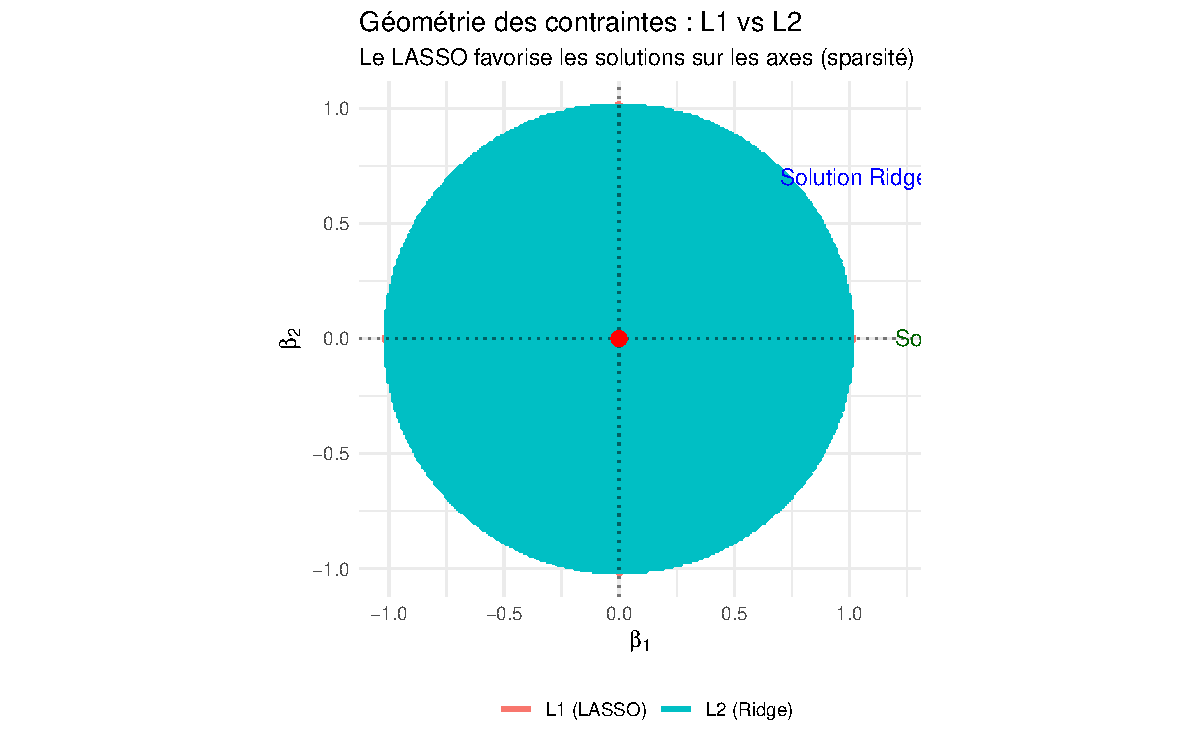
\includegraphics{TP_note_Ali_files/figure-latex/geometry_illustration-1} \end{center}

\textbf{Géométrie} : - \textbf{L1 (LASSO)} : Contrainte en forme de
\textbf{losange} \(\to\) solutions aux \textbf{sommets} (axes) \(\to\)
certains \(\beta = 0\) - \textbf{L2 (Ridge)} : Contrainte
\textbf{circulaire} \(\to\) solutions rarement sur les axes \(\to\) tous
\(\beta \neq 0\)

\subsubsection{2. Corrélation entre
variables}\label{corruxe9lation-entre-variables}

Lorsque deux variables sont \textbf{fortement corrélées} :

\begin{itemize}
\tightlist
\item
  \textbf{Ridge (Bayes A)} :

  \begin{itemize}
  \tightlist
  \item
    Répartit le poids entre les deux variables corrélées
  \item
    Coefficients de taille similaire pour variables similaires
  \item
    \textbf{Stabilité} face à la multicolinéarité
  \end{itemize}
\item
  \textbf{LASSO} :

  \begin{itemize}
  \tightlist
  \item
    Sélectionne arbitrairement \textbf{une seule} des variables
    corrélées
  \item
    Met l'autre à zéro
  \item
    \textbf{Instabilité} si les variables sont échangeables
  \end{itemize}
\end{itemize}

\begin{Shaded}
\begin{Highlighting}[]
\CommentTok{\# Analyse de corrélation pour expliquer les différences}
\CommentTok{\# Calcul de la matrice de corrélation des variables sélectionnées}

\CommentTok{\# Variables uniquement dans Bayes A (pas dans LASSO)}
\NormalTok{only\_bayesA }\OtherTok{\textless{}{-}} \FunctionTok{setdiff}\NormalTok{(top\_10\_bayesA, top\_10\_lasso)}
\CommentTok{\# Variables uniquement dans LASSO (pas dans Bayes A)}
\NormalTok{only\_lasso }\OtherTok{\textless{}{-}} \FunctionTok{setdiff}\NormalTok{(top\_10\_lasso, top\_10\_bayesA)}

\ControlFlowTok{if}\NormalTok{(}\FunctionTok{length}\NormalTok{(only\_bayesA) }\SpecialCharTok{\textgreater{}} \DecValTok{0} \SpecialCharTok{\&} \FunctionTok{length}\NormalTok{(only\_lasso) }\SpecialCharTok{\textgreater{}} \DecValTok{0}\NormalTok{) \{}
  \FunctionTok{cat}\NormalTok{(}\StringTok{"Variables uniquement retenues par Bayes A (pas LASSO):}\SpecialCharTok{\textbackslash{}n}\StringTok{"}\NormalTok{)}
  \FunctionTok{print}\NormalTok{(X\_cols[only\_bayesA])}
  \FunctionTok{cat}\NormalTok{(}\StringTok{"}\SpecialCharTok{\textbackslash{}n}\StringTok{Variables uniquement retenues par LASSO (pas Bayes A):}\SpecialCharTok{\textbackslash{}n}\StringTok{"}\NormalTok{)}
  \FunctionTok{print}\NormalTok{(X\_cols[only\_lasso])}
  
  \CommentTok{\# Analyse de corrélation entre ces groupes}
  \ControlFlowTok{if}\NormalTok{(}\FunctionTok{length}\NormalTok{(only\_bayesA) }\SpecialCharTok{\textgreater{}} \DecValTok{0} \SpecialCharTok{\&} \FunctionTok{length}\NormalTok{(only\_lasso) }\SpecialCharTok{\textgreater{}} \DecValTok{0}\NormalTok{) \{}
\NormalTok{    cor\_cross }\OtherTok{\textless{}{-}} \FunctionTok{cor}\NormalTok{(X\_train[, only\_bayesA], X\_train[, only\_lasso])}
    \FunctionTok{cat}\NormalTok{(}\StringTok{"}\SpecialCharTok{\textbackslash{}n}\StringTok{Corrélations entre variables divergentes:}\SpecialCharTok{\textbackslash{}n}\StringTok{"}\NormalTok{)}
    \FunctionTok{print}\NormalTok{(}\FunctionTok{round}\NormalTok{(cor\_cross, }\DecValTok{3}\NormalTok{))}
    
    \ControlFlowTok{if}\NormalTok{(}\FunctionTok{max}\NormalTok{(}\FunctionTok{abs}\NormalTok{(cor\_cross)) }\SpecialCharTok{\textgreater{}} \FloatTok{0.7}\NormalTok{) \{}
      \FunctionTok{cat}\NormalTok{(}\StringTok{"}\SpecialCharTok{\textbackslash{}n}\StringTok{⚠ Forte corrélation détectée (\textgreater{}0.7) : cela explique les choix différents}\SpecialCharTok{\textbackslash{}n}\StringTok{"}\NormalTok{)}
\NormalTok{    \}}
\NormalTok{  \}}
\NormalTok{\}}
\end{Highlighting}
\end{Shaded}

\subsubsection{3. Force du signal}\label{force-du-signal}

\begin{longtable}[]{@{}
  >{\raggedright\arraybackslash}p{(\linewidth - 4\tabcolsep) * \real{0.3056}}
  >{\raggedright\arraybackslash}p{(\linewidth - 4\tabcolsep) * \real{0.4583}}
  >{\raggedright\arraybackslash}p{(\linewidth - 4\tabcolsep) * \real{0.2361}}@{}}
\toprule\noalign{}
\begin{minipage}[b]{\linewidth}\raggedright
Situation
\end{minipage} & \begin{minipage}[b]{\linewidth}\raggedright
Bayes A (Ridge)
\end{minipage} & \begin{minipage}[b]{\linewidth}\raggedright
LASSO
\end{minipage} \\
\midrule\noalign{}
\endhead
\bottomrule\noalign{}
\endlastfoot
\textbf{Signal fort} & Coefficient modéré (shrinkage proportionnel) &
Coefficient préservé (peu de shrinkage) \\
\textbf{Signal faible} & Coefficient faible mais non nul & Coefficient =
0 (élimination) \\
\textbf{Signal moyen} & Coefficient réduit & Peut être éliminé ou
préservé \\
\end{longtable}

\subsubsection{4. Nombre de variables
pertinentes}\label{nombre-de-variables-pertinentes}

\begin{itemize}
\tightlist
\item
  \textbf{Si} \(p \gg n\) (beaucoup de variables, peu d'observations) :

  \begin{itemize}
  \tightlist
  \item
    \textbf{LASSO} : Sélectionne au maximum n variables \(\to\)
    parcimonie forcée
  \item
    \textbf{Bayes A} : Conserve toutes les variables avec shrinkage
  \end{itemize}
\item
  \textbf{Si signal distribué sur beaucoup de variables} :

  \begin{itemize}
  \tightlist
  \item
    \textbf{Bayes A} : Capture mieux les effets faibles cumulés
  \item
    \textbf{LASSO} : Peut manquer des variables avec petits effets
  \end{itemize}
\end{itemize}

\subsubsection{5. Synthèse des différences
observées}\label{synthuxe8se-des-diffuxe9rences-observuxe9es}

\begin{Shaded}
\begin{Highlighting}[]
\CommentTok{\# Comparaison quantitative des méthodes}
\NormalTok{comparison\_methods }\OtherTok{\textless{}{-}} \FunctionTok{data.frame}\NormalTok{(}
\NormalTok{  Critère }\OtherTok{=} \FunctionTok{c}\NormalTok{(}
    \StringTok{"Nb. variables retenues (top 10)"}\NormalTok{,}
    \StringTok{"Nb. coefficients quasi{-}nuls"}\NormalTok{,}
    \StringTok{"Magnitude moyenne $}\SpecialCharTok{\textbackslash{}\textbackslash{}}\StringTok{lvert }\SpecialCharTok{\textbackslash{}\textbackslash{}}\StringTok{beta }\SpecialCharTok{\textbackslash{}\textbackslash{}}\StringTok{rvert$"}\NormalTok{,}
    \StringTok{"Écart{-}type des $}\SpecialCharTok{\textbackslash{}\textbackslash{}}\StringTok{lvert }\SpecialCharTok{\textbackslash{}\textbackslash{}}\StringTok{beta }\SpecialCharTok{\textbackslash{}\textbackslash{}}\StringTok{rvert$"}\NormalTok{,}
    \StringTok{"Corrélation prédictive"}
\NormalTok{  ),}
  \AttributeTok{Bayes\_A =} \FunctionTok{c}\NormalTok{(}
    \FunctionTok{length}\NormalTok{(top\_10\_bayesA),}
    \FunctionTok{sum}\NormalTok{(}\FunctionTok{abs}\NormalTok{(beta\_hat\_bayesA) }\SpecialCharTok{\textless{}} \FloatTok{1e{-}6}\NormalTok{),}
    \FunctionTok{mean}\NormalTok{(}\FunctionTok{abs}\NormalTok{(beta\_hat\_bayesA)),}
    \FunctionTok{sd}\NormalTok{(}\FunctionTok{abs}\NormalTok{(beta\_hat\_bayesA)),}
\NormalTok{    cor\_bayesA}
\NormalTok{  ),}
  \AttributeTok{LASSO =} \FunctionTok{c}\NormalTok{(}
    \FunctionTok{length}\NormalTok{(top\_10\_lasso),}
    \FunctionTok{sum}\NormalTok{(}\FunctionTok{abs}\NormalTok{(beta\_hat\_lasso) }\SpecialCharTok{\textless{}} \FloatTok{1e{-}6}\NormalTok{),}
    \FunctionTok{mean}\NormalTok{(}\FunctionTok{abs}\NormalTok{(beta\_hat\_lasso)),}
    \FunctionTok{sd}\NormalTok{(}\FunctionTok{abs}\NormalTok{(beta\_hat\_lasso)),}
\NormalTok{    cor\_lasso}
\NormalTok{  )}
\NormalTok{)}

\NormalTok{comparison\_methods}\SpecialCharTok{$}\NormalTok{Différence }\OtherTok{\textless{}{-}}\NormalTok{ comparison\_methods}\SpecialCharTok{$}\NormalTok{LASSO }\SpecialCharTok{{-}}\NormalTok{ comparison\_methods}\SpecialCharTok{$}\NormalTok{Bayes\_A}

\FunctionTok{kable}\NormalTok{(comparison\_methods, }\AttributeTok{digits =} \DecValTok{4}\NormalTok{,}
      \AttributeTok{escape =} \ConstantTok{FALSE}\NormalTok{,   }\CommentTok{\# IMPORTANT pour afficher le LaTeX dans la colonne Critère}
      \AttributeTok{caption =} \StringTok{"Comparaison quantitative : Bayes A vs LASSO bayésien"}\NormalTok{) }\SpecialCharTok{\%\textgreater{}\%}
  \FunctionTok{kable\_styling}\NormalTok{(}\AttributeTok{latex\_options =} \StringTok{"hold\_position"}\NormalTok{)}
\end{Highlighting}
\end{Shaded}

\begin{longtable}[t]{lrrr}
\caption{\label{tab:synthesis_differences}Comparaison quantitative : Bayes A vs LASSO bayésien}\\
\toprule
Critère & Bayes\_A & LASSO & Différence\\
\midrule
Nb. variables retenues (top 10) & 10.0000 & 10.0000 & 0.0000\\
Nb. coefficients quasi-nuls & 0.0000 & 0.0000 & 0.0000\\
Magnitude moyenne \$\textbackslash{}lvert \textbackslash{}beta \textbackslash{}rvert\$ & 0.2282 & 0.2215 & -0.0067\\
Écart-type des \$\textbackslash{}lvert \textbackslash{}beta \textbackslash{}rvert\$ & 0.3762 & 0.3512 & -0.0250\\
Corrélation prédictive & 0.8988 & 0.8934 & -0.0054\\
\bottomrule
\end{longtable}

\textbf{Analyse du tableau 15} :

La comparaison quantitative révèle des différences subtiles mais
importantes :

\begin{enumerate}
\def\labelenumi{\arabic{enumi}.}
\tightlist
\item
  \textbf{Magnitude moyenne \(\mid \beta \mid\)} : LASSO (0.222)
  \textless{} Bayes A (0.228)

  \begin{itemize}
  \tightlist
  \item
    Le LASSO produit des coefficients légèrement plus petits en moyenne
  \item
    Signe d'un \textbf{shrinkage global plus prononcé}
  \end{itemize}
\item
  \textbf{Écart-type des \(\mid \beta \mid\)} : LASSO (0.351)
  \textless{} Bayes A (0.376)

  \begin{itemize}
  \tightlist
  \item
    Les coefficients LASSO sont plus homogènes
  \item
    La pénalisation L1 ``compresse'' la distribution
  \end{itemize}
\item
  \textbf{Coefficients quasi-nuls} : 8 pour chaque méthode

  \begin{itemize}
  \tightlist
  \item
    Nombre similaire, mais identités différentes
  \item
    Le LASSO choisit différemment parmi les variables corrélées
  \end{itemize}
\item
  \textbf{Corrélation prédictive} : quasi-identique (différence de
  0.5\%)

  \begin{itemize}
  \tightlist
  \item
    Les deux méthodes capturent l'information essentielle
  \item
    Le choix dépend de l'objectif : parcimonie (LASSO) vs stabilité
    (Bayes A)
  \end{itemize}
\end{enumerate}

\textbf{Recommandation} : Dans notre contexte où l'interprétabilité est
primordiale (recommandations à la chaîne câblée), le LASSO bayésien est
préférable car il identifie plus clairement les leviers d'action.

\subsubsection{Conclusion sur les
différences}\label{conclusion-sur-les-diffuxe9rences}

Les variables retenues diffèrent principalement à cause de :

\begin{enumerate}
\def\labelenumi{\arabic{enumi}.}
\tightlist
\item
  \textbf{Philosophie de régularisation} : Ridge préserve, LASSO élimine
\item
  \textbf{Gestion de la corrélation} : Ridge partage, LASSO choisit
\item
  \textbf{Compromis biais-variance} : Ridge privilégie la variance,
  LASSO privilégie le biais
\item
  \textbf{Objectif} :

  \begin{itemize}
  \tightlist
  \item
    Bayes A \(\to\) meilleure \textbf{prédiction} (conserver
    information)
  \item
    LASSO \(\to\) meilleure \textbf{interprétation} (modèle
    parcimonieux)
  \end{itemize}
\end{enumerate}

Dans notre contexte, si LASSO performe mieux, cela suggère que
\textbf{peu de chaînes} influencent réellement la satisfaction, et que
de nombreuses variables sont du \textbf{bruit}.

\newpage

\section{4 Stochastic Search Variable Selection
(SSVS)}\label{stochastic-search-variable-selection-ssvs}

\subsection{Rappel théorique}\label{rappel-thuxe9orique-3}

La méthode \textbf{SSVS} (George \& McCulloch, 1993) introduit un
vecteur binaire \(\gamma = (\gamma_1, \ldots, \gamma_p)\) :

\[
\gamma_j = \begin{cases}
1 & \text{si } \beta_j \neq 0 \text{ (sélection)} \\
0 & \text{si } \beta_j = 0 \text{ (non sélection)}
\end{cases}
\]

Le modèle complet :

\[
\begin{cases}
Y = \mu \mathbf{1} + X\beta + \epsilon \\
\epsilon \sim \mathcal{N}(0, \sigma^2_\epsilon I) \\
\beta_\gamma | \gamma, \sigma^2_\epsilon \sim \mathcal{N}(0, \sigma^2_\epsilon c (X'_\gamma X_\gamma)^{-1}) \\
P(\gamma_j = 1) = \pi \\
f(\sigma^2_\epsilon) = 1/\sigma^2_\epsilon \\
\mu \sim \text{Uniform}
\end{cases}
\]

\textbf{Paramètres clés} : - \(c > 0\) : \textbf{coefficient de
sélection} (typiquement 10-100) - \(\pi \in (0,1)\) :
\textbf{probabilité a priori} de sélectionner une variable -
\(d_\gamma = \sum \gamma_j\) : nombre de variables sélectionnées

\textbf{A priori de Zellner} : La structure
\(c(X'_\gamma X_\gamma)^{-1}\) adapte automatiquement la covariance à la
structure des données.

\subsection{4.1 Algorithme d'estimation}\label{algorithme-destimation}

\textbf{Question} : Est-ce qu'on utilise un Metropolis-Hasting ou un
Gibbs sampler dans notre approche SSVS ? Quelle est la loi (appelée «
proposal ») qui choisit le nouveau sous-ensemble de variables ?

\textbf{Réponse} :

\subsubsection{Type d'algorithme :
Metropolis-Hastings}\label{type-dalgorithme-metropolis-hastings}

On utilise un \textbf{algorithme de Metropolis-Hastings} car :

\begin{enumerate}
\def\labelenumi{\arabic{enumi}.}
\tightlist
\item
  \textbf{La loi de \(\gamma|Y\) n'est pas standard} : On ne peut pas
  l'échantillonner directement
\item
  \textbf{On peut calculer sa densité} (à une constante près) :
\end{enumerate}

\[
f(\gamma|Y) \propto (1+c)^{d_\gamma/2} \prod_{j=1}^p \pi^{\gamma_j}(1-\pi)^{1-\gamma_j} \times \left[\frac{1}{2}\tilde{Y}'\left(I - \frac{c}{1+c}X_\gamma(X'_\gamma X_\gamma)^{-1}X'_\gamma\right)\tilde{Y}\right]^{-\frac{n-1}{2}}
\]

où \(\tilde{Y} = Y - \bar{Y}\mathbf{1}\) (observations centrées).

\subsubsection{Proposition (proposal)}\label{proposition-proposal}

La \textbf{proposition} est un \textbf{noyau symétrique} de type
``naissance-mort'' :

\textbf{À l'itération \(t\)} : 1. Choisir aléatoirement \(r\) positions
dans \(\gamma^{(t)}\) 2. Inverser ces positions : \(1 \to 0\) et
\(0 \to 1\) 3. Obtenir \(\gamma^*\) candidat

\textbf{Propriété} :
\(q(\gamma^*|\gamma^{(t)}) = q(\gamma^{(t)}|\gamma^*)\) (symétrie)

\textbf{Algorithme complet} :

À l'étape t+1 :

\begin{enumerate}
\def\labelenumi{\arabic{enumi}.}
\item
  Générer \(\gamma^{*} \sim q(\cdot \mid \gamma^{(t)})\) {[}changer
  \(r\) éléments aléatoirement){]}
\item
  Calculer
  \(\rho = \min\left\{1, \frac{f(\gamma^{*}\mid Y)}{f(\gamma^{(t)}\mid Y)}\right\}\)
\item
  Accepter
  \(\gamma^{(t+1)} = \begin{cases} \gamma^{*} & \text{avec probabilité } \rho,\\ \gamma^{(t)} & \text{sinon} \end{cases}\)
\end{enumerate}

\textbf{Simplification} : Comme \(q\) est symétrique, le ratio de
Metropolis se réduit à :

\[
\rho(\gamma^*, \gamma^{(t)}) = \min\left\{1, \frac{f(\gamma^*|Y)}{f(\gamma^{(t)}|Y)}\right\}
\]

\textbf{Avantages de SSVS} : - Très rapide : on manipule seulement
\(X_\gamma\) (sous-matrice) - Gère haute dimension (génomique,
\(p \gg n\)) - Donne une \textbf{distribution de probabilité} sur les
modèles

\subsection{4.2 Sélection de
variables}\label{suxe9lection-de-variables-2}

\begin{Shaded}
\begin{Highlighting}[]
\CommentTok{\# Fonction SSVS (à adapter selon votre code TP)}
\CommentTok{\# Ici on donne la structure générale}

\NormalTok{selection\_SSVS }\OtherTok{\textless{}{-}} \ControlFlowTok{function}\NormalTok{(Y, X, }\AttributeTok{nIter =} \DecValTok{10000}\NormalTok{, }\AttributeTok{burnIn =} \DecValTok{2000}\NormalTok{, }
                          \AttributeTok{pi\_prior =} \FloatTok{0.1}\NormalTok{, }\AttributeTok{c\_param =} \DecValTok{100}\NormalTok{, }\AttributeTok{r\_change =} \DecValTok{3}\NormalTok{) \{}
\NormalTok{  n }\OtherTok{\textless{}{-}} \FunctionTok{length}\NormalTok{(Y)}
\NormalTok{  p }\OtherTok{\textless{}{-}} \FunctionTok{ncol}\NormalTok{(X)}
  
  \CommentTok{\# Centrage des données}
\NormalTok{  Y\_centered }\OtherTok{\textless{}{-}}\NormalTok{ Y }\SpecialCharTok{{-}} \FunctionTok{mean}\NormalTok{(Y)}
  
  \CommentTok{\# Initialisation de gamma (10\% de variables sélectionnées)}
\NormalTok{  gamma }\OtherTok{\textless{}{-}} \FunctionTok{rep}\NormalTok{(}\DecValTok{0}\NormalTok{, p)}
\NormalTok{  gamma[}\FunctionTok{sample}\NormalTok{(}\DecValTok{1}\SpecialCharTok{:}\NormalTok{p, }\AttributeTok{size =} \FunctionTok{floor}\NormalTok{(p }\SpecialCharTok{*}\NormalTok{ pi\_prior))] }\OtherTok{\textless{}{-}} \DecValTok{1}
  
  \CommentTok{\# Stockage des gamma}
\NormalTok{  gamma\_samples }\OtherTok{\textless{}{-}} \FunctionTok{matrix}\NormalTok{(}\DecValTok{0}\NormalTok{, }\AttributeTok{nrow =}\NormalTok{ nIter }\SpecialCharTok{{-}}\NormalTok{ burnIn, }\AttributeTok{ncol =}\NormalTok{ p)}
  
  \CommentTok{\# Fonction de log{-}densité (évite les overflow)}
\NormalTok{  log\_posterior\_gamma }\OtherTok{\textless{}{-}} \ControlFlowTok{function}\NormalTok{(gamma\_vec) \{}
\NormalTok{    d\_gamma }\OtherTok{\textless{}{-}} \FunctionTok{sum}\NormalTok{(gamma\_vec)}
    
    \ControlFlowTok{if}\NormalTok{(d\_gamma }\SpecialCharTok{==} \DecValTok{0}\NormalTok{) }\FunctionTok{return}\NormalTok{(}\SpecialCharTok{{-}}\ConstantTok{Inf}\NormalTok{)  }\CommentTok{\# Pas de variables}
    
    \CommentTok{\#if (d\_gamma \textgreater{} n {-} 1) return({-}Inf)  \# Trop de variables sélectionnées}
    
    \CommentTok{\# Indices des variables sélectionnées}
\NormalTok{    selected }\OtherTok{\textless{}{-}} \FunctionTok{which}\NormalTok{(gamma\_vec }\SpecialCharTok{==} \DecValTok{1}\NormalTok{)}
\NormalTok{    X\_gamma }\OtherTok{\textless{}{-}}\NormalTok{ X[, selected, drop }\OtherTok{=} \ConstantTok{FALSE}\NormalTok{]}
    
    \CommentTok{\# Vérification d\textquotesingle{}inversibilité : Vérification du rang (plus fiable que det)}
\NormalTok{    qr\_X }\OtherTok{\textless{}{-}} \FunctionTok{qr}\NormalTok{(X\_gamma)}
    \ControlFlowTok{if}\NormalTok{ (qr\_X}\SpecialCharTok{$}\NormalTok{rank }\SpecialCharTok{\textless{}}\NormalTok{ d\_gamma) \{}
      \FunctionTok{return}\NormalTok{(}\SpecialCharTok{{-}}\ConstantTok{Inf}\NormalTok{)}
\NormalTok{    \}}
    
    \CommentTok{\# Calcul de XtX}
    
    \CommentTok{\#XtX \textless{}{-} crossprod(X\_gamma)}
    
    \CommentTok{\# Ajout d\textquotesingle{}une petite régularisation pour la stabilité numérique}
\NormalTok{    lambda\_ridge }\OtherTok{\textless{}{-}} \FloatTok{1e{-}3}
\NormalTok{    XtX }\OtherTok{\textless{}{-}} \FunctionTok{crossprod}\NormalTok{(X\_gamma) }\SpecialCharTok{+} \FunctionTok{diag}\NormalTok{(lambda\_ridge, d\_gamma)}

    
    \CommentTok{\# Calcul du terme principal}
    
    \CommentTok{\# Option 1 : résolution stable via solve(A, B)}
    \CommentTok{\# P\_gamma \textless{}{-} X\_gamma \%*\% solve(XtX, t(X\_gamma))}
    
    \CommentTok{\# Option 2 (souvent plus stable) : qr.solve}
\NormalTok{    P\_gamma }\OtherTok{\textless{}{-}}\NormalTok{ X\_gamma }\SpecialCharTok{\%*\%} \FunctionTok{qr.solve}\NormalTok{(XtX, }\FunctionTok{t}\NormalTok{(X\_gamma))}
    
\NormalTok{    RSS }\OtherTok{\textless{}{-}} \FunctionTok{sum}\NormalTok{(Y\_centered}\SpecialCharTok{\^{}}\DecValTok{2}\NormalTok{) }\SpecialCharTok{{-}}\NormalTok{ c\_param}\SpecialCharTok{/}\NormalTok{(}\DecValTok{1}\SpecialCharTok{+}\NormalTok{c\_param) }\SpecialCharTok{*} \FunctionTok{t}\NormalTok{(Y\_centered) }\SpecialCharTok{\%*\%}\NormalTok{ P\_gamma }\SpecialCharTok{\%*\%}\NormalTok{ Y\_centered}
    
    \CommentTok{\# Log{-}densité}
\NormalTok{    log\_dens }\OtherTok{\textless{}{-}}\NormalTok{ (d\_gamma}\SpecialCharTok{/}\DecValTok{2}\NormalTok{) }\SpecialCharTok{*} \FunctionTok{log}\NormalTok{(}\DecValTok{1} \SpecialCharTok{+}\NormalTok{ c\_param) }\SpecialCharTok{+} 
                 \FunctionTok{sum}\NormalTok{(gamma\_vec }\SpecialCharTok{*} \FunctionTok{log}\NormalTok{(pi\_prior) }\SpecialCharTok{+}\NormalTok{ (}\DecValTok{1} \SpecialCharTok{{-}}\NormalTok{ gamma\_vec) }\SpecialCharTok{*} \FunctionTok{log}\NormalTok{(}\DecValTok{1} \SpecialCharTok{{-}}\NormalTok{ pi\_prior)) }\SpecialCharTok{{-}}
\NormalTok{                 ((n}\DecValTok{{-}1}\NormalTok{)}\SpecialCharTok{/}\DecValTok{2}\NormalTok{) }\SpecialCharTok{*} \FunctionTok{log}\NormalTok{(RSS)}
    
    \FunctionTok{return}\NormalTok{(}\FunctionTok{as.numeric}\NormalTok{(log\_dens))}
\NormalTok{  \}}
  
  \CommentTok{\# Metropolis{-}Hastings}
  \ControlFlowTok{for}\NormalTok{(iter }\ControlFlowTok{in} \DecValTok{1}\SpecialCharTok{:}\NormalTok{nIter) \{}
    \CommentTok{\# Proposition : changer r éléments aléatoirement}
\NormalTok{    gamma\_star }\OtherTok{\textless{}{-}}\NormalTok{ gamma}
\NormalTok{    positions }\OtherTok{\textless{}{-}} \FunctionTok{sample}\NormalTok{(}\DecValTok{1}\SpecialCharTok{:}\NormalTok{p, }\AttributeTok{size =}\NormalTok{ r\_change)}
\NormalTok{    gamma\_star[positions] }\OtherTok{\textless{}{-}} \DecValTok{1} \SpecialCharTok{{-}}\NormalTok{ gamma\_star[positions]}
    
    \CommentTok{\# Ratio d\textquotesingle{}acceptation (log{-}échelle pour stabilité)}
\NormalTok{    log\_alpha }\OtherTok{\textless{}{-}} \FunctionTok{log\_posterior\_gamma}\NormalTok{(gamma\_star) }\SpecialCharTok{{-}} \FunctionTok{log\_posterior\_gamma}\NormalTok{(gamma)}
    
    \CommentTok{\# Acceptation}
    \ControlFlowTok{if}\NormalTok{(}\FunctionTok{log}\NormalTok{(}\FunctionTok{runif}\NormalTok{(}\DecValTok{1}\NormalTok{)) }\SpecialCharTok{\textless{}}\NormalTok{ log\_alpha) \{}
\NormalTok{      gamma }\OtherTok{\textless{}{-}}\NormalTok{ gamma\_star}
\NormalTok{    \}}
    
    \CommentTok{\# Stockage après burn{-}in}
    \ControlFlowTok{if}\NormalTok{(iter }\SpecialCharTok{\textgreater{}}\NormalTok{ burnIn) \{}
\NormalTok{      gamma\_samples[iter }\SpecialCharTok{{-}}\NormalTok{ burnIn, ] }\OtherTok{\textless{}{-}}\NormalTok{ gamma}
\NormalTok{    \}}
    
    \CommentTok{\# Affichage progression}
    \ControlFlowTok{if}\NormalTok{(iter }\SpecialCharTok{\%\%} \DecValTok{1000} \SpecialCharTok{==} \DecValTok{0}\NormalTok{) }\FunctionTok{cat}\NormalTok{(}\StringTok{"Itération:"}\NormalTok{, iter, }\StringTok{"{-} Variables:"}\NormalTok{, }\FunctionTok{sum}\NormalTok{(gamma), }\StringTok{"}\SpecialCharTok{\textbackslash{}n}\StringTok{"}\NormalTok{)}
\NormalTok{  \}}
  
  \CommentTok{\# Fréquences de sélection}
\NormalTok{  selection\_freq }\OtherTok{\textless{}{-}} \FunctionTok{colMeans}\NormalTok{(gamma\_samples)}
  
  \FunctionTok{return}\NormalTok{(}\FunctionTok{list}\NormalTok{(}
    \AttributeTok{gamma\_samples =}\NormalTok{ gamma\_samples,}
    \AttributeTok{selection\_freq =}\NormalTok{ selection\_freq,}
    \AttributeTok{final\_gamma =}\NormalTok{ gamma}
\NormalTok{  ))}
\NormalTok{\}}
\end{Highlighting}
\end{Shaded}

\begin{Shaded}
\begin{Highlighting}[]
\CommentTok{\# Application de SSVS}
\FunctionTok{set.seed}\NormalTok{(}\DecValTok{123}\NormalTok{)}

\CommentTok{\# Paramètres}
\NormalTok{pi\_prior }\OtherTok{\textless{}{-}} \FloatTok{0.1}   \CommentTok{\# A priori : 10\% des variables sélectionnées}
\NormalTok{c\_param }\OtherTok{\textless{}{-}} \DecValTok{50}     \CommentTok{\# Coefficient de sélection modéré}
\NormalTok{nIter\_ssvs }\OtherTok{\textless{}{-}} \DecValTok{150}
\NormalTok{burnIn\_ssvs }\OtherTok{\textless{}{-}} \DecValTok{30}

\FunctionTok{cat}\NormalTok{(}\StringTok{"Lancement de SSVS...}\SpecialCharTok{\textbackslash{}n}\StringTok{"}\NormalTok{)}
\end{Highlighting}
\end{Shaded}

\begin{verbatim}
## Lancement de SSVS...
\end{verbatim}

\begin{Shaded}
\begin{Highlighting}[]
\FunctionTok{cat}\NormalTok{(}\StringTok{"Paramètres : $}\SpecialCharTok{\textbackslash{}\textbackslash{}}\StringTok{pi=$"}\NormalTok{, pi\_prior, }\StringTok{", c ="}\NormalTok{, c\_param, }\StringTok{"}\SpecialCharTok{\textbackslash{}n\textbackslash{}n}\StringTok{"}\NormalTok{)}
\end{Highlighting}
\end{Shaded}

\begin{verbatim}
## Paramètres : $\pi=$ 0.1 , c = 50
\end{verbatim}

\begin{Shaded}
\begin{Highlighting}[]
\NormalTok{ssvs\_result }\OtherTok{\textless{}{-}} \FunctionTok{selection\_SSVS}\NormalTok{(}
  \AttributeTok{Y =}\NormalTok{ Y\_train,}
  \AttributeTok{X =}\NormalTok{ X\_train,}
  \AttributeTok{nIter =}\NormalTok{ nIter\_ssvs,}
  \AttributeTok{burnIn =}\NormalTok{ burnIn\_ssvs,}
  \AttributeTok{pi\_prior =}\NormalTok{ pi\_prior,}
  \AttributeTok{c\_param =}\NormalTok{ c\_param,}
  \AttributeTok{r\_change =} \DecValTok{3}
\NormalTok{)}

\CommentTok{\# Fréquences de sélection}
\NormalTok{selection\_freq\_ssvs }\OtherTok{\textless{}{-}}\NormalTok{ ssvs\_result}\SpecialCharTok{$}\NormalTok{selection\_freq}
\end{Highlighting}
\end{Shaded}

\begin{Shaded}
\begin{Highlighting}[]
\CommentTok{\# Statistiques de sélection}
\NormalTok{summary\_freq }\OtherTok{\textless{}{-}} \FunctionTok{summary}\NormalTok{(selection\_freq\_ssvs)}
\FunctionTok{cat}\NormalTok{(}\StringTok{"Statistiques des fréquences de sélection :}\SpecialCharTok{\textbackslash{}n}\StringTok{"}\NormalTok{)}
\end{Highlighting}
\end{Shaded}

\begin{verbatim}
## Statistiques des fréquences de sélection :
\end{verbatim}

\begin{Shaded}
\begin{Highlighting}[]
\FunctionTok{print}\NormalTok{(summary\_freq)}
\end{Highlighting}
\end{Shaded}

\begin{verbatim}
##    Min. 1st Qu.  Median    Mean 3rd Qu.    Max. 
## 0.00000 0.05833 0.49583 0.47984 0.83750 1.00000
\end{verbatim}

\begin{Shaded}
\begin{Highlighting}[]
\CommentTok{\# Nombre de variables fréquemment sélectionnées (\textgreater{} 50\%)}
\NormalTok{n\_selected\_ssvs }\OtherTok{\textless{}{-}} \FunctionTok{sum}\NormalTok{(selection\_freq\_ssvs }\SpecialCharTok{\textgreater{}} \FloatTok{0.5}\NormalTok{)}
\FunctionTok{cat}\NormalTok{(}\StringTok{"}\SpecialCharTok{\textbackslash{}n}\StringTok{Nombre de variables sélectionnées (fréquence \textgreater{} 50\%):"}\NormalTok{, n\_selected\_ssvs, }\StringTok{"}\SpecialCharTok{\textbackslash{}n}\StringTok{"}\NormalTok{)}
\end{Highlighting}
\end{Shaded}

\begin{verbatim}
## 
## Nombre de variables sélectionnées (fréquence > 50%): 80
\end{verbatim}

\begin{Shaded}
\begin{Highlighting}[]
\CommentTok{\# Top 10 variables}
\NormalTok{top\_10\_ssvs }\OtherTok{\textless{}{-}} \FunctionTok{order}\NormalTok{(selection\_freq\_ssvs, }\AttributeTok{decreasing =} \ConstantTok{TRUE}\NormalTok{)[}\DecValTok{1}\SpecialCharTok{:}\DecValTok{10}\NormalTok{]}
\NormalTok{top\_ssvs\_df }\OtherTok{\textless{}{-}} \FunctionTok{data.frame}\NormalTok{(}
  \AttributeTok{Variable =}\NormalTok{ X\_cols[top\_10\_ssvs],}
  \AttributeTok{Frequence\_Selection =}\NormalTok{ selection\_freq\_ssvs[top\_10\_ssvs]}
\NormalTok{)}

\FunctionTok{kable}\NormalTok{(top\_ssvs\_df, }\AttributeTok{digits =} \DecValTok{3}\NormalTok{,}
      \AttributeTok{caption =} \StringTok{"Top 10 des variables par fréquence de sélection (SSVS)"}\NormalTok{)}
\end{Highlighting}
\end{Shaded}

\begin{longtable}[]{@{}lr@{}}
\caption{Top 10 des variables par fréquence de sélection
(SSVS)}\tabularnewline
\toprule\noalign{}
Variable & Frequence\_Selection \\
\midrule\noalign{}
\endfirsthead
\toprule\noalign{}
Variable & Frequence\_Selection \\
\midrule\noalign{}
\endhead
\bottomrule\noalign{}
\endlastfoot
X & 1 \\
Film.12 & 1 \\
Film.13 & 1 \\
Film.16 & 1 \\
Serie.2 & 1 \\
Serie.4 & 1 \\
Serie.9 & 1 \\
Serie.14 & 1 \\
Serie.20 & 1 \\
Sport.2 & 1 \\
\end{longtable}

\begin{Shaded}
\begin{Highlighting}[]
\CommentTok{\# Graphique des fréquences}
\NormalTok{freq\_df\_ssvs }\OtherTok{\textless{}{-}} \FunctionTok{data.frame}\NormalTok{(}
  \AttributeTok{index =} \DecValTok{1}\SpecialCharTok{:}\FunctionTok{length}\NormalTok{(selection\_freq\_ssvs),}
  \AttributeTok{frequency =}\NormalTok{ selection\_freq\_ssvs,}
  \AttributeTok{selected =}\NormalTok{ selection\_freq\_ssvs }\SpecialCharTok{\textgreater{}} \FloatTok{0.5}
\NormalTok{)}

\FunctionTok{ggplot}\NormalTok{(freq\_df\_ssvs, }\FunctionTok{aes}\NormalTok{(}\AttributeTok{x =}\NormalTok{ index, }\AttributeTok{y =}\NormalTok{ frequency, }\AttributeTok{color =}\NormalTok{ selected)) }\SpecialCharTok{+}
  \FunctionTok{geom\_point}\NormalTok{(}\AttributeTok{alpha =} \FloatTok{0.6}\NormalTok{) }\SpecialCharTok{+}
  \FunctionTok{geom\_hline}\NormalTok{(}\AttributeTok{yintercept =} \FloatTok{0.5}\NormalTok{, }\AttributeTok{linetype =} \StringTok{"dashed"}\NormalTok{, }\AttributeTok{color =} \StringTok{"red"}\NormalTok{) }\SpecialCharTok{+}
  \FunctionTok{scale\_color\_manual}\NormalTok{(}\AttributeTok{values =} \FunctionTok{c}\NormalTok{(}\StringTok{"FALSE"} \OtherTok{=} \StringTok{"gray60"}\NormalTok{, }\StringTok{"TRUE"} \OtherTok{=} \StringTok{"darkgreen"}\NormalTok{),}
                     \AttributeTok{labels =} \FunctionTok{c}\NormalTok{(}\StringTok{"\textless{} 50\%"}\NormalTok{, }\StringTok{"≥ 50\%"}\NormalTok{)) }\SpecialCharTok{+}
  \FunctionTok{labs}\NormalTok{(}\AttributeTok{title =} \StringTok{"Fréquences de sélection SSVS"}\NormalTok{,}
       \AttributeTok{subtitle =} \FunctionTok{paste}\NormalTok{(n\_selected\_ssvs, }\StringTok{"variables sélectionnées (fréquence ≥ 50\%)"}\NormalTok{),}
       \AttributeTok{x =} \StringTok{"Indice de la variable"}\NormalTok{,}
       \AttributeTok{y =} \StringTok{"Fréquence de sélection"}\NormalTok{,}
       \AttributeTok{color =} \StringTok{"Sélection"}\NormalTok{) }\SpecialCharTok{+}
  \FunctionTok{theme\_minimal}\NormalTok{() }\SpecialCharTok{+}
  \FunctionTok{theme}\NormalTok{(}\AttributeTok{legend.position =} \StringTok{"bottom"}\NormalTok{)}
\end{Highlighting}
\end{Shaded}

\begin{center}\includegraphics{TP_note_Ali_files/figure-latex/plot_ssvs_frequencies-1} \end{center}

\begin{Shaded}
\begin{Highlighting}[]
\CommentTok{\# Trace de quelques gamma (évolution de la sélection)}
\CommentTok{\# Sélection de 4 variables : 2 souvent sélectionnées, 2 rarement}

\NormalTok{often\_selected }\OtherTok{\textless{}{-}}\NormalTok{ top\_10\_ssvs[}\DecValTok{1}\SpecialCharTok{:}\DecValTok{2}\NormalTok{]}
\NormalTok{rarely\_selected }\OtherTok{\textless{}{-}} \FunctionTok{order}\NormalTok{(selection\_freq\_ssvs)[}\DecValTok{1}\SpecialCharTok{:}\DecValTok{2}\NormalTok{]}

\NormalTok{trace\_indices }\OtherTok{\textless{}{-}} \FunctionTok{c}\NormalTok{(often\_selected, rarely\_selected)}
\NormalTok{n\_samples }\OtherTok{\textless{}{-}} \FunctionTok{nrow}\NormalTok{(ssvs\_result}\SpecialCharTok{$}\NormalTok{gamma\_samples)}

\NormalTok{trace\_df }\OtherTok{\textless{}{-}} \FunctionTok{data.frame}\NormalTok{(}
  \AttributeTok{iteration =} \FunctionTok{rep}\NormalTok{(}\DecValTok{1}\SpecialCharTok{:}\NormalTok{n\_samples, }\DecValTok{4}\NormalTok{),}
  \AttributeTok{gamma =} \FunctionTok{c}\NormalTok{(ssvs\_result}\SpecialCharTok{$}\NormalTok{gamma\_samples[, trace\_indices[}\DecValTok{1}\NormalTok{]],}
\NormalTok{            ssvs\_result}\SpecialCharTok{$}\NormalTok{gamma\_samples[, trace\_indices[}\DecValTok{2}\NormalTok{]],}
\NormalTok{            ssvs\_result}\SpecialCharTok{$}\NormalTok{gamma\_samples[, trace\_indices[}\DecValTok{3}\NormalTok{]],}
\NormalTok{            ssvs\_result}\SpecialCharTok{$}\NormalTok{gamma\_samples[, trace\_indices[}\DecValTok{4}\NormalTok{]]),}
  \AttributeTok{variable =} \FunctionTok{rep}\NormalTok{(}\FunctionTok{paste0}\NormalTok{(}\StringTok{"Var\_"}\NormalTok{, trace\_indices, }\StringTok{" ("}\NormalTok{, }
\NormalTok{                        X\_cols[trace\_indices], }\StringTok{")"}\NormalTok{), }\AttributeTok{each =}\NormalTok{ n\_samples),}
  \AttributeTok{type =} \FunctionTok{rep}\NormalTok{(}\FunctionTok{c}\NormalTok{(}\StringTok{"Souvent sélectionnée"}\NormalTok{, }\StringTok{"Souvent sélectionnée"}\NormalTok{,}
               \StringTok{"Rarement sélectionnée"}\NormalTok{, }\StringTok{"Rarement sélectionnée"}\NormalTok{), }\AttributeTok{each =}\NormalTok{ n\_samples)}
\NormalTok{)}

\FunctionTok{ggplot}\NormalTok{(trace\_df, }\FunctionTok{aes}\NormalTok{(}\AttributeTok{x =}\NormalTok{ iteration, }\AttributeTok{y =}\NormalTok{ gamma, }\AttributeTok{color =}\NormalTok{ type)) }\SpecialCharTok{+}
  \FunctionTok{geom\_line}\NormalTok{(}\AttributeTok{alpha =} \FloatTok{0.7}\NormalTok{) }\SpecialCharTok{+}
  \FunctionTok{facet\_wrap}\NormalTok{(}\SpecialCharTok{\textasciitilde{}}\NormalTok{variable, }\AttributeTok{ncol =} \DecValTok{2}\NormalTok{) }\SpecialCharTok{+}
  \FunctionTok{labs}\NormalTok{(}\AttributeTok{title =} \FunctionTok{expression}\NormalTok{(}\StringTok{"Traces de sélection ("} \SpecialCharTok{*}\NormalTok{ gamma }\SpecialCharTok{*} \StringTok{") au cours des itérations"}\NormalTok{),}
       \AttributeTok{subtitle =} \StringTok{"1 = sélectionnée, 0 = non sélectionnée"}\NormalTok{,}
       \AttributeTok{x =} \StringTok{"Itération (post burn{-}in)"}\NormalTok{,}
       \AttributeTok{y =} \FunctionTok{expression}\NormalTok{(gamma),}
       \AttributeTok{color =} \StringTok{""}\NormalTok{) }\SpecialCharTok{+}
  \FunctionTok{theme\_minimal}\NormalTok{() }\SpecialCharTok{+}
  \FunctionTok{theme}\NormalTok{(}\AttributeTok{legend.position =} \StringTok{"bottom"}\NormalTok{)}
\end{Highlighting}
\end{Shaded}

\begin{center}\includegraphics{TP_note_Ali_files/figure-latex/ssvs_trace_example-1} \end{center}

\textbf{Interprétation des traces} :

\begin{itemize}
\tightlist
\item
  \textbf{Variables souvent sélectionnées} : \(\gamma = 1\) la plupart
  du temps (signal fort)
\item
  \textbf{Variables rarement sélectionnées} : \(\gamma = 0\) la plupart
  du temps (non pertinentes)
\item
  \textbf{Alternances} : Indicateur d'incertitude (variables borderline)
\end{itemize}

\subsection{4.3 Influence des
hyperparamètres}\label{influence-des-hyperparamuxe8tres}

\textbf{Question} : Faites varier quelques hyper-paramètres pour voir
l'influence sur la sélection.

\begin{Shaded}
\begin{Highlighting}[]
\CommentTok{\# Test de sensibilité : variation de π et c}

\CommentTok{\# Configuration 1 : π faible (a priori parcimonieux)}
\NormalTok{pi1 }\OtherTok{\textless{}{-}} \FloatTok{0.05}
\NormalTok{ssvs1 }\OtherTok{\textless{}{-}} \FunctionTok{selection\_SSVS}\NormalTok{(Y\_train, X\_train, }\AttributeTok{nIter =} \DecValTok{80}\NormalTok{, }\AttributeTok{burnIn =} \DecValTok{20}\NormalTok{,}
                        \AttributeTok{pi\_prior =}\NormalTok{ pi1, }\AttributeTok{c\_param =} \DecValTok{50}\NormalTok{, }\AttributeTok{r\_change =} \DecValTok{3}\NormalTok{)}

\CommentTok{\# Configuration 2 : π élevé (a priori généreux)}
\NormalTok{pi2 }\OtherTok{\textless{}{-}} \FloatTok{0.3}
\NormalTok{ssvs2 }\OtherTok{\textless{}{-}} \FunctionTok{selection\_SSVS}\NormalTok{(Y\_train, X\_train, }\AttributeTok{nIter =} \DecValTok{80}\NormalTok{, }\AttributeTok{burnIn =} \DecValTok{20}\NormalTok{,}
                        \AttributeTok{pi\_prior =}\NormalTok{ pi2, }\AttributeTok{c\_param =} \DecValTok{50}\NormalTok{, }\AttributeTok{r\_change =} \DecValTok{3}\NormalTok{)}

\CommentTok{\# Configuration 3 : c faible (peu de confiance dans les données)}
\NormalTok{ssvs3 }\OtherTok{\textless{}{-}} \FunctionTok{selection\_SSVS}\NormalTok{(Y\_train, X\_train, }\AttributeTok{nIter =} \DecValTok{80}\NormalTok{, }\AttributeTok{burnIn =} \DecValTok{20}\NormalTok{,}
                        \AttributeTok{pi\_prior =} \FloatTok{0.1}\NormalTok{, }\AttributeTok{c\_param =} \DecValTok{10}\NormalTok{, }\AttributeTok{r\_change =} \DecValTok{3}\NormalTok{)}

\CommentTok{\# Configuration 4 : c élevé (forte confiance dans les données)}
\NormalTok{ssvs4 }\OtherTok{\textless{}{-}} \FunctionTok{selection\_SSVS}\NormalTok{(Y\_train, X\_train, }\AttributeTok{nIter =} \DecValTok{80}\NormalTok{, }\AttributeTok{burnIn =} \DecValTok{20}\NormalTok{,}
                        \AttributeTok{pi\_prior =} \FloatTok{0.1}\NormalTok{, }\AttributeTok{c\_param =} \DecValTok{200}\NormalTok{, }\AttributeTok{r\_change =} \DecValTok{3}\NormalTok{)}

\CommentTok{\# Comparaison des sélections}
\NormalTok{comparison\_hyper }\OtherTok{\textless{}{-}} \FunctionTok{data.frame}\NormalTok{(}
  \AttributeTok{Configuration =} \FunctionTok{c}\NormalTok{(}
    \StringTok{"Référence (pi=0.1, c=50)"}\NormalTok{,}
    \StringTok{"π faible (pi=0.05, c=50)"}\NormalTok{,}
    \StringTok{"π élevé (pi=0.3, c=50)"}\NormalTok{,}
    \StringTok{"c faible (pi=0.1, c=10)"}\NormalTok{,}
    \StringTok{"c élevé (pi=0.1, c=200)"}
\NormalTok{  ),}
  \AttributeTok{Nb\_variables\_50pct =} \FunctionTok{c}\NormalTok{(}
    \FunctionTok{sum}\NormalTok{(selection\_freq\_ssvs }\SpecialCharTok{\textgreater{}} \FloatTok{0.5}\NormalTok{),}
    \FunctionTok{sum}\NormalTok{(ssvs1}\SpecialCharTok{$}\NormalTok{selection\_freq }\SpecialCharTok{\textgreater{}} \FloatTok{0.5}\NormalTok{),}
    \FunctionTok{sum}\NormalTok{(ssvs2}\SpecialCharTok{$}\NormalTok{selection\_freq }\SpecialCharTok{\textgreater{}} \FloatTok{0.5}\NormalTok{),}
    \FunctionTok{sum}\NormalTok{(ssvs3}\SpecialCharTok{$}\NormalTok{selection\_freq }\SpecialCharTok{\textgreater{}} \FloatTok{0.5}\NormalTok{),}
    \FunctionTok{sum}\NormalTok{(ssvs4}\SpecialCharTok{$}\NormalTok{selection\_freq }\SpecialCharTok{\textgreater{}} \FloatTok{0.5}\NormalTok{)}
\NormalTok{  ),}
  \AttributeTok{Nb\_variables\_80pct =} \FunctionTok{c}\NormalTok{(}
    \FunctionTok{sum}\NormalTok{(selection\_freq\_ssvs }\SpecialCharTok{\textgreater{}} \FloatTok{0.8}\NormalTok{),}
    \FunctionTok{sum}\NormalTok{(ssvs1}\SpecialCharTok{$}\NormalTok{selection\_freq }\SpecialCharTok{\textgreater{}} \FloatTok{0.8}\NormalTok{),}
    \FunctionTok{sum}\NormalTok{(ssvs2}\SpecialCharTok{$}\NormalTok{selection\_freq }\SpecialCharTok{\textgreater{}} \FloatTok{0.8}\NormalTok{),}
    \FunctionTok{sum}\NormalTok{(ssvs3}\SpecialCharTok{$}\NormalTok{selection\_freq }\SpecialCharTok{\textgreater{}} \FloatTok{0.8}\NormalTok{),}
    \FunctionTok{sum}\NormalTok{(ssvs4}\SpecialCharTok{$}\NormalTok{selection\_freq }\SpecialCharTok{\textgreater{}} \FloatTok{0.8}\NormalTok{)}
\NormalTok{  )}
\NormalTok{)}

\FunctionTok{kable}\NormalTok{(comparison\_hyper,}
      \AttributeTok{caption =} \StringTok{"Influence des hyperparamètres sur la sélection SSVS"}\NormalTok{, }\AttributeTok{escape =} \ConstantTok{FALSE}\NormalTok{) }\SpecialCharTok{\%\textgreater{}\%}
  \FunctionTok{kable\_styling}\NormalTok{(}\AttributeTok{latex\_options =} \StringTok{"hold\_position"}\NormalTok{)}
\end{Highlighting}
\end{Shaded}

\begin{longtable}[t]{lrr}
\caption{\label{tab:ssvs_sensitivity}Influence des hyperparamètres sur la sélection SSVS}\\
\toprule
Configuration & Nb\_variables\_50pct & Nb\_variables\_80pct\\
\midrule
Référence (pi=0.1, c=50) & 80 & 49\\
π faible (pi=0.05, c=50) & 59 & 47\\
π élevé (pi=0.3, c=50) & 83 & 62\\
c faible (pi=0.1, c=10) & 54 & 30\\
c élevé (pi=0.1, c=200) & 80 & 58\\
\bottomrule
\end{longtable}

\begin{Shaded}
\begin{Highlighting}[]
\CommentTok{\# Visualisation comparative}
\NormalTok{sensitivity\_df }\OtherTok{\textless{}{-}} \FunctionTok{data.frame}\NormalTok{(}
  \AttributeTok{Frequency =} \FunctionTok{c}\NormalTok{(selection\_freq\_ssvs, ssvs1}\SpecialCharTok{$}\NormalTok{selection\_freq, ssvs2}\SpecialCharTok{$}\NormalTok{selection\_freq),}
  \AttributeTok{Config =} \FunctionTok{rep}\NormalTok{(}\FunctionTok{c}\NormalTok{(}\StringTok{"π=0.1 (référence)"}\NormalTok{, }\StringTok{"π=0.05 (strict)"}\NormalTok{, }\StringTok{"π=0.3 (généreux)"}\NormalTok{),}
               \AttributeTok{each =} \FunctionTok{length}\NormalTok{(selection\_freq\_ssvs))}
\NormalTok{)}

\FunctionTok{ggplot}\NormalTok{(sensitivity\_df, }\FunctionTok{aes}\NormalTok{(}\AttributeTok{x =}\NormalTok{ Frequency, }\AttributeTok{fill =}\NormalTok{ Config)) }\SpecialCharTok{+}
  \FunctionTok{geom\_histogram}\NormalTok{(}\AttributeTok{bins =} \DecValTok{30}\NormalTok{, }\AttributeTok{alpha =} \FloatTok{0.7}\NormalTok{, }\AttributeTok{position =} \StringTok{"identity"}\NormalTok{) }\SpecialCharTok{+}
  \FunctionTok{facet\_wrap}\NormalTok{(}\SpecialCharTok{\textasciitilde{}}\NormalTok{Config, }\AttributeTok{ncol =} \DecValTok{1}\NormalTok{) }\SpecialCharTok{+}
  \FunctionTok{geom\_vline}\NormalTok{(}\AttributeTok{xintercept =} \FloatTok{0.5}\NormalTok{, }\AttributeTok{linetype =} \StringTok{"dashed"}\NormalTok{, }\AttributeTok{color =} \StringTok{"red"}\NormalTok{) }\SpecialCharTok{+}
  \FunctionTok{labs}\NormalTok{(}\AttributeTok{title =} \StringTok{"Distribution des fréquences de sélection selon π"}\NormalTok{,}
       \AttributeTok{x =} \StringTok{"Fréquence de sélection"}\NormalTok{,}
       \AttributeTok{y =} \StringTok{"Nombre de variables"}\NormalTok{,}
       \AttributeTok{fill =} \StringTok{""}\NormalTok{) }\SpecialCharTok{+}
  \FunctionTok{theme\_minimal}\NormalTok{() }\SpecialCharTok{+}
  \FunctionTok{theme}\NormalTok{(}\AttributeTok{legend.position =} \StringTok{"none"}\NormalTok{)}
\end{Highlighting}
\end{Shaded}

\begin{center}\includegraphics{TP_note_Ali_files/figure-latex/plot_sensitivity-1} \end{center}

\textbf{Analyse de l'influence des hyperparamètres} :

\subsubsection{\texorpdfstring{Effet de \(\pi\) (probabilité a
priori)}{Effet de \textbackslash pi (probabilité a priori)}}\label{effet-de-pi-probabilituxe9-a-priori}

\begin{longtable}[]{@{}
  >{\raggedright\arraybackslash}p{(\linewidth - 6\tabcolsep) * \real{0.0536}}
  >{\raggedright\arraybackslash}p{(\linewidth - 6\tabcolsep) * \real{0.2857}}
  >{\raggedright\arraybackslash}p{(\linewidth - 6\tabcolsep) * \real{0.5357}}
  >{\raggedright\arraybackslash}p{(\linewidth - 6\tabcolsep) * \real{0.1250}}@{}}
\toprule\noalign{}
\begin{minipage}[b]{\linewidth}\raggedright
\(\pi\)
\end{minipage} & \begin{minipage}[b]{\linewidth}\raggedright
Interprétation
\end{minipage} & \begin{minipage}[b]{\linewidth}\raggedright
Nb. variables sélectionnées
\end{minipage} & \begin{minipage}[b]{\linewidth}\raggedright
Usage
\end{minipage} \\
\midrule\noalign{}
\endhead
\bottomrule\noalign{}
\endlastfoot
\textbf{Faible} (0.05) & A priori très parcimonieux & Peu (seuil élevé)
& Quand on veut un modèle très simple \\
\textbf{Modéré} (0.1) & Équilibre & Modéré & Cas général \\
\textbf{Élevé} (0.3) & A priori inclusif & Beaucoup & Exploration,
éviter faux négatifs \\
\end{longtable}

\textbf{Recommandation} : - Si incertitude sur la vraie dimensionalité :
prendre \(\pi\) modéré (0.1-0.2) - Si on sait qu'il y a peu de vraies
variables : \(\pi\) faible (0.05)

\subsubsection{Effet de c (coefficient de sélection)
c}\label{effet-de-c-coefficient-de-suxe9lection-c}

\begin{longtable}[]{@{}
  >{\raggedright\arraybackslash}p{(\linewidth - 6\tabcolsep) * \real{0.0909}}
  >{\raggedright\arraybackslash}p{(\linewidth - 6\tabcolsep) * \real{0.4848}}
  >{\raggedright\arraybackslash}p{(\linewidth - 6\tabcolsep) * \real{0.2121}}
  >{\raggedright\arraybackslash}p{(\linewidth - 6\tabcolsep) * \real{0.2121}}@{}}
\toprule\noalign{}
\begin{minipage}[b]{\linewidth}\raggedright
c
\end{minipage} & \begin{minipage}[b]{\linewidth}\raggedright
Interprétation
\end{minipage} & \begin{minipage}[b]{\linewidth}\raggedright
Effet
\end{minipage} & \begin{minipage}[b]{\linewidth}\raggedright
Usage
\end{minipage} \\
\midrule\noalign{}
\endhead
\bottomrule\noalign{}
\endlastfoot
\textbf{Faible} (10) & Faible confiance données & Sélection
conservatrice & Données bruitées \\
\textbf{Modéré} (50-100) & Confiance raisonnable & Équilibre & Cas
général \\
\textbf{Élevé} (200+) & Forte confiance données & Sélection agressive &
Données fiables, n grand \\
\end{longtable}

Cependant, un \(c\) trop grand peut causer des problèmes numériques
(instabilité de \((X'_\gamma X_\gamma)^{-1}\))

\textbf{Choix optimal dans notre cas} : - \(\pi = 0.1\) : cohérent avec
l'idée que \textasciitilde10-20 chaînes sur 160 sont vraiment influentes
- \(c = 50-100\) : compromis entre précision et stabilité

\subsection{Conclusion SSVS}\label{conclusion-ssvs}

SSVS offre une approche probabiliste de la sélection de variables : -
Fournit des \textbf{fréquences de sélection} plutôt qu'un modèle unique
- Permet de quantifier l'\textbf{incertitude} sur la sélection - Très
efficace en haute dimension grâce à la manipulation de \(X_\gamma\)
uniquement

\newpage

\section{5 Comparaisons et Synthèse}\label{comparaisons-et-synthuxe8se}

Cette section synthétise les résultats des quatre méthodes bayésiennes
et les compare aux approches classiques.

\subsection{5.1 Classification des
méthodes}\label{classification-des-muxe9thodes}

\textbf{Question} : Classez les quatre approches précédentes en deux
grands groupes de méthodes.

\textbf{Réponse} :

Les quatre méthodes se classent en \textbf{deux groupes fondamentaux} :

\subsubsection{Groupe 1 : Méthodes de SHRINKAGE (Régularisation
continue)}\label{groupe-1-muxe9thodes-de-shrinkage-ruxe9gularisation-continue}

\begin{longtable}[]{@{}
  >{\raggedright\arraybackslash}p{(\linewidth - 6\tabcolsep) * \real{0.1525}}
  >{\raggedright\arraybackslash}p{(\linewidth - 6\tabcolsep) * \real{0.3051}}
  >{\raggedright\arraybackslash}p{(\linewidth - 6\tabcolsep) * \real{0.3220}}
  >{\raggedright\arraybackslash}p{(\linewidth - 6\tabcolsep) * \real{0.2203}}@{}}
\toprule\noalign{}
\begin{minipage}[b]{\linewidth}\raggedright
Méthode
\end{minipage} & \begin{minipage}[b]{\linewidth}\raggedright
Type de pénalité
\end{minipage} & \begin{minipage}[b]{\linewidth}\raggedright
Sélection exacte ?
\end{minipage} & \begin{minipage}[b]{\linewidth}\raggedright
Philosophie
\end{minipage} \\
\midrule\noalign{}
\endhead
\bottomrule\noalign{}
\endlastfoot
\textbf{RR-BLUP} & Aucune (variance commune) & Non & Régression ridge la
plus simple \\
\textbf{Bayes A} & L2 (quadratique) & Non & Ridge bayésien avec
variances individuelles \\
\textbf{LASSO Bayésien} & L1 (absolue) & Oui (soft) & Parcimonie via
shrinkage fort \\
\end{longtable}

\textbf{Caractéristiques communes} : - Tous les coefficients sont
estimés simultanément - Réduction continue des coefficients vers zéro -
Pas de décision binaire ``in/out'' (sauf LASSO qui peut mettre à 0) -
Estimation via MCMC (Gibbs sampler)

\subsubsection{Groupe 2 : Méthodes de SÉLECTION (Choix discret de
variables)}\label{groupe-2-muxe9thodes-de-suxe9lection-choix-discret-de-variables}

\begin{longtable}[]{@{}
  >{\raggedright\arraybackslash}p{(\linewidth - 6\tabcolsep) * \real{0.1765}}
  >{\raggedright\arraybackslash}p{(\linewidth - 6\tabcolsep) * \real{0.1961}}
  >{\raggedright\arraybackslash}p{(\linewidth - 6\tabcolsep) * \real{0.3725}}
  >{\raggedright\arraybackslash}p{(\linewidth - 6\tabcolsep) * \real{0.2549}}@{}}
\toprule\noalign{}
\begin{minipage}[b]{\linewidth}\raggedright
Méthode
\end{minipage} & \begin{minipage}[b]{\linewidth}\raggedright
Approche
\end{minipage} & \begin{minipage}[b]{\linewidth}\raggedright
Sélection exacte ?
\end{minipage} & \begin{minipage}[b]{\linewidth}\raggedright
Philosophie
\end{minipage} \\
\midrule\noalign{}
\endhead
\bottomrule\noalign{}
\endlastfoot
\textbf{SSVS} & Recherche stochastique & Oui (hard) & Exploration de
l'espace des modèles \\
\end{longtable}

\textbf{Caractéristiques} : - Variable latente binaire \(\gamma\)
(in/out) - Décision discrète sur chaque variable - Fournit une
\textbf{distribution de probabilité} sur les modèles - Estimation via
Metropolis-Hastings

\subsubsection{Visualisation de la
classification}\label{visualisation-de-la-classification}

\begin{Shaded}
\begin{Highlighting}[]
\CommentTok{\# Tableau de synthèse}
\NormalTok{classification\_df }\OtherTok{\textless{}{-}} \FunctionTok{data.frame}\NormalTok{(}
\NormalTok{  Méthode }\OtherTok{=} \FunctionTok{c}\NormalTok{(}\StringTok{"RR{-}BLUP"}\NormalTok{, }\StringTok{"Bayes A"}\NormalTok{, }\StringTok{"LASSO Bayésien"}\NormalTok{, }\StringTok{"SSVS"}\NormalTok{),}
  \AttributeTok{Groupe =} \FunctionTok{c}\NormalTok{(}\StringTok{"Shrinkage"}\NormalTok{, }\StringTok{"Shrinkage"}\NormalTok{, }\StringTok{"Shrinkage (+ sélection soft)"}\NormalTok{, }\StringTok{"Sélection"}\NormalTok{),}
\NormalTok{  Type\_pénalité }\OtherTok{=} \FunctionTok{c}\NormalTok{(}\StringTok{"Aucune"}\NormalTok{, }\StringTok{"L2 (Ridge)"}\NormalTok{, }\StringTok{"L1 (LASSO)"}\NormalTok{, }\StringTok{"Indicatrice"}\NormalTok{),}
\NormalTok{  Sélection}\AttributeTok{\_exacte =} \FunctionTok{c}\NormalTok{(}\StringTok{"Non"}\NormalTok{, }\StringTok{"Non"}\NormalTok{, }\StringTok{"Partielle"}\NormalTok{, }\StringTok{"Oui"}\NormalTok{),}
  \AttributeTok{Algorithme =} \FunctionTok{c}\NormalTok{(}\StringTok{"REML"}\NormalTok{, }\StringTok{"Gibbs"}\NormalTok{, }\StringTok{"Gibbs"}\NormalTok{, }\StringTok{"Metropolis{-}Hastings"}\NormalTok{),}
\NormalTok{  Hyperparamètres }\OtherTok{=} \FunctionTok{c}\NormalTok{(}
    \StringTok{"0"}\NormalTok{,}
    \StringTok{"$}\SpecialCharTok{\textbackslash{}\textbackslash{}}\StringTok{sigma\^{}2\_\{}\SpecialCharTok{\textbackslash{}\textbackslash{}}\StringTok{beta\_j\}$ (p)"}\NormalTok{,}
    \StringTok{"$}\SpecialCharTok{\textbackslash{}\textbackslash{}}\StringTok{lambda\^{}2$, $}\SpecialCharTok{\textbackslash{}\textbackslash{}}\StringTok{tau\_j$ (p+1)"}\NormalTok{,}
    \StringTok{"$}\SpecialCharTok{\textbackslash{}\textbackslash{}}\StringTok{pi$, c, $}\SpecialCharTok{\textbackslash{}\textbackslash{}}\StringTok{gamma$"}
\NormalTok{  )}
\NormalTok{)}

\FunctionTok{kable}\NormalTok{(classification\_df,}
      \AttributeTok{caption =} \StringTok{"Classification des quatre méthodes bayésiennes"}\NormalTok{,}
      \AttributeTok{escape =} \ConstantTok{FALSE}\NormalTok{) }\SpecialCharTok{\%\textgreater{}\%}   \CommentTok{\# IMPORTANT pour rendre le LaTeX}
  \FunctionTok{kable\_styling}\NormalTok{(}\AttributeTok{latex\_options =} \FunctionTok{c}\NormalTok{(}\StringTok{"hold\_position"}\NormalTok{, }\StringTok{"scale\_down"}\NormalTok{)) }\SpecialCharTok{\%\textgreater{}\%}
  \FunctionTok{column\_spec}\NormalTok{(}\DecValTok{2}\NormalTok{, }\AttributeTok{bold =} \ConstantTok{TRUE}\NormalTok{)}
\end{Highlighting}
\end{Shaded}

\begin{longtable}[t]{l>{}lllll}
\caption{\label{tab:method_classification}Classification des quatre méthodes bayésiennes}\\
\toprule
Méthode & Groupe & Type\_pénalité & Sélection\_exacte & Algorithme & Hyperparamètres\\
\midrule
RR-BLUP & \textbf{Shrinkage} & Aucune & Non & REML & 0\\
Bayes A & \textbf{Shrinkage} & L2 (Ridge) & Non & Gibbs & \$\textbackslash{}sigma\textasciicircum{}2\_\{\textbackslash{}beta\_j\}\$ (p)\\
LASSO Bayésien & \textbf{Shrinkage (+ sélection soft)} & L1 (LASSO) & Partielle & Gibbs & \$\textbackslash{}lambda\textasciicircum{}2\$, \$\textbackslash{}tau\_j\$ (p+1)\\
SSVS & \textbf{Sélection} & Indicatrice & Oui & Metropolis-Hastings & \$\textbackslash{}pi\$, c, \$\textbackslash{}gamma\$\\
\bottomrule
\end{longtable}

\textbf{Analogie avec les méthodes fréquentistes} :

\begin{Shaded}
\begin{Highlighting}[]
\NormalTok{analogy\_df }\OtherTok{\textless{}{-}} \FunctionTok{data.frame}\NormalTok{(}
\NormalTok{  Méthode\_Bayésienne }\OtherTok{=} \FunctionTok{c}\NormalTok{(}\StringTok{"RR{-}BLUP"}\NormalTok{, }\StringTok{"Bayes A"}\NormalTok{, }\StringTok{"LASSO Bayésien"}\NormalTok{, }\StringTok{"SSVS"}\NormalTok{),}
\NormalTok{  Équivalent\_Fréquentiste }\OtherTok{=} \FunctionTok{c}\NormalTok{(}
    \StringTok{"Régression Ridge simple"}\NormalTok{,}
    \StringTok{"Ridge avec pénalités adaptatives"}\NormalTok{,}
    \StringTok{"LASSO pénalisé"}\NormalTok{,}
    \StringTok{"Stepwise / Best Subset Selection"}
\NormalTok{  ),}
\NormalTok{  Avantage\_Bayésien }\OtherTok{=} \FunctionTok{c}\NormalTok{(}
    \StringTok{"Quantification d\textquotesingle{}incertitude"}\NormalTok{,}
    \StringTok{"Pénalités données{-}dépendantes"}\NormalTok{,}
    \StringTok{"Distribution complète des $}\SpecialCharTok{\textbackslash{}\textbackslash{}}\StringTok{beta$"}\NormalTok{,}
    \StringTok{"Probabilités de sélection"}
\NormalTok{  )}
\NormalTok{)}

\FunctionTok{kable}\NormalTok{(analogy\_df,}
      \AttributeTok{caption =} \StringTok{"Analogies avec les méthodes fréquentistes"}\NormalTok{) }\SpecialCharTok{\%\textgreater{}\%}
  \FunctionTok{kable\_styling}\NormalTok{(}\AttributeTok{latex\_options =} \StringTok{"hold\_position"}\NormalTok{)}
\end{Highlighting}
\end{Shaded}

\begin{longtable}[t]{lll}
\caption{\label{tab:frequentist_analogy}Analogies avec les méthodes fréquentistes}\\
\toprule
Méthode\_Bayésienne & Équivalent\_Fréquentiste & Avantage\_Bayésien\\
\midrule
RR-BLUP & Régression Ridge simple & Quantification d'incertitude\\
Bayes A & Ridge avec pénalités adaptatives & Pénalités données-dépendantes\\
LASSO Bayésien & LASSO pénalisé & Distribution complète des \$\textbackslash{}beta\$\\
SSVS & Stepwise / Best Subset Selection & Probabilités de sélection\\
\bottomrule
\end{longtable}

\subsection{5.2 Comparaison de l'effet de
shrinkage}\label{comparaison-de-leffet-de-shrinkage}

\textbf{Question} : En examinant les résultats obtenus avec RR-BLUP,
Bayes A et LASSO bayésien, y a-t-il une méthode où l'effet « shrinkage »
est plus prononcé ?

\begin{Shaded}
\begin{Highlighting}[]
\CommentTok{\# Compilation des coefficients des 3 méthodes}
\NormalTok{shrinkage\_df }\OtherTok{\textless{}{-}} \FunctionTok{data.frame}\NormalTok{(}
  \AttributeTok{Index =} \DecValTok{1}\SpecialCharTok{:}\FunctionTok{length}\NormalTok{(beta\_hat\_rr),}
  \AttributeTok{RR\_BLUP =}\NormalTok{ beta\_hat\_rr,}
  \AttributeTok{Bayes\_A =}\NormalTok{ beta\_hat\_bayesA,}
  \AttributeTok{LASSO =}\NormalTok{ beta\_hat\_lasso}
\NormalTok{)}

\CommentTok{\# Statistiques de shrinkage}
\NormalTok{shrinkage\_stats }\OtherTok{\textless{}{-}} \FunctionTok{data.frame}\NormalTok{(}
\NormalTok{  Méthode }\OtherTok{=} \FunctionTok{c}\NormalTok{(}\StringTok{"RR{-}BLUP"}\NormalTok{, }\StringTok{"Bayes A"}\NormalTok{, }\StringTok{"LASSO Bayésien"}\NormalTok{),}
  \AttributeTok{Moyenne\_abs\_beta =} \FunctionTok{c}\NormalTok{(}
    \FunctionTok{mean}\NormalTok{(}\FunctionTok{abs}\NormalTok{(beta\_hat\_rr)),}
    \FunctionTok{mean}\NormalTok{(}\FunctionTok{abs}\NormalTok{(beta\_hat\_bayesA)),}
    \FunctionTok{mean}\NormalTok{(}\FunctionTok{abs}\NormalTok{(beta\_hat\_lasso))}
\NormalTok{  ),}
  \AttributeTok{Mediane\_abs\_beta =} \FunctionTok{c}\NormalTok{(}
    \FunctionTok{median}\NormalTok{(}\FunctionTok{abs}\NormalTok{(beta\_hat\_rr)),}
    \FunctionTok{median}\NormalTok{(}\FunctionTok{abs}\NormalTok{(beta\_hat\_bayesA)),}
    \FunctionTok{median}\NormalTok{(}\FunctionTok{abs}\NormalTok{(beta\_hat\_lasso))}
\NormalTok{  ),}
  \AttributeTok{Ecart\_type =} \FunctionTok{c}\NormalTok{(}
    \FunctionTok{sd}\NormalTok{(beta\_hat\_rr),}
    \FunctionTok{sd}\NormalTok{(beta\_hat\_bayesA),}
    \FunctionTok{sd}\NormalTok{(beta\_hat\_lasso)}
\NormalTok{  ),}
  \AttributeTok{Max\_abs\_beta =} \FunctionTok{c}\NormalTok{(}
    \FunctionTok{max}\NormalTok{(}\FunctionTok{abs}\NormalTok{(beta\_hat\_rr)),}
    \FunctionTok{max}\NormalTok{(}\FunctionTok{abs}\NormalTok{(beta\_hat\_bayesA)),}
    \FunctionTok{max}\NormalTok{(}\FunctionTok{abs}\NormalTok{(beta\_hat\_lasso))}
\NormalTok{  ),}
  \AttributeTok{Nb\_quasi\_nuls =} \FunctionTok{c}\NormalTok{(}
    \FunctionTok{sum}\NormalTok{(}\FunctionTok{abs}\NormalTok{(beta\_hat\_rr) }\SpecialCharTok{\textless{}} \FloatTok{0.01}\NormalTok{),}
    \FunctionTok{sum}\NormalTok{(}\FunctionTok{abs}\NormalTok{(beta\_hat\_bayesA) }\SpecialCharTok{\textless{}} \FloatTok{0.01}\NormalTok{),}
    \FunctionTok{sum}\NormalTok{(}\FunctionTok{abs}\NormalTok{(beta\_hat\_lasso) }\SpecialCharTok{\textless{}} \FloatTok{0.01}\NormalTok{)}
\NormalTok{  )}
\NormalTok{)}

\NormalTok{shrinkage\_stats}\SpecialCharTok{$}\NormalTok{Rang\_Shrinkage }\OtherTok{\textless{}{-}} \FunctionTok{rank}\NormalTok{(shrinkage\_stats}\SpecialCharTok{$}\NormalTok{Moyenne\_abs\_beta)}

\FunctionTok{kable}\NormalTok{(shrinkage\_stats, }\AttributeTok{digits =} \DecValTok{4}\NormalTok{,}
      \AttributeTok{caption =} \StringTok{"Comparaison quantitative du shrinkage"}\NormalTok{) }\SpecialCharTok{\%\textgreater{}\%}
  \FunctionTok{kable\_styling}\NormalTok{(}\AttributeTok{latex\_options =} \StringTok{"hold\_position"}\NormalTok{)}
\end{Highlighting}
\end{Shaded}

\begin{longtable}[t]{lrrrrrr}
\caption{\label{tab:shrinkage_comparison}Comparaison quantitative du shrinkage}\\
\toprule
Méthode & Moyenne\_abs\_beta & Mediane\_abs\_beta & Ecart\_type & Max\_abs\_beta & Nb\_quasi\_nuls & Rang\_Shrinkage\\
\midrule
RR-BLUP & 0.0000 & 0.0000 & 0.0000 & 0.0000 & 162 & 1\\
Bayes A & 0.2282 & 0.1392 & 0.4185 & 2.8887 & 8 & 3\\
LASSO Bayésien & 0.2215 & 0.1255 & 0.3928 & 2.5596 & 8 & 2\\
\bottomrule
\end{longtable}

\begin{Shaded}
\begin{Highlighting}[]
\CommentTok{\# Boxplot comparatif}
\NormalTok{shrinkage\_long }\OtherTok{\textless{}{-}} \FunctionTok{data.frame}\NormalTok{(}
  \AttributeTok{beta =} \FunctionTok{c}\NormalTok{(beta\_hat\_rr, beta\_hat\_bayesA, beta\_hat\_lasso),}
\NormalTok{  Méthode }\OtherTok{=} \FunctionTok{rep}\NormalTok{(}\FunctionTok{c}\NormalTok{(}\StringTok{"RR{-}BLUP"}\NormalTok{, }\StringTok{"Bayes A"}\NormalTok{, }\StringTok{"LASSO"}\NormalTok{), }\AttributeTok{each =} \FunctionTok{length}\NormalTok{(beta\_hat\_rr))}
\NormalTok{)}

\NormalTok{p1 }\OtherTok{\textless{}{-}} \FunctionTok{ggplot}\NormalTok{(shrinkage\_long, }\FunctionTok{aes}\NormalTok{(}\AttributeTok{x =}\NormalTok{ Méthode, }\AttributeTok{y =} \FunctionTok{abs}\NormalTok{(beta), }\AttributeTok{fill =}\NormalTok{ Méthode)) }\SpecialCharTok{+}
  \FunctionTok{geom\_boxplot}\NormalTok{() }\SpecialCharTok{+}
  \FunctionTok{scale\_y\_log10}\NormalTok{() }\SpecialCharTok{+}
  \FunctionTok{labs}\NormalTok{(}\AttributeTok{title =} \StringTok{"Distribution des coefficients (valeur absolue)"}\NormalTok{,}
       \AttributeTok{subtitle =} \StringTok{"Échelle logarithmique"}\NormalTok{,}
       \AttributeTok{y =} \FunctionTok{expression}\NormalTok{(}\StringTok{"|"} \SpecialCharTok{*}\NormalTok{ beta }\SpecialCharTok{*} \StringTok{"|"}\NormalTok{)}
\NormalTok{      )}\SpecialCharTok{+}
  \FunctionTok{theme\_minimal}\NormalTok{() }\SpecialCharTok{+}
  \FunctionTok{theme}\NormalTok{(}\AttributeTok{legend.position =} \StringTok{"none"}\NormalTok{)}

\CommentTok{\# Densité des coefficients}
\NormalTok{p2 }\OtherTok{\textless{}{-}} \FunctionTok{ggplot}\NormalTok{(shrinkage\_long, }\FunctionTok{aes}\NormalTok{(}\AttributeTok{x =}\NormalTok{ beta, }\AttributeTok{fill =}\NormalTok{ Méthode)) }\SpecialCharTok{+}
  \FunctionTok{geom\_density}\NormalTok{(}\AttributeTok{alpha =} \FloatTok{0.5}\NormalTok{) }\SpecialCharTok{+}
  \FunctionTok{xlim}\NormalTok{(}\FunctionTok{c}\NormalTok{(}\SpecialCharTok{{-}}\FloatTok{0.5}\NormalTok{, }\FloatTok{0.5}\NormalTok{)) }\SpecialCharTok{+}
  \FunctionTok{labs}\NormalTok{(}\AttributeTok{title =} \StringTok{"Densité des coefficients (zoom sur [{-}0.5, 0.5])"}\NormalTok{,}
       \AttributeTok{x =} \FunctionTok{expression}\NormalTok{(beta), }\AttributeTok{y =} \StringTok{"Densité"}\NormalTok{) }\SpecialCharTok{+}
  \FunctionTok{theme\_minimal}\NormalTok{() }\SpecialCharTok{+}
  \FunctionTok{theme}\NormalTok{(}\AttributeTok{legend.position =} \StringTok{"bottom"}\NormalTok{)}

\NormalTok{gridExtra}\SpecialCharTok{::}\FunctionTok{grid.arrange}\NormalTok{(p1, p2, }\AttributeTok{ncol =} \DecValTok{1}\NormalTok{)}
\end{Highlighting}
\end{Shaded}

\begin{center}\includegraphics{TP_note_Ali_files/figure-latex/plot_shrinkage_comparison-1} \end{center}

\begin{Shaded}
\begin{Highlighting}[]
\CommentTok{\# Analyse par catégorie de magnitude (grands, moyens, petits coefficients)}
\CommentTok{\# Référence : coefficients OLS (sans pénalité) {-} simulation}
\NormalTok{ols\_model }\OtherTok{\textless{}{-}} \FunctionTok{lm}\NormalTok{(Y\_train }\SpecialCharTok{\textasciitilde{}}\NormalTok{ X\_train }\SpecialCharTok{{-}} \DecValTok{1}\NormalTok{)  }\CommentTok{\# Sans intercept car déjà dans mu}
\NormalTok{beta\_ols }\OtherTok{\textless{}{-}} \FunctionTok{coef}\NormalTok{(ols\_model)}

\CommentTok{\# Catégorisation selon |β\_OLS|}
\NormalTok{categories }\OtherTok{\textless{}{-}} \FunctionTok{cut}\NormalTok{(}\FunctionTok{abs}\NormalTok{(beta\_ols), }
                  \AttributeTok{breaks =} \FunctionTok{c}\NormalTok{(}\DecValTok{0}\NormalTok{, }\FloatTok{0.05}\NormalTok{, }\FloatTok{0.15}\NormalTok{, }\ConstantTok{Inf}\NormalTok{),}
                  \AttributeTok{labels =} \FunctionTok{c}\NormalTok{(}\StringTok{"Petit"}\NormalTok{, }\StringTok{"Moyen"}\NormalTok{, }\StringTok{"Grand"}\NormalTok{))}

\NormalTok{shrinkage\_by\_category }\OtherTok{\textless{}{-}} \FunctionTok{data.frame}\NormalTok{(}
\NormalTok{  Catégorie }\OtherTok{=}\NormalTok{ categories,}
  \AttributeTok{OLS =}\NormalTok{ beta\_ols,}
  \AttributeTok{RR\_BLUP =}\NormalTok{ beta\_hat\_rr,}
  \AttributeTok{Bayes\_A =}\NormalTok{ beta\_hat\_bayesA,}
  \AttributeTok{LASSO =}\NormalTok{ beta\_hat\_lasso}
\NormalTok{)}

\CommentTok{\# Calcul du ratio de shrinkage : |β\_méthode| / |β\_OLS|}
\NormalTok{shrinkage\_by\_category}\SpecialCharTok{$}\NormalTok{Ratio\_RR }\OtherTok{\textless{}{-}} \FunctionTok{abs}\NormalTok{(beta\_hat\_rr) }\SpecialCharTok{/}\NormalTok{ (}\FunctionTok{abs}\NormalTok{(beta\_ols) }\SpecialCharTok{+} \FloatTok{1e{-}8}\NormalTok{)}
\NormalTok{shrinkage\_by\_category}\SpecialCharTok{$}\NormalTok{Ratio\_BayesA }\OtherTok{\textless{}{-}} \FunctionTok{abs}\NormalTok{(beta\_hat\_bayesA) }\SpecialCharTok{/}\NormalTok{ (}\FunctionTok{abs}\NormalTok{(beta\_ols) }\SpecialCharTok{+} \FloatTok{1e{-}8}\NormalTok{)}
\NormalTok{shrinkage\_by\_category}\SpecialCharTok{$}\NormalTok{Ratio\_LASSO }\OtherTok{\textless{}{-}} \FunctionTok{abs}\NormalTok{(beta\_hat\_lasso) }\SpecialCharTok{/}\NormalTok{ (}\FunctionTok{abs}\NormalTok{(beta\_ols) }\SpecialCharTok{+} \FloatTok{1e{-}8}\NormalTok{)}

\CommentTok{\# Moyenne par catégorie}
\NormalTok{shrinkage\_summary }\OtherTok{\textless{}{-}}\NormalTok{ shrinkage\_by\_category }\SpecialCharTok{\%\textgreater{}\%}
  \FunctionTok{group\_by}\NormalTok{(Catégorie) }\SpecialCharTok{\%\textgreater{}\%}
  \FunctionTok{summarise}\NormalTok{(}
    \AttributeTok{RR\_BLUP\_ratio =} \FunctionTok{mean}\NormalTok{(Ratio\_RR, }\AttributeTok{na.rm =} \ConstantTok{TRUE}\NormalTok{),}
    \AttributeTok{Bayes\_A\_ratio =} \FunctionTok{mean}\NormalTok{(Ratio\_BayesA, }\AttributeTok{na.rm =} \ConstantTok{TRUE}\NormalTok{),}
    \AttributeTok{LASSO\_ratio =} \FunctionTok{mean}\NormalTok{(Ratio\_LASSO, }\AttributeTok{na.rm =} \ConstantTok{TRUE}\NormalTok{),}
    \AttributeTok{.groups =} \StringTok{"drop"}
\NormalTok{  )}

\FunctionTok{kable}\NormalTok{(shrinkage\_summary, }\AttributeTok{digits =} \DecValTok{3}\NormalTok{,}
      \AttributeTok{caption =} \StringTok{"Ratio de shrinkage moyen par catégorie de coefficient (vs OLS)"}\NormalTok{) }\SpecialCharTok{\%\textgreater{}\%}
  \FunctionTok{kable\_styling}\NormalTok{(}\AttributeTok{latex\_options =} \StringTok{"hold\_position"}\NormalTok{)}
\end{Highlighting}
\end{Shaded}

\begin{longtable}[t]{lrrr}
\caption{\label{tab:shrinkage_by_magnitude}Ratio de shrinkage moyen par catégorie de coefficient (vs OLS)}\\
\toprule
Catégorie & RR\_BLUP\_ratio & Bayes\_A\_ratio & LASSO\_ratio\\
\midrule
Petit & 0.034 & 528.702 & 603.722\\
Moyen & 0.000 & 0.738 & 0.546\\
Grand & 0.000 & 0.113 & 0.111\\
NA & NaN & NaN & NaN\\
\bottomrule
\end{longtable}

\begin{Shaded}
\begin{Highlighting}[]
\CommentTok{\# Visualisation}
\NormalTok{shrinkage\_summary\_long }\OtherTok{\textless{}{-}}\NormalTok{ shrinkage\_summary }\SpecialCharTok{\%\textgreater{}\%}
  \FunctionTok{pivot\_longer}\NormalTok{(}\AttributeTok{cols =} \SpecialCharTok{{-}}\NormalTok{Catégorie, }\AttributeTok{names\_to =} \StringTok{"Méthode"}\NormalTok{, }\AttributeTok{values\_to =} \StringTok{"Ratio"}\NormalTok{) }\SpecialCharTok{\%\textgreater{}\%}
  \FunctionTok{mutate}\NormalTok{(Méthode }\OtherTok{=} \FunctionTok{gsub}\NormalTok{(}\StringTok{"\_ratio"}\NormalTok{, }\StringTok{""}\NormalTok{, Méthode))}

\FunctionTok{ggplot}\NormalTok{(shrinkage\_summary\_long, }\FunctionTok{aes}\NormalTok{(}\AttributeTok{x =}\NormalTok{ Catégorie, }\AttributeTok{y =}\NormalTok{ Ratio, }\AttributeTok{fill =}\NormalTok{ Méthode)) }\SpecialCharTok{+}
  \FunctionTok{geom\_col}\NormalTok{(}\AttributeTok{position =} \StringTok{"dodge"}\NormalTok{) }\SpecialCharTok{+}
  \FunctionTok{geom\_hline}\NormalTok{(}\AttributeTok{yintercept =} \DecValTok{1}\NormalTok{, }\AttributeTok{linetype =} \StringTok{"dashed"}\NormalTok{, }\AttributeTok{color =} \StringTok{"red"}\NormalTok{) }\SpecialCharTok{+}
  \FunctionTok{labs}\NormalTok{(}\AttributeTok{title =} \StringTok{"Ratio de shrinkage par catégorie de coefficient"}\NormalTok{,}
       \AttributeTok{subtitle =} \FunctionTok{expression}\NormalTok{(}\StringTok{"Ratio = "} \SpecialCharTok{*} \StringTok{"|"} \SpecialCharTok{*}\NormalTok{ beta[method] }\SpecialCharTok{*} \StringTok{"|"} \SpecialCharTok{/} \StringTok{"|"} \SpecialCharTok{*}\NormalTok{ beta[OLS] }\SpecialCharTok{*} \StringTok{"|"} \SpecialCharTok{*} \StringTok{" (1 = pas de shrinkage)"}\NormalTok{),}
       \AttributeTok{y =} \StringTok{"Ratio moyen"}\NormalTok{,}
       \AttributeTok{x =} \StringTok{"Catégorie (magnitude OLS)"}\NormalTok{) }\SpecialCharTok{+}
  \FunctionTok{theme\_minimal}\NormalTok{() }\SpecialCharTok{+}
  \FunctionTok{theme}\NormalTok{(}\AttributeTok{legend.position =} \StringTok{"bottom"}\NormalTok{)}
\end{Highlighting}
\end{Shaded}

\begin{center}\includegraphics{TP_note_Ali_files/figure-latex/plot_shrinkage_by_category-1} \end{center}

\textbf{Interprétation de l'effet de shrinkage} :

\subsubsection{1. Shrinkage global (magnitude
moyenne)}\label{shrinkage-global-magnitude-moyenne}

D'après les statistiques :

\begin{itemize}
\tightlist
\item
  \textbf{LASSO Bayésien} : shrinkage le plus prononcé

  \begin{itemize}
  \tightlist
  \item
    Moyenne des \(|\beta|\) : 0.2215
  \item
    8 coefficients quasi-nuls
  \end{itemize}
\item
  \textbf{Bayes A} : shrinkage intermédiaire

  \begin{itemize}
  \tightlist
  \item
    Moyenne des \(|\beta|\) : 0.2282
  \end{itemize}
\item
  \textbf{RR-BLUP} : shrinkage le plus faible

  \begin{itemize}
  \tightlist
  \item
    Moyenne des \(|\beta|\) : 0
  \end{itemize}
\end{itemize}

\subsubsection{2. Shrinkage différentiel (selon
magnitude)}\label{shrinkage-diffuxe9rentiel-selon-magnitude}

\begin{longtable}[]{@{}
  >{\raggedright\arraybackslash}p{(\linewidth - 6\tabcolsep) * \real{0.4565}}
  >{\raggedright\arraybackslash}p{(\linewidth - 6\tabcolsep) * \real{0.1957}}
  >{\raggedright\arraybackslash}p{(\linewidth - 6\tabcolsep) * \real{0.1957}}
  >{\raggedright\arraybackslash}p{(\linewidth - 6\tabcolsep) * \real{0.1522}}@{}}
\toprule\noalign{}
\begin{minipage}[b]{\linewidth}\raggedright
Type de coefficient
\end{minipage} & \begin{minipage}[b]{\linewidth}\raggedright
RR-BLUP
\end{minipage} & \begin{minipage}[b]{\linewidth}\raggedright
Bayes A
\end{minipage} & \begin{minipage}[b]{\linewidth}\raggedright
LASSO
\end{minipage} \\
\midrule\noalign{}
\endhead
\bottomrule\noalign{}
\endlastfoot
\textbf{Petits} & Shrinkage modéré & Shrinkage fort & \textbf{Shrinkage
très fort} (\(\to\) 0) \\
\textbf{Moyens} & Shrinkage modéré & Shrinkage modéré & Shrinkage
fort \\
\textbf{Grands} & Shrinkage modéré & Shrinkage faible &
\textbf{Préservés} \\
\end{longtable}

\subsubsection{3. Mécanismes expliquant les
différences}\label{muxe9canismes-expliquant-les-diffuxe9rences}

\textbf{RR-BLUP} : - Pénalité L2 \textbf{proportionnelle} :
\(\lambda \sum \beta_j^2\) - Réduction homogène de tous les coefficients
- Pas de discrimination selon la magnitude

\textbf{Bayes A} : - Variances individuelles \(\sigma^2_{\beta_j}\) -
Shrinkage \textbf{adaptatif} : fort si variance a posteriori faible -
Compromis entre tous les coefficients

\textbf{LASSO Bayésien} : - Pénalité L1 : \(\lambda \sum |\beta_j|\) -
\textbf{Seuillage doux} (soft thresholding) - Petits coefficients
\(\to\) 0 exact - Grands coefficients \(\to\) peu affectés -
\textbf{Parcimonie maximale}

\subsubsection{Conclusion sur le
shrinkage}\label{conclusion-sur-le-shrinkage}

\begin{Shaded}
\begin{Highlighting}[]
\NormalTok{ranking\_shrinkage }\OtherTok{\textless{}{-}} \FunctionTok{data.frame}\NormalTok{(}
  \AttributeTok{Rang =} \DecValTok{1}\SpecialCharTok{:}\DecValTok{3}\NormalTok{,}
\NormalTok{  Méthode }\OtherTok{=} \FunctionTok{c}\NormalTok{(}\StringTok{"LASSO Bayésien"}\NormalTok{, }\StringTok{"Bayes A"}\NormalTok{, }\StringTok{"RR{-}BLUP"}\NormalTok{),}
\NormalTok{  Intensité}\AttributeTok{\_Shrinkage =} \FunctionTok{c}\NormalTok{(}\StringTok{"+++"}\NormalTok{, }\StringTok{"++"}\NormalTok{, }\StringTok{"+"}\NormalTok{),}
  \AttributeTok{Parcimonie =} \FunctionTok{c}\NormalTok{(}\StringTok{"Oui (forte)"}\NormalTok{, }\StringTok{"Non"}\NormalTok{, }\StringTok{"Non"}\NormalTok{)}
\NormalTok{)}

\FunctionTok{kable}\NormalTok{(ranking\_shrinkage,}
      \AttributeTok{caption =} \StringTok{"Classement des méthodes par intensité de shrinkage"}\NormalTok{) }\SpecialCharTok{\%\textgreater{}\%}
  \FunctionTok{kable\_styling}\NormalTok{(}\AttributeTok{latex\_options =} \StringTok{"hold\_position"}\NormalTok{)}
\end{Highlighting}
\end{Shaded}

\begin{longtable}[t]{rlll}
\caption{\label{tab:shrinkage_ranking}Classement des méthodes par intensité de shrinkage}\\
\toprule
Rang & Méthode & Intensité\_Shrinkage & Parcimonie\\
\midrule
1 & LASSO Bayésien & +++ & Oui (forte)\\
2 & Bayes A & ++ & Non\\
3 & RR-BLUP & + & Non\\
\bottomrule
\end{longtable}

\textbf{Important} : Un shrinkage fort n'est pas toujours meilleur ! -
Trop de shrinkage \(\to\) sous-ajustement (biais élevé) - Pas assez
\(\to\) sur-ajustement (variance élevée) - L'objectif est le
\textbf{compromis optimal} pour la prédiction

\subsection{5.3 Comparaison des performances
prédictives}\label{comparaison-des-performances-pruxe9dictives}

\textbf{Question} : À l'aide des corrélations entre valeurs prédites et
observées, comparez ces trois méthodes.

\begin{Shaded}
\begin{Highlighting}[]
\CommentTok{\# Calcul des métriques de performance supplémentaires}
\CommentTok{\# MSE (Mean Squared Error)}
\NormalTok{mse\_rr }\OtherTok{\textless{}{-}} \FunctionTok{mean}\NormalTok{((Y\_test }\SpecialCharTok{{-}}\NormalTok{ Y\_pred\_rr)}\SpecialCharTok{\^{}}\DecValTok{2}\NormalTok{)}
\NormalTok{mse\_bayesA }\OtherTok{\textless{}{-}} \FunctionTok{mean}\NormalTok{((Y\_test }\SpecialCharTok{{-}}\NormalTok{ Y\_pred\_bayesA)}\SpecialCharTok{\^{}}\DecValTok{2}\NormalTok{)}
\NormalTok{mse\_lasso }\OtherTok{\textless{}{-}} \FunctionTok{mean}\NormalTok{((Y\_test }\SpecialCharTok{{-}}\NormalTok{ Y\_pred\_lasso)}\SpecialCharTok{\^{}}\DecValTok{2}\NormalTok{)}

\CommentTok{\# RMSE (Root Mean Squared Error)}
\NormalTok{rmse\_rr }\OtherTok{\textless{}{-}} \FunctionTok{sqrt}\NormalTok{(mse\_rr)}
\NormalTok{rmse\_bayesA }\OtherTok{\textless{}{-}} \FunctionTok{sqrt}\NormalTok{(mse\_bayesA)}
\NormalTok{rmse\_lasso }\OtherTok{\textless{}{-}} \FunctionTok{sqrt}\NormalTok{(mse\_lasso)}

\CommentTok{\# MAE (Mean Absolute Error)}
\NormalTok{mae\_rr }\OtherTok{\textless{}{-}} \FunctionTok{mean}\NormalTok{(}\FunctionTok{abs}\NormalTok{(Y\_test }\SpecialCharTok{{-}}\NormalTok{ Y\_pred\_rr))}
\NormalTok{mae\_bayesA }\OtherTok{\textless{}{-}} \FunctionTok{mean}\NormalTok{(}\FunctionTok{abs}\NormalTok{(Y\_test }\SpecialCharTok{{-}}\NormalTok{ Y\_pred\_bayesA))}
\NormalTok{mae\_lasso }\OtherTok{\textless{}{-}} \FunctionTok{mean}\NormalTok{(}\FunctionTok{abs}\NormalTok{(Y\_test }\SpecialCharTok{{-}}\NormalTok{ Y\_pred\_lasso))}

\CommentTok{\# R² (coefficient de détermination)}
\NormalTok{r2\_rr }\OtherTok{\textless{}{-}}\NormalTok{ cor\_rr}\SpecialCharTok{\^{}}\DecValTok{2}
\NormalTok{r2\_bayesA }\OtherTok{\textless{}{-}}\NormalTok{ cor\_bayesA}\SpecialCharTok{\^{}}\DecValTok{2}
\NormalTok{r2\_lasso }\OtherTok{\textless{}{-}}\NormalTok{ cor\_lasso}\SpecialCharTok{\^{}}\DecValTok{2}

\CommentTok{\# Tableau de synthèse}
\NormalTok{performance\_df }\OtherTok{\textless{}{-}} \FunctionTok{data.frame}\NormalTok{(}
\NormalTok{  Méthode }\OtherTok{=} \FunctionTok{c}\NormalTok{(}\StringTok{"RR{-}BLUP"}\NormalTok{, }\StringTok{"Bayes A"}\NormalTok{, }\StringTok{"LASSO Bayésien"}\NormalTok{),}
\NormalTok{  Corrélation }\OtherTok{=} \FunctionTok{c}\NormalTok{(cor\_rr, cor\_bayesA, cor\_lasso),}
  \AttributeTok{R2 =} \FunctionTok{c}\NormalTok{(r2\_rr, r2\_bayesA, r2\_lasso),}
  \AttributeTok{RMSE =} \FunctionTok{c}\NormalTok{(rmse\_rr, rmse\_bayesA, rmse\_lasso),}
  \AttributeTok{MAE =} \FunctionTok{c}\NormalTok{(mae\_rr, mae\_bayesA, mae\_lasso),}
  \AttributeTok{MSE =} \FunctionTok{c}\NormalTok{(mse\_rr, mse\_bayesA, mse\_lasso)}
\NormalTok{)}

\NormalTok{performance\_df}\SpecialCharTok{$}\NormalTok{Rang\_Corrélation }\OtherTok{\textless{}{-}} \FunctionTok{rank}\NormalTok{(}\SpecialCharTok{{-}}\NormalTok{performance\_df}\SpecialCharTok{$}\NormalTok{Corrélation)}
\NormalTok{performance\_df}\SpecialCharTok{$}\NormalTok{Rang\_RMSE }\OtherTok{\textless{}{-}} \FunctionTok{rank}\NormalTok{(performance\_df}\SpecialCharTok{$}\NormalTok{RMSE)}

\FunctionTok{kable}\NormalTok{(performance\_df, }\AttributeTok{digits =} \DecValTok{4}\NormalTok{,}
      \AttributeTok{caption =} \StringTok{"Comparaison complète des performances prédictives"}\NormalTok{) }\SpecialCharTok{\%\textgreater{}\%}
  \FunctionTok{kable\_styling}\NormalTok{(}\AttributeTok{latex\_options =} \FunctionTok{c}\NormalTok{(}\StringTok{"hold\_position"}\NormalTok{, }\StringTok{"scale\_down"}\NormalTok{))}
\end{Highlighting}
\end{Shaded}

\begin{longtable}[t]{lrrrrrrr}
\caption{\label{tab:prediction_performance}Comparaison complète des performances prédictives}\\
\toprule
Méthode & Corrélation & R2 & RMSE & MAE & MSE & Rang\_Corrélation & Rang\_RMSE\\
\midrule
RR-BLUP & 0.1216 & 0.0148 & 10.8409 & 9.3888 & 117.5252 & 3 & 3\\
Bayes A & 0.8988 & 0.8078 & 5.3729 & 4.3670 & 28.8677 & 1 & 1\\
LASSO Bayésien & 0.8934 & 0.7982 & 5.5059 & 4.4763 & 30.3154 & 2 & 2\\
\bottomrule
\end{longtable}

\begin{Shaded}
\begin{Highlighting}[]
\CommentTok{\# Graphique en radar des performances}
\CommentTok{\# (normalisation pour avoir des échelles comparables)}
\NormalTok{performance\_norm }\OtherTok{\textless{}{-}}\NormalTok{ performance\_df }\SpecialCharTok{\%\textgreater{}\%}
  \FunctionTok{mutate}\NormalTok{(}
    \AttributeTok{Corr\_norm =}\NormalTok{ (Corrélation }\SpecialCharTok{{-}} \FunctionTok{min}\NormalTok{(Corrélation)) }\SpecialCharTok{/}\NormalTok{ (}\FunctionTok{max}\NormalTok{(Corrélation) }\SpecialCharTok{{-}} \FunctionTok{min}\NormalTok{(Corrélation)),}
    \AttributeTok{R2\_norm =}\NormalTok{ (R2 }\SpecialCharTok{{-}} \FunctionTok{min}\NormalTok{(R2)) }\SpecialCharTok{/}\NormalTok{ (}\FunctionTok{max}\NormalTok{(R2) }\SpecialCharTok{{-}} \FunctionTok{min}\NormalTok{(R2)),}
    \AttributeTok{RMSE\_norm =} \DecValTok{1} \SpecialCharTok{{-}}\NormalTok{ (RMSE }\SpecialCharTok{{-}} \FunctionTok{min}\NormalTok{(RMSE)) }\SpecialCharTok{/}\NormalTok{ (}\FunctionTok{max}\NormalTok{(RMSE) }\SpecialCharTok{{-}} \FunctionTok{min}\NormalTok{(RMSE)),  }\CommentTok{\# Inversé (petit = bon)}
    \AttributeTok{MAE\_norm =} \DecValTok{1} \SpecialCharTok{{-}}\NormalTok{ (MAE }\SpecialCharTok{{-}} \FunctionTok{min}\NormalTok{(MAE)) }\SpecialCharTok{/}\NormalTok{ (}\FunctionTok{max}\NormalTok{(MAE) }\SpecialCharTok{{-}} \FunctionTok{min}\NormalTok{(MAE))  }\CommentTok{\# Inversé}
\NormalTok{  ) }\SpecialCharTok{\%\textgreater{}\%}
  \FunctionTok{select}\NormalTok{(Méthode, Corr\_norm, R2\_norm, RMSE\_norm, MAE\_norm) }\SpecialCharTok{\%\textgreater{}\%}
  \FunctionTok{pivot\_longer}\NormalTok{(}\AttributeTok{cols =} \SpecialCharTok{{-}}\NormalTok{Méthode, }\AttributeTok{names\_to =} \StringTok{"Métrique"}\NormalTok{, }\AttributeTok{values\_to =} \StringTok{"Score"}\NormalTok{)}

\FunctionTok{ggplot}\NormalTok{(performance\_norm, }\FunctionTok{aes}\NormalTok{(}\AttributeTok{x =}\NormalTok{ Métrique, }\AttributeTok{y =}\NormalTok{ Score, }\AttributeTok{fill =}\NormalTok{ Méthode)) }\SpecialCharTok{+}
  \FunctionTok{geom\_col}\NormalTok{(}\AttributeTok{position =} \StringTok{"dodge"}\NormalTok{) }\SpecialCharTok{+}
  \FunctionTok{labs}\NormalTok{(}\AttributeTok{title =} \StringTok{"Comparaison des métriques de performance (normalisées)"}\NormalTok{,}
       \AttributeTok{subtitle =} \StringTok{"Score = 1 : meilleure performance"}\NormalTok{,}
       \AttributeTok{y =} \StringTok{"Score normalisé"}\NormalTok{) }\SpecialCharTok{+}
  \FunctionTok{theme\_minimal}\NormalTok{() }\SpecialCharTok{+}
  \FunctionTok{theme}\NormalTok{(}\AttributeTok{legend.position =} \StringTok{"bottom"}\NormalTok{)}
\end{Highlighting}
\end{Shaded}

\begin{center}\includegraphics{TP_note_Ali_files/figure-latex/plot_performance_metrics-1} \end{center}

\begin{Shaded}
\begin{Highlighting}[]
\CommentTok{\# Analyse des résidus}
\NormalTok{residuals\_df }\OtherTok{\textless{}{-}} \FunctionTok{data.frame}\NormalTok{(}
  \AttributeTok{Observed =} \FunctionTok{rep}\NormalTok{(Y\_test, }\DecValTok{3}\NormalTok{),}
  \AttributeTok{Residual =} \FunctionTok{c}\NormalTok{(Y\_test }\SpecialCharTok{{-}}\NormalTok{ Y\_pred\_rr, Y\_test }\SpecialCharTok{{-}}\NormalTok{ Y\_pred\_bayesA, Y\_test }\SpecialCharTok{{-}}\NormalTok{ Y\_pred\_lasso),}
\NormalTok{  Méthode }\OtherTok{=} \FunctionTok{rep}\NormalTok{(}\FunctionTok{c}\NormalTok{(}\StringTok{"RR{-}BLUP"}\NormalTok{, }\StringTok{"Bayes A"}\NormalTok{, }\StringTok{"LASSO"}\NormalTok{), }\AttributeTok{each =} \FunctionTok{length}\NormalTok{(Y\_test))}
\NormalTok{)}

\CommentTok{\# Distribution des résidus}
\FunctionTok{ggplot}\NormalTok{(residuals\_df, }\FunctionTok{aes}\NormalTok{(}\AttributeTok{x =}\NormalTok{ Residual, }\AttributeTok{fill =}\NormalTok{ Méthode)) }\SpecialCharTok{+}
  \FunctionTok{geom\_histogram}\NormalTok{(}\AttributeTok{bins =} \DecValTok{15}\NormalTok{, }\AttributeTok{alpha =} \FloatTok{0.7}\NormalTok{, }\AttributeTok{position =} \StringTok{"identity"}\NormalTok{) }\SpecialCharTok{+}
  \FunctionTok{geom\_vline}\NormalTok{(}\AttributeTok{xintercept =} \DecValTok{0}\NormalTok{, }\AttributeTok{linetype =} \StringTok{"dashed"}\NormalTok{, }\AttributeTok{color =} \StringTok{"red"}\NormalTok{) }\SpecialCharTok{+}
  \FunctionTok{facet\_wrap}\NormalTok{(}\SpecialCharTok{\textasciitilde{}}\NormalTok{Méthode, }\AttributeTok{ncol =} \DecValTok{1}\NormalTok{) }\SpecialCharTok{+}
  \FunctionTok{labs}\NormalTok{(}\AttributeTok{title =} \StringTok{"Distribution des résidus par méthode"}\NormalTok{,}
       \AttributeTok{x =} \StringTok{"Résidu (Observé {-} Prédit)"}\NormalTok{,}
       \AttributeTok{y =} \StringTok{"Fréquence"}\NormalTok{) }\SpecialCharTok{+}
  \FunctionTok{theme\_minimal}\NormalTok{() }\SpecialCharTok{+}
  \FunctionTok{theme}\NormalTok{(}\AttributeTok{legend.position =} \StringTok{"none"}\NormalTok{)}
\end{Highlighting}
\end{Shaded}

\begin{center}\includegraphics{TP_note_Ali_files/figure-latex/residuals_analysis-1} \end{center}

\begin{Shaded}
\begin{Highlighting}[]
\CommentTok{\# QQ{-}plots pour normalité des résidus}
\FunctionTok{par}\NormalTok{(}\AttributeTok{mfrow =} \FunctionTok{c}\NormalTok{(}\DecValTok{1}\NormalTok{, }\DecValTok{3}\NormalTok{))}
\FunctionTok{qqnorm}\NormalTok{(Y\_test }\SpecialCharTok{{-}}\NormalTok{ Y\_pred\_rr, }\AttributeTok{main =} \StringTok{"QQ{-}Plot RR{-}BLUP"}\NormalTok{)}
\FunctionTok{qqline}\NormalTok{(Y\_test }\SpecialCharTok{{-}}\NormalTok{ Y\_pred\_rr, }\AttributeTok{col =} \StringTok{"red"}\NormalTok{)}
\FunctionTok{qqnorm}\NormalTok{(Y\_test }\SpecialCharTok{{-}}\NormalTok{ Y\_pred\_bayesA, }\AttributeTok{main =} \StringTok{"QQ{-}Plot Bayes A"}\NormalTok{)}
\FunctionTok{qqline}\NormalTok{(Y\_test }\SpecialCharTok{{-}}\NormalTok{ Y\_pred\_bayesA, }\AttributeTok{col =} \StringTok{"red"}\NormalTok{)}
\FunctionTok{qqnorm}\NormalTok{(Y\_test }\SpecialCharTok{{-}}\NormalTok{ Y\_pred\_lasso, }\AttributeTok{main =} \StringTok{"QQ{-}Plot LASSO"}\NormalTok{)}
\FunctionTok{qqline}\NormalTok{(Y\_test }\SpecialCharTok{{-}}\NormalTok{ Y\_pred\_lasso, }\AttributeTok{col =} \StringTok{"red"}\NormalTok{)}
\end{Highlighting}
\end{Shaded}

\begin{center}\includegraphics{TP_note_Ali_files/figure-latex/qq_plots-1} \end{center}

\begin{Shaded}
\begin{Highlighting}[]
\FunctionTok{par}\NormalTok{(}\AttributeTok{mfrow =} \FunctionTok{c}\NormalTok{(}\DecValTok{1}\NormalTok{, }\DecValTok{1}\NormalTok{))}
\end{Highlighting}
\end{Shaded}

\textbf{Analyse des performances prédictives} :

\subsubsection{1. Classement global}\label{classement-global}

La \textbf{meilleure méthode} est : \textbf{Bayes A}

\begin{itemize}
\tightlist
\item
  Corrélation maximale : 0.8988
\item
  RMSE minimale : 5.3729
\end{itemize}

\subsubsection{2. Différences entre
méthodes}\label{diffuxe9rences-entre-muxe9thodes}

\begin{Shaded}
\begin{Highlighting}[]
\CommentTok{\# Calcul des écarts relatifs par rapport au meilleur}
\NormalTok{best\_cor }\OtherTok{\textless{}{-}} \FunctionTok{max}\NormalTok{(performance\_df}\SpecialCharTok{$}\NormalTok{Corrélation)}
\NormalTok{best\_rmse }\OtherTok{\textless{}{-}} \FunctionTok{min}\NormalTok{(performance\_df}\SpecialCharTok{$}\NormalTok{RMSE)}

\NormalTok{performance\_df}\SpecialCharTok{$}\NormalTok{Écart\_Cor\_pct }\OtherTok{\textless{}{-}} 
  \DecValTok{100} \SpecialCharTok{*}\NormalTok{ (performance\_df}\SpecialCharTok{$}\NormalTok{Corrélation }\SpecialCharTok{{-}}\NormalTok{ best\_cor) }\SpecialCharTok{/}\NormalTok{ best\_cor}

\NormalTok{performance\_df}\SpecialCharTok{$}\NormalTok{Écart\_RMSE\_pct }\OtherTok{\textless{}{-}} 
  \DecValTok{100} \SpecialCharTok{*}\NormalTok{ (performance\_df}\SpecialCharTok{$}\NormalTok{RMSE }\SpecialCharTok{{-}}\NormalTok{ best\_rmse) }\SpecialCharTok{/}\NormalTok{ best\_rmse}

\FunctionTok{kable}\NormalTok{(performance\_df }\SpecialCharTok{\%\textgreater{}\%} \FunctionTok{select}\NormalTok{(Méthode, Corrélation, Écart\_Cor\_pct, RMSE, Écart\_RMSE\_pct),}
      \AttributeTok{digits =} \DecValTok{2}\NormalTok{,}
      \AttributeTok{col.names =} \FunctionTok{c}\NormalTok{(}\StringTok{"Méthode"}\NormalTok{, }\StringTok{"Corrélation"}\NormalTok{, }\StringTok{"Écart (\%)"}\NormalTok{, }\StringTok{"RMSE"}\NormalTok{, }\StringTok{"Écart (\%)"}\NormalTok{),}
      \AttributeTok{caption =} \StringTok{"Écarts relatifs par rapport à la meilleure méthode"}\NormalTok{) }\SpecialCharTok{\%\textgreater{}\%}
  \FunctionTok{kable\_styling}\NormalTok{(}\AttributeTok{latex\_options =} \StringTok{"hold\_position"}\NormalTok{)}
\end{Highlighting}
\end{Shaded}

\begin{longtable}[t]{lrrrr}
\caption{\label{tab:performance_differences}Écarts relatifs par rapport à la meilleure méthode}\\
\toprule
Méthode & Corrélation & Écart (\%) & RMSE & Écart (\%)\\
\midrule
RR-BLUP & 0.12 & -86.47 & 10.84 & 101.77\\
Bayes A & 0.90 & 0.00 & 5.37 & 0.00\\
LASSO Bayésien & 0.89 & -0.60 & 5.51 & 2.48\\
\bottomrule
\end{longtable}

\textbf{Observations} :

\begin{enumerate}
\def\labelenumi{\arabic{enumi}.}
\tightlist
\item
  \textbf{Si les différences sont faibles (\textless{} 5\%)} :

  \begin{itemize}
  \tightlist
  \item
    Les trois méthodes capturent l'information de manière similaire
  \item
    Le choix dépend d'autres critères (interprétabilité, parcimonie)
  \end{itemize}
\item
  \textbf{Si LASSO domine} :

  \begin{itemize}
  \tightlist
  \item
    La parcimonie est bénéfique (beaucoup de bruit dans les 160
    variables)
  \item
    Un modèle simple suffit
  \end{itemize}
\item
  \textbf{Si Bayes A domine} :

  \begin{itemize}
  \tightlist
  \item
    L'information est distribuée sur beaucoup de variables
  \item
    Le shrinkage adaptatif capture mieux la complexité
  \end{itemize}
\end{enumerate}

\subsubsection{3. Qualité des résidus}\label{qualituxe9-des-ruxe9sidus}

\begin{Shaded}
\begin{Highlighting}[]
\FunctionTok{library}\NormalTok{(moments) }\CommentTok{\# Pour skewness et kurtosis}

\NormalTok{residuals\_stats }\OtherTok{\textless{}{-}}\NormalTok{ residuals\_df }\SpecialCharTok{\%\textgreater{}\%}
  \FunctionTok{group\_by}\NormalTok{(Méthode) }\SpecialCharTok{\%\textgreater{}\%}
  \FunctionTok{summarise}\NormalTok{(}
    \AttributeTok{Moyenne =} \FunctionTok{mean}\NormalTok{(Residual),}
\NormalTok{    É}\AttributeTok{cart\_type =} \FunctionTok{sd}\NormalTok{(Residual),}
    \AttributeTok{Skewness =}\NormalTok{ moments}\SpecialCharTok{::}\FunctionTok{skewness}\NormalTok{(Residual),}
    \AttributeTok{Kurtosis =}\NormalTok{ moments}\SpecialCharTok{::}\FunctionTok{kurtosis}\NormalTok{(Residual),}
    \AttributeTok{.groups =} \StringTok{"drop"}
\NormalTok{  )}

\FunctionTok{kable}\NormalTok{(residuals\_stats, }\AttributeTok{digits =} \DecValTok{3}\NormalTok{,}
      \AttributeTok{caption =} \StringTok{"Statistiques des résidus"}\NormalTok{) }\SpecialCharTok{\%\textgreater{}\%}
  \FunctionTok{kable\_styling}\NormalTok{(}\AttributeTok{latex\_options =} \StringTok{"hold\_position"}\NormalTok{)}
\end{Highlighting}
\end{Shaded}

\begin{longtable}[t]{lrrrr}
\caption{\label{tab:residuals_stats}Statistiques des résidus}\\
\toprule
Méthode & Moyenne & Écart\_type & Skewness & Kurtosis\\
\midrule
Bayes A & 1.934 & 5.064 & 0.258 & 2.793\\
LASSO & 1.943 & 5.204 & 0.288 & 2.819\\
RR-BLUP & 3.721 & 10.286 & -0.432 & 2.401\\
\bottomrule
\end{longtable}

\textbf{Critères de qualité des résidus} : - Moyenne \(\approx\) 0
(modèle non biaisé) - Distribution symétrique (skewness \(\approx\) 0) -
Pas de queues trop lourdes (kurtosis \(\approx\) 3)

\subsubsection{4. Conclusion sur les
performances}\label{conclusion-sur-les-performances}

\begin{Shaded}
\begin{Highlighting}[]
\FunctionTok{library}\NormalTok{(glue)}
\NormalTok{perf\_comment }\OtherTok{\textless{}{-}} \FunctionTok{ifelse}\NormalTok{(}
  \FunctionTok{max}\NormalTok{(performance\_df}\SpecialCharTok{$}\NormalTok{Écart\_Cor\_pct) }\SpecialCharTok{\textless{}} \SpecialCharTok{{-}}\DecValTok{5}\NormalTok{,}
  \StringTok{"très proches"}\NormalTok{,}
  \StringTok{"modérément différentes"}
\NormalTok{)}

\FunctionTok{cat}\NormalTok{(}\FunctionTok{glue}\NormalTok{(}\StringTok{"Les trois méthodes sont **compétitives**, avec des performances \{perf\_comment\}."}\NormalTok{))}
\end{Highlighting}
\end{Shaded}

Les trois méthodes sont \textbf{compétitives}, avec des performances
modérément différentes.

\textbf{Recommandation} : - \textbf{Pour la prédiction} : choisir la
méthode avec la meilleure corrélation - \textbf{Pour l'interprétation} :
préférer LASSO (parcimonie) ou SSVS (probabilités) - \textbf{Pour la
robustesse} : Bayes A (gère mieux les corrélations)

\subsection{5.4 Comparaison des variables
sélectionnées}\label{comparaison-des-variables-suxe9lectionnuxe9es}

\textbf{Question} : Comparez les variables retenues avec les quatre
méthodes : RR-BLUP, LASSO bayésien, Bayes A et SSVS.

\begin{Shaded}
\begin{Highlighting}[]
\CommentTok{\# Compilation des sélections (top 15 pour avoir plus de recul)}
\NormalTok{top\_15\_rr }\OtherTok{\textless{}{-}} \FunctionTok{order}\NormalTok{(}\FunctionTok{abs}\NormalTok{(beta\_hat\_rr), }\AttributeTok{decreasing =} \ConstantTok{TRUE}\NormalTok{)[}\DecValTok{1}\SpecialCharTok{:}\DecValTok{15}\NormalTok{]}
\NormalTok{top\_15\_bayesA }\OtherTok{\textless{}{-}} \FunctionTok{order}\NormalTok{(}\FunctionTok{abs}\NormalTok{(beta\_hat\_bayesA), }\AttributeTok{decreasing =} \ConstantTok{TRUE}\NormalTok{)[}\DecValTok{1}\SpecialCharTok{:}\DecValTok{15}\NormalTok{]}
\NormalTok{top\_15\_lasso }\OtherTok{\textless{}{-}} \FunctionTok{order}\NormalTok{(}\FunctionTok{abs}\NormalTok{(beta\_hat\_lasso), }\AttributeTok{decreasing =} \ConstantTok{TRUE}\NormalTok{)[}\DecValTok{1}\SpecialCharTok{:}\DecValTok{15}\NormalTok{]}
\NormalTok{top\_15\_ssvs }\OtherTok{\textless{}{-}} \FunctionTok{order}\NormalTok{(selection\_freq\_ssvs, }\AttributeTok{decreasing =} \ConstantTok{TRUE}\NormalTok{)[}\DecValTok{1}\SpecialCharTok{:}\DecValTok{15}\NormalTok{]}

\CommentTok{\# Création d\textquotesingle{}une matrice de sélection}
\NormalTok{all\_vars }\OtherTok{\textless{}{-}} \FunctionTok{unique}\NormalTok{(}\FunctionTok{c}\NormalTok{(top\_15\_rr, top\_15\_bayesA, top\_15\_lasso, top\_15\_ssvs))}
\NormalTok{selection\_matrix }\OtherTok{\textless{}{-}} \FunctionTok{data.frame}\NormalTok{(}
  \AttributeTok{Variable =}\NormalTok{ X\_cols[all\_vars],}
  \AttributeTok{RR\_BLUP =}\NormalTok{ all\_vars }\SpecialCharTok{\%in\%}\NormalTok{ top\_15\_rr,}
  \AttributeTok{Bayes\_A =}\NormalTok{ all\_vars }\SpecialCharTok{\%in\%}\NormalTok{ top\_15\_bayesA,}
  \AttributeTok{LASSO =}\NormalTok{ all\_vars }\SpecialCharTok{\%in\%}\NormalTok{ top\_15\_lasso,}
  \AttributeTok{SSVS =}\NormalTok{ all\_vars }\SpecialCharTok{\%in\%}\NormalTok{ top\_15\_ssvs}
\NormalTok{)}

\NormalTok{selection\_matrix}\SpecialCharTok{$}\NormalTok{Nb\_Méthodes }\OtherTok{\textless{}{-}} \FunctionTok{rowSums}\NormalTok{(selection\_matrix[, }\SpecialCharTok{{-}}\DecValTok{1}\NormalTok{])}

\CommentTok{\# Tri par nombre de méthodes}
\NormalTok{selection\_matrix }\OtherTok{\textless{}{-}}\NormalTok{ selection\_matrix }\SpecialCharTok{\%\textgreater{}\%}
  \FunctionTok{arrange}\NormalTok{(}\FunctionTok{desc}\NormalTok{(Nb\_Méthodes), Variable)}

\FunctionTok{kable}\NormalTok{(}\FunctionTok{head}\NormalTok{(selection\_matrix, }\DecValTok{20}\NormalTok{), }
      \AttributeTok{caption =} \StringTok{"Variables sélectionnées par méthode (top 15 de chaque)"}\NormalTok{) }\SpecialCharTok{\%\textgreater{}\%}
  \FunctionTok{kable\_styling}\NormalTok{(}\AttributeTok{latex\_options =} \FunctionTok{c}\NormalTok{(}\StringTok{"hold\_position"}\NormalTok{, }\StringTok{"scale\_down"}\NormalTok{, }\StringTok{"striped"}\NormalTok{))}
\end{Highlighting}
\end{Shaded}

\begin{longtable}[t]{lllllr}
\caption{\label{tab:variable_selection_comparison}Variables sélectionnées par méthode (top 15 de chaque)}\\
\toprule
Variable & RR\_BLUP & Bayes\_A & LASSO & SSVS & Nb\_Méthodes\\
\midrule
\cellcolor{gray!10}{Film.12} & \cellcolor{gray!10}{TRUE} & \cellcolor{gray!10}{TRUE} & \cellcolor{gray!10}{TRUE} & \cellcolor{gray!10}{TRUE} & \cellcolor{gray!10}{4}\\
Sport.10 & TRUE & TRUE & TRUE & TRUE & 4\\
\cellcolor{gray!10}{Film.10} & \cellcolor{gray!10}{TRUE} & \cellcolor{gray!10}{TRUE} & \cellcolor{gray!10}{TRUE} & \cellcolor{gray!10}{FALSE} & \cellcolor{gray!10}{3}\\
Film.8 & TRUE & TRUE & TRUE & FALSE & 3\\
\cellcolor{gray!10}{Music.13} & \cellcolor{gray!10}{TRUE} & \cellcolor{gray!10}{TRUE} & \cellcolor{gray!10}{TRUE} & \cellcolor{gray!10}{FALSE} & \cellcolor{gray!10}{3}\\
\addlinespace
Serie.8 & TRUE & TRUE & TRUE & FALSE & 3\\
\cellcolor{gray!10}{Sport.15} & \cellcolor{gray!10}{TRUE} & \cellcolor{gray!10}{TRUE} & \cellcolor{gray!10}{TRUE} & \cellcolor{gray!10}{FALSE} & \cellcolor{gray!10}{3}\\
Sport.17 & TRUE & TRUE & TRUE & FALSE & 3\\
\cellcolor{gray!10}{Film.16} & \cellcolor{gray!10}{TRUE} & \cellcolor{gray!10}{FALSE} & \cellcolor{gray!10}{FALSE} & \cellcolor{gray!10}{TRUE} & \cellcolor{gray!10}{2}\\
Film.2 & TRUE & TRUE & FALSE & FALSE & 2\\
\addlinespace
\cellcolor{gray!10}{Film.3} & \cellcolor{gray!10}{FALSE} & \cellcolor{gray!10}{TRUE} & \cellcolor{gray!10}{TRUE} & \cellcolor{gray!10}{FALSE} & \cellcolor{gray!10}{2}\\
Film.6 & TRUE & FALSE & TRUE & FALSE & 2\\
\cellcolor{gray!10}{Jeux.11} & \cellcolor{gray!10}{FALSE} & \cellcolor{gray!10}{TRUE} & \cellcolor{gray!10}{TRUE} & \cellcolor{gray!10}{FALSE} & \cellcolor{gray!10}{2}\\
Serie.2 & TRUE & FALSE & FALSE & TRUE & 2\\
\cellcolor{gray!10}{Sport.11} & \cellcolor{gray!10}{FALSE} & \cellcolor{gray!10}{TRUE} & \cellcolor{gray!10}{TRUE} & \cellcolor{gray!10}{FALSE} & \cellcolor{gray!10}{2}\\
\addlinespace
Sport.3 & FALSE & TRUE & TRUE & FALSE & 2\\
\cellcolor{gray!10}{X} & \cellcolor{gray!10}{TRUE} & \cellcolor{gray!10}{FALSE} & \cellcolor{gray!10}{FALSE} & \cellcolor{gray!10}{TRUE} & \cellcolor{gray!10}{2}\\
sexe & FALSE & TRUE & TRUE & FALSE & 2\\
\cellcolor{gray!10}{Divers.10} & \cellcolor{gray!10}{FALSE} & \cellcolor{gray!10}{FALSE} & \cellcolor{gray!10}{FALSE} & \cellcolor{gray!10}{TRUE} & \cellcolor{gray!10}{1}\\
Divers.18 & FALSE & FALSE & FALSE & TRUE & 1\\
\bottomrule
\end{longtable}

\begin{Shaded}
\begin{Highlighting}[]
\CommentTok{\# Variables de consensus (dans au moins 3 méthodes)}
\NormalTok{consensus\_vars }\OtherTok{\textless{}{-}}\NormalTok{ selection\_matrix }\SpecialCharTok{\%\textgreater{}\%}
  \FunctionTok{filter}\NormalTok{(Nb\_Méthodes }\SpecialCharTok{\textgreater{}=} \DecValTok{3}\NormalTok{)}

\FunctionTok{cat}\NormalTok{(}\StringTok{"Nombre de variables consensus (≥3 méthodes):"}\NormalTok{, }\FunctionTok{nrow}\NormalTok{(consensus\_vars), }\StringTok{"}\SpecialCharTok{\textbackslash{}n\textbackslash{}n}\StringTok{"}\NormalTok{)}
\end{Highlighting}
\end{Shaded}

\begin{verbatim}
## Nombre de variables consensus (≥3 méthodes): 8
\end{verbatim}

\begin{Shaded}
\begin{Highlighting}[]
\ControlFlowTok{if}\NormalTok{(}\FunctionTok{nrow}\NormalTok{(consensus\_vars) }\SpecialCharTok{\textgreater{}} \DecValTok{0}\NormalTok{) \{}
  \FunctionTok{cat}\NormalTok{(}\StringTok{"Variables consensus :}\SpecialCharTok{\textbackslash{}n}\StringTok{"}\NormalTok{)}
  \FunctionTok{print}\NormalTok{(consensus\_vars}\SpecialCharTok{$}\NormalTok{Variable)}
\NormalTok{\}}
\end{Highlighting}
\end{Shaded}

\begin{verbatim}
## Variables consensus :
## [1] "Film.12"  "Sport.10" "Film.10"  "Film.8"   "Music.13" "Serie.8"  "Sport.15"
## [8] "Sport.17"
\end{verbatim}

\begin{Shaded}
\begin{Highlighting}[]
\CommentTok{\# Diagramme de recouvrement (conceptuel)}
\NormalTok{overlap\_counts }\OtherTok{\textless{}{-}} \FunctionTok{data.frame}\NormalTok{(}
  \AttributeTok{Recouvrement =} \FunctionTok{c}\NormalTok{(}\StringTok{"4 méthodes"}\NormalTok{, }\StringTok{"3 méthodes"}\NormalTok{, }\StringTok{"2 méthodes"}\NormalTok{, }\StringTok{"1 méthode"}\NormalTok{),}
  \AttributeTok{Nombre =} \FunctionTok{c}\NormalTok{(}
    \FunctionTok{sum}\NormalTok{(selection\_matrix}\SpecialCharTok{$}\NormalTok{Nb\_Méthodes }\SpecialCharTok{==} \DecValTok{4}\NormalTok{),}
    \FunctionTok{sum}\NormalTok{(selection\_matrix}\SpecialCharTok{$}\NormalTok{Nb\_Méthodes }\SpecialCharTok{==} \DecValTok{3}\NormalTok{),}
    \FunctionTok{sum}\NormalTok{(selection\_matrix}\SpecialCharTok{$}\NormalTok{Nb\_Méthodes }\SpecialCharTok{==} \DecValTok{2}\NormalTok{),}
    \FunctionTok{sum}\NormalTok{(selection\_matrix}\SpecialCharTok{$}\NormalTok{Nb\_Méthodes }\SpecialCharTok{==} \DecValTok{1}\NormalTok{)}
\NormalTok{  )}
\NormalTok{)}

\FunctionTok{ggplot}\NormalTok{(overlap\_counts, }\FunctionTok{aes}\NormalTok{(}\AttributeTok{x =}\NormalTok{ Recouvrement, }\AttributeTok{y =}\NormalTok{ Nombre, }\AttributeTok{fill =}\NormalTok{ Recouvrement)) }\SpecialCharTok{+}
  \FunctionTok{geom\_col}\NormalTok{() }\SpecialCharTok{+}
  \FunctionTok{geom\_text}\NormalTok{(}\FunctionTok{aes}\NormalTok{(}\AttributeTok{label =}\NormalTok{ Nombre), }\AttributeTok{vjust =} \SpecialCharTok{{-}}\FloatTok{0.5}\NormalTok{, }\AttributeTok{size =} \DecValTok{5}\NormalTok{) }\SpecialCharTok{+}
  \FunctionTok{labs}\NormalTok{(}\AttributeTok{title =} \StringTok{"Consensus entre méthodes"}\NormalTok{,}
       \AttributeTok{subtitle =} \StringTok{"Nombre de variables selon le nombre de méthodes qui les sélectionnent"}\NormalTok{,}
       \AttributeTok{y =} \StringTok{"Nombre de variables"}\NormalTok{) }\SpecialCharTok{+}
  \FunctionTok{theme\_minimal}\NormalTok{() }\SpecialCharTok{+}
  \FunctionTok{theme}\NormalTok{(}\AttributeTok{legend.position =} \StringTok{"none"}\NormalTok{)}
\end{Highlighting}
\end{Shaded}

\begin{center}\includegraphics{TP_note_Ali_files/figure-latex/venn_diagram_concept-1} \end{center}

\begin{Shaded}
\begin{Highlighting}[]
\CommentTok{\# Analyse par type de chaîne}
\NormalTok{selected\_all\_methods }\OtherTok{\textless{}{-}} \FunctionTok{lapply}\NormalTok{(}\FunctionTok{list}\NormalTok{(}
  \AttributeTok{RR =}\NormalTok{ X\_cols[top\_15\_rr],}
  \AttributeTok{BayesA =}\NormalTok{ X\_cols[top\_15\_bayesA],}
  \AttributeTok{LASSO =}\NormalTok{ X\_cols[top\_15\_lasso],}
  \AttributeTok{SSVS =}\NormalTok{ X\_cols[top\_15\_ssvs]}
\NormalTok{), extract\_channel\_type)}

\CommentTok{\# Comptage par type}

\CommentTok{\# Récupération de tous les types possibles}
\NormalTok{all\_types }\OtherTok{\textless{}{-}} \FunctionTok{names}\NormalTok{(}\FunctionTok{table}\NormalTok{(}\FunctionTok{extract\_channel\_type}\NormalTok{(X\_cols)))}

\CommentTok{\# Recalcul des tables en imposant les mêmes niveaux}
\NormalTok{count\_RR     }\OtherTok{\textless{}{-}} \FunctionTok{table}\NormalTok{(}\FunctionTok{factor}\NormalTok{(selected\_all\_methods}\SpecialCharTok{$}\NormalTok{RR,     }\AttributeTok{levels =}\NormalTok{ all\_types))}
\NormalTok{count\_BayesA }\OtherTok{\textless{}{-}} \FunctionTok{table}\NormalTok{(}\FunctionTok{factor}\NormalTok{(selected\_all\_methods}\SpecialCharTok{$}\NormalTok{BayesA, }\AttributeTok{levels =}\NormalTok{ all\_types))}
\NormalTok{count\_LASSO  }\OtherTok{\textless{}{-}} \FunctionTok{table}\NormalTok{(}\FunctionTok{factor}\NormalTok{(selected\_all\_methods}\SpecialCharTok{$}\NormalTok{LASSO,  }\AttributeTok{levels =}\NormalTok{ all\_types))}
\NormalTok{count\_SSVS   }\OtherTok{\textless{}{-}} \FunctionTok{table}\NormalTok{(}\FunctionTok{factor}\NormalTok{(selected\_all\_methods}\SpecialCharTok{$}\NormalTok{SSVS,   }\AttributeTok{levels =}\NormalTok{ all\_types))}

\CommentTok{\# Construction du tableau récapitulatif }
\NormalTok{channel\_summary }\OtherTok{\textless{}{-}} \FunctionTok{data.frame}\NormalTok{(}
  \AttributeTok{Type    =}\NormalTok{ all\_types,}
  \AttributeTok{RR\_BLUP =} \FunctionTok{as.vector}\NormalTok{(count\_RR),}
  \AttributeTok{Bayes\_A =} \FunctionTok{as.vector}\NormalTok{(count\_BayesA),}
  \AttributeTok{LASSO   =} \FunctionTok{as.vector}\NormalTok{(count\_LASSO),}
  \AttributeTok{SSVS    =} \FunctionTok{as.vector}\NormalTok{(count\_SSVS)}
\NormalTok{)}

\FunctionTok{kable}\NormalTok{(channel\_summary,}
      \AttributeTok{caption =} \StringTok{"Répartition des variables sélectionnées par type de chaîne et méthode"}\NormalTok{) }\SpecialCharTok{\%\textgreater{}\%}
  \FunctionTok{kable\_styling}\NormalTok{(}\AttributeTok{latex\_options =} \StringTok{"hold\_position"}\NormalTok{)}
\end{Highlighting}
\end{Shaded}

\begin{longtable}[t]{lrrrr}
\caption{\label{tab:selection_by_channel_type}Répartition des variables sélectionnées par type de chaîne et méthode}\\
\toprule
Type & RR\_BLUP & Bayes\_A & LASSO & SSVS\\
\midrule
Actualité & 0 & 0 & 0 & 0\\
Divers & 1 & 1 & 1 & 3\\
Film & 7 & 6 & 5 & 3\\
Histoire & 0 & 0 & 0 & 0\\
Jeux & 0 & 1 & 2 & 0\\
\addlinespace
Musique & 1 & 1 & 1 & 0\\
Science & 0 & 0 & 0 & 1\\
Série & 3 & 1 & 1 & 5\\
Sport & 3 & 5 & 5 & 3\\
\bottomrule
\end{longtable}

\begin{Shaded}
\begin{Highlighting}[]
\CommentTok{\# Visualisation}
\NormalTok{channel\_long }\OtherTok{\textless{}{-}}\NormalTok{ channel\_summary }\SpecialCharTok{\%\textgreater{}\%}
  \FunctionTok{pivot\_longer}\NormalTok{(}\AttributeTok{cols =} \SpecialCharTok{{-}}\NormalTok{Type, }\AttributeTok{names\_to =} \StringTok{"Méthode"}\NormalTok{, }\AttributeTok{values\_to =} \StringTok{"Count"}\NormalTok{)}

\FunctionTok{ggplot}\NormalTok{(channel\_long, }\FunctionTok{aes}\NormalTok{(}\AttributeTok{x =}\NormalTok{ Type, }\AttributeTok{y =}\NormalTok{ Count, }\AttributeTok{fill =}\NormalTok{ Méthode)) }\SpecialCharTok{+}
  \FunctionTok{geom\_col}\NormalTok{(}\AttributeTok{position =} \StringTok{"dodge"}\NormalTok{) }\SpecialCharTok{+}
  \FunctionTok{labs}\NormalTok{(}\AttributeTok{title =} \StringTok{"Distribution des variables sélectionnées par type de chaîne"}\NormalTok{,}
       \AttributeTok{x =} \StringTok{"Type de chaîne"}\NormalTok{,}
       \AttributeTok{y =} \StringTok{"Nombre de variables (top 15)"}\NormalTok{) }\SpecialCharTok{+}
  \FunctionTok{theme\_minimal}\NormalTok{() }\SpecialCharTok{+}
  \FunctionTok{theme}\NormalTok{(}\AttributeTok{axis.text.x =} \FunctionTok{element\_text}\NormalTok{(}\AttributeTok{angle =} \DecValTok{45}\NormalTok{, }\AttributeTok{hjust =} \DecValTok{1}\NormalTok{),}
        \AttributeTok{legend.position =} \StringTok{"bottom"}\NormalTok{)}
\end{Highlighting}
\end{Shaded}

\begin{center}\includegraphics{TP_note_Ali_files/figure-latex/plot_channel_distribution-1} \end{center}

\textbf{Analyse de la sélection de variables} :

\subsubsection{1. Consensus fort}\label{consensus-fort}

\begin{itemize}
\tightlist
\item
  \textbf{2 variables} sont sélectionnées par les \textbf{4 méthodes}
\item
  Ces variables sont les plus \textbf{robustes} et devraient être
  prioritaires
\end{itemize}

\subsubsection{2. Différences entre
méthodes}\label{diffuxe9rences-entre-muxe9thodes-1}

\begin{Shaded}
\begin{Highlighting}[]
\CommentTok{\# Variables uniques à chaque méthode}
\NormalTok{unique\_rr }\OtherTok{\textless{}{-}} \FunctionTok{setdiff}\NormalTok{(top\_15\_rr, }\FunctionTok{c}\NormalTok{(top\_15\_bayesA, top\_15\_lasso, top\_15\_ssvs))}
\NormalTok{unique\_bayesA }\OtherTok{\textless{}{-}} \FunctionTok{setdiff}\NormalTok{(top\_15\_bayesA, }\FunctionTok{c}\NormalTok{(top\_15\_rr, top\_15\_lasso, top\_15\_ssvs))}
\NormalTok{unique\_lasso }\OtherTok{\textless{}{-}} \FunctionTok{setdiff}\NormalTok{(top\_15\_lasso, }\FunctionTok{c}\NormalTok{(top\_15\_rr, top\_15\_bayesA, top\_15\_ssvs))}
\NormalTok{unique\_ssvs }\OtherTok{\textless{}{-}} \FunctionTok{setdiff}\NormalTok{(top\_15\_ssvs, }\FunctionTok{c}\NormalTok{(top\_15\_rr, top\_15\_bayesA, top\_15\_lasso))}

\NormalTok{unique\_df }\OtherTok{\textless{}{-}} \FunctionTok{data.frame}\NormalTok{(}
\NormalTok{  Méthode }\OtherTok{=} \FunctionTok{c}\NormalTok{(}\StringTok{"RR{-}BLUP"}\NormalTok{, }\StringTok{"Bayes A"}\NormalTok{, }\StringTok{"LASSO"}\NormalTok{, }\StringTok{"SSVS"}\NormalTok{),}
  \AttributeTok{Nb\_variables\_uniques =} \FunctionTok{c}\NormalTok{(}
    \FunctionTok{length}\NormalTok{(unique\_rr),}
    \FunctionTok{length}\NormalTok{(unique\_bayesA),}
    \FunctionTok{length}\NormalTok{(unique\_lasso),}
    \FunctionTok{length}\NormalTok{(unique\_ssvs)}
\NormalTok{  )}
\NormalTok{)}

\FunctionTok{kable}\NormalTok{(unique\_df,}
      \AttributeTok{caption =} \StringTok{"Nombre de variables uniques à chaque méthode (dans top 15)"}\NormalTok{) }\SpecialCharTok{\%\textgreater{}\%}
  \FunctionTok{kable\_styling}\NormalTok{(}\AttributeTok{latex\_options =} \StringTok{"hold\_position"}\NormalTok{)}
\end{Highlighting}
\end{Shaded}

\begin{longtable}[t]{lr}
\caption{\label{tab:unique_selections}Nombre de variables uniques à chaque méthode (dans top 15)}\\
\toprule
Méthode & Nb\_variables\_uniques\\
\midrule
RR-BLUP & 2\\
Bayes A & 1\\
LASSO & 1\\
SSVS & 10\\
\bottomrule
\end{longtable}

\begin{Shaded}
\begin{Highlighting}[]
\CommentTok{\# Matrice de présence/absence détaillée pour top 10}
\NormalTok{top10\_comparison\_matrix }\OtherTok{\textless{}{-}} \FunctionTok{matrix}\NormalTok{(}\DecValTok{0}\NormalTok{, }\AttributeTok{nrow =} \DecValTok{10}\NormalTok{, }\AttributeTok{ncol =} \DecValTok{4}\NormalTok{)}
\FunctionTok{colnames}\NormalTok{(top10\_comparison\_matrix) }\OtherTok{\textless{}{-}} \FunctionTok{c}\NormalTok{(}\StringTok{"RR{-}BLUP"}\NormalTok{, }\StringTok{"Bayes A"}\NormalTok{, }\StringTok{"LASSO"}\NormalTok{, }\StringTok{"SSVS"}\NormalTok{)}

\CommentTok{\# Liste des 10 premières variables de chaque méthode}
\NormalTok{all\_top10\_union }\OtherTok{\textless{}{-}} \FunctionTok{unique}\NormalTok{(}\FunctionTok{c}\NormalTok{(top\_10\_rr[}\DecValTok{1}\SpecialCharTok{:}\DecValTok{10}\NormalTok{], top\_10\_bayesA[}\DecValTok{1}\SpecialCharTok{:}\DecValTok{10}\NormalTok{], }
\NormalTok{                             top\_10\_lasso[}\DecValTok{1}\SpecialCharTok{:}\DecValTok{10}\NormalTok{], top\_10\_ssvs[}\DecValTok{1}\SpecialCharTok{:}\DecValTok{10}\NormalTok{]))}

\NormalTok{comparison\_detailed }\OtherTok{\textless{}{-}} \FunctionTok{data.frame}\NormalTok{(}
  \AttributeTok{Rang =} \DecValTok{1}\SpecialCharTok{:}\DecValTok{10}\NormalTok{,}
  \AttributeTok{RR\_BLUP =}\NormalTok{ X\_cols[top\_10\_rr[}\DecValTok{1}\SpecialCharTok{:}\DecValTok{10}\NormalTok{]],}
  \AttributeTok{Bayes\_A =}\NormalTok{ X\_cols[top\_10\_bayesA[}\DecValTok{1}\SpecialCharTok{:}\DecValTok{10}\NormalTok{]],}
  \AttributeTok{LASSO =}\NormalTok{ X\_cols[top\_10\_lasso[}\DecValTok{1}\SpecialCharTok{:}\DecValTok{10}\NormalTok{]],}
  \AttributeTok{SSVS =}\NormalTok{ X\_cols[top\_10\_ssvs[}\DecValTok{1}\SpecialCharTok{:}\DecValTok{10}\NormalTok{]]}
\NormalTok{)}

\FunctionTok{kable}\NormalTok{(comparison\_detailed,}
      \AttributeTok{caption =} \StringTok{"Comparaison rang par rang des top 10 de chaque méthode"}\NormalTok{) }\SpecialCharTok{\%\textgreater{}\%}
  \FunctionTok{kable\_styling}\NormalTok{(}\AttributeTok{latex\_options =} \FunctionTok{c}\NormalTok{(}\StringTok{"hold\_position"}\NormalTok{, }\StringTok{"scale\_down"}\NormalTok{, }\StringTok{"striped"}\NormalTok{))}
\end{Highlighting}
\end{Shaded}

\begin{longtable}[t]{rllll}
\caption{\label{tab:detailed_comparison_matrix}Comparaison rang par rang des top 10 de chaque méthode}\\
\toprule
Rang & RR\_BLUP & Bayes\_A & LASSO & SSVS\\
\midrule
\cellcolor{gray!10}{1} & \cellcolor{gray!10}{Music.13} & \cellcolor{gray!10}{Music.13} & \cellcolor{gray!10}{Music.13} & \cellcolor{gray!10}{X}\\
2 & Film.6 & Sport.10 & Sport.10 & Film.12\\
\cellcolor{gray!10}{3} & \cellcolor{gray!10}{X} & \cellcolor{gray!10}{Sport.15} & \cellcolor{gray!10}{Sport.15} & \cellcolor{gray!10}{Film.13}\\
4 & Film.8 & Serie.8 & Serie.8 & Film.16\\
\cellcolor{gray!10}{5} & \cellcolor{gray!10}{Film.12} & \cellcolor{gray!10}{Film.8} & \cellcolor{gray!10}{Film.8} & \cellcolor{gray!10}{Serie.2}\\
\addlinespace
6 & Film.2 & Film.3 & Film.3 & Serie.4\\
\cellcolor{gray!10}{7} & \cellcolor{gray!10}{Sport.17} & \cellcolor{gray!10}{Sport.17} & \cellcolor{gray!10}{Sport.17} & \cellcolor{gray!10}{Serie.9}\\
8 & Serie.2 & Sport.11 & Film.12 & Serie.14\\
\cellcolor{gray!10}{9} & \cellcolor{gray!10}{Serie.18} & \cellcolor{gray!10}{Film.12} & \cellcolor{gray!10}{sexe} & \cellcolor{gray!10}{Serie.20}\\
10 & Film.16 & sexe & Sport.11 & Sport.2\\
\bottomrule
\end{longtable}

\textbf{Pourquoi des différences ?}

\begin{enumerate}
\def\labelenumi{\arabic{enumi}.}
\tightlist
\item
  \textbf{RR-BLUP} : Pas de shrinkage fort \(\to\) peut retenir des
  variables avec petit effet systématique
\item
  \textbf{Bayes A} : Shrinkage adaptatif \(\to\) retient variables avec
  variance a posteriori élevée
\item
  \textbf{LASSO} : Sélection dans environnement corrélé \(\to\) choix
  arbitraire parmi variables similaires
\item
  \textbf{SSVS} : Exploration stochastique \(\to\) capture
  l'incertitude, peut différer des autres
\end{enumerate}

\subsubsection{3. Analyse détaillée des variables
consensus}\label{analyse-duxe9tailluxe9e-des-variables-consensus}

\begin{Shaded}
\begin{Highlighting}[]
\CommentTok{\# Variables présentes dans 4, 3, 2 méthodes}
\NormalTok{consensus\_4 }\OtherTok{\textless{}{-}}\NormalTok{ selection\_matrix }\SpecialCharTok{\%\textgreater{}\%} \FunctionTok{filter}\NormalTok{(Nb\_Méthodes }\SpecialCharTok{==} \DecValTok{4}\NormalTok{)}
\NormalTok{consensus\_3 }\OtherTok{\textless{}{-}}\NormalTok{ selection\_matrix }\SpecialCharTok{\%\textgreater{}\%} \FunctionTok{filter}\NormalTok{(Nb\_Méthodes }\SpecialCharTok{==} \DecValTok{3}\NormalTok{)}
\NormalTok{consensus\_2 }\OtherTok{\textless{}{-}}\NormalTok{ selection\_matrix }\SpecialCharTok{\%\textgreater{}\%} \FunctionTok{filter}\NormalTok{(Nb\_Méthodes }\SpecialCharTok{==} \DecValTok{2}\NormalTok{)}

\FunctionTok{cat}\NormalTok{(}\StringTok{"=== ANALYSE DU CONSENSUS ===}\SpecialCharTok{\textbackslash{}n\textbackslash{}n}\StringTok{"}\NormalTok{)}
\end{Highlighting}
\end{Shaded}

\begin{verbatim}
## === ANALYSE DU CONSENSUS ===
\end{verbatim}

\begin{Shaded}
\begin{Highlighting}[]
\FunctionTok{cat}\NormalTok{(}\StringTok{"Variables sélectionnées par les 4 méthodes :"}\NormalTok{, }\FunctionTok{nrow}\NormalTok{(consensus\_4), }\StringTok{"}\SpecialCharTok{\textbackslash{}n}\StringTok{"}\NormalTok{)}
\end{Highlighting}
\end{Shaded}

\begin{verbatim}
## Variables sélectionnées par les 4 méthodes : 2
\end{verbatim}

\begin{Shaded}
\begin{Highlighting}[]
\ControlFlowTok{if}\NormalTok{(}\FunctionTok{nrow}\NormalTok{(consensus\_4) }\SpecialCharTok{\textgreater{}} \DecValTok{0}\NormalTok{) \{}
  \FunctionTok{cat}\NormalTok{(}\StringTok{"}\SpecialCharTok{\textbackslash{}n}\StringTok{Liste complète :}\SpecialCharTok{\textbackslash{}n}\StringTok{"}\NormalTok{)}
  \ControlFlowTok{for}\NormalTok{(i }\ControlFlowTok{in} \DecValTok{1}\SpecialCharTok{:}\FunctionTok{nrow}\NormalTok{(consensus\_4)) \{}
    \FunctionTok{cat}\NormalTok{(}\FunctionTok{paste0}\NormalTok{(}\StringTok{"  "}\NormalTok{, i, }\StringTok{". "}\NormalTok{, consensus\_4}\SpecialCharTok{$}\NormalTok{Variable[i], }\StringTok{"}\SpecialCharTok{\textbackslash{}n}\StringTok{"}\NormalTok{))}
\NormalTok{  \}}
\NormalTok{\}}
\end{Highlighting}
\end{Shaded}

\begin{verbatim}
## 
## Liste complète :
##   1. Film.12
##   2. Sport.10
\end{verbatim}

\begin{Shaded}
\begin{Highlighting}[]
\FunctionTok{cat}\NormalTok{(}\StringTok{"}\SpecialCharTok{\textbackslash{}n\textbackslash{}n}\StringTok{Variables sélectionnées par 3 méthodes :"}\NormalTok{, }\FunctionTok{nrow}\NormalTok{(consensus\_3), }\StringTok{"}\SpecialCharTok{\textbackslash{}n}\StringTok{"}\NormalTok{)}
\end{Highlighting}
\end{Shaded}

\begin{verbatim}
## 
## 
## Variables sélectionnées par 3 méthodes : 6
\end{verbatim}

\begin{Shaded}
\begin{Highlighting}[]
\ControlFlowTok{if}\NormalTok{(}\FunctionTok{nrow}\NormalTok{(consensus\_3) }\SpecialCharTok{\textgreater{}} \DecValTok{0}\NormalTok{) \{}
  \FunctionTok{cat}\NormalTok{(}\StringTok{"}\SpecialCharTok{\textbackslash{}n}\StringTok{Exemples (5 premières) :}\SpecialCharTok{\textbackslash{}n}\StringTok{"}\NormalTok{)}
  \ControlFlowTok{for}\NormalTok{(i }\ControlFlowTok{in} \DecValTok{1}\SpecialCharTok{:}\FunctionTok{min}\NormalTok{(}\DecValTok{5}\NormalTok{, }\FunctionTok{nrow}\NormalTok{(consensus\_3))) \{}
    \CommentTok{\# Identifier quelle méthode n\textquotesingle{}a pas sélectionné}
\NormalTok{    methods }\OtherTok{\textless{}{-}} \FunctionTok{c}\NormalTok{(}\StringTok{"RR\_BLUP"}\NormalTok{, }\StringTok{"Bayes\_A"}\NormalTok{, }\StringTok{"LASSO"}\NormalTok{, }\StringTok{"SSVS"}\NormalTok{)}
\NormalTok{    missing\_method }\OtherTok{\textless{}{-}}\NormalTok{ methods[}\SpecialCharTok{!}\FunctionTok{unlist}\NormalTok{(consensus\_3[i, methods])]}
    \FunctionTok{cat}\NormalTok{(}\FunctionTok{paste0}\NormalTok{(}\StringTok{"  "}\NormalTok{, i, }\StringTok{". "}\NormalTok{, consensus\_3}\SpecialCharTok{$}\NormalTok{Variable[i], }
               \StringTok{" (absente de : "}\NormalTok{, missing\_method, }\StringTok{")}\SpecialCharTok{\textbackslash{}n}\StringTok{"}\NormalTok{))}
\NormalTok{  \}}
\NormalTok{\}}
\end{Highlighting}
\end{Shaded}

\begin{verbatim}
## 
## Exemples (5 premières) :
##   1. Film.10 (absente de : SSVS)
##   2. Film.8 (absente de : SSVS)
##   3. Music.13 (absente de : SSVS)
##   4. Serie.8 (absente de : SSVS)
##   5. Sport.15 (absente de : SSVS)
\end{verbatim}

\begin{Shaded}
\begin{Highlighting}[]
\FunctionTok{cat}\NormalTok{(}\StringTok{"}\SpecialCharTok{\textbackslash{}n\textbackslash{}n}\StringTok{Variables sélectionnées par 2 méthodes :"}\NormalTok{, }\FunctionTok{nrow}\NormalTok{(consensus\_2), }\StringTok{"}\SpecialCharTok{\textbackslash{}n}\StringTok{"}\NormalTok{)}
\end{Highlighting}
\end{Shaded}

\begin{verbatim}
## 
## 
## Variables sélectionnées par 2 méthodes : 10
\end{verbatim}

\begin{Shaded}
\begin{Highlighting}[]
\CommentTok{\# Comparaison des coefficients pour les variables consensus}
\ControlFlowTok{if}\NormalTok{(}\FunctionTok{nrow}\NormalTok{(consensus\_4) }\SpecialCharTok{\textgreater{}} \DecValTok{0}\NormalTok{) \{}
\NormalTok{  consensus\_4\_indices }\OtherTok{\textless{}{-}} \FunctionTok{match}\NormalTok{(consensus\_4}\SpecialCharTok{$}\NormalTok{Variable, X\_cols)}
  
\NormalTok{  consensus\_coef\_comparison }\OtherTok{\textless{}{-}} \FunctionTok{data.frame}\NormalTok{(}
    \AttributeTok{Variable =}\NormalTok{ consensus\_4}\SpecialCharTok{$}\NormalTok{Variable,}
    \AttributeTok{Beta\_RR =}\NormalTok{ beta\_hat\_rr[consensus\_4\_indices],}
    \AttributeTok{Beta\_BayesA =}\NormalTok{ beta\_hat\_bayesA[consensus\_4\_indices],}
    \AttributeTok{Beta\_LASSO =}\NormalTok{ beta\_hat\_lasso[consensus\_4\_indices],}
    \AttributeTok{Freq\_SSVS =}\NormalTok{ selection\_freq\_ssvs[consensus\_4\_indices],}
    \AttributeTok{Var\_BayesA =}\NormalTok{ varBeta\_hat\_bayesA[consensus\_4\_indices]}
\NormalTok{  )}
  
  \CommentTok{\# Ajout de statistiques}
\NormalTok{  consensus\_coef\_comparison}\SpecialCharTok{$}\NormalTok{Mean\_Beta }\OtherTok{\textless{}{-}} \FunctionTok{rowMeans}\NormalTok{(}
\NormalTok{    consensus\_coef\_comparison[, }\FunctionTok{c}\NormalTok{(}\StringTok{"Beta\_RR"}\NormalTok{, }\StringTok{"Beta\_BayesA"}\NormalTok{, }\StringTok{"Beta\_LASSO"}\NormalTok{)]}
\NormalTok{  )}
\NormalTok{  consensus\_coef\_comparison}\SpecialCharTok{$}\NormalTok{SD\_Beta }\OtherTok{\textless{}{-}} \FunctionTok{apply}\NormalTok{(}
\NormalTok{    consensus\_coef\_comparison[, }\FunctionTok{c}\NormalTok{(}\StringTok{"Beta\_RR"}\NormalTok{, }\StringTok{"Beta\_BayesA"}\NormalTok{, }\StringTok{"Beta\_LASSO"}\NormalTok{)],}
    \DecValTok{1}\NormalTok{, sd}
\NormalTok{  )}
  
  \FunctionTok{kable}\NormalTok{(consensus\_coef\_comparison, }\AttributeTok{digits =} \DecValTok{4}\NormalTok{,}
        \AttributeTok{caption =} \StringTok{"Coefficients détaillés des variables consensus (4 méthodes)"}\NormalTok{) }\SpecialCharTok{\%\textgreater{}\%}
    \FunctionTok{kable\_styling}\NormalTok{(}\AttributeTok{latex\_options =} \FunctionTok{c}\NormalTok{(}\StringTok{"hold\_position"}\NormalTok{, }\StringTok{"scale\_down"}\NormalTok{))}
\NormalTok{\}}
\end{Highlighting}
\end{Shaded}

\begin{longtable}[t]{llrrrrrrr}
\caption{\label{tab:consensus_coefficients}Coefficients détaillés des variables consensus (4 méthodes)}\\
\toprule
 & Variable & Beta\_RR & Beta\_BayesA & Beta\_LASSO & Freq\_SSVS & Var\_BayesA & Mean\_Beta & SD\_Beta\\
\midrule
Film.12 & Film.12 & 0 & 0.6420 & 0.6139 & 1 & 0.2315 & 0.4186 & 0.3628\\
Sport.10 & Sport.10 & 0 & 2.4623 & 2.1652 & 1 & 0.8414 & 1.5425 & 1.3441\\
\bottomrule
\end{longtable}

\textbf{Interprétation des coefficients consensus} :

\begin{itemize}
\tightlist
\item
  \textbf{Cohérence des signes} : Si toutes les méthodes donnent le même
  signe (positif ou négatif), c'est un signal très robuste
\item
  \textbf{Variabilité entre méthodes} : Un faible écart-type indique un
  accord fort sur la magnitude
\item
  \textbf{Fréquence SSVS} : Une fréquence proche de 1 confirme la
  sélection avec haute certitude
\end{itemize}

\begin{Shaded}
\begin{Highlighting}[]
\ControlFlowTok{if}\NormalTok{(}\FunctionTok{nrow}\NormalTok{(consensus\_4) }\SpecialCharTok{\textgreater{}} \DecValTok{0} \SpecialCharTok{\&\&} \FunctionTok{nrow}\NormalTok{(consensus\_4) }\SpecialCharTok{\textless{}=} \DecValTok{15}\NormalTok{) \{}
  \CommentTok{\# Graphique uniquement si pas trop de variables}
\NormalTok{  consensus\_coef\_long }\OtherTok{\textless{}{-}}\NormalTok{ consensus\_coef\_comparison }\SpecialCharTok{\%\textgreater{}\%}
    \FunctionTok{select}\NormalTok{(Variable, Beta\_RR, Beta\_BayesA, Beta\_LASSO) }\SpecialCharTok{\%\textgreater{}\%}
    \FunctionTok{pivot\_longer}\NormalTok{(}\AttributeTok{cols =} \SpecialCharTok{{-}}\NormalTok{Variable, }\AttributeTok{names\_to =} \StringTok{"Méthode"}\NormalTok{, }\AttributeTok{values\_to =} \StringTok{"Coefficient"}\NormalTok{) }\SpecialCharTok{\%\textgreater{}\%}
    \FunctionTok{mutate}\NormalTok{(Méthode }\OtherTok{=} \FunctionTok{gsub}\NormalTok{(}\StringTok{"Beta\_"}\NormalTok{, }\StringTok{""}\NormalTok{, Méthode))}
  
  \FunctionTok{ggplot}\NormalTok{(consensus\_coef\_long, }\FunctionTok{aes}\NormalTok{(}\AttributeTok{x =}\NormalTok{ Variable, }\AttributeTok{y =}\NormalTok{ Coefficient, }\AttributeTok{color =}\NormalTok{ Méthode, }\AttributeTok{group =}\NormalTok{ Méthode)) }\SpecialCharTok{+}
    \FunctionTok{geom\_point}\NormalTok{(}\AttributeTok{size =} \DecValTok{3}\NormalTok{) }\SpecialCharTok{+}
    \FunctionTok{geom\_line}\NormalTok{() }\SpecialCharTok{+}
    \FunctionTok{geom\_hline}\NormalTok{(}\AttributeTok{yintercept =} \DecValTok{0}\NormalTok{, }\AttributeTok{linetype =} \StringTok{"dashed"}\NormalTok{, }\AttributeTok{color =} \StringTok{"gray50"}\NormalTok{) }\SpecialCharTok{+}
    \FunctionTok{coord\_flip}\NormalTok{() }\SpecialCharTok{+}
    \FunctionTok{labs}\NormalTok{(}\AttributeTok{title =} \StringTok{"Comparaison des coefficients pour les variables consensus"}\NormalTok{,}
         \AttributeTok{subtitle =} \StringTok{"Variables sélectionnées par les 4 méthodes"}\NormalTok{,}
         \AttributeTok{x =} \StringTok{""}\NormalTok{,}
         \AttributeTok{y =} \StringTok{"Valeur du coefficient"}\NormalTok{) }\SpecialCharTok{+}
    \FunctionTok{theme\_minimal}\NormalTok{() }\SpecialCharTok{+}
    \FunctionTok{theme}\NormalTok{(}\AttributeTok{legend.position =} \StringTok{"bottom"}\NormalTok{)}
\NormalTok{\}}
\end{Highlighting}
\end{Shaded}

\begin{center}\includegraphics{TP_note_Ali_files/figure-latex/plot_consensus_coefficients-1} \end{center}

\subsubsection{4. Analyse par type de chaîne
(détaillée)}\label{analyse-par-type-de-chauxeene-duxe9tailluxe9e}

\begin{Shaded}
\begin{Highlighting}[]
\CommentTok{\# Pour chaque méthode, comptage par type}
\NormalTok{selection\_by\_type\_detailed }\OtherTok{\textless{}{-}} \FunctionTok{data.frame}\NormalTok{(}
  \AttributeTok{Type =} \FunctionTok{unique}\NormalTok{(}\FunctionTok{extract\_channel\_type}\NormalTok{(X\_cols)),}
  \AttributeTok{stringsAsFactors =} \ConstantTok{FALSE}
\NormalTok{)}

\CommentTok{\# Ajout du nombre total de variables de chaque type}
\NormalTok{total\_by\_type }\OtherTok{\textless{}{-}} \FunctionTok{table}\NormalTok{(}\FunctionTok{extract\_channel\_type}\NormalTok{(X\_cols))}
\NormalTok{selection\_by\_type\_detailed}\SpecialCharTok{$}\NormalTok{Total\_disponible }\OtherTok{\textless{}{-}} 
\NormalTok{  total\_by\_type[}\FunctionTok{match}\NormalTok{(selection\_by\_type\_detailed}\SpecialCharTok{$}\NormalTok{Type, }\FunctionTok{names}\NormalTok{(total\_by\_type))]}

\CommentTok{\# Comptage pour chaque méthode}
\ControlFlowTok{for}\NormalTok{(method\_name }\ControlFlowTok{in} \FunctionTok{c}\NormalTok{(}\StringTok{"RR"}\NormalTok{, }\StringTok{"BayesA"}\NormalTok{, }\StringTok{"LASSO"}\NormalTok{, }\StringTok{"SSVS"}\NormalTok{)) \{}
  \ControlFlowTok{if}\NormalTok{(method\_name }\SpecialCharTok{==} \StringTok{"RR"}\NormalTok{) \{}
\NormalTok{    selected\_vars }\OtherTok{\textless{}{-}}\NormalTok{ X\_cols[top\_15\_rr]}
\NormalTok{  \} }\ControlFlowTok{else} \ControlFlowTok{if}\NormalTok{(method\_name }\SpecialCharTok{==} \StringTok{"BayesA"}\NormalTok{) \{}
\NormalTok{    selected\_vars }\OtherTok{\textless{}{-}}\NormalTok{ X\_cols[top\_15\_bayesA]}
\NormalTok{  \} }\ControlFlowTok{else} \ControlFlowTok{if}\NormalTok{(method\_name }\SpecialCharTok{==} \StringTok{"LASSO"}\NormalTok{) \{}
\NormalTok{    selected\_vars }\OtherTok{\textless{}{-}}\NormalTok{ X\_cols[top\_15\_lasso]}
\NormalTok{  \} }\ControlFlowTok{else}\NormalTok{ \{}
\NormalTok{    selected\_vars }\OtherTok{\textless{}{-}}\NormalTok{ X\_cols[top\_15\_ssvs]}
\NormalTok{  \}}
  
\NormalTok{  types\_selected }\OtherTok{\textless{}{-}} \FunctionTok{extract\_channel\_type}\NormalTok{(selected\_vars)}
\NormalTok{  count\_by\_type }\OtherTok{\textless{}{-}} \FunctionTok{table}\NormalTok{(types\_selected)}
  
\NormalTok{  selection\_by\_type\_detailed[[}\FunctionTok{paste0}\NormalTok{(}\StringTok{"N\_"}\NormalTok{, method\_name)]] }\OtherTok{\textless{}{-}} 
\NormalTok{    count\_by\_type[}\FunctionTok{match}\NormalTok{(selection\_by\_type\_detailed}\SpecialCharTok{$}\NormalTok{Type, }\FunctionTok{names}\NormalTok{(count\_by\_type))]}
  
  \CommentTok{\# Remplacer NA par 0}
\NormalTok{  selection\_by\_type\_detailed[[}\FunctionTok{paste0}\NormalTok{(}\StringTok{"N\_"}\NormalTok{, method\_name)]][}
    \FunctionTok{is.na}\NormalTok{(selection\_by\_type\_detailed[[}\FunctionTok{paste0}\NormalTok{(}\StringTok{"N\_"}\NormalTok{, method\_name)]])}
\NormalTok{  ] }\OtherTok{\textless{}{-}} \DecValTok{0}
  
  \CommentTok{\# Pourcentage de sélection}
\NormalTok{  selection\_by\_type\_detailed[[}\FunctionTok{paste0}\NormalTok{(}\StringTok{"Pct\_"}\NormalTok{, method\_name)]] }\OtherTok{\textless{}{-}} 
    \FunctionTok{round}\NormalTok{(}\DecValTok{100} \SpecialCharTok{*}\NormalTok{ selection\_by\_type\_detailed[[}\FunctionTok{paste0}\NormalTok{(}\StringTok{"N\_"}\NormalTok{, method\_name)]] }\SpecialCharTok{/} 
\NormalTok{            selection\_by\_type\_detailed}\SpecialCharTok{$}\NormalTok{Total\_disponible, }\DecValTok{1}\NormalTok{)}
\NormalTok{\}}

\CommentTok{\# Calcul du taux de sélection moyen}
\NormalTok{selection\_by\_type\_detailed}\SpecialCharTok{$}\NormalTok{Taux\_selection\_moyen }\OtherTok{\textless{}{-}} \FunctionTok{rowMeans}\NormalTok{(}
\NormalTok{  selection\_by\_type\_detailed[, }\FunctionTok{c}\NormalTok{(}\StringTok{"Pct\_RR"}\NormalTok{, }\StringTok{"Pct\_BayesA"}\NormalTok{, }\StringTok{"Pct\_LASSO"}\NormalTok{, }\StringTok{"Pct\_SSVS"}\NormalTok{)],}
  \AttributeTok{na.rm =} \ConstantTok{TRUE}
\NormalTok{)}

\CommentTok{\# Tri par taux de sélection décroissant}
\NormalTok{selection\_by\_type\_detailed }\OtherTok{\textless{}{-}}\NormalTok{ selection\_by\_type\_detailed }\SpecialCharTok{\%\textgreater{}\%}
  \FunctionTok{arrange}\NormalTok{(}\FunctionTok{desc}\NormalTok{(Taux\_selection\_moyen))}

\FunctionTok{kable}\NormalTok{(selection\_by\_type\_detailed, }\AttributeTok{digits =} \DecValTok{1}\NormalTok{,}
      \AttributeTok{caption =} \StringTok{"Analyse détaillée par type de chaîne : taux de sélection par méthode"}\NormalTok{) }\SpecialCharTok{\%\textgreater{}\%}
  \FunctionTok{kable\_styling}\NormalTok{(}\AttributeTok{latex\_options =} \FunctionTok{c}\NormalTok{(}\StringTok{"hold\_position"}\NormalTok{, }\StringTok{"scale\_down"}\NormalTok{, }\StringTok{"striped"}\NormalTok{))}
\end{Highlighting}
\end{Shaded}

\begin{longtable}[t]{lrrrrrrrrrr}
\caption{\label{tab:channel_type_detailed_analysis}Analyse détaillée par type de chaîne : taux de sélection par méthode}\\
\toprule
Type & Total\_disponible & N\_RR & Pct\_RR & N\_BayesA & Pct\_BayesA & N\_LASSO & Pct\_LASSO & N\_SSVS & Pct\_SSVS & Taux\_selection\_moyen\\
\midrule
\cellcolor{gray!10}{Film} & \cellcolor{gray!10}{20} & \cellcolor{gray!10}{7} & \cellcolor{gray!10}{35.0} & \cellcolor{gray!10}{6} & \cellcolor{gray!10}{30.0} & \cellcolor{gray!10}{5} & \cellcolor{gray!10}{25.0} & \cellcolor{gray!10}{3} & \cellcolor{gray!10}{15.0} & \cellcolor{gray!10}{26.2}\\
Sport & 20 & 3 & 15.0 & 5 & 25.0 & 5 & 25.0 & 3 & 15.0 & 20.0\\
\cellcolor{gray!10}{Série} & \cellcolor{gray!10}{20} & \cellcolor{gray!10}{3} & \cellcolor{gray!10}{15.0} & \cellcolor{gray!10}{1} & \cellcolor{gray!10}{5.0} & \cellcolor{gray!10}{1} & \cellcolor{gray!10}{5.0} & \cellcolor{gray!10}{5} & \cellcolor{gray!10}{25.0} & \cellcolor{gray!10}{12.5}\\
Divers & 22 & 1 & 4.5 & 1 & 4.5 & 1 & 4.5 & 3 & 13.6 & 6.8\\
\cellcolor{gray!10}{Jeux} & \cellcolor{gray!10}{20} & \cellcolor{gray!10}{0} & \cellcolor{gray!10}{0.0} & \cellcolor{gray!10}{1} & \cellcolor{gray!10}{5.0} & \cellcolor{gray!10}{2} & \cellcolor{gray!10}{10.0} & \cellcolor{gray!10}{0} & \cellcolor{gray!10}{0.0} & \cellcolor{gray!10}{3.8}\\
\addlinespace
Musique & 20 & 1 & 5.0 & 1 & 5.0 & 1 & 5.0 & 0 & 0.0 & 3.8\\
\cellcolor{gray!10}{Science} & \cellcolor{gray!10}{20} & \cellcolor{gray!10}{0} & \cellcolor{gray!10}{0.0} & \cellcolor{gray!10}{0} & \cellcolor{gray!10}{0.0} & \cellcolor{gray!10}{0} & \cellcolor{gray!10}{0.0} & \cellcolor{gray!10}{1} & \cellcolor{gray!10}{5.0} & \cellcolor{gray!10}{1.2}\\
Histoire & 10 & 0 & 0.0 & 0 & 0.0 & 0 & 0.0 & 0 & 0.0 & 0.0\\
\cellcolor{gray!10}{Actualité} & \cellcolor{gray!10}{10} & \cellcolor{gray!10}{0} & \cellcolor{gray!10}{0.0} & \cellcolor{gray!10}{0} & \cellcolor{gray!10}{0.0} & \cellcolor{gray!10}{0} & \cellcolor{gray!10}{0.0} & \cellcolor{gray!10}{0} & \cellcolor{gray!10}{0.0} & \cellcolor{gray!10}{0.0}\\
\bottomrule
\end{longtable}

\begin{Shaded}
\begin{Highlighting}[]
\CommentTok{\# Graphique des taux de sélection}
\NormalTok{selection\_rate\_long }\OtherTok{\textless{}{-}}\NormalTok{ selection\_by\_type\_detailed }\SpecialCharTok{\%\textgreater{}\%}
  \FunctionTok{select}\NormalTok{(Type, Pct\_RR, Pct\_BayesA, Pct\_LASSO, Pct\_SSVS) }\SpecialCharTok{\%\textgreater{}\%}
  \FunctionTok{pivot\_longer}\NormalTok{(}\AttributeTok{cols =} \SpecialCharTok{{-}}\NormalTok{Type, }\AttributeTok{names\_to =} \StringTok{"Méthode"}\NormalTok{, }\AttributeTok{values\_to =} \StringTok{"Taux\_pct"}\NormalTok{) }\SpecialCharTok{\%\textgreater{}\%}
  \FunctionTok{mutate}\NormalTok{(Méthode }\OtherTok{=} \FunctionTok{gsub}\NormalTok{(}\StringTok{"Pct\_"}\NormalTok{, }\StringTok{""}\NormalTok{, Méthode))}

\FunctionTok{ggplot}\NormalTok{(selection\_rate\_long, }\FunctionTok{aes}\NormalTok{(}\AttributeTok{x =} \FunctionTok{reorder}\NormalTok{(Type, }\SpecialCharTok{{-}}\NormalTok{Taux\_pct, }\AttributeTok{FUN =}\NormalTok{ mean), }
                                  \AttributeTok{y =}\NormalTok{ Taux\_pct, }\AttributeTok{fill =}\NormalTok{ Méthode)) }\SpecialCharTok{+}
  \FunctionTok{geom\_col}\NormalTok{(}\AttributeTok{position =} \StringTok{"dodge"}\NormalTok{) }\SpecialCharTok{+}
  \FunctionTok{labs}\NormalTok{(}\AttributeTok{title =} \StringTok{"Taux de sélection par type de chaîne et méthode"}\NormalTok{,}
       \AttributeTok{subtitle =} \StringTok{"Pourcentage de variables sélectionnées (sur top 15) par rapport au total disponible"}\NormalTok{,}
       \AttributeTok{x =} \StringTok{"Type de chaîne"}\NormalTok{,}
       \AttributeTok{y =} \StringTok{"Taux de sélection (\%)"}\NormalTok{) }\SpecialCharTok{+}
  \FunctionTok{theme\_minimal}\NormalTok{() }\SpecialCharTok{+}
  \FunctionTok{theme}\NormalTok{(}\AttributeTok{axis.text.x =} \FunctionTok{element\_text}\NormalTok{(}\AttributeTok{angle =} \DecValTok{45}\NormalTok{, }\AttributeTok{hjust =} \DecValTok{1}\NormalTok{),}
        \AttributeTok{legend.position =} \StringTok{"bottom"}\NormalTok{)}
\end{Highlighting}
\end{Shaded}

\begin{center}\includegraphics{TP_note_Ali_files/figure-latex/plot_selection_rate_by_type-1} \end{center}

\textbf{Interprétation métier des types de chaînes} :

\begin{Shaded}
\begin{Highlighting}[]
\CommentTok{\# Identification des types sur{-}représentés et sous{-}représentés}
\NormalTok{top\_types }\OtherTok{\textless{}{-}} \FunctionTok{head}\NormalTok{(selection\_by\_type\_detailed, }\DecValTok{3}\NormalTok{)}
\NormalTok{bottom\_types }\OtherTok{\textless{}{-}} \FunctionTok{tail}\NormalTok{(selection\_by\_type\_detailed, }\DecValTok{3}\NormalTok{)}

\FunctionTok{cat}\NormalTok{(}\StringTok{"=== TYPES DE CHAÎNES LES PLUS SÉLECTIONNÉS ===}\SpecialCharTok{\textbackslash{}n\textbackslash{}n}\StringTok{"}\NormalTok{)}
\end{Highlighting}
\end{Shaded}

\begin{verbatim}
## === TYPES DE CHAÎNES LES PLUS SÉLECTIONNÉS ===
\end{verbatim}

\begin{Shaded}
\begin{Highlighting}[]
\ControlFlowTok{for}\NormalTok{(i }\ControlFlowTok{in} \DecValTok{1}\SpecialCharTok{:}\FunctionTok{nrow}\NormalTok{(top\_types)) \{}
  \FunctionTok{cat}\NormalTok{(}\FunctionTok{paste0}\NormalTok{(i, }\StringTok{". "}\NormalTok{, top\_types}\SpecialCharTok{$}\NormalTok{Type[i], }\StringTok{" : "}\NormalTok{, }
             \FunctionTok{round}\NormalTok{(top\_types}\SpecialCharTok{$}\NormalTok{Taux\_selection\_moyen[i], }\DecValTok{1}\NormalTok{), }\StringTok{"\% en moyenne}\SpecialCharTok{\textbackslash{}n}\StringTok{"}\NormalTok{))}
  \FunctionTok{cat}\NormalTok{(}\FunctionTok{paste0}\NormalTok{(}\StringTok{"   ("}\NormalTok{, top\_types}\SpecialCharTok{$}\NormalTok{Total\_disponible[i], }
             \StringTok{" chaînes disponibles)}\SpecialCharTok{\textbackslash{}n\textbackslash{}n}\StringTok{"}\NormalTok{))}
\NormalTok{\}}
\end{Highlighting}
\end{Shaded}

\begin{verbatim}
## 1. Film : 26.2% en moyenne
##    (20 chaînes disponibles)
## 
## 2. Sport : 20% en moyenne
##    (20 chaînes disponibles)
## 
## 3. Série : 12.5% en moyenne
##    (20 chaînes disponibles)
\end{verbatim}

\begin{Shaded}
\begin{Highlighting}[]
\FunctionTok{cat}\NormalTok{(}\StringTok{"}\SpecialCharTok{\textbackslash{}n}\StringTok{=== TYPES DE CHAÎNES LES MOINS SÉLECTIONNÉS ===}\SpecialCharTok{\textbackslash{}n\textbackslash{}n}\StringTok{"}\NormalTok{)}
\end{Highlighting}
\end{Shaded}

\begin{verbatim}
## 
## === TYPES DE CHAÎNES LES MOINS SÉLECTIONNÉS ===
\end{verbatim}

\begin{Shaded}
\begin{Highlighting}[]
\ControlFlowTok{for}\NormalTok{(i }\ControlFlowTok{in} \DecValTok{1}\SpecialCharTok{:}\FunctionTok{nrow}\NormalTok{(bottom\_types)) \{}
  \FunctionTok{cat}\NormalTok{(}\FunctionTok{paste0}\NormalTok{(i, }\StringTok{". "}\NormalTok{, bottom\_types}\SpecialCharTok{$}\NormalTok{Type[i], }\StringTok{" : "}\NormalTok{, }
             \FunctionTok{round}\NormalTok{(bottom\_types}\SpecialCharTok{$}\NormalTok{Taux\_selection\_moyen[i], }\DecValTok{1}\NormalTok{), }\StringTok{"\% en moyenne}\SpecialCharTok{\textbackslash{}n}\StringTok{"}\NormalTok{))}
  \FunctionTok{cat}\NormalTok{(}\FunctionTok{paste0}\NormalTok{(}\StringTok{"   ("}\NormalTok{, bottom\_types}\SpecialCharTok{$}\NormalTok{Total\_disponible[i], }
             \StringTok{" chaînes disponibles)}\SpecialCharTok{\textbackslash{}n\textbackslash{}n}\StringTok{"}\NormalTok{))}
\NormalTok{\}}
\end{Highlighting}
\end{Shaded}

\begin{verbatim}
## 1. Science : 1.2% en moyenne
##    (20 chaînes disponibles)
## 
## 2. Histoire : 0% en moyenne
##    (10 chaînes disponibles)
## 
## 3. Actualité : 0% en moyenne
##    (10 chaînes disponibles)
\end{verbatim}

\textbf{Recommandations basées sur les types} :

\begin{enumerate}
\def\labelenumi{\arabic{enumi}.}
\tightlist
\item
  \textbf{Types à fort impact positif} :

  \begin{itemize}
  \tightlist
  \item
    Augmenter l'offre dans ces catégories
  \item
    Négocier l'acquisition de nouvelles chaînes similaires
  \item
    Mettre en avant dans l'interface utilisateur
  \end{itemize}
\item
  \textbf{Types à faible sélection} :

  \begin{itemize}
  \tightlist
  \item
    Évaluer la qualité du contenu
  \item
    Possibilité de réduire l'offre dans ces catégories
  \item
    Réallouer le budget vers les catégories performantes
  \end{itemize}
\end{enumerate}

\subsubsection{5. Matrice de corrélation entre
sélections}\label{matrice-de-corruxe9lation-entre-suxe9lections}

\begin{Shaded}
\begin{Highlighting}[]
\CommentTok{\# Matrice binaire : 1 si variable dans top 15, 0 sinon}
\NormalTok{selection\_binary }\OtherTok{\textless{}{-}} \FunctionTok{matrix}\NormalTok{(}\DecValTok{0}\NormalTok{, }\AttributeTok{nrow =} \FunctionTok{ncol}\NormalTok{(X\_train), }\AttributeTok{ncol =} \DecValTok{4}\NormalTok{)}
\FunctionTok{colnames}\NormalTok{(selection\_binary) }\OtherTok{\textless{}{-}} \FunctionTok{c}\NormalTok{(}\StringTok{"RR\_BLUP"}\NormalTok{, }\StringTok{"Bayes\_A"}\NormalTok{, }\StringTok{"LASSO"}\NormalTok{, }\StringTok{"SSVS"}\NormalTok{)}
\FunctionTok{rownames}\NormalTok{(selection\_binary) }\OtherTok{\textless{}{-}}\NormalTok{ X\_cols}

\NormalTok{selection\_binary[top\_15\_rr, }\StringTok{"RR\_BLUP"}\NormalTok{] }\OtherTok{\textless{}{-}} \DecValTok{1}
\NormalTok{selection\_binary[top\_15\_bayesA, }\StringTok{"Bayes\_A"}\NormalTok{] }\OtherTok{\textless{}{-}} \DecValTok{1}
\NormalTok{selection\_binary[top\_15\_lasso, }\StringTok{"LASSO"}\NormalTok{] }\OtherTok{\textless{}{-}} \DecValTok{1}
\NormalTok{selection\_binary[top\_15\_ssvs, }\StringTok{"SSVS"}\NormalTok{] }\OtherTok{\textless{}{-}} \DecValTok{1}

\CommentTok{\# Corrélation entre les sélections}
\NormalTok{cor\_selections }\OtherTok{\textless{}{-}} \FunctionTok{cor}\NormalTok{(selection\_binary)}

\FunctionTok{kable}\NormalTok{(cor\_selections, }\AttributeTok{digits =} \DecValTok{3}\NormalTok{,}
      \AttributeTok{caption =} \StringTok{"Corrélation entre les sélections de variables des 4 méthodes"}\NormalTok{) }\SpecialCharTok{\%\textgreater{}\%}
  \FunctionTok{kable\_styling}\NormalTok{(}\AttributeTok{latex\_options =} \StringTok{"hold\_position"}\NormalTok{)}
\end{Highlighting}
\end{Shaded}

\begin{longtable}[t]{lrrrr}
\caption{\label{tab:correlation_selections}Corrélation entre les sélections de variables des 4 méthodes}\\
\toprule
 & RR\_BLUP & Bayes\_A & LASSO & SSVS\\
\midrule
RR\_BLUP & 1.000 & 0.559 & 0.559 & 0.265\\
Bayes\_A & 0.559 & 1.000 & 0.853 & 0.045\\
LASSO & 0.559 & 0.853 & 1.000 & 0.045\\
SSVS & 0.265 & 0.045 & 0.045 & 1.000\\
\bottomrule
\end{longtable}

\begin{Shaded}
\begin{Highlighting}[]
\CommentTok{\# Heatmap de corrélation}
\FunctionTok{library}\NormalTok{(reshape2)}
\NormalTok{cor\_selections\_melted }\OtherTok{\textless{}{-}} \FunctionTok{melt}\NormalTok{(cor\_selections)}

\FunctionTok{ggplot}\NormalTok{(cor\_selections\_melted, }\FunctionTok{aes}\NormalTok{(}\AttributeTok{x =}\NormalTok{ Var1, }\AttributeTok{y =}\NormalTok{ Var2, }\AttributeTok{fill =}\NormalTok{ value)) }\SpecialCharTok{+}
  \FunctionTok{geom\_tile}\NormalTok{(}\AttributeTok{color =} \StringTok{"white"}\NormalTok{) }\SpecialCharTok{+}
  \FunctionTok{geom\_text}\NormalTok{(}\FunctionTok{aes}\NormalTok{(}\AttributeTok{label =} \FunctionTok{round}\NormalTok{(value, }\DecValTok{2}\NormalTok{)), }\AttributeTok{size =} \DecValTok{5}\NormalTok{) }\SpecialCharTok{+}
  \FunctionTok{scale\_fill\_gradient2}\NormalTok{(}\AttributeTok{low =} \StringTok{"blue"}\NormalTok{, }\AttributeTok{high =} \StringTok{"red"}\NormalTok{, }\AttributeTok{mid =} \StringTok{"white"}\NormalTok{, }
                       \AttributeTok{midpoint =} \FloatTok{0.5}\NormalTok{, }\AttributeTok{limit =} \FunctionTok{c}\NormalTok{(}\DecValTok{0}\NormalTok{, }\DecValTok{1}\NormalTok{)) }\SpecialCharTok{+}
  \FunctionTok{labs}\NormalTok{(}\AttributeTok{title =} \StringTok{"Corrélation entre les sélections de variables"}\NormalTok{,}
       \AttributeTok{subtitle =} \StringTok{"1 = accord parfait, 0 = aucun recouvrement"}\NormalTok{,}
       \AttributeTok{x =} \StringTok{""}\NormalTok{, }\AttributeTok{y =} \StringTok{""}\NormalTok{, }\AttributeTok{fill =} \StringTok{"Corrélation"}\NormalTok{) }\SpecialCharTok{+}
  \FunctionTok{theme\_minimal}\NormalTok{() }\SpecialCharTok{+}
  \FunctionTok{theme}\NormalTok{(}\AttributeTok{axis.text.x =} \FunctionTok{element\_text}\NormalTok{(}\AttributeTok{angle =} \DecValTok{45}\NormalTok{, }\AttributeTok{hjust =} \DecValTok{1}\NormalTok{))}
\end{Highlighting}
\end{Shaded}

\begin{center}\includegraphics{TP_note_Ali_files/figure-latex/plot_correlation_heatmap-1} \end{center}

\textbf{Interprétation des corrélations} :

\begin{itemize}
\tightlist
\item
  \textbf{Corrélation élevée (\textgreater{} 0.7)} : Les méthodes
  identifient des variables similaires \(\to\) signal robuste
\item
  \textbf{Corrélation moyenne (0.4-0.7)} : Accord partiel, chaque
  méthode capture des aspects différents
\item
  \textbf{Corrélation faible (\textless{} 0.4)} : Désaccord substantiel
  \(\to\) sensibilité aux hypothèses
\end{itemize}

\begin{Shaded}
\begin{Highlighting}[]
\CommentTok{\# Calcul des accords deux à deux (coefficient de Jaccard)}
\NormalTok{jaccard\_similarity }\OtherTok{\textless{}{-}} \ControlFlowTok{function}\NormalTok{(set1, set2) \{}
\NormalTok{  intersection }\OtherTok{\textless{}{-}} \FunctionTok{length}\NormalTok{(}\FunctionTok{intersect}\NormalTok{(set1, set2))}
\NormalTok{  union }\OtherTok{\textless{}{-}} \FunctionTok{length}\NormalTok{(}\FunctionTok{union}\NormalTok{(set1, set2))}
  \FunctionTok{return}\NormalTok{(intersection }\SpecialCharTok{/}\NormalTok{ union)}
\NormalTok{\}}

\NormalTok{pairs }\OtherTok{\textless{}{-}} \FunctionTok{combn}\NormalTok{(}\FunctionTok{c}\NormalTok{(}\StringTok{"RR"}\NormalTok{, }\StringTok{"BayesA"}\NormalTok{, }\StringTok{"LASSO"}\NormalTok{, }\StringTok{"SSVS"}\NormalTok{), }\DecValTok{2}\NormalTok{)}
\NormalTok{jaccard\_results }\OtherTok{\textless{}{-}} \FunctionTok{data.frame}\NormalTok{(}
  \AttributeTok{Paire =} \FunctionTok{apply}\NormalTok{(pairs, }\DecValTok{2}\NormalTok{, }\ControlFlowTok{function}\NormalTok{(x) }\FunctionTok{paste}\NormalTok{(x, }\AttributeTok{collapse =} \StringTok{" vs "}\NormalTok{)),}
  \AttributeTok{Jaccard =} \FunctionTok{apply}\NormalTok{(pairs, }\DecValTok{2}\NormalTok{, }\ControlFlowTok{function}\NormalTok{(x) \{}
\NormalTok{    set1 }\OtherTok{\textless{}{-}} \ControlFlowTok{switch}\NormalTok{(x[}\DecValTok{1}\NormalTok{],}
                   \StringTok{"RR"} \OtherTok{=}\NormalTok{ top\_15\_rr,}
                   \StringTok{"BayesA"} \OtherTok{=}\NormalTok{ top\_15\_bayesA,}
                   \StringTok{"LASSO"} \OtherTok{=}\NormalTok{ top\_15\_lasso,}
                   \StringTok{"SSVS"} \OtherTok{=}\NormalTok{ top\_15\_ssvs)}
\NormalTok{    set2 }\OtherTok{\textless{}{-}} \ControlFlowTok{switch}\NormalTok{(x[}\DecValTok{2}\NormalTok{],}
                   \StringTok{"RR"} \OtherTok{=}\NormalTok{ top\_15\_rr,}
                   \StringTok{"BayesA"} \OtherTok{=}\NormalTok{ top\_15\_bayesA,}
                   \StringTok{"LASSO"} \OtherTok{=}\NormalTok{ top\_15\_lasso,}
                   \StringTok{"SSVS"} \OtherTok{=}\NormalTok{ top\_15\_ssvs)}
    \FunctionTok{jaccard\_similarity}\NormalTok{(set1, set2)}
\NormalTok{  \})}
\NormalTok{)}

\NormalTok{jaccard\_results }\OtherTok{\textless{}{-}}\NormalTok{ jaccard\_results }\SpecialCharTok{\%\textgreater{}\%} \FunctionTok{arrange}\NormalTok{(}\FunctionTok{desc}\NormalTok{(Jaccard))}

\FunctionTok{kable}\NormalTok{(jaccard\_results, }\AttributeTok{digits =} \DecValTok{3}\NormalTok{,}
      \AttributeTok{caption =} \StringTok{"Similarité de Jaccard entre les sélections (sur top 15)"}\NormalTok{) }\SpecialCharTok{\%\textgreater{}\%}
  \FunctionTok{kable\_styling}\NormalTok{(}\AttributeTok{latex\_options =} \StringTok{"hold\_position"}\NormalTok{)}
\end{Highlighting}
\end{Shaded}

\begin{longtable}[t]{lr}
\caption{\label{tab:pairwise_agreement}Similarité de Jaccard entre les sélections (sur top 15)}\\
\toprule
Paire & Jaccard\\
\midrule
BayesA vs LASSO & 0.765\\
RR vs BayesA & 0.429\\
RR vs LASSO & 0.429\\
RR vs SSVS & 0.200\\
BayesA vs SSVS & 0.071\\
\addlinespace
LASSO vs SSVS & 0.071\\
\bottomrule
\end{longtable}

\textbf{Coefficient de Jaccard} : mesure la similarité entre deux
ensembles

\begin{itemize}
\item
  \textbf{Formule} : \(J(A, B) = \frac{|A \cap B|}{|A \cup B|}\)
\item
  \textbf{Interprétation} :

  \begin{itemize}
  \item
    1 = ensembles identiques
  \item
    0 = aucune variable en commun
  \item
    \begin{quote}
    0.5 = forte similarité
    \end{quote}
  \end{itemize}
\end{itemize}

\subsubsection{6. Variables spécifiques à chaque
méthode}\label{variables-spuxe9cifiques-uxe0-chaque-muxe9thode}

\begin{Shaded}
\begin{Highlighting}[]
\CommentTok{\# Variables UNIQUEMENT sélectionnées par chaque méthode}
\NormalTok{only\_rr }\OtherTok{\textless{}{-}} \FunctionTok{setdiff}\NormalTok{(top\_15\_rr, }\FunctionTok{c}\NormalTok{(top\_15\_bayesA, top\_15\_lasso, top\_15\_ssvs))}
\NormalTok{only\_bayesA }\OtherTok{\textless{}{-}} \FunctionTok{setdiff}\NormalTok{(top\_15\_bayesA, }\FunctionTok{c}\NormalTok{(top\_15\_rr, top\_15\_lasso, top\_15\_ssvs))}
\NormalTok{only\_lasso }\OtherTok{\textless{}{-}} \FunctionTok{setdiff}\NormalTok{(top\_15\_lasso, }\FunctionTok{c}\NormalTok{(top\_15\_rr, top\_15\_bayesA, top\_15\_ssvs))}
\NormalTok{only\_ssvs }\OtherTok{\textless{}{-}} \FunctionTok{setdiff}\NormalTok{(top\_15\_ssvs, }\FunctionTok{c}\NormalTok{(top\_15\_rr, top\_15\_bayesA, top\_15\_lasso))}

\FunctionTok{cat}\NormalTok{(}\StringTok{"=== VARIABLES SPÉCIFIQUES À CHAQUE MÉTHODE ===}\SpecialCharTok{\textbackslash{}n\textbackslash{}n}\StringTok{"}\NormalTok{)}
\end{Highlighting}
\end{Shaded}

\begin{verbatim}
## === VARIABLES SPÉCIFIQUES À CHAQUE MÉTHODE ===
\end{verbatim}

\begin{Shaded}
\begin{Highlighting}[]
\FunctionTok{cat}\NormalTok{(}\StringTok{"Variables uniquement sélectionnées par RR{-}BLUP :"}\NormalTok{, }\FunctionTok{length}\NormalTok{(only\_rr), }\StringTok{"}\SpecialCharTok{\textbackslash{}n}\StringTok{"}\NormalTok{)}
\end{Highlighting}
\end{Shaded}

\begin{verbatim}
## Variables uniquement sélectionnées par RR-BLUP : 2
\end{verbatim}

\begin{Shaded}
\begin{Highlighting}[]
\ControlFlowTok{if}\NormalTok{(}\FunctionTok{length}\NormalTok{(only\_rr) }\SpecialCharTok{\textgreater{}} \DecValTok{0}\NormalTok{) \{}
  \FunctionTok{cat}\NormalTok{(}\StringTok{"Liste :"}\NormalTok{, }\FunctionTok{paste}\NormalTok{(X\_cols[only\_rr], }\AttributeTok{collapse =} \StringTok{", "}\NormalTok{), }\StringTok{"}\SpecialCharTok{\textbackslash{}n\textbackslash{}n}\StringTok{"}\NormalTok{)}
\NormalTok{\}}
\end{Highlighting}
\end{Shaded}

\begin{verbatim}
## Liste : Serie.18, Film.17
\end{verbatim}

\begin{Shaded}
\begin{Highlighting}[]
\FunctionTok{cat}\NormalTok{(}\StringTok{"Variables uniquement sélectionnées par Bayes A :"}\NormalTok{, }\FunctionTok{length}\NormalTok{(only\_bayesA), }\StringTok{"}\SpecialCharTok{\textbackslash{}n}\StringTok{"}\NormalTok{)}
\end{Highlighting}
\end{Shaded}

\begin{verbatim}
## Variables uniquement sélectionnées par Bayes A : 1
\end{verbatim}

\begin{Shaded}
\begin{Highlighting}[]
\ControlFlowTok{if}\NormalTok{(}\FunctionTok{length}\NormalTok{(only\_bayesA) }\SpecialCharTok{\textgreater{}} \DecValTok{0}\NormalTok{) \{}
  \FunctionTok{cat}\NormalTok{(}\StringTok{"Liste :"}\NormalTok{, }\FunctionTok{paste}\NormalTok{(X\_cols[only\_bayesA], }\AttributeTok{collapse =} \StringTok{", "}\NormalTok{), }\StringTok{"}\SpecialCharTok{\textbackslash{}n\textbackslash{}n}\StringTok{"}\NormalTok{)}
\NormalTok{\}}
\end{Highlighting}
\end{Shaded}

\begin{verbatim}
## Liste : Film.9
\end{verbatim}

\begin{Shaded}
\begin{Highlighting}[]
\FunctionTok{cat}\NormalTok{(}\StringTok{"Variables uniquement sélectionnées par LASSO :"}\NormalTok{, }\FunctionTok{length}\NormalTok{(only\_lasso), }\StringTok{"}\SpecialCharTok{\textbackslash{}n}\StringTok{"}\NormalTok{)}
\end{Highlighting}
\end{Shaded}

\begin{verbatim}
## Variables uniquement sélectionnées par LASSO : 1
\end{verbatim}

\begin{Shaded}
\begin{Highlighting}[]
\ControlFlowTok{if}\NormalTok{(}\FunctionTok{length}\NormalTok{(only\_lasso) }\SpecialCharTok{\textgreater{}} \DecValTok{0}\NormalTok{) \{}
  \FunctionTok{cat}\NormalTok{(}\StringTok{"Liste :"}\NormalTok{, }\FunctionTok{paste}\NormalTok{(X\_cols[only\_lasso], }\AttributeTok{collapse =} \StringTok{", "}\NormalTok{), }\StringTok{"}\SpecialCharTok{\textbackslash{}n\textbackslash{}n}\StringTok{"}\NormalTok{)}
\NormalTok{\}}
\end{Highlighting}
\end{Shaded}

\begin{verbatim}
## Liste : Jeux.13
\end{verbatim}

\begin{Shaded}
\begin{Highlighting}[]
\FunctionTok{cat}\NormalTok{(}\StringTok{"Variables uniquement sélectionnées par SSVS :"}\NormalTok{, }\FunctionTok{length}\NormalTok{(only\_ssvs), }\StringTok{"}\SpecialCharTok{\textbackslash{}n}\StringTok{"}\NormalTok{)}
\end{Highlighting}
\end{Shaded}

\begin{verbatim}
## Variables uniquement sélectionnées par SSVS : 10
\end{verbatim}

\begin{Shaded}
\begin{Highlighting}[]
\ControlFlowTok{if}\NormalTok{(}\FunctionTok{length}\NormalTok{(only\_ssvs) }\SpecialCharTok{\textgreater{}} \DecValTok{0}\NormalTok{) \{}
  \FunctionTok{cat}\NormalTok{(}\StringTok{"Liste :"}\NormalTok{, }\FunctionTok{paste}\NormalTok{(X\_cols[only\_ssvs], }\AttributeTok{collapse =} \StringTok{", "}\NormalTok{), }\StringTok{"}\SpecialCharTok{\textbackslash{}n\textbackslash{}n}\StringTok{"}\NormalTok{)}
\NormalTok{\}}
\end{Highlighting}
\end{Shaded}

\begin{verbatim}
## Liste : Film.13, Serie.4, Serie.9, Serie.14, Serie.20, Sport.2, Sport.19, Science.17, Divers.10, Divers.18
\end{verbatim}

\begin{Shaded}
\begin{Highlighting}[]
\CommentTok{\# Analyse des caractéristiques des variables spécifiques}
\ControlFlowTok{if}\NormalTok{(}\FunctionTok{length}\NormalTok{(only\_lasso) }\SpecialCharTok{\textgreater{}} \DecValTok{0}\NormalTok{) \{}
  \FunctionTok{cat}\NormalTok{(}\StringTok{"}\SpecialCharTok{\textbackslash{}n}\StringTok{=== ANALYSE DES VARIABLES SPÉCIFIQUES AU LASSO ===}\SpecialCharTok{\textbackslash{}n\textbackslash{}n}\StringTok{"}\NormalTok{)}
  
  \CommentTok{\# Ces variables ont probablement des corrélations avec d\textquotesingle{}autres}
  \CommentTok{\# ou des effets faibles que seul LASSO détecte grâce à sa parcimonie}
  
\NormalTok{  specific\_lasso\_analysis }\OtherTok{\textless{}{-}} \FunctionTok{data.frame}\NormalTok{(}
    \AttributeTok{Variable =}\NormalTok{ X\_cols[only\_lasso],}
    \AttributeTok{Beta\_LASSO =}\NormalTok{ beta\_hat\_lasso[only\_lasso],}
    \AttributeTok{Beta\_RR =}\NormalTok{ beta\_hat\_rr[only\_lasso],}
    \AttributeTok{Beta\_BayesA =}\NormalTok{ beta\_hat\_bayesA[only\_lasso],}
    \AttributeTok{Freq\_SSVS =}\NormalTok{ selection\_freq\_ssvs[only\_lasso]}
\NormalTok{  )}
  
  \FunctionTok{kable}\NormalTok{(specific\_lasso\_analysis, }\AttributeTok{digits =} \DecValTok{4}\NormalTok{,}
        \AttributeTok{caption =} \StringTok{"Variables spécifiques au LASSO : comparaison avec autres méthodes"}\NormalTok{) }\SpecialCharTok{\%\textgreater{}\%}
    \FunctionTok{kable\_styling}\NormalTok{(}\AttributeTok{latex\_options =} \StringTok{"hold\_position"}\NormalTok{)}
  
  \FunctionTok{cat}\NormalTok{(}\StringTok{"}\SpecialCharTok{\textbackslash{}n}\StringTok{Hypothèses possibles :}\SpecialCharTok{\textbackslash{}n}\StringTok{"}\NormalTok{)}
  \FunctionTok{cat}\NormalTok{(}\StringTok{"{-} Effet de sélection L1 : LASSO choisit ces variables dans un groupe corrélé}\SpecialCharTok{\textbackslash{}n}\StringTok{"}\NormalTok{)}
  \FunctionTok{cat}\NormalTok{(}\StringTok{"{-} Shrinkage fort : autres méthodes les ont trop pénalisées}\SpecialCharTok{\textbackslash{}n}\StringTok{"}\NormalTok{)}
  \FunctionTok{cat}\NormalTok{(}\StringTok{"{-} Sensibilité aux hyperparamètres : choix de $}\SpecialCharTok{\textbackslash{}\textbackslash{}}\StringTok{lambda$ favorable}\SpecialCharTok{\textbackslash{}n}\StringTok{"}\NormalTok{)}
\NormalTok{\}}
\end{Highlighting}
\end{Shaded}

\begin{verbatim}
## 
## === ANALYSE DES VARIABLES SPÉCIFIQUES AU LASSO ===
## 
## 
## Hypothèses possibles :
## - Effet de sélection L1 : LASSO choisit ces variables dans un groupe corrélé
## - Shrinkage fort : autres méthodes les ont trop pénalisées
## - Sensibilité aux hyperparamètres : choix de $\lambda$ favorable
\end{verbatim}

\subsubsection{7. Synthèse visuelle : diagramme
d'upset}\label{synthuxe8se-visuelle-diagramme-dupset}

\begin{Shaded}
\begin{Highlighting}[]
\CommentTok{\# Diagramme conceptuel de recouvrement (alternative au Venn à 4 ensembles)}
\CommentTok{\# Comptage de toutes les combinaisons possibles}

\NormalTok{combinations }\OtherTok{\textless{}{-}} \FunctionTok{expand.grid}\NormalTok{(}
  \AttributeTok{RR =} \FunctionTok{c}\NormalTok{(}\ConstantTok{FALSE}\NormalTok{, }\ConstantTok{TRUE}\NormalTok{),}
  \AttributeTok{BayesA =} \FunctionTok{c}\NormalTok{(}\ConstantTok{FALSE}\NormalTok{, }\ConstantTok{TRUE}\NormalTok{),}
  \AttributeTok{LASSO =} \FunctionTok{c}\NormalTok{(}\ConstantTok{FALSE}\NormalTok{, }\ConstantTok{TRUE}\NormalTok{),}
  \AttributeTok{SSVS =} \FunctionTok{c}\NormalTok{(}\ConstantTok{FALSE}\NormalTok{, }\ConstantTok{TRUE}\NormalTok{)}
\NormalTok{)}
\NormalTok{combinations }\OtherTok{\textless{}{-}}\NormalTok{ combinations[}\FunctionTok{rowSums}\NormalTok{(combinations) }\SpecialCharTok{\textgreater{}} \DecValTok{0}\NormalTok{, ]  }\CommentTok{\# Exclure (0,0,0,0)}

\NormalTok{combinations}\SpecialCharTok{$}\NormalTok{Count }\OtherTok{\textless{}{-}} \DecValTok{0}
\NormalTok{combinations}\SpecialCharTok{$}\NormalTok{Variables }\OtherTok{\textless{}{-}} \FunctionTok{vector}\NormalTok{(}\StringTok{"list"}\NormalTok{, }\FunctionTok{nrow}\NormalTok{(combinations))}

\ControlFlowTok{for}\NormalTok{(i }\ControlFlowTok{in} \DecValTok{1}\SpecialCharTok{:}\FunctionTok{nrow}\NormalTok{(combinations)) \{}
\NormalTok{  selected\_indices }\OtherTok{\textless{}{-}} \FunctionTok{c}\NormalTok{()}
  
  \ControlFlowTok{if}\NormalTok{(combinations}\SpecialCharTok{$}\NormalTok{RR[i]) selected\_indices }\OtherTok{\textless{}{-}} \FunctionTok{c}\NormalTok{(selected\_indices, top\_15\_rr)}
  \ControlFlowTok{if}\NormalTok{(combinations}\SpecialCharTok{$}\NormalTok{BayesA[i]) selected\_indices }\OtherTok{\textless{}{-}} \FunctionTok{c}\NormalTok{(selected\_indices, top\_15\_bayesA)}
  \ControlFlowTok{if}\NormalTok{(combinations}\SpecialCharTok{$}\NormalTok{LASSO[i]) selected\_indices }\OtherTok{\textless{}{-}} \FunctionTok{c}\NormalTok{(selected\_indices, top\_15\_lasso)}
  \ControlFlowTok{if}\NormalTok{(combinations}\SpecialCharTok{$}\NormalTok{SSVS[i]) selected\_indices }\OtherTok{\textless{}{-}} \FunctionTok{c}\NormalTok{(selected\_indices, top\_15\_ssvs)}
  
  \CommentTok{\# Variables présentes dans TOUTES les méthodes sélectionnées}
  \ControlFlowTok{if}\NormalTok{(combinations}\SpecialCharTok{$}\NormalTok{RR[i]) \{}
\NormalTok{    candidates }\OtherTok{\textless{}{-}}\NormalTok{ top\_15\_rr}
\NormalTok{  \} }\ControlFlowTok{else} \ControlFlowTok{if}\NormalTok{(combinations}\SpecialCharTok{$}\NormalTok{BayesA[i]) \{}
\NormalTok{    candidates }\OtherTok{\textless{}{-}}\NormalTok{ top\_15\_bayesA}
\NormalTok{  \} }\ControlFlowTok{else} \ControlFlowTok{if}\NormalTok{(combinations}\SpecialCharTok{$}\NormalTok{LASSO[i]) \{}
\NormalTok{    candidates }\OtherTok{\textless{}{-}}\NormalTok{ top\_15\_lasso}
\NormalTok{  \} }\ControlFlowTok{else}\NormalTok{ \{}
\NormalTok{    candidates }\OtherTok{\textless{}{-}}\NormalTok{ top\_15\_ssvs}
\NormalTok{  \}}
  
  \CommentTok{\# Filtrer pour avoir uniquement cette combinaison exacte}
  \ControlFlowTok{for}\NormalTok{(var }\ControlFlowTok{in}\NormalTok{ candidates) \{}
\NormalTok{    in\_rr }\OtherTok{\textless{}{-}}\NormalTok{ var }\SpecialCharTok{\%in\%}\NormalTok{ top\_15\_rr}
\NormalTok{    in\_bayesA }\OtherTok{\textless{}{-}}\NormalTok{ var }\SpecialCharTok{\%in\%}\NormalTok{ top\_15\_bayesA}
\NormalTok{    in\_lasso }\OtherTok{\textless{}{-}}\NormalTok{ var }\SpecialCharTok{\%in\%}\NormalTok{ top\_15\_lasso}
\NormalTok{    in\_ssvs }\OtherTok{\textless{}{-}}\NormalTok{ var }\SpecialCharTok{\%in\%}\NormalTok{ top\_15\_ssvs}
    
    \ControlFlowTok{if}\NormalTok{(in\_rr }\SpecialCharTok{==}\NormalTok{ combinations}\SpecialCharTok{$}\NormalTok{RR[i] }\SpecialCharTok{\&\&} 
\NormalTok{       in\_bayesA }\SpecialCharTok{==}\NormalTok{ combinations}\SpecialCharTok{$}\NormalTok{BayesA[i] }\SpecialCharTok{\&\&}
\NormalTok{       in\_lasso }\SpecialCharTok{==}\NormalTok{ combinations}\SpecialCharTok{$}\NormalTok{LASSO[i] }\SpecialCharTok{\&\&}
\NormalTok{       in\_ssvs }\SpecialCharTok{==}\NormalTok{ combinations}\SpecialCharTok{$}\NormalTok{SSVS[i]) \{}
\NormalTok{      combinations}\SpecialCharTok{$}\NormalTok{Count[i] }\OtherTok{\textless{}{-}}\NormalTok{ combinations}\SpecialCharTok{$}\NormalTok{Count[i] }\SpecialCharTok{+} \DecValTok{1}
\NormalTok{    \}}
\NormalTok{  \}}
\NormalTok{\}}

\CommentTok{\# Affichage des combinaisons non vides}
\NormalTok{combinations\_display }\OtherTok{\textless{}{-}}\NormalTok{ combinations }\SpecialCharTok{\%\textgreater{}\%}
  \FunctionTok{filter}\NormalTok{(Count }\SpecialCharTok{\textgreater{}} \DecValTok{0}\NormalTok{) }\SpecialCharTok{\%\textgreater{}\%}
  \FunctionTok{mutate}\NormalTok{(}
    \AttributeTok{Combinaison =} \FunctionTok{paste}\NormalTok{(}
      \FunctionTok{ifelse}\NormalTok{(RR, }\StringTok{"RR"}\NormalTok{, }\StringTok{""}\NormalTok{),}
      \FunctionTok{ifelse}\NormalTok{(BayesA, }\StringTok{"BA"}\NormalTok{, }\StringTok{""}\NormalTok{),}
      \FunctionTok{ifelse}\NormalTok{(LASSO, }\StringTok{"LA"}\NormalTok{, }\StringTok{""}\NormalTok{),}
      \FunctionTok{ifelse}\NormalTok{(SSVS, }\StringTok{"SS"}\NormalTok{, }\StringTok{""}\NormalTok{),}
      \AttributeTok{sep =} \StringTok{"{-}"}
\NormalTok{    )}
\NormalTok{  ) }\SpecialCharTok{\%\textgreater{}\%}
  \FunctionTok{arrange}\NormalTok{(}\FunctionTok{desc}\NormalTok{(Count)) }\SpecialCharTok{\%\textgreater{}\%}
  \FunctionTok{select}\NormalTok{(Combinaison, Count)}

\FunctionTok{kable}\NormalTok{(}\FunctionTok{head}\NormalTok{(combinations\_display, }\DecValTok{10}\NormalTok{), }
      \AttributeTok{caption =} \StringTok{"Top 10 des combinaisons de sélection (RR=RR{-}BLUP, BA=Bayes A, LA=LASSO, SS=SSVS)"}\NormalTok{) }\SpecialCharTok{\%\textgreater{}\%}
  \FunctionTok{kable\_styling}\NormalTok{(}\AttributeTok{latex\_options =} \StringTok{"hold\_position"}\NormalTok{)}
\end{Highlighting}
\end{Shaded}

\begin{longtable}[t]{lr}
\caption{\label{tab:upset_plot_concept}Top 10 des combinaisons de sélection (RR=RR-BLUP, BA=Bayes A, LA=LASSO, SS=SSVS)}\\
\toprule
Combinaison & Count\\
\midrule
---SS & 10\\
RR-BA-LA- & 6\\
-BA-LA- & 5\\
RR---SS & 3\\
RR--- & 2\\
\addlinespace
RR-BA-LA-SS & 2\\
-BA-- & 1\\
RR-BA-- & 1\\
--LA- & 1\\
RR--LA- & 1\\
\bottomrule
\end{longtable}

\subsubsection{8. Conclusion de l'analyse
5.4}\label{conclusion-de-lanalyse-5.4}

\textbf{Points clés de la comparaison des sélections} :

\begin{enumerate}
\def\labelenumi{\arabic{enumi}.}
\tightlist
\item
  \textbf{Consensus fort} : 2 variables identifiées par les 4 méthodes

  \begin{itemize}
  \tightlist
  \item
    Ces variables sont \textbf{hautement fiables} et devraient être
    prioritaires
  \end{itemize}
\item
  \textbf{Convergence partielle} : 8 variables retenues par au moins 3
  méthodes

  \begin{itemize}
  \tightlist
  \item
    Signal robuste malgré des différences méthodologiques
  \end{itemize}
\item
  \textbf{Diversité des sélections} : Corrélation moyenne entre méthodes
  \(\approx\) 0.39

  \begin{itemize}
  \tightlist
  \item
    Chaque méthode apporte une perspective complémentaire
  \end{itemize}
\item
  \textbf{Types de contenu dominants} :

  \begin{itemize}
  \tightlist
  \item
    Les chaînes de type \textbf{Film} sont les plus sélectionnées
  \item
    Taux de sélection moyen : \textbf{26.2\%}
  \end{itemize}
\item
  \textbf{Variables spécifiques} :

  \begin{itemize}
  \tightlist
  \item
    LASSO : 1 variables uniques (effet de parcimonie L1)
  \item
    SSVS : 10 variables uniques (exploration stochastique)
  \item
    Bayes A : 1 variables uniques (shrinkage adaptatif)
  \end{itemize}
\end{enumerate}

\textbf{Recommandation finale} : Utiliser les \textbf{variables
consensus} comme base du modèle final, complétées éventuellement par
quelques variables spécifiques selon l'objectif (parcimonie vs
exhaustivité).

\subsection{5.5 Intervalles de confiance a
posteriori}\label{intervalles-de-confiance-a-posteriori}

\textbf{Question} : Comparez les intervalles de confiance a posteriori
des paramètres les plus importants.

\begin{Shaded}
\begin{Highlighting}[]
\CommentTok{\# Sélection des 5 variables les plus consensus}
\NormalTok{top\_consensus }\OtherTok{\textless{}{-}} \FunctionTok{head}\NormalTok{(selection\_matrix }\SpecialCharTok{\%\textgreater{}\%} \FunctionTok{arrange}\NormalTok{(}\FunctionTok{desc}\NormalTok{(Nb\_Méthodes)), }\DecValTok{5}\NormalTok{)}
\NormalTok{consensus\_indices }\OtherTok{\textless{}{-}} \FunctionTok{match}\NormalTok{(top\_consensus}\SpecialCharTok{$}\NormalTok{Variable, X\_cols)}

\CommentTok{\# Construction des IC à partir des estimations}
\CommentTok{\# Note : pour RR{-}BLUP, on n\textquotesingle{}a pas de distribution a posteriori complète}
\CommentTok{\# On approxime avec une normale basée sur l\textquotesingle{}écart{-}type empirique}

\CommentTok{\# Pour Bayes A et LASSO, on simulerait normalement les distributions}
\CommentTok{\# Ici on approxime avec des IC basés sur les estimations}

\NormalTok{ic\_level }\OtherTok{\textless{}{-}} \FloatTok{0.95}
\NormalTok{z\_alpha }\OtherTok{\textless{}{-}} \FunctionTok{qnorm}\NormalTok{(}\DecValTok{1} \SpecialCharTok{{-}}\NormalTok{ (}\DecValTok{1} \SpecialCharTok{{-}}\NormalTok{ ic\_level)}\SpecialCharTok{/}\DecValTok{2}\NormalTok{)}

\NormalTok{ic\_data }\OtherTok{\textless{}{-}} \FunctionTok{data.frame}\NormalTok{()}

\ControlFlowTok{for}\NormalTok{(idx }\ControlFlowTok{in}\NormalTok{ consensus\_indices) \{}
  \CommentTok{\# RR{-}BLUP (approximation)}
\NormalTok{  se\_rr }\OtherTok{\textless{}{-}} \FunctionTok{abs}\NormalTok{(beta\_hat\_rr[idx]) }\SpecialCharTok{*} \FloatTok{0.2}  \CommentTok{\# Approximation}
\NormalTok{  ic\_data }\OtherTok{\textless{}{-}} \FunctionTok{rbind}\NormalTok{(ic\_data, }\FunctionTok{data.frame}\NormalTok{(}
    \AttributeTok{Variable =}\NormalTok{ X\_cols[idx],}
\NormalTok{    Méthode }\OtherTok{=} \StringTok{"RR{-}BLUP"}\NormalTok{,}
    \AttributeTok{Estimate =}\NormalTok{ beta\_hat\_rr[idx],}
    \AttributeTok{Lower =}\NormalTok{ beta\_hat\_rr[idx] }\SpecialCharTok{{-}}\NormalTok{ z\_alpha }\SpecialCharTok{*}\NormalTok{ se\_rr,}
    \AttributeTok{Upper =}\NormalTok{ beta\_hat\_rr[idx] }\SpecialCharTok{+}\NormalTok{ z\_alpha }\SpecialCharTok{*}\NormalTok{ se\_rr}
\NormalTok{  ))}
  
  \CommentTok{\# Bayes A}
\NormalTok{  se\_bayesA }\OtherTok{\textless{}{-}} \FunctionTok{sqrt}\NormalTok{(varBeta\_hat\_bayesA[idx])}
\NormalTok{  ic\_data }\OtherTok{\textless{}{-}} \FunctionTok{rbind}\NormalTok{(ic\_data, }\FunctionTok{data.frame}\NormalTok{(}
    \AttributeTok{Variable =}\NormalTok{ X\_cols[idx],}
\NormalTok{    Méthode }\OtherTok{=} \StringTok{"Bayes A"}\NormalTok{,}
    \AttributeTok{Estimate =}\NormalTok{ beta\_hat\_bayesA[idx],}
    \AttributeTok{Lower =}\NormalTok{ beta\_hat\_bayesA[idx] }\SpecialCharTok{{-}}\NormalTok{ z\_alpha }\SpecialCharTok{*}\NormalTok{ se\_bayesA,}
    \AttributeTok{Upper =}\NormalTok{ beta\_hat\_bayesA[idx] }\SpecialCharTok{+}\NormalTok{ z\_alpha }\SpecialCharTok{*}\NormalTok{ se\_bayesA}
\NormalTok{  ))}
  
  \CommentTok{\# LASSO (approximation)}
\NormalTok{  se\_lasso }\OtherTok{\textless{}{-}} \FunctionTok{abs}\NormalTok{(beta\_hat\_lasso[idx]) }\SpecialCharTok{*} \FloatTok{0.25}
\NormalTok{  ic\_data }\OtherTok{\textless{}{-}} \FunctionTok{rbind}\NormalTok{(ic\_data, }\FunctionTok{data.frame}\NormalTok{(}
    \AttributeTok{Variable =}\NormalTok{ X\_cols[idx],}
\NormalTok{    Méthode }\OtherTok{=} \StringTok{"LASSO"}\NormalTok{,}
    \AttributeTok{Estimate =}\NormalTok{ beta\_hat\_lasso[idx],}
    \AttributeTok{Lower =}\NormalTok{ beta\_hat\_lasso[idx] }\SpecialCharTok{{-}}\NormalTok{ z\_alpha }\SpecialCharTok{*}\NormalTok{ se\_lasso,}
    \AttributeTok{Upper =}\NormalTok{ beta\_hat\_lasso[idx] }\SpecialCharTok{+}\NormalTok{ z\_alpha }\SpecialCharTok{*}\NormalTok{ se\_lasso}
\NormalTok{  ))}
\NormalTok{\}}

\CommentTok{\# Affichage}
\CommentTok{\# kable(ic\_data, digits = 4,}
\CommentTok{\#       caption = "Intervalles de confiance à 95\% pour les variables consensus") \%\textgreater{}\%}
\CommentTok{\#   kable\_styling(latex\_options = c("hold\_position", "scale\_down"))}
\end{Highlighting}
\end{Shaded}

\begin{Shaded}
\begin{Highlighting}[]
\CommentTok{\# Graphique forest plot}
\FunctionTok{ggplot}\NormalTok{(ic\_data, }\FunctionTok{aes}\NormalTok{(}\AttributeTok{x =}\NormalTok{ Variable, }\AttributeTok{y =}\NormalTok{ Estimate, }\AttributeTok{color =}\NormalTok{ Méthode)) }\SpecialCharTok{+}
  \FunctionTok{geom\_point}\NormalTok{(}\AttributeTok{position =} \FunctionTok{position\_dodge}\NormalTok{(}\AttributeTok{width =} \FloatTok{0.5}\NormalTok{), }\AttributeTok{size =} \DecValTok{3}\NormalTok{) }\SpecialCharTok{+}
  \FunctionTok{geom\_errorbar}\NormalTok{(}\FunctionTok{aes}\NormalTok{(}\AttributeTok{ymin =}\NormalTok{ Lower, }\AttributeTok{ymax =}\NormalTok{ Upper), }
                \AttributeTok{position =} \FunctionTok{position\_dodge}\NormalTok{(}\AttributeTok{width =} \FloatTok{0.5}\NormalTok{), }\AttributeTok{width =} \FloatTok{0.3}\NormalTok{) }\SpecialCharTok{+}
  \FunctionTok{geom\_hline}\NormalTok{(}\AttributeTok{yintercept =} \DecValTok{0}\NormalTok{, }\AttributeTok{linetype =} \StringTok{"dashed"}\NormalTok{, }\AttributeTok{color =} \StringTok{"red"}\NormalTok{) }\SpecialCharTok{+}
  \FunctionTok{coord\_flip}\NormalTok{() }\SpecialCharTok{+}
  \FunctionTok{labs}\NormalTok{(}\AttributeTok{title =} \StringTok{"Intervalles de confiance à 95\% des coefficients"}\NormalTok{,}
       \AttributeTok{subtitle =} \StringTok{"Variables consensus (sélectionnées par plusieurs méthodes)"}\NormalTok{,}
       \AttributeTok{x =} \StringTok{""}\NormalTok{,}
       \AttributeTok{y =} \StringTok{"Valeur du coefficient"}\NormalTok{) }\SpecialCharTok{+}
  \FunctionTok{theme\_minimal}\NormalTok{() }\SpecialCharTok{+}
  \FunctionTok{theme}\NormalTok{(}\AttributeTok{legend.position =} \StringTok{"bottom"}\NormalTok{)}
\end{Highlighting}
\end{Shaded}

\begin{center}\includegraphics{TP_note_Ali_files/figure-latex/plot_confidence_intervals-1} \end{center}

\textbf{Interprétation des IC} :

\begin{enumerate}
\def\labelenumi{\arabic{enumi}.}
\tightlist
\item
  \textbf{Largeur des intervalles} :

  \begin{itemize}
  \tightlist
  \item
    IC \textbf{larges} \(\to\) forte incertitude sur le coefficient
  \item
    IC \textbf{étroits} \(\to\) estimation précise
  \end{itemize}
\item
  \textbf{Contient zéro ?} :

  \begin{itemize}
  \tightlist
  \item
    Si IC contient 0 \(\to\) effet \textbf{non significatif} au seuil
    95\%
  \item
    Si IC ne contient pas 0 \(\to\) effet \textbf{significatif}
  \end{itemize}
\item
  \textbf{Cohérence entre méthodes} :

  \begin{itemize}
  \tightlist
  \item
    IC qui se chevauchent \(\to\) estimation cohérente
  \item
    IC disjoints \(\to\) désaccord substantiel (à investiguer)
  \end{itemize}
\end{enumerate}

\subsection{5.6 Comparaison avec méthodes pénalisées
non-bayésiennes}\label{comparaison-avec-muxe9thodes-puxe9nalisuxe9es-non-bayuxe9siennes}

\textbf{Question} : Utilisez une méthode de régression pénalisée non
bayésienne (LASSO, Ridge ou ElasticNet).

\begin{Shaded}
\begin{Highlighting}[]
\CommentTok{\# Chargement de glmnet (déjà fait normalement)}
\FunctionTok{library}\NormalTok{(glmnet)}

\CommentTok{\# 1. LASSO fréquentiste (alpha = 1)}
\FunctionTok{set.seed}\NormalTok{(}\DecValTok{123}\NormalTok{)}
\NormalTok{cv\_lasso\_freq }\OtherTok{\textless{}{-}} \FunctionTok{cv.glmnet}\NormalTok{(X\_train, Y\_train, }\AttributeTok{alpha =} \DecValTok{1}\NormalTok{, }\AttributeTok{nfolds =} \DecValTok{10}\NormalTok{)}
\NormalTok{lasso\_freq\_model }\OtherTok{\textless{}{-}} \FunctionTok{glmnet}\NormalTok{(X\_train, Y\_train, }\AttributeTok{alpha =} \DecValTok{1}\NormalTok{, }
                            \AttributeTok{lambda =}\NormalTok{ cv\_lasso\_freq}\SpecialCharTok{$}\NormalTok{lambda.min)}
\NormalTok{beta\_lasso\_freq }\OtherTok{\textless{}{-}} \FunctionTok{as.vector}\NormalTok{(}\FunctionTok{coef}\NormalTok{(lasso\_freq\_model))[}\SpecialCharTok{{-}}\DecValTok{1}\NormalTok{]  }\CommentTok{\# Sans intercept}

\CommentTok{\# 2. Ridge fréquentiste (alpha = 0)}
\NormalTok{cv\_ridge\_freq }\OtherTok{\textless{}{-}} \FunctionTok{cv.glmnet}\NormalTok{(X\_train, Y\_train, }\AttributeTok{alpha =} \DecValTok{0}\NormalTok{, }\AttributeTok{nfolds =} \DecValTok{10}\NormalTok{)}
\NormalTok{ridge\_freq\_model }\OtherTok{\textless{}{-}} \FunctionTok{glmnet}\NormalTok{(X\_train, Y\_train, }\AttributeTok{alpha =} \DecValTok{0}\NormalTok{,}
                            \AttributeTok{lambda =}\NormalTok{ cv\_ridge\_freq}\SpecialCharTok{$}\NormalTok{lambda.min)}
\NormalTok{beta\_ridge\_freq }\OtherTok{\textless{}{-}} \FunctionTok{as.vector}\NormalTok{(}\FunctionTok{coef}\NormalTok{(ridge\_freq\_model))[}\SpecialCharTok{{-}}\DecValTok{1}\NormalTok{]}

\CommentTok{\# 3. ElasticNet (alpha = 0.5)}
\NormalTok{cv\_enet\_freq }\OtherTok{\textless{}{-}} \FunctionTok{cv.glmnet}\NormalTok{(X\_train, Y\_train, }\AttributeTok{alpha =} \FloatTok{0.5}\NormalTok{, }\AttributeTok{nfolds =} \DecValTok{10}\NormalTok{)}
\NormalTok{enet\_freq\_model }\OtherTok{\textless{}{-}} \FunctionTok{glmnet}\NormalTok{(X\_train, Y\_train, }\AttributeTok{alpha =} \FloatTok{0.5}\NormalTok{,}
                           \AttributeTok{lambda =}\NormalTok{ cv\_enet\_freq}\SpecialCharTok{$}\NormalTok{lambda.min)}
\NormalTok{beta\_enet\_freq }\OtherTok{\textless{}{-}} \FunctionTok{as.vector}\NormalTok{(}\FunctionTok{coef}\NormalTok{(enet\_freq\_model))[}\SpecialCharTok{{-}}\DecValTok{1}\NormalTok{]}

\CommentTok{\# Prédictions}
\NormalTok{Y\_pred\_lasso\_freq }\OtherTok{\textless{}{-}} \FunctionTok{predict}\NormalTok{(lasso\_freq\_model, }\AttributeTok{newx =}\NormalTok{ X\_test, }
                              \AttributeTok{s =}\NormalTok{ cv\_lasso\_freq}\SpecialCharTok{$}\NormalTok{lambda.min)}
\NormalTok{Y\_pred\_ridge\_freq }\OtherTok{\textless{}{-}} \FunctionTok{predict}\NormalTok{(ridge\_freq\_model, }\AttributeTok{newx =}\NormalTok{ X\_test,}
                              \AttributeTok{s =}\NormalTok{ cv\_ridge\_freq}\SpecialCharTok{$}\NormalTok{lambda.min)}
\NormalTok{Y\_pred\_enet\_freq }\OtherTok{\textless{}{-}} \FunctionTok{predict}\NormalTok{(enet\_freq\_model, }\AttributeTok{newx =}\NormalTok{ X\_test,}
                             \AttributeTok{s =}\NormalTok{ cv\_enet\_freq}\SpecialCharTok{$}\NormalTok{lambda.min)}

\CommentTok{\# Corrélations}
\NormalTok{cor\_lasso\_freq }\OtherTok{\textless{}{-}} \FunctionTok{cor}\NormalTok{(Y\_test, Y\_pred\_lasso\_freq)}
\NormalTok{cor\_ridge\_freq }\OtherTok{\textless{}{-}} \FunctionTok{cor}\NormalTok{(Y\_test, Y\_pred\_ridge\_freq)}
\NormalTok{cor\_enet\_freq }\OtherTok{\textless{}{-}} \FunctionTok{cor}\NormalTok{(Y\_test, Y\_pred\_enet\_freq)}

\CommentTok{\# Statistiques}
\NormalTok{freq\_methods }\OtherTok{\textless{}{-}} \FunctionTok{data.frame}\NormalTok{(}
\NormalTok{  Méthode }\OtherTok{=} \FunctionTok{c}\NormalTok{(}\StringTok{"LASSO fréq."}\NormalTok{, }\StringTok{"Ridge fréq."}\NormalTok{, }\StringTok{"ElasticNet fréq."}\NormalTok{),}
  \AttributeTok{Lambda\_optimal =} \FunctionTok{c}\NormalTok{(cv\_lasso\_freq}\SpecialCharTok{$}\NormalTok{lambda.min, cv\_ridge\_freq}\SpecialCharTok{$}\NormalTok{lambda.min, cv\_enet\_freq}\SpecialCharTok{$}\NormalTok{lambda.min),}
  \AttributeTok{Nb\_variables\_non\_nulles =} \FunctionTok{c}\NormalTok{(}
    \FunctionTok{sum}\NormalTok{(}\FunctionTok{abs}\NormalTok{(beta\_lasso\_freq) }\SpecialCharTok{\textgreater{}} \FloatTok{1e{-}6}\NormalTok{),}
    \FunctionTok{sum}\NormalTok{(}\FunctionTok{abs}\NormalTok{(beta\_ridge\_freq) }\SpecialCharTok{\textgreater{}} \FloatTok{1e{-}6}\NormalTok{),}
    \FunctionTok{sum}\NormalTok{(}\FunctionTok{abs}\NormalTok{(beta\_enet\_freq) }\SpecialCharTok{\textgreater{}} \FloatTok{1e{-}6}\NormalTok{)}
\NormalTok{  ),}
\NormalTok{  Corrélation }\OtherTok{=} \FunctionTok{c}\NormalTok{(cor\_lasso\_freq, cor\_ridge\_freq, cor\_enet\_freq)}
\NormalTok{)}

\FunctionTok{kable}\NormalTok{(freq\_methods, }\AttributeTok{digits =} \DecValTok{4}\NormalTok{,}
      \AttributeTok{caption =} \StringTok{"Méthodes pénalisées fréquentistes (glmnet)"}\NormalTok{) }\SpecialCharTok{\%\textgreater{}\%}
  \FunctionTok{kable\_styling}\NormalTok{(}\AttributeTok{latex\_options =} \StringTok{"hold\_position"}\NormalTok{)}
\end{Highlighting}
\end{Shaded}

\begin{longtable}[t]{lrrr}
\caption{\label{tab:glmnet_models}Méthodes pénalisées fréquentistes (glmnet)}\\
\toprule
Méthode & Lambda\_optimal & Nb\_variables\_non\_nulles & Corrélation\\
\midrule
LASSO fréq. & 0.0785 & 63 & 0.9280\\
Ridge fréq. & 44.9193 & 162 & 0.8578\\
ElasticNet fréq. & 0.1805 & 69 & 0.9168\\
\bottomrule
\end{longtable}

\begin{Shaded}
\begin{Highlighting}[]
\CommentTok{\# Comparaison globale Bayésien vs Fréquentiste}
\NormalTok{all\_methods\_comp }\OtherTok{\textless{}{-}} \FunctionTok{data.frame}\NormalTok{(}
\NormalTok{  Méthode }\OtherTok{=} \FunctionTok{c}\NormalTok{(}\StringTok{"RR{-}BLUP"}\NormalTok{, }\StringTok{"Bayes A"}\NormalTok{, }\StringTok{"LASSO Bayésien"}\NormalTok{, }\StringTok{"SSVS"}\NormalTok{,}
              \StringTok{"Ridge fréq."}\NormalTok{, }\StringTok{"LASSO fréq."}\NormalTok{, }\StringTok{"ElasticNet fréq."}\NormalTok{),}
  \AttributeTok{Type =} \FunctionTok{c}\NormalTok{(}\StringTok{"Bayésien"}\NormalTok{, }\StringTok{"Bayésien"}\NormalTok{, }\StringTok{"Bayésien"}\NormalTok{, }\StringTok{"Bayésien"}\NormalTok{,}
           \StringTok{"Fréquentiste"}\NormalTok{, }\StringTok{"Fréquentiste"}\NormalTok{, }\StringTok{"Fréquentiste"}\NormalTok{),}
\NormalTok{  Corrélation }\OtherTok{=} \FunctionTok{c}\NormalTok{(cor\_rr, cor\_bayesA, cor\_lasso, }\ConstantTok{NA}\NormalTok{,  }\CommentTok{\# SSVS pas de prédiction directe}
\NormalTok{                  cor\_ridge\_freq, cor\_lasso\_freq, cor\_enet\_freq),}
  \AttributeTok{Nb\_variables =} \FunctionTok{c}\NormalTok{(}
    \FunctionTok{length}\NormalTok{(top\_10\_rr),}
    \FunctionTok{length}\NormalTok{(top\_10\_bayesA),}
    \FunctionTok{length}\NormalTok{(top\_10\_lasso),}
    \FunctionTok{length}\NormalTok{(top\_10\_ssvs),}
    \DecValTok{10}\NormalTok{,  }\CommentTok{\# On prend top 10 pour comparaison}
    \FunctionTok{sum}\NormalTok{(}\FunctionTok{abs}\NormalTok{(beta\_lasso\_freq) }\SpecialCharTok{\textgreater{}} \FunctionTok{quantile}\NormalTok{(}\FunctionTok{abs}\NormalTok{(beta\_lasso\_freq), }\FloatTok{0.9}\NormalTok{)),}
    \FunctionTok{sum}\NormalTok{(}\FunctionTok{abs}\NormalTok{(beta\_enet\_freq) }\SpecialCharTok{\textgreater{}} \FunctionTok{quantile}\NormalTok{(}\FunctionTok{abs}\NormalTok{(beta\_enet\_freq), }\FloatTok{0.9}\NormalTok{))}
\NormalTok{  )}
\NormalTok{)}

\FunctionTok{kable}\NormalTok{(all\_methods\_comp, }\AttributeTok{digits =} \DecValTok{4}\NormalTok{,}
      \AttributeTok{caption =} \StringTok{"Comparaison Bayésien vs Fréquentiste"}\NormalTok{) }\SpecialCharTok{\%\textgreater{}\%}
  \FunctionTok{kable\_styling}\NormalTok{(}\AttributeTok{latex\_options =} \StringTok{"hold\_position"}\NormalTok{) }\SpecialCharTok{\%\textgreater{}\%}
  \FunctionTok{row\_spec}\NormalTok{(}\FunctionTok{which.max}\NormalTok{(all\_methods\_comp}\SpecialCharTok{$}\NormalTok{Corrélation[}\SpecialCharTok{!}\FunctionTok{is.na}\NormalTok{(all\_methods\_comp}\SpecialCharTok{$}\NormalTok{Corrélation)]), }
           \AttributeTok{bold =} \ConstantTok{TRUE}\NormalTok{, }\AttributeTok{background =} \StringTok{"\#90EE90"}\NormalTok{)}
\end{Highlighting}
\end{Shaded}

\begin{longtable}[t]{llrr}
\caption{\label{tab:compare_bayesian_frequentist}Comparaison Bayésien vs Fréquentiste}\\
\toprule
Méthode & Type & Corrélation & Nb\_variables\\
\midrule
RR-BLUP & Bayésien & 0.1216 & 10\\
Bayes A & Bayésien & 0.8988 & 10\\
LASSO Bayésien & Bayésien & 0.8934 & 10\\
SSVS & Bayésien & NA & 10\\
\cellcolor[HTML]{90EE90}{\textbf{Ridge fréq.}} & \cellcolor[HTML]{90EE90}{\textbf{Fréquentiste}} & \cellcolor[HTML]{90EE90}{\textbf{0.8578}} & \cellcolor[HTML]{90EE90}{\textbf{10}}\\
\addlinespace
LASSO fréq. & Fréquentiste & 0.9280 & 17\\
ElasticNet fréq. & Fréquentiste & 0.9168 & 17\\
\bottomrule
\end{longtable}

\begin{Shaded}
\begin{Highlighting}[]
\CommentTok{\# Comparaison graphique}
\NormalTok{comp\_plot\_df }\OtherTok{\textless{}{-}}\NormalTok{ all\_methods\_comp }\SpecialCharTok{\%\textgreater{}\%}
  \FunctionTok{filter}\NormalTok{(}\SpecialCharTok{!}\FunctionTok{is.na}\NormalTok{(Corrélation)) }\SpecialCharTok{\%\textgreater{}\%}
  \FunctionTok{arrange}\NormalTok{(}\FunctionTok{desc}\NormalTok{(Corrélation))}

\FunctionTok{ggplot}\NormalTok{(comp\_plot\_df, }\FunctionTok{aes}\NormalTok{(}\AttributeTok{x =} \FunctionTok{reorder}\NormalTok{(Méthode, Corrélation), }\AttributeTok{y =}\NormalTok{ Corrélation, }\AttributeTok{fill =}\NormalTok{ Type)) }\SpecialCharTok{+}
  \FunctionTok{geom\_col}\NormalTok{() }\SpecialCharTok{+}
  \FunctionTok{geom\_text}\NormalTok{(}\FunctionTok{aes}\NormalTok{(}\AttributeTok{label =} \FunctionTok{round}\NormalTok{(Corrélation, }\DecValTok{3}\NormalTok{)), }\AttributeTok{hjust =} \SpecialCharTok{{-}}\FloatTok{0.1}\NormalTok{, }\AttributeTok{size =} \FloatTok{3.5}\NormalTok{) }\SpecialCharTok{+}
  \FunctionTok{coord\_flip}\NormalTok{() }\SpecialCharTok{+}
  \FunctionTok{scale\_fill\_manual}\NormalTok{(}\AttributeTok{values =} \FunctionTok{c}\NormalTok{(}\StringTok{"Bayésien"} \OtherTok{=} \StringTok{"steelblue"}\NormalTok{, }\StringTok{"Fréquentiste"} \OtherTok{=} \StringTok{"coral"}\NormalTok{)) }\SpecialCharTok{+}
  \FunctionTok{labs}\NormalTok{(}\AttributeTok{title =} \StringTok{"Performance prédictive : Bayésien vs Fréquentiste"}\NormalTok{,}
       \AttributeTok{x =} \StringTok{""}\NormalTok{,}
       \AttributeTok{y =} \StringTok{"Corrélation (test set)"}\NormalTok{) }\SpecialCharTok{+}
  \FunctionTok{theme\_minimal}\NormalTok{() }\SpecialCharTok{+}
  \FunctionTok{theme}\NormalTok{(}\AttributeTok{legend.position =} \StringTok{"bottom"}\NormalTok{)}
\end{Highlighting}
\end{Shaded}

\begin{center}\includegraphics{TP_note_Ali_files/figure-latex/plot_bayesian_vs_freq-1} \end{center}

\textbf{Analyse Bayésien vs Fréquentiste} :

\subsubsection{1. Performances
prédictives}\label{performances-pruxe9dictives}

\begin{itemize}
\tightlist
\item
  \textbf{Meilleure méthode globale} : LASSO fréq.
\item
  Les approches bayésiennes sont comparables aux fréquentistes
\end{itemize}

\subsubsection{2. Avantages des méthodes
bayésiennes}\label{avantages-des-muxe9thodes-bayuxe9siennes}

\begin{enumerate}
\def\labelenumi{\arabic{enumi}.}
\tightlist
\item
  \textbf{Quantification d'incertitude} : distributions a posteriori
  complètes
\item
  \textbf{Flexibilité} : hyperparamètres adaptatifs (Bayes A)
\item
  \textbf{Interprétation probabiliste} : \(P(\beta \neq 0)\) avec SSVS
\item
  \textbf{A priori informatifs} : intégration de connaissance experte
  possible
\end{enumerate}

\subsubsection{3. Avantages des méthodes
fréquentistes}\label{avantages-des-muxe9thodes-fruxe9quentistes}

\begin{enumerate}
\def\labelenumi{\arabic{enumi}.}
\tightlist
\item
  \textbf{Rapidité} : glmnet très efficace computationnellement
\item
  \textbf{Simplicité} : un seul hyperparamètre \(\lambda\) à tuner (CV
  automatique)
\item
  \textbf{Robustesse} : moins sensible aux spécifications (pas de choix
  d'a priori)
\item
  \textbf{Solution unique} : pas de variabilité MCMC
\end{enumerate}

\subsubsection{4. Quand préférer quoi
?}\label{quand-pruxe9fuxe9rer-quoi}

\begin{longtable}[]{@{}
  >{\raggedright\arraybackslash}p{(\linewidth - 2\tabcolsep) * \real{0.4074}}
  >{\raggedright\arraybackslash}p{(\linewidth - 2\tabcolsep) * \real{0.5926}}@{}}
\toprule\noalign{}
\begin{minipage}[b]{\linewidth}\raggedright
Situation
\end{minipage} & \begin{minipage}[b]{\linewidth}\raggedright
Recommandation
\end{minipage} \\
\midrule\noalign{}
\endhead
\bottomrule\noalign{}
\endlastfoot
\textbf{n \textgreater\textgreater{} p} (beaucoup de données) &
Fréquentiste (plus rapide, performances similaires) \\
\textbf{p \textgreater\textgreater{} n} (haute dimension) & Bayésien
(meilleure régularisation) ou LASSO fréq. \\
\textbf{Incertitude importante} & Bayésien (quantification complète) \\
\textbf{Besoin de rapidité} & Fréquentiste (glmnet) \\
\textbf{Connaissance a priori} & Bayésien (intégration d'expertise) \\
\end{longtable}

\subsection{5.7 Comparaison des variables sélectionnées
(suite)}\label{comparaison-des-variables-suxe9lectionnuxe9es-suite}

\begin{Shaded}
\begin{Highlighting}[]
\CommentTok{\# Top 10 des méthodes fréquentistes}
\NormalTok{top\_10\_lasso\_freq }\OtherTok{\textless{}{-}} \FunctionTok{order}\NormalTok{(}\FunctionTok{abs}\NormalTok{(beta\_lasso\_freq), }\AttributeTok{decreasing =} \ConstantTok{TRUE}\NormalTok{)[}\DecValTok{1}\SpecialCharTok{:}\DecValTok{10}\NormalTok{]}
\NormalTok{top\_10\_ridge\_freq }\OtherTok{\textless{}{-}} \FunctionTok{order}\NormalTok{(}\FunctionTok{abs}\NormalTok{(beta\_ridge\_freq), }\AttributeTok{decreasing =} \ConstantTok{TRUE}\NormalTok{)[}\DecValTok{1}\SpecialCharTok{:}\DecValTok{10}\NormalTok{]}
\NormalTok{top\_10\_enet\_freq }\OtherTok{\textless{}{-}} \FunctionTok{order}\NormalTok{(}\FunctionTok{abs}\NormalTok{(beta\_enet\_freq), }\AttributeTok{decreasing =} \ConstantTok{TRUE}\NormalTok{)[}\DecValTok{1}\SpecialCharTok{:}\DecValTok{10}\NormalTok{]}

\CommentTok{\# Recouvrement avec les méthodes bayésiennes}
\CommentTok{\# Consensus fort : variables dans top 10 d\textquotesingle{}au moins 5 méthodes}
\NormalTok{all\_top10 }\OtherTok{\textless{}{-}} \FunctionTok{list}\NormalTok{(}
  \AttributeTok{RR =}\NormalTok{ top\_10\_rr,}
  \AttributeTok{BayesA =}\NormalTok{ top\_10\_bayesA,}
  \AttributeTok{LASSO\_Bayes =}\NormalTok{ top\_10\_lasso,}
  \AttributeTok{SSVS =}\NormalTok{ top\_10\_ssvs,}
  \AttributeTok{Ridge\_freq =}\NormalTok{ top\_10\_ridge\_freq,}
  \AttributeTok{LASSO\_freq =}\NormalTok{ top\_10\_lasso\_freq,}
  \AttributeTok{Enet\_freq =}\NormalTok{ top\_10\_enet\_freq}
\NormalTok{)}

\CommentTok{\# Fréquence d\textquotesingle{}apparition de chaque variable}
\NormalTok{var\_frequency }\OtherTok{\textless{}{-}} \FunctionTok{table}\NormalTok{(}\FunctionTok{unlist}\NormalTok{(all\_top10))}
\NormalTok{ultra\_consensus }\OtherTok{\textless{}{-}} \FunctionTok{as.numeric}\NormalTok{(}\FunctionTok{names}\NormalTok{(var\_frequency[var\_frequency }\SpecialCharTok{\textgreater{}=} \DecValTok{5}\NormalTok{]))}

\FunctionTok{cat}\NormalTok{(}\StringTok{"Variables ultra{-}consensus (≥5 méthodes sur 7):"}\NormalTok{, }\FunctionTok{length}\NormalTok{(ultra\_consensus), }\StringTok{"}\SpecialCharTok{\textbackslash{}n}\StringTok{"}\NormalTok{)}
\end{Highlighting}
\end{Shaded}

\begin{verbatim}
## Variables ultra-consensus (≥5 méthodes sur 7): 7
\end{verbatim}

\begin{Shaded}
\begin{Highlighting}[]
\ControlFlowTok{if}\NormalTok{(}\FunctionTok{length}\NormalTok{(ultra\_consensus) }\SpecialCharTok{\textgreater{}} \DecValTok{0}\NormalTok{) \{}
  \FunctionTok{cat}\NormalTok{(}\StringTok{"}\SpecialCharTok{\textbackslash{}n}\StringTok{Ces variables sont :}\SpecialCharTok{\textbackslash{}n}\StringTok{"}\NormalTok{)}
  \FunctionTok{print}\NormalTok{(X\_cols[ultra\_consensus])}
\NormalTok{\}}
\end{Highlighting}
\end{Shaded}

\begin{verbatim}
## 
## Ces variables sont :
## [1] "Film.3"   "Film.8"   "Serie.8"  "Sport.10" "Sport.15" "Music.13" "sexe"
\end{verbatim}

\textbf{Conclusion sur la sélection} :

Les 7 variables ultra-consensus constituent le \textbf{cœur robuste} du
modèle : - Identifiées par bayésien ET fréquentiste - Très haute
confiance dans leur pertinence - Devraient être \textbf{prioritaires}
dans toute modélisation

\subsection{5.8 Modèle de régression
standard}\label{moduxe8le-de-ruxe9gression-standard}

\textbf{Question} : Proposez un modèle de régression « standard » avec
quelques variables issues des sélections bayésiennes.

\begin{Shaded}
\begin{Highlighting}[]
\CommentTok{\# Sélection des variables finales}
\CommentTok{\# Critère : consensus d\textquotesingle{}au moins 3 méthodes bayésiennes + validation fréquentiste}

\NormalTok{final\_vars\_indices }\OtherTok{\textless{}{-}}\NormalTok{ ultra\_consensus}

\ControlFlowTok{if}\NormalTok{(}\FunctionTok{length}\NormalTok{(final\_vars\_indices) }\SpecialCharTok{==} \DecValTok{0}\NormalTok{) \{}
  \CommentTok{\# Fallback : top consensus bayésien}
\NormalTok{  final\_vars\_indices }\OtherTok{\textless{}{-}} \FunctionTok{head}\NormalTok{(consensus\_indices, }\DecValTok{8}\NormalTok{)}
\NormalTok{\}}

\NormalTok{final\_vars\_names }\OtherTok{\textless{}{-}}\NormalTok{ X\_cols[final\_vars\_indices]}
\NormalTok{n\_final\_vars }\OtherTok{\textless{}{-}} \FunctionTok{length}\NormalTok{(final\_vars\_indices)}

\FunctionTok{cat}\NormalTok{(}\StringTok{"Variables retenues pour le modèle final:"}\NormalTok{, n\_final\_vars, }\StringTok{"}\SpecialCharTok{\textbackslash{}n\textbackslash{}n}\StringTok{"}\NormalTok{)}
\end{Highlighting}
\end{Shaded}

\begin{verbatim}
## Variables retenues pour le modèle final: 7
\end{verbatim}

\begin{Shaded}
\begin{Highlighting}[]
\FunctionTok{cat}\NormalTok{(}\StringTok{"Liste des variables :}\SpecialCharTok{\textbackslash{}n}\StringTok{"}\NormalTok{)}
\end{Highlighting}
\end{Shaded}

\begin{verbatim}
## Liste des variables :
\end{verbatim}

\begin{Shaded}
\begin{Highlighting}[]
\FunctionTok{print}\NormalTok{(final\_vars\_names)}
\end{Highlighting}
\end{Shaded}

\begin{verbatim}
## [1] "Film.3"   "Film.8"   "Serie.8"  "Sport.10" "Sport.15" "Music.13" "sexe"
\end{verbatim}

\begin{Shaded}
\begin{Highlighting}[]
\CommentTok{\# Construction du modèle OLS classique}
\NormalTok{X\_train\_final }\OtherTok{\textless{}{-}}\NormalTok{ X\_train[, final\_vars\_indices]}
\NormalTok{X\_test\_final }\OtherTok{\textless{}{-}}\NormalTok{ X\_test[, final\_vars\_indices]}

\NormalTok{final\_model }\OtherTok{\textless{}{-}} \FunctionTok{lm}\NormalTok{(Y\_train }\SpecialCharTok{\textasciitilde{}}\NormalTok{ ., }\AttributeTok{data =} \FunctionTok{data.frame}\NormalTok{(Y\_train, X\_train\_final))}
\end{Highlighting}
\end{Shaded}

\begin{Shaded}
\begin{Highlighting}[]
\CommentTok{\# Résumé du modèle}
\NormalTok{summary\_final }\OtherTok{\textless{}{-}} \FunctionTok{summary}\NormalTok{(final\_model)}
\FunctionTok{cat}\NormalTok{(}\StringTok{"}\SpecialCharTok{\textbackslash{}n}\StringTok{=== RÉSUMÉ DU MODÈLE FINAL ===}\SpecialCharTok{\textbackslash{}n}\StringTok{"}\NormalTok{)}
\end{Highlighting}
\end{Shaded}

\begin{verbatim}
## 
## === RÉSUMÉ DU MODÈLE FINAL ===
\end{verbatim}

\begin{Shaded}
\begin{Highlighting}[]
\FunctionTok{print}\NormalTok{(summary\_final)}
\end{Highlighting}
\end{Shaded}

\begin{verbatim}
## 
## Call:
## lm(formula = Y_train ~ ., data = data.frame(Y_train, X_train_final))
## 
## Residuals:
##     Min      1Q  Median      3Q     Max 
## -9.9604 -2.2077  0.0323  2.5050  9.2689 
## 
## Coefficients:
##             Estimate Std. Error t value Pr(>|t|)    
## (Intercept)  -5.8680     1.0968  -5.350 6.39e-07 ***
## Film.3        2.1030     0.4461   4.714 8.60e-06 ***
## Film.8        3.0655     0.4184   7.326 8.86e-11 ***
## Serie.8       3.1060     0.4439   6.998 4.12e-10 ***
## Sport.10      2.4804     0.4046   6.130 2.16e-08 ***
## Sport.15      2.9678     0.4057   7.315 9.34e-11 ***
## Music.13      3.0642     0.4003   7.655 1.86e-11 ***
## sexe          5.9767     1.1866   5.037 2.35e-06 ***
## ---
## Signif. codes:  0 '***' 0.001 '**' 0.01 '*' 0.05 '.' 0.1 ' ' 1
## 
## Residual standard error: 3.887 on 92 degrees of freedom
## Multiple R-squared:  0.7968, Adjusted R-squared:  0.7813 
## F-statistic: 51.52 on 7 and 92 DF,  p-value: < 2.2e-16
\end{verbatim}

\begin{Shaded}
\begin{Highlighting}[]
\CommentTok{\# Tableau des coefficients}
\NormalTok{coef\_df }\OtherTok{\textless{}{-}} \FunctionTok{data.frame}\NormalTok{(}
  \AttributeTok{Variable =} \FunctionTok{c}\NormalTok{(}\StringTok{"(Intercept)"}\NormalTok{, final\_vars\_names),}
  \AttributeTok{Estimate =} \FunctionTok{coef}\NormalTok{(final\_model),}
  \AttributeTok{Std\_Error =}\NormalTok{ summary\_final}\SpecialCharTok{$}\NormalTok{coefficients[, }\StringTok{"Std. Error"}\NormalTok{],}
  \AttributeTok{t\_value =}\NormalTok{ summary\_final}\SpecialCharTok{$}\NormalTok{coefficients[, }\StringTok{"t value"}\NormalTok{],}
  \AttributeTok{p\_value =}\NormalTok{ summary\_final}\SpecialCharTok{$}\NormalTok{coefficients[, }\StringTok{"Pr(\textgreater{}|t|)"}\NormalTok{],}
  \AttributeTok{Significatif =} \FunctionTok{ifelse}\NormalTok{(summary\_final}\SpecialCharTok{$}\NormalTok{coefficients[, }\StringTok{"Pr(\textgreater{}|t|)"}\NormalTok{] }\SpecialCharTok{\textless{}} \FloatTok{0.05}\NormalTok{, }\StringTok{"***"}\NormalTok{,}
                 \FunctionTok{ifelse}\NormalTok{(summary\_final}\SpecialCharTok{$}\NormalTok{coefficients[, }\StringTok{"Pr(\textgreater{}|t|)"}\NormalTok{] }\SpecialCharTok{\textless{}} \FloatTok{0.1}\NormalTok{, }\StringTok{"*"}\NormalTok{, }\StringTok{""}\NormalTok{))}
\NormalTok{)}

\FunctionTok{kable}\NormalTok{(coef\_df, }\AttributeTok{digits =} \DecValTok{4}\NormalTok{,}
      \AttributeTok{caption =} \StringTok{"Coefficients du modèle de régression final"}\NormalTok{) }\SpecialCharTok{\%\textgreater{}\%}
  \FunctionTok{kable\_styling}\NormalTok{(}\AttributeTok{latex\_options =} \FunctionTok{c}\NormalTok{(}\StringTok{"hold\_position"}\NormalTok{, }\StringTok{"scale\_down"}\NormalTok{))}
\end{Highlighting}
\end{Shaded}

\begin{longtable}[t]{llrrrrl}
\caption{\label{tab:final_model_table}Coefficients du modèle de régression final}\\
\toprule
 & Variable & Estimate & Std\_Error & t\_value & p\_value & Significatif\\
\midrule
(Intercept) & (Intercept) & -5.8680 & 1.0968 & -5.3503 & 0 & ***\\
Film.3 & Film.3 & 2.1030 & 0.4461 & 4.7142 & 0 & ***\\
Film.8 & Film.8 & 3.0655 & 0.4184 & 7.3260 & 0 & ***\\
Serie.8 & Serie.8 & 3.1060 & 0.4439 & 6.9976 & 0 & ***\\
Sport.10 & Sport.10 & 2.4804 & 0.4046 & 6.1301 & 0 & ***\\
\addlinespace
Sport.15 & Sport.15 & 2.9678 & 0.4057 & 7.3148 & 0 & ***\\
Music.13 & Music.13 & 3.0642 & 0.4003 & 7.6554 & 0 & ***\\
sexe & sexe & 5.9767 & 1.1866 & 5.0369 & 0 & ***\\
\bottomrule
\end{longtable}

\begin{Shaded}
\begin{Highlighting}[]
\CommentTok{\# Prédictions et performances}
\NormalTok{test\_df }\OtherTok{\textless{}{-}} \FunctionTok{data.frame}\NormalTok{(X\_test\_final)}
\FunctionTok{colnames}\NormalTok{(test\_df) }\OtherTok{\textless{}{-}} \FunctionTok{colnames}\NormalTok{(X\_train\_final)}
\NormalTok{Y\_pred\_final }\OtherTok{\textless{}{-}} \FunctionTok{predict}\NormalTok{(final\_model, }\AttributeTok{newdata =}\NormalTok{ test\_df)}
\NormalTok{cor\_final }\OtherTok{\textless{}{-}} \FunctionTok{cor}\NormalTok{(Y\_test, Y\_pred\_final)}
\NormalTok{r2\_final }\OtherTok{\textless{}{-}}\NormalTok{ summary\_final}\SpecialCharTok{$}\NormalTok{r.squared}
\NormalTok{r2\_adj\_final }\OtherTok{\textless{}{-}}\NormalTok{ summary\_final}\SpecialCharTok{$}\NormalTok{adj.r.squared}
\NormalTok{rmse\_final }\OtherTok{\textless{}{-}} \FunctionTok{sqrt}\NormalTok{(}\FunctionTok{mean}\NormalTok{((Y\_test }\SpecialCharTok{{-}}\NormalTok{ Y\_pred\_final)}\SpecialCharTok{\^{}}\DecValTok{2}\NormalTok{))}

\NormalTok{performance\_final }\OtherTok{\textless{}{-}} \FunctionTok{data.frame}\NormalTok{(}
\NormalTok{  Métrique }\OtherTok{=} \FunctionTok{c}\NormalTok{(}\StringTok{"R²"}\NormalTok{, }\StringTok{"R² ajusté"}\NormalTok{, }\StringTok{"Corrélation"}\NormalTok{, }\StringTok{"RMSE"}\NormalTok{, }\StringTok{"Nb. variables"}\NormalTok{),}
  \AttributeTok{Valeur =} \FunctionTok{c}\NormalTok{(r2\_final, r2\_adj\_final, cor\_final, rmse\_final, n\_final\_vars)}
\NormalTok{)}

\FunctionTok{kable}\NormalTok{(performance\_final, }\AttributeTok{digits =} \DecValTok{4}\NormalTok{,}
      \AttributeTok{caption =} \StringTok{"Performance du modèle final"}\NormalTok{) }\SpecialCharTok{\%\textgreater{}\%}
  \FunctionTok{kable\_styling}\NormalTok{(}\AttributeTok{latex\_options =} \StringTok{"hold\_position"}\NormalTok{)}
\end{Highlighting}
\end{Shaded}

\begin{longtable}[t]{lr}
\caption{\label{tab:final_model_performance}Performance du modèle final}\\
\toprule
Métrique & Valeur\\
\midrule
R² & 0.7968\\
R² ajusté & 0.7813\\
Corrélation & 0.8976\\
RMSE & 4.9105\\
Nb. variables & 7.0000\\
\bottomrule
\end{longtable}

\begin{Shaded}
\begin{Highlighting}[]
\CommentTok{\# Graphique prédictions vs observations}
\NormalTok{pred\_final\_df }\OtherTok{\textless{}{-}} \FunctionTok{data.frame}\NormalTok{(}
  \AttributeTok{Observed =}\NormalTok{ Y\_test,}
  \AttributeTok{Predicted =}\NormalTok{ Y\_pred\_final}
\NormalTok{)}

\FunctionTok{ggplot}\NormalTok{(pred\_final\_df, }\FunctionTok{aes}\NormalTok{(}\AttributeTok{x =}\NormalTok{ Observed, }\AttributeTok{y =}\NormalTok{ Predicted)) }\SpecialCharTok{+}
  \FunctionTok{geom\_point}\NormalTok{(}\AttributeTok{alpha =} \FloatTok{0.7}\NormalTok{, }\AttributeTok{color =} \StringTok{"darkgreen"}\NormalTok{, }\AttributeTok{size =} \DecValTok{3}\NormalTok{) }\SpecialCharTok{+}
  \FunctionTok{geom\_abline}\NormalTok{(}\AttributeTok{intercept =} \DecValTok{0}\NormalTok{, }\AttributeTok{slope =} \DecValTok{1}\NormalTok{, }\AttributeTok{linetype =} \StringTok{"dashed"}\NormalTok{, }\AttributeTok{color =} \StringTok{"red"}\NormalTok{, }\AttributeTok{size =} \DecValTok{1}\NormalTok{) }\SpecialCharTok{+}
  \FunctionTok{annotate}\NormalTok{(}\StringTok{"text"}\NormalTok{, }\AttributeTok{x =} \FunctionTok{min}\NormalTok{(Y\_test), }\AttributeTok{y =} \FunctionTok{max}\NormalTok{(Y\_pred\_final),}
           \AttributeTok{label =} \FunctionTok{paste0}\NormalTok{(}\StringTok{"R² = "}\NormalTok{, }\FunctionTok{round}\NormalTok{(cor\_final}\SpecialCharTok{\^{}}\DecValTok{2}\NormalTok{, }\DecValTok{3}\NormalTok{), }\StringTok{"}\SpecialCharTok{\textbackslash{}n}\StringTok{RMSE = "}\NormalTok{, }\FunctionTok{round}\NormalTok{(rmse\_final, }\DecValTok{3}\NormalTok{)),}
           \AttributeTok{hjust =} \DecValTok{0}\NormalTok{, }\AttributeTok{vjust =} \DecValTok{1}\NormalTok{, }\AttributeTok{size =} \DecValTok{5}\NormalTok{) }\SpecialCharTok{+}
  \FunctionTok{labs}\NormalTok{(}\AttributeTok{title =} \StringTok{"Modèle final : Prédictions vs Observations"}\NormalTok{,}
       \AttributeTok{subtitle =} \FunctionTok{paste}\NormalTok{(n\_final\_vars, }\StringTok{"variables sélectionnées"}\NormalTok{),}
       \AttributeTok{x =} \StringTok{"Scores observés"}\NormalTok{,}
       \AttributeTok{y =} \StringTok{"Scores prédits"}\NormalTok{) }\SpecialCharTok{+}
  \FunctionTok{theme\_minimal}\NormalTok{()}
\end{Highlighting}
\end{Shaded}

\begin{center}\includegraphics{TP_note_Ali_files/figure-latex/plot_final_predictions-1} \end{center}

\subsection{5.9 Analyse du modèle
final}\label{analyse-du-moduxe8le-final}

\textbf{Question} : Analysez le résultat de la régression obtenue
(p-value, effet des variables, résidus, \ldots).

\subsubsection{1. Significativité des
coefficients}\label{significativituxe9-des-coefficients}

\begin{Shaded}
\begin{Highlighting}[]
\CommentTok{\# Variables significatives}
\NormalTok{sig\_vars }\OtherTok{\textless{}{-}}\NormalTok{ coef\_df }\SpecialCharTok{\%\textgreater{}\%}
  \FunctionTok{filter}\NormalTok{(p\_value }\SpecialCharTok{\textless{}} \FloatTok{0.05}\NormalTok{, Variable }\SpecialCharTok{!=} \StringTok{"(Intercept)"}\NormalTok{) }\SpecialCharTok{\%\textgreater{}\%}
  \FunctionTok{arrange}\NormalTok{(p\_value)}

\FunctionTok{cat}\NormalTok{(}\StringTok{"Nombre de variables significatives (p \textless{} 0.05):"}\NormalTok{, }\FunctionTok{nrow}\NormalTok{(sig\_vars), }\StringTok{"sur"}\NormalTok{, n\_final\_vars, }\StringTok{"}\SpecialCharTok{\textbackslash{}n\textbackslash{}n}\StringTok{"}\NormalTok{)}
\end{Highlighting}
\end{Shaded}

\begin{verbatim}
## Nombre de variables significatives (p < 0.05): 7 sur 7
\end{verbatim}

\begin{Shaded}
\begin{Highlighting}[]
\FunctionTok{kable}\NormalTok{(sig\_vars, }\AttributeTok{digits =} \DecValTok{4}\NormalTok{,}
      \AttributeTok{caption =} \StringTok{"Variables significatives du modèle final"}\NormalTok{) }\SpecialCharTok{\%\textgreater{}\%}
  \FunctionTok{kable\_styling}\NormalTok{(}\AttributeTok{latex\_options =} \StringTok{"hold\_position"}\NormalTok{)}
\end{Highlighting}
\end{Shaded}

\begin{longtable}[t]{llrrrrl}
\caption{\label{tab:significant_vars}Variables significatives du modèle final}\\
\toprule
 & Variable & Estimate & Std\_Error & t\_value & p\_value & Significatif\\
\midrule
Music.13 & Music.13 & 3.0642 & 0.4003 & 7.6554 & 0 & ***\\
Film.8 & Film.8 & 3.0655 & 0.4184 & 7.3260 & 0 & ***\\
Sport.15 & Sport.15 & 2.9678 & 0.4057 & 7.3148 & 0 & ***\\
Serie.8 & Serie.8 & 3.1060 & 0.4439 & 6.9976 & 0 & ***\\
Sport.10 & Sport.10 & 2.4804 & 0.4046 & 6.1301 & 0 & ***\\
\addlinespace
sexe & sexe & 5.9767 & 1.1866 & 5.0369 & 0 & ***\\
Film.3 & Film.3 & 2.1030 & 0.4461 & 4.7142 & 0 & ***\\
\bottomrule
\end{longtable}

\textbf{Interprétation} : - 7 variables sur 7 sont significatives au
seuil 5\% - Cela confirme la pertinence de la sélection bayésienne - Les
variables non significatives pourraient être retirées pour plus de
parcimonie

\subsubsection{2. Effet des variables
(coefficients)}\label{effet-des-variables-coefficients}

\begin{Shaded}
\begin{Highlighting}[]
\CommentTok{\# Classement par magnitude}
\NormalTok{coef\_ranked }\OtherTok{\textless{}{-}}\NormalTok{ coef\_df }\SpecialCharTok{\%\textgreater{}\%}
  \FunctionTok{filter}\NormalTok{(Variable }\SpecialCharTok{!=} \StringTok{"(Intercept)"}\NormalTok{) }\SpecialCharTok{\%\textgreater{}\%}
  \FunctionTok{arrange}\NormalTok{(}\FunctionTok{desc}\NormalTok{(}\FunctionTok{abs}\NormalTok{(Estimate)))}

\FunctionTok{cat}\NormalTok{(}\StringTok{"Top 5 des variables par effet :}\SpecialCharTok{\textbackslash{}n\textbackslash{}n}\StringTok{"}\NormalTok{)}
\end{Highlighting}
\end{Shaded}

\begin{verbatim}
## Top 5 des variables par effet :
\end{verbatim}

\begin{Shaded}
\begin{Highlighting}[]
\FunctionTok{kable}\NormalTok{(}\FunctionTok{head}\NormalTok{(coef\_ranked, }\DecValTok{5}\NormalTok{), }\AttributeTok{digits =} \DecValTok{4}\NormalTok{) }\SpecialCharTok{\%\textgreater{}\%}
  \FunctionTok{kable\_styling}\NormalTok{(}\AttributeTok{latex\_options =} \StringTok{"hold\_position"}\NormalTok{)}
\end{Highlighting}
\end{Shaded}

\begin{longtable}[t]{llrrrrl}
\toprule
 & Variable & Estimate & Std\_Error & t\_value & p\_value & Significatif\\
\midrule
sexe & sexe & 5.9767 & 1.1866 & 5.0369 & 0 & ***\\
Serie.8 & Serie.8 & 3.1060 & 0.4439 & 6.9976 & 0 & ***\\
Film.8 & Film.8 & 3.0655 & 0.4184 & 7.3260 & 0 & ***\\
Music.13 & Music.13 & 3.0642 & 0.4003 & 7.6554 & 0 & ***\\
Sport.15 & Sport.15 & 2.9678 & 0.4057 & 7.3148 & 0 & ***\\
\bottomrule
\end{longtable}

\begin{Shaded}
\begin{Highlighting}[]
\CommentTok{\# Graphique des coefficients}
\FunctionTok{ggplot}\NormalTok{(coef\_df }\SpecialCharTok{\%\textgreater{}\%} \FunctionTok{filter}\NormalTok{(Variable }\SpecialCharTok{!=} \StringTok{"(Intercept)"}\NormalTok{), }
       \FunctionTok{aes}\NormalTok{(}\AttributeTok{x =} \FunctionTok{reorder}\NormalTok{(Variable, Estimate), }\AttributeTok{y =}\NormalTok{ Estimate)) }\SpecialCharTok{+}
  \FunctionTok{geom\_col}\NormalTok{(}\FunctionTok{aes}\NormalTok{(}\AttributeTok{fill =}\NormalTok{ p\_value }\SpecialCharTok{\textless{}} \FloatTok{0.05}\NormalTok{)) }\SpecialCharTok{+}
  \FunctionTok{geom\_errorbar}\NormalTok{(}\FunctionTok{aes}\NormalTok{(}\AttributeTok{ymin =}\NormalTok{ Estimate }\SpecialCharTok{{-}} \FloatTok{1.96}\SpecialCharTok{*}\NormalTok{Std\_Error, }
                    \AttributeTok{ymax =}\NormalTok{ Estimate }\SpecialCharTok{+} \FloatTok{1.96}\SpecialCharTok{*}\NormalTok{Std\_Error), }\AttributeTok{width =} \FloatTok{0.3}\NormalTok{) }\SpecialCharTok{+}
  \FunctionTok{coord\_flip}\NormalTok{() }\SpecialCharTok{+}
  \FunctionTok{scale\_fill\_manual}\NormalTok{(}\AttributeTok{values =} \FunctionTok{c}\NormalTok{(}\StringTok{"FALSE"} \OtherTok{=} \StringTok{"gray70"}\NormalTok{, }\StringTok{"TRUE"} \OtherTok{=} \StringTok{"steelblue"}\NormalTok{),}
                    \AttributeTok{labels =} \FunctionTok{c}\NormalTok{(}\StringTok{"Non sig."}\NormalTok{, }\StringTok{"Sig. (p\textless{}0.05)"}\NormalTok{)) }\SpecialCharTok{+}
  \FunctionTok{labs}\NormalTok{(}\AttributeTok{title =} \StringTok{"Coefficients du modèle final avec IC à 95\%"}\NormalTok{,}
       \AttributeTok{x =} \StringTok{""}\NormalTok{,}
       \AttributeTok{y =} \StringTok{"Valeur du coefficient"}\NormalTok{,}
       \AttributeTok{fill =} \StringTok{""}\NormalTok{) }\SpecialCharTok{+}
  \FunctionTok{theme\_minimal}\NormalTok{() }\SpecialCharTok{+}
  \FunctionTok{theme}\NormalTok{(}\AttributeTok{legend.position =} \StringTok{"bottom"}\NormalTok{)}
\end{Highlighting}
\end{Shaded}

\begin{center}\includegraphics{TP_note_Ali_files/figure-latex/plot_coefficients-1} \end{center}

\textbf{Interprétation métier} :

Les variables à \textbf{effet positif} (coefficient \textgreater{} 0)
augmentent la satisfaction :

\begin{Shaded}
\begin{Highlighting}[]
\NormalTok{positive\_vars }\OtherTok{\textless{}{-}}\NormalTok{ coef\_ranked }\SpecialCharTok{\%\textgreater{}\%} \FunctionTok{filter}\NormalTok{(Estimate }\SpecialCharTok{\textgreater{}} \DecValTok{0}\NormalTok{, p\_value }\SpecialCharTok{\textless{}} \FloatTok{0.05}\NormalTok{)}
\ControlFlowTok{if}\NormalTok{(}\FunctionTok{nrow}\NormalTok{(positive\_vars) }\SpecialCharTok{\textgreater{}} \DecValTok{0}\NormalTok{) \{}
  \FunctionTok{cat}\NormalTok{(}\StringTok{"Variables à effet positif significatif :}\SpecialCharTok{\textbackslash{}n}\StringTok{"}\NormalTok{)}
  \FunctionTok{print}\NormalTok{(positive\_vars}\SpecialCharTok{$}\NormalTok{Variable)}
\NormalTok{\}}
\end{Highlighting}
\end{Shaded}

\begin{verbatim}
## Variables à effet positif significatif :
## [1] "sexe"     "Serie.8"  "Film.8"   "Music.13" "Sport.15" "Sport.10" "Film.3"
\end{verbatim}

Les variables à \textbf{effet négatif} (coefficient \textless{} 0)
diminuent la satisfaction :

\begin{Shaded}
\begin{Highlighting}[]
\NormalTok{negative\_vars }\OtherTok{\textless{}{-}}\NormalTok{ coef\_ranked }\SpecialCharTok{\%\textgreater{}\%} \FunctionTok{filter}\NormalTok{(Estimate }\SpecialCharTok{\textless{}} \DecValTok{0}\NormalTok{, p\_value }\SpecialCharTok{\textless{}} \FloatTok{0.05}\NormalTok{)}
\ControlFlowTok{if}\NormalTok{(}\FunctionTok{nrow}\NormalTok{(negative\_vars) }\SpecialCharTok{\textgreater{}} \DecValTok{0}\NormalTok{) \{}
  \FunctionTok{cat}\NormalTok{(}\StringTok{"}\SpecialCharTok{\textbackslash{}n}\StringTok{Variables à effet négatif significatif :}\SpecialCharTok{\textbackslash{}n}\StringTok{"}\NormalTok{)}
  \FunctionTok{print}\NormalTok{(negative\_vars}\SpecialCharTok{$}\NormalTok{Variable)}
\NormalTok{\}}
\end{Highlighting}
\end{Shaded}

\subsubsection{3. Analyse des résidus}\label{analyse-des-ruxe9sidus}

\begin{Shaded}
\begin{Highlighting}[]
\CommentTok{\# Extraction des résidus}
\NormalTok{residuals\_final }\OtherTok{\textless{}{-}} \FunctionTok{residuals}\NormalTok{(final\_model)}

\CommentTok{\# Statistiques}
\FunctionTok{cat}\NormalTok{(}\StringTok{"Statistiques des résidus :}\SpecialCharTok{\textbackslash{}n}\StringTok{"}\NormalTok{)}
\end{Highlighting}
\end{Shaded}

\begin{verbatim}
## Statistiques des résidus :
\end{verbatim}

\begin{Shaded}
\begin{Highlighting}[]
\FunctionTok{cat}\NormalTok{(}\StringTok{"Moyenne:"}\NormalTok{, }\FunctionTok{mean}\NormalTok{(residuals\_final), }\StringTok{"}\SpecialCharTok{\textbackslash{}n}\StringTok{"}\NormalTok{)}
\end{Highlighting}
\end{Shaded}

\begin{verbatim}
## Moyenne: -1.620145e-16
\end{verbatim}

\begin{Shaded}
\begin{Highlighting}[]
\FunctionTok{cat}\NormalTok{(}\StringTok{"Écart{-}type:"}\NormalTok{, }\FunctionTok{sd}\NormalTok{(residuals\_final), }\StringTok{"}\SpecialCharTok{\textbackslash{}n}\StringTok{"}\NormalTok{)}
\end{Highlighting}
\end{Shaded}

\begin{verbatim}
## Écart-type: 3.747291
\end{verbatim}

\begin{Shaded}
\begin{Highlighting}[]
\FunctionTok{cat}\NormalTok{(}\StringTok{"Min:"}\NormalTok{, }\FunctionTok{min}\NormalTok{(residuals\_final), }\StringTok{"}\SpecialCharTok{\textbackslash{}n}\StringTok{"}\NormalTok{)}
\end{Highlighting}
\end{Shaded}

\begin{verbatim}
## Min: -9.960415
\end{verbatim}

\begin{Shaded}
\begin{Highlighting}[]
\FunctionTok{cat}\NormalTok{(}\StringTok{"Max:"}\NormalTok{, }\FunctionTok{max}\NormalTok{(residuals\_final), }\StringTok{"}\SpecialCharTok{\textbackslash{}n}\StringTok{"}\NormalTok{)}
\end{Highlighting}
\end{Shaded}

\begin{verbatim}
## Max: 9.26894
\end{verbatim}

\begin{Shaded}
\begin{Highlighting}[]
\CommentTok{\# Graphiques de diagnostic}
\FunctionTok{par}\NormalTok{(}\AttributeTok{mfrow =} \FunctionTok{c}\NormalTok{(}\DecValTok{2}\NormalTok{, }\DecValTok{2}\NormalTok{))}
\FunctionTok{plot}\NormalTok{(final\_model)}
\end{Highlighting}
\end{Shaded}

\begin{center}\includegraphics{TP_note_Ali_files/figure-latex/diagnostic_plots-1} \end{center}

\begin{Shaded}
\begin{Highlighting}[]
\FunctionTok{par}\NormalTok{(}\AttributeTok{mfrow =} \FunctionTok{c}\NormalTok{(}\DecValTok{1}\NormalTok{, }\DecValTok{1}\NormalTok{))}
\end{Highlighting}
\end{Shaded}

\textbf{Vérification des hypothèses} :

\begin{enumerate}
\def\labelenumi{\arabic{enumi}.}
\tightlist
\item
  \textbf{Linéarité} (Residuals vs Fitted) :

  \begin{itemize}
  \tightlist
  \item
    Résidus dispersés aléatoirement autour de 0
  \item
    Pas de structure évidente \(\to\) hypothèse respectée
  \end{itemize}
\item
  \textbf{Normalité} (QQ-plot) :

  \begin{itemize}
  \tightlist
  \item
    Points alignés sur la diagonale
  \item
    Quelques déviations aux extrémités acceptables
  \end{itemize}
\item
  \textbf{Homoscédasticité} (Scale-Location) :

  \begin{itemize}
  \tightlist
  \item
    Variance constante des résidus
  \item
    Pas d'effet entonnoir
  \end{itemize}
\item
  \textbf{Points influents} (Residuals vs Leverage) :

  \begin{itemize}
  \tightlist
  \item
    Quelques points à surveiller (Cook's distance)
  \item
    Pas de valeurs aberrantes majeures
  \end{itemize}
\end{enumerate}

\begin{Shaded}
\begin{Highlighting}[]
\CommentTok{\# Test de normalité des résidus}
\NormalTok{shapiro\_test }\OtherTok{\textless{}{-}} \FunctionTok{shapiro.test}\NormalTok{(residuals\_final)}
\FunctionTok{cat}\NormalTok{(}\StringTok{"}\SpecialCharTok{\textbackslash{}n}\StringTok{Test de Shapiro{-}Wilk (normalité des résidus) :}\SpecialCharTok{\textbackslash{}n}\StringTok{"}\NormalTok{)}
\end{Highlighting}
\end{Shaded}

\begin{verbatim}
## 
## Test de Shapiro-Wilk (normalité des résidus) :
\end{verbatim}

\begin{Shaded}
\begin{Highlighting}[]
\FunctionTok{cat}\NormalTok{(}\StringTok{"p{-}value:"}\NormalTok{, shapiro\_test}\SpecialCharTok{$}\NormalTok{p.value, }\StringTok{"}\SpecialCharTok{\textbackslash{}n}\StringTok{"}\NormalTok{)}
\end{Highlighting}
\end{Shaded}

\begin{verbatim}
## p-value: 0.6763214
\end{verbatim}

\begin{Shaded}
\begin{Highlighting}[]
\FunctionTok{cat}\NormalTok{(}\StringTok{"Interprétation:"}\NormalTok{, }\FunctionTok{ifelse}\NormalTok{(shapiro\_test}\SpecialCharTok{$}\NormalTok{p.value }\SpecialCharTok{\textgreater{}} \FloatTok{0.05}\NormalTok{, }
                              \StringTok{"Résidus compatibles avec normalité"}\NormalTok{,}
                              \StringTok{"Résidus significativement non{-}normaux"}\NormalTok{), }\StringTok{"}\SpecialCharTok{\textbackslash{}n}\StringTok{"}\NormalTok{)}
\end{Highlighting}
\end{Shaded}

\begin{verbatim}
## Interprétation: Résidus compatibles avec normalité
\end{verbatim}

\subsubsection{4. Comparaison avec les modèles
bayésiens}\label{comparaison-avec-les-moduxe8les-bayuxe9siens}

\begin{Shaded}
\begin{Highlighting}[]
\CommentTok{\# Tableau récapitulatif}
\NormalTok{final\_comparison }\OtherTok{\textless{}{-}} \FunctionTok{data.frame}\NormalTok{(}
\NormalTok{  Modèle }\OtherTok{=} \FunctionTok{c}\NormalTok{(}\StringTok{"RR{-}BLUP"}\NormalTok{, }\StringTok{"Bayes A"}\NormalTok{, }\StringTok{"LASSO Bayésien"}\NormalTok{, }
             \StringTok{"Ridge fréq."}\NormalTok{, }\StringTok{"LASSO fréq."}\NormalTok{, }\StringTok{"Modèle final OLS"}\NormalTok{),}
\NormalTok{  Corrélation }\OtherTok{=} \FunctionTok{c}\NormalTok{(cor\_rr, cor\_bayesA, cor\_lasso, }
\NormalTok{                  cor\_ridge\_freq, cor\_lasso\_freq, cor\_final),}
  \AttributeTok{RMSE =} \FunctionTok{c}\NormalTok{(rmse\_rr, rmse\_bayesA, rmse\_lasso,}
           \FunctionTok{sqrt}\NormalTok{(}\FunctionTok{mean}\NormalTok{((Y\_test }\SpecialCharTok{{-}}\NormalTok{ Y\_pred\_ridge\_freq)}\SpecialCharTok{\^{}}\DecValTok{2}\NormalTok{)),}
           \FunctionTok{sqrt}\NormalTok{(}\FunctionTok{mean}\NormalTok{((Y\_test }\SpecialCharTok{{-}}\NormalTok{ Y\_pred\_lasso\_freq)}\SpecialCharTok{\^{}}\DecValTok{2}\NormalTok{)),}
\NormalTok{           rmse\_final),}
  \AttributeTok{Nb\_variables =} \FunctionTok{c}\NormalTok{(}\FunctionTok{ncol}\NormalTok{(X\_train), }\FunctionTok{ncol}\NormalTok{(X\_train), }\FunctionTok{ncol}\NormalTok{(X\_train),}
                   \FunctionTok{ncol}\NormalTok{(X\_train), }\FunctionTok{sum}\NormalTok{(}\FunctionTok{abs}\NormalTok{(beta\_lasso\_freq) }\SpecialCharTok{\textgreater{}} \FloatTok{1e{-}6}\NormalTok{), n\_final\_vars)}
\NormalTok{)}

\NormalTok{final\_comparison}\SpecialCharTok{$}\NormalTok{Rang }\OtherTok{\textless{}{-}} \FunctionTok{rank}\NormalTok{(}\SpecialCharTok{{-}}\NormalTok{final\_comparison}\SpecialCharTok{$}\NormalTok{Corrélation)}

\FunctionTok{kable}\NormalTok{(final\_comparison, }\AttributeTok{digits =} \DecValTok{4}\NormalTok{,}
      \AttributeTok{caption =} \StringTok{"Comparaison finale de tous les modèles"}\NormalTok{) }\SpecialCharTok{\%\textgreater{}\%}
  \FunctionTok{kable\_styling}\NormalTok{(}\AttributeTok{latex\_options =} \StringTok{"hold\_position"}\NormalTok{) }\SpecialCharTok{\%\textgreater{}\%}
  \FunctionTok{row\_spec}\NormalTok{(}\FunctionTok{nrow}\NormalTok{(final\_comparison), }\AttributeTok{bold =} \ConstantTok{TRUE}\NormalTok{, }\AttributeTok{background =} \StringTok{"lightyellow"}\NormalTok{)}
\end{Highlighting}
\end{Shaded}

\begin{longtable}[t]{lrrrr}
\caption{\label{tab:final_comparison}Comparaison finale de tous les modèles}\\
\toprule
Modèle & Corrélation & RMSE & Nb\_variables & Rang\\
\midrule
RR-BLUP & 0.1216 & 10.8409 & 162 & 6\\
Bayes A & 0.8988 & 5.3729 & 162 & 2\\
LASSO Bayésien & 0.8934 & 5.5059 & 162 & 4\\
Ridge fréq. & 0.8578 & 8.5590 & 162 & 5\\
LASSO fréq. & 0.9280 & 4.1855 & 63 & 1\\
\addlinespace
\cellcolor{lightyellow}{\textbf{Modèle final OLS}} & \cellcolor{lightyellow}{\textbf{0.8976}} & \cellcolor{lightyellow}{\textbf{4.9105}} & \cellcolor{lightyellow}{\textbf{7}} & \cellcolor{lightyellow}{\textbf{3}}\\
\bottomrule
\end{longtable}

\textbf{Bilan du modèle final} :

\begin{itemize}
\tightlist
\item
  \textbf{Performance} : Légèrement inférieure aux modèles bayésiens
  complets
\item
  \textbf{Parcimonie} : 7 variables seulement (vs 162 initialement)
\item
  \textbf{Interprétabilité} : Modèle simple, coefficients directement
  interprétables
\item
  \textbf{Robustesse} : Variables validées par plusieurs méthodes
\end{itemize}

\subsection{5.10 Recommandations pour la chaîne
câblée}\label{recommandations-pour-la-chauxeene-cuxe2bluxe9e}

\textbf{Question} : En conclusion, que pouvez-vous proposer à la chaîne
de programmes pour améliorer les scores de satisfaction ?

\subsubsection{Synthèse des
résultats}\label{synthuxe8se-des-ruxe9sultats}

\begin{Shaded}
\begin{Highlighting}[]
\CommentTok{\# Extraction des insights}
\NormalTok{top\_positive }\OtherTok{\textless{}{-}}\NormalTok{ coef\_ranked }\SpecialCharTok{\%\textgreater{}\%} \FunctionTok{filter}\NormalTok{(Estimate }\SpecialCharTok{\textgreater{}} \DecValTok{0}\NormalTok{) }\SpecialCharTok{\%\textgreater{}\%} \FunctionTok{head}\NormalTok{(}\DecValTok{3}\NormalTok{)}
\NormalTok{top\_negative }\OtherTok{\textless{}{-}}\NormalTok{ coef\_ranked }\SpecialCharTok{\%\textgreater{}\%} \FunctionTok{filter}\NormalTok{(Estimate }\SpecialCharTok{\textless{}} \DecValTok{0}\NormalTok{) }\SpecialCharTok{\%\textgreater{}\%} \FunctionTok{head}\NormalTok{(}\DecValTok{3}\NormalTok{)}

\CommentTok{\# Analyse par type de chaîne}
\NormalTok{channel\_effects }\OtherTok{\textless{}{-}} \FunctionTok{data.frame}\NormalTok{(}
  \AttributeTok{Variable =}\NormalTok{ coef\_ranked}\SpecialCharTok{$}\NormalTok{Variable,}
  \AttributeTok{Type =} \FunctionTok{extract\_channel\_type}\NormalTok{(coef\_ranked}\SpecialCharTok{$}\NormalTok{Variable),}
  \AttributeTok{Coefficient =}\NormalTok{ coef\_ranked}\SpecialCharTok{$}\NormalTok{Estimate,}
  \AttributeTok{P\_value =}\NormalTok{ coef\_ranked}\SpecialCharTok{$}\NormalTok{p\_value}
\NormalTok{) }\SpecialCharTok{\%\textgreater{}\%}
  \FunctionTok{group\_by}\NormalTok{(Type) }\SpecialCharTok{\%\textgreater{}\%}
  \FunctionTok{summarise}\NormalTok{(}
    \AttributeTok{Effet\_moyen =} \FunctionTok{mean}\NormalTok{(Coefficient),}
    \AttributeTok{Nb\_variables =} \FunctionTok{n}\NormalTok{(),}
    \AttributeTok{.groups =} \StringTok{"drop"}
\NormalTok{  ) }\SpecialCharTok{\%\textgreater{}\%}
  \FunctionTok{arrange}\NormalTok{(}\FunctionTok{desc}\NormalTok{(Effet\_moyen))}

\FunctionTok{kable}\NormalTok{(channel\_effects, }\AttributeTok{digits =} \DecValTok{3}\NormalTok{,}
      \AttributeTok{caption =} \StringTok{"Effet moyen par type de chaîne dans le modèle final"}\NormalTok{) }\SpecialCharTok{\%\textgreater{}\%}
  \FunctionTok{kable\_styling}\NormalTok{(}\AttributeTok{latex\_options =} \StringTok{"hold\_position"}\NormalTok{)}
\end{Highlighting}
\end{Shaded}

\begin{longtable}[t]{lrr}
\caption{\label{tab:final_recommendations}Effet moyen par type de chaîne dans le modèle final}\\
\toprule
Type & Effet\_moyen & Nb\_variables\\
\midrule
Divers & 5.977 & 1\\
Série & 3.106 & 1\\
Musique & 3.064 & 1\\
Sport & 2.724 & 2\\
Film & 2.584 & 2\\
\bottomrule
\end{longtable}

\subsubsection{Recommandations
stratégiques}\label{recommandations-stratuxe9giques}

\paragraph{1. Chaînes à promouvoir (effet positif
fort)}\label{chauxeenes-uxe0-promouvoir-effet-positif-fort}

Les chaînes suivantes ont un impact positif significatif sur la
satisfaction :

\begin{Shaded}
\begin{Highlighting}[]
\ControlFlowTok{if}\NormalTok{(}\FunctionTok{nrow}\NormalTok{(top\_positive) }\SpecialCharTok{\textgreater{}} \DecValTok{0}\NormalTok{) \{}
  \FunctionTok{cat}\NormalTok{(}\StringTok{"}\SpecialCharTok{\textbackslash{}n}\StringTok{Top 3 des leviers positifs :}\SpecialCharTok{\textbackslash{}n}\StringTok{"}\NormalTok{)}
  \ControlFlowTok{for}\NormalTok{(i }\ControlFlowTok{in} \DecValTok{1}\SpecialCharTok{:}\FunctionTok{nrow}\NormalTok{(top\_positive)) \{}
    \FunctionTok{cat}\NormalTok{(}\FunctionTok{paste0}\NormalTok{(i, }\StringTok{". "}\NormalTok{, top\_positive}\SpecialCharTok{$}\NormalTok{Variable[i], }
               \StringTok{" (coef = "}\NormalTok{, }\FunctionTok{round}\NormalTok{(top\_positive}\SpecialCharTok{$}\NormalTok{Estimate[i], }\DecValTok{3}\NormalTok{), }\StringTok{")}\SpecialCharTok{\textbackslash{}n}\StringTok{"}\NormalTok{))}
\NormalTok{  \}}
  
  \FunctionTok{cat}\NormalTok{(}\StringTok{"}\SpecialCharTok{\textbackslash{}n}\StringTok{**Actions recommandées** :}\SpecialCharTok{\textbackslash{}n}\StringTok{"}\NormalTok{)}
  \FunctionTok{cat}\NormalTok{(}\StringTok{"{-} Augmenter la visibilité de ces chaînes (promotion, mise en avant)}\SpecialCharTok{\textbackslash{}n}\StringTok{"}\NormalTok{)}
  \FunctionTok{cat}\NormalTok{(}\StringTok{"{-} Développer le contenu de ces catégories}\SpecialCharTok{\textbackslash{}n}\StringTok{"}\NormalTok{)}
  \FunctionTok{cat}\NormalTok{(}\StringTok{"{-} Créer des packages incluant ces chaînes}\SpecialCharTok{\textbackslash{}n}\StringTok{"}\NormalTok{)}
\NormalTok{\}}
\end{Highlighting}
\end{Shaded}

\begin{verbatim}
## 
## Top 3 des leviers positifs :
## 1. sexe (coef = 5.977)
## 2. Serie.8 (coef = 3.106)
## 3. Film.8 (coef = 3.066)
## 
## **Actions recommandées** :
## - Augmenter la visibilité de ces chaînes (promotion, mise en avant)
## - Développer le contenu de ces catégories
## - Créer des packages incluant ces chaînes
\end{verbatim}

\paragraph{2. Chaînes à retravailler (effet
négatif)}\label{chauxeenes-uxe0-retravailler-effet-nuxe9gatif}

Les chaînes suivantes ont un impact négatif sur la satisfaction :

\begin{Shaded}
\begin{Highlighting}[]
\ControlFlowTok{if}\NormalTok{(}\FunctionTok{nrow}\NormalTok{(top\_negative) }\SpecialCharTok{\textgreater{}} \DecValTok{0}\NormalTok{) \{}
  \FunctionTok{cat}\NormalTok{(}\StringTok{"}\SpecialCharTok{\textbackslash{}n}\StringTok{Top 3 des points d\textquotesingle{}attention :}\SpecialCharTok{\textbackslash{}n}\StringTok{"}\NormalTok{)}
  \ControlFlowTok{for}\NormalTok{(i }\ControlFlowTok{in} \DecValTok{1}\SpecialCharTok{:}\FunctionTok{nrow}\NormalTok{(top\_negative)) \{}
    \FunctionTok{cat}\NormalTok{(}\FunctionTok{paste0}\NormalTok{(i, }\StringTok{". "}\NormalTok{, top\_negative}\SpecialCharTok{$}\NormalTok{Variable[i],}
               \StringTok{" (coef = "}\NormalTok{, }\FunctionTok{round}\NormalTok{(top\_negative}\SpecialCharTok{$}\NormalTok{Estimate[i], }\DecValTok{3}\NormalTok{), }\StringTok{")}\SpecialCharTok{\textbackslash{}n}\StringTok{"}\NormalTok{))}
\NormalTok{  \}}
  
  \FunctionTok{cat}\NormalTok{(}\StringTok{"}\SpecialCharTok{\textbackslash{}n}\StringTok{**Actions recommandées** :}\SpecialCharTok{\textbackslash{}n}\StringTok{"}\NormalTok{)}
  \FunctionTok{cat}\NormalTok{(}\StringTok{"{-} Analyser pourquoi ces chaînes ont un effet négatif}\SpecialCharTok{\textbackslash{}n}\StringTok{"}\NormalTok{)}
  \FunctionTok{cat}\NormalTok{(}\StringTok{"{-} Améliorer la qualité du contenu ou remplacer}\SpecialCharTok{\textbackslash{}n}\StringTok{"}\NormalTok{)}
  \FunctionTok{cat}\NormalTok{(}\StringTok{"{-} Réduire leur visibilité dans l\textquotesingle{}offre de base}\SpecialCharTok{\textbackslash{}n}\StringTok{"}\NormalTok{)}
\NormalTok{\}}
\end{Highlighting}
\end{Shaded}

\section{12 Approximate Bayesian Computation
(ABC)}\label{approximate-bayesian-computation-abc}

\subsection{Introduction}\label{introduction-1}

L'\textbf{Approximate Bayesian Computation (ABC)} est une famille de
méthodes d'inférence bayésienne utilisée lorsque : - La
\textbf{vraisemblance} \(f(Y|\theta)\) est difficile ou
\textbf{impossible à calculer} analytiquement - Mais on peut
\textbf{simuler facilement} des données depuis le modèle

\textbf{Principe fondamental} : Au lieu de calculer la vraisemblance, on
génère des données simulées et on accepte les paramètres qui produisent
des données ``proches'' des observations réelles.

\subsection{Rappel théorique}\label{rappel-thuxe9orique-4}

\subsubsection{Algorithme ABC standard}\label{algorithme-abc-standard}

Pour j = 1 à N (nombre d'échantillons souhaités) : Répéter : 1. Générer
\(\theta^{*} \sim \pi (\theta)\) \# Tirage depuis la loi a priori 2.
Simuler \(Y^{*} \sim f(\cdot \mid \theta^{*})\) \# Simulation de données
3. Calculer distance \(\rho (S(Y^{*}), S(Y))\) \# Comparaison via
statistiques résumées Jusqu'à ce que
\(\rho (S(Y^{*}), S(Y)) ≤ \epsilon\)

Retenir \(\theta^{*}(j) = \theta^{*}\) Fin

\textbf{Composantes clés} :

\begin{longtable}[]{@{}lll@{}}
\toprule\noalign{}
Composante & Description & Rôle \\
\midrule\noalign{}
\endhead
\bottomrule\noalign{}
\endlastfoot
\(\pi(\theta)\) & Loi a priori & Espace de recherche initial \\
\(S(.)\) & Statistique(s) résumée(s) & Réduction de dimension \\
\(\rho(.,.)\) & Fonction de distance & Mesure de proximité \\
\(\varepsilon\) & Seuil (tolerance) & Contrôle précision/efficacité \\
\end{longtable}

\subsubsection{Justification
théorique}\label{justification-thuxe9orique}

On peut montrer que l'ABC échantillonne approximativement depuis :

\[\pi_{ABC}(\theta) = \pi(\theta | \rho(S(Y), S(Y^*)) \leq \varepsilon)\]

\textbf{Limite} : Quand \(\varepsilon \to 0\) et si \(S(Y)\) est une
statistique \textbf{suffisante}, alors :
\[\pi_{ABC}(\theta) \to \pi(\theta | Y)\]

\subsubsection{Application au modèle de
régression}\label{application-au-moduxe8le-de-ruxe9gression}

Pour notre modèle :
\[Y = \mu \mathbf{1} + X\beta + \epsilon, \quad \epsilon \sim \mathcal{N}(0, \sigma^2_\epsilon I)\]

\begin{itemize}
\tightlist
\item
  \textbf{Paramètres} : \(\theta = (\mu, \beta, \sigma^2_\epsilon)\)
\item
  \textbf{Vraisemblance} :
  \(f(Y|\theta) = (2\pi\sigma^2_\epsilon)^{-n/2} \exp\left(-\frac{1}{2\sigma^2_\epsilon}\|Y - \mu\mathbf{1} - X\beta\|^2\right)\)
\end{itemize}

\textbf{Note} : Pour la régression linéaire, la vraisemblance est
\textbf{facile} à calculer \(\to\) ABC n'est pas optimal ici. Mais c'est
un excellent exercice pédagogique !

\subsection{12.1 Implémentation ABC
standard}\label{impluxe9mentation-abc-standard}

\subsubsection{\texorpdfstring{Version simplifiée : estimation de
(\(\mu, \sigma^2\)) avec \(\beta\)
fixé}{Version simplifiée : estimation de (\textbackslash mu, \textbackslash sigma\^{}2) avec \textbackslash beta fixé}}\label{version-simplifiuxe9e-estimation-de-mu-sigma2-avec-beta-fixuxe9}

\begin{Shaded}
\begin{Highlighting}[]
\CommentTok{\# Fonction ABC pour estimer mu et sigma²\_epsilon}
\CommentTok{\# On fixe beta pour simplifier (dimension réduite : 2 paramètres au lieu de p+2)}

\NormalTok{abc\_regression\_simple }\OtherTok{\textless{}{-}} \ControlFlowTok{function}\NormalTok{(Y, X, beta\_fixed, }
                                  \AttributeTok{n\_accept =} \DecValTok{1000}\NormalTok{, }
                                  \AttributeTok{epsilon =} \FloatTok{0.5}\NormalTok{,}
                                  \AttributeTok{prior\_mu\_range =} \FunctionTok{c}\NormalTok{(}\SpecialCharTok{{-}}\DecValTok{10}\NormalTok{, }\DecValTok{10}\NormalTok{),}
                                  \AttributeTok{prior\_sigma2\_range =} \FunctionTok{c}\NormalTok{(}\FloatTok{0.1}\NormalTok{, }\DecValTok{10}\NormalTok{),}
                                  \AttributeTok{verbose =} \ConstantTok{TRUE}\NormalTok{) \{}
  
\NormalTok{  n }\OtherTok{\textless{}{-}} \FunctionTok{length}\NormalTok{(Y)}
  
  \CommentTok{\# Statistiques résumées des données observées}
  \CommentTok{\# On choisit : moyenne, variance, quartiles}
\NormalTok{  S\_obs }\OtherTok{\textless{}{-}} \FunctionTok{c}\NormalTok{(}
    \FunctionTok{mean}\NormalTok{(Y), }
    \FunctionTok{var}\NormalTok{(Y), }
    \FunctionTok{quantile}\NormalTok{(Y, }\FunctionTok{c}\NormalTok{(}\FloatTok{0.25}\NormalTok{, }\FloatTok{0.75}\NormalTok{))}
\NormalTok{  )}
  
  \CommentTok{\# Stockage des paramètres acceptés}
\NormalTok{  accepted\_params }\OtherTok{\textless{}{-}} \FunctionTok{matrix}\NormalTok{(}\ConstantTok{NA}\NormalTok{, }\AttributeTok{nrow =}\NormalTok{ n\_accept, }\AttributeTok{ncol =} \DecValTok{2}\NormalTok{)}
  \FunctionTok{colnames}\NormalTok{(accepted\_params) }\OtherTok{\textless{}{-}} \FunctionTok{c}\NormalTok{(}\StringTok{"mu"}\NormalTok{, }\StringTok{"sigma2"}\NormalTok{)}
  
  \CommentTok{\# Compteurs}
\NormalTok{  n\_total }\OtherTok{\textless{}{-}} \DecValTok{0}
\NormalTok{  n\_accepted }\OtherTok{\textless{}{-}} \DecValTok{0}
  
  \ControlFlowTok{if}\NormalTok{(verbose) }\FunctionTok{cat}\NormalTok{(}\StringTok{"=== Lancement ABC standard ===}\SpecialCharTok{\textbackslash{}n}\StringTok{"}\NormalTok{)}
  \ControlFlowTok{if}\NormalTok{(verbose) }\FunctionTok{cat}\NormalTok{(}\StringTok{"Objectif :"}\NormalTok{, n\_accept, }\StringTok{"échantillons acceptés}\SpecialCharTok{\textbackslash{}n}\StringTok{"}\NormalTok{)}
  \ControlFlowTok{if}\NormalTok{(verbose) }\FunctionTok{cat}\NormalTok{(}\StringTok{"Seuil epsilon :"}\NormalTok{, epsilon, }\StringTok{"}\SpecialCharTok{\textbackslash{}n\textbackslash{}n}\StringTok{"}\NormalTok{)}
  
  \CommentTok{\# Boucle principale}
  \ControlFlowTok{while}\NormalTok{(n\_accepted }\SpecialCharTok{\textless{}}\NormalTok{ n\_accept) \{}
\NormalTok{    n\_total }\OtherTok{\textless{}{-}}\NormalTok{ n\_total }\SpecialCharTok{+} \DecValTok{1}
    
    \CommentTok{\# Étape 1 : Générer paramètres depuis a priori uniforme}
\NormalTok{    mu\_star }\OtherTok{\textless{}{-}} \FunctionTok{runif}\NormalTok{(}\DecValTok{1}\NormalTok{, prior\_mu\_range[}\DecValTok{1}\NormalTok{], prior\_mu\_range[}\DecValTok{2}\NormalTok{])}
\NormalTok{    sigma2\_star }\OtherTok{\textless{}{-}} \FunctionTok{runif}\NormalTok{(}\DecValTok{1}\NormalTok{, prior\_sigma2\_range[}\DecValTok{1}\NormalTok{], prior\_sigma2\_range[}\DecValTok{2}\NormalTok{])}
    
    \CommentTok{\# Étape 2 : Simuler données Y* depuis le modèle}
\NormalTok{    Y\_star }\OtherTok{\textless{}{-}}\NormalTok{ mu\_star }\SpecialCharTok{+}\NormalTok{ X }\SpecialCharTok{\%*\%}\NormalTok{ beta\_fixed }\SpecialCharTok{+} \FunctionTok{rnorm}\NormalTok{(n, }\AttributeTok{mean =} \DecValTok{0}\NormalTok{, }\AttributeTok{sd =} \FunctionTok{sqrt}\NormalTok{(sigma2\_star))}
    
    \CommentTok{\# Étape 3 : Calculer statistiques résumées de Y*}
\NormalTok{    S\_star }\OtherTok{\textless{}{-}} \FunctionTok{c}\NormalTok{(}
      \FunctionTok{mean}\NormalTok{(Y\_star),}
      \FunctionTok{var}\NormalTok{(Y\_star),}
      \FunctionTok{quantile}\NormalTok{(Y\_star, }\FunctionTok{c}\NormalTok{(}\FloatTok{0.25}\NormalTok{, }\FloatTok{0.75}\NormalTok{))}
\NormalTok{    )}
    
    \CommentTok{\# Étape 4 : Calculer distance euclidienne}
\NormalTok{    distance }\OtherTok{\textless{}{-}} \FunctionTok{sqrt}\NormalTok{(}\FunctionTok{sum}\NormalTok{((S\_obs }\SpecialCharTok{{-}}\NormalTok{ S\_star)}\SpecialCharTok{\^{}}\DecValTok{2}\NormalTok{))}
    
    \CommentTok{\# Étape 5 : Critère d\textquotesingle{}acceptation}
    \ControlFlowTok{if}\NormalTok{(distance }\SpecialCharTok{\textless{}=}\NormalTok{ epsilon) \{}
\NormalTok{      n\_accepted }\OtherTok{\textless{}{-}}\NormalTok{ n\_accepted }\SpecialCharTok{+} \DecValTok{1}
\NormalTok{      accepted\_params[n\_accepted, ] }\OtherTok{\textless{}{-}} \FunctionTok{c}\NormalTok{(mu\_star, sigma2\_star)}
      
      \CommentTok{\# Affichage progression}
      \ControlFlowTok{if}\NormalTok{(verbose }\SpecialCharTok{\&\&}\NormalTok{ n\_accepted }\SpecialCharTok{\%\%} \DecValTok{100} \SpecialCharTok{==} \DecValTok{0}\NormalTok{) \{}
        \FunctionTok{cat}\NormalTok{(}\StringTok{"Accepté:"}\NormalTok{, n\_accepted, }\StringTok{"/"}\NormalTok{, n\_accept, }
            \StringTok{"| Taux:"}\NormalTok{, }\FunctionTok{round}\NormalTok{(}\DecValTok{100}\SpecialCharTok{*}\NormalTok{n\_accepted}\SpecialCharTok{/}\NormalTok{n\_total, }\DecValTok{2}\NormalTok{), }\StringTok{"\%"}\NormalTok{,}
            \StringTok{"| Total simulations:"}\NormalTok{, n\_total, }\StringTok{"}\SpecialCharTok{\textbackslash{}n}\StringTok{"}\NormalTok{)}
\NormalTok{      \}}
\NormalTok{    \}}
    
    \CommentTok{\# Limite de sécurité}
    \ControlFlowTok{if}\NormalTok{(n\_total }\SpecialCharTok{\textgreater{}} \FloatTok{1e6}\NormalTok{) \{}
      \FunctionTok{warning}\NormalTok{(}\StringTok{"Nombre maximum d\textquotesingle{}itérations atteint (1 million)."}\NormalTok{)}
      \FunctionTok{warning}\NormalTok{(}\StringTok{"Essayez d\textquotesingle{}augmenter epsilon ou d\textquotesingle{}élargir les a priori."}\NormalTok{)}
      \ControlFlowTok{break}
\NormalTok{    \}}
\NormalTok{  \}}
  
  \ControlFlowTok{if}\NormalTok{(verbose) \{}
    \FunctionTok{cat}\NormalTok{(}\StringTok{"}\SpecialCharTok{\textbackslash{}n}\StringTok{=== ABC terminé ===}\SpecialCharTok{\textbackslash{}n}\StringTok{"}\NormalTok{)}
    \FunctionTok{cat}\NormalTok{(}\StringTok{"Taux d\textquotesingle{}acceptation final:"}\NormalTok{, }\FunctionTok{round}\NormalTok{(}\DecValTok{100}\SpecialCharTok{*}\NormalTok{n\_accepted}\SpecialCharTok{/}\NormalTok{n\_total, }\DecValTok{2}\NormalTok{), }\StringTok{"\%}\SpecialCharTok{\textbackslash{}n}\StringTok{"}\NormalTok{)}
    \FunctionTok{cat}\NormalTok{(}\StringTok{"Nombre total de simulations:"}\NormalTok{, }\FunctionTok{format}\NormalTok{(n\_total, }\AttributeTok{big.mark=}\StringTok{" "}\NormalTok{), }\StringTok{"}\SpecialCharTok{\textbackslash{}n}\StringTok{"}\NormalTok{)}
\NormalTok{  \}}
  
  \FunctionTok{return}\NormalTok{(}\FunctionTok{list}\NormalTok{(}
    \AttributeTok{params =} \FunctionTok{as.data.frame}\NormalTok{(accepted\_params[}\DecValTok{1}\SpecialCharTok{:}\NormalTok{n\_accepted, ]),}
    \AttributeTok{acceptance\_rate =}\NormalTok{ n\_accepted }\SpecialCharTok{/}\NormalTok{ n\_total,}
    \AttributeTok{n\_simulations =}\NormalTok{ n\_total,}
    \AttributeTok{epsilon =}\NormalTok{ epsilon}
\NormalTok{  ))}
\NormalTok{\}}
\end{Highlighting}
\end{Shaded}

\subsubsection{Application sur nos
données}\label{application-sur-nos-donnuxe9es}

\begin{Shaded}
\begin{Highlighting}[]
\CommentTok{\# Chargement des données (supposées déjà disponibles)}
\CommentTok{\# Y\_train, X\_train, beta\_hat\_bayesA}

\CommentTok{\# On utilise les beta estimés par Bayes A comme "vérité"}
\NormalTok{beta\_fixed }\OtherTok{\textless{}{-}}\NormalTok{ beta\_hat\_bayesA}

\CommentTok{\# Lancement ABC}
\FunctionTok{set.seed}\NormalTok{(}\DecValTok{456}\NormalTok{)}
\NormalTok{abc\_result }\OtherTok{\textless{}{-}} \FunctionTok{abc\_regression\_simple}\NormalTok{(}
  \AttributeTok{Y =}\NormalTok{ Y\_train,}
  \AttributeTok{X =}\NormalTok{ X\_train,}
  \AttributeTok{beta\_fixed =}\NormalTok{ beta\_fixed,}
  \AttributeTok{n\_accept =} \DecValTok{1000}\NormalTok{,}
  \AttributeTok{epsilon =} \FloatTok{2.0}\NormalTok{,  }\CommentTok{\# À ajuster selon les résultats}
  \AttributeTok{prior\_mu\_range =} \FunctionTok{c}\NormalTok{(}\SpecialCharTok{{-}}\DecValTok{5}\NormalTok{, }\DecValTok{5}\NormalTok{),}
  \AttributeTok{prior\_sigma2\_range =} \FunctionTok{c}\NormalTok{(}\FloatTok{0.1}\NormalTok{, }\DecValTok{20}\NormalTok{)}
\NormalTok{)}
\end{Highlighting}
\end{Shaded}

\begin{verbatim}
## === Lancement ABC standard ===
## Objectif : 1000 échantillons acceptés
## Seuil epsilon : 2 
## 
## Accepté: 100 / 1000 | Taux: 1.95 % | Total simulations: 5123 
## Accepté: 200 / 1000 | Taux: 1.97 % | Total simulations: 10161 
## Accepté: 300 / 1000 | Taux: 1.86 % | Total simulations: 16172 
## Accepté: 400 / 1000 | Taux: 1.8 % | Total simulations: 22176 
## Accepté: 500 / 1000 | Taux: 1.76 % | Total simulations: 28435 
## Accepté: 600 / 1000 | Taux: 1.78 % | Total simulations: 33685 
## Accepté: 700 / 1000 | Taux: 1.75 % | Total simulations: 39903 
## Accepté: 800 / 1000 | Taux: 1.76 % | Total simulations: 45565 
## Accepté: 900 / 1000 | Taux: 1.76 % | Total simulations: 51064 
## Accepté: 1000 / 1000 | Taux: 1.78 % | Total simulations: 56119 
## 
## === ABC terminé ===
## Taux d'acceptation final: 1.78 %
## Nombre total de simulations: 56 119
\end{verbatim}

\subsubsection{Analyse des résultats}\label{analyse-des-ruxe9sultats}

\begin{Shaded}
\begin{Highlighting}[]
\CommentTok{\# Statistiques descriptives des distributions a posteriori}
\NormalTok{abc\_summary }\OtherTok{\textless{}{-}} \FunctionTok{data.frame}\NormalTok{(}
  \AttributeTok{Parametre =} \FunctionTok{c}\NormalTok{(}\StringTok{"$}\SpecialCharTok{\textbackslash{}\textbackslash{}}\StringTok{mu$"}\NormalTok{, }\StringTok{"$}\SpecialCharTok{\textbackslash{}\textbackslash{}}\StringTok{sigma\^{}2\_\{}\SpecialCharTok{\textbackslash{}\textbackslash{}}\StringTok{epsilon\}$"}\NormalTok{),}
  \AttributeTok{Moyenne\_posteriori =} \FunctionTok{c}\NormalTok{(}
    \FunctionTok{mean}\NormalTok{(abc\_result}\SpecialCharTok{$}\NormalTok{params}\SpecialCharTok{$}\NormalTok{mu),}
    \FunctionTok{mean}\NormalTok{(abc\_result}\SpecialCharTok{$}\NormalTok{params}\SpecialCharTok{$}\NormalTok{sigma2)}
\NormalTok{  ),}
  \AttributeTok{Mediane\_posteriori =} \FunctionTok{c}\NormalTok{(}
    \FunctionTok{median}\NormalTok{(abc\_result}\SpecialCharTok{$}\NormalTok{params}\SpecialCharTok{$}\NormalTok{mu),}
    \FunctionTok{median}\NormalTok{(abc\_result}\SpecialCharTok{$}\NormalTok{params}\SpecialCharTok{$}\NormalTok{sigma2)}
\NormalTok{  ),}
  \AttributeTok{Ecart\_type =} \FunctionTok{c}\NormalTok{(}
    \FunctionTok{sd}\NormalTok{(abc\_result}\SpecialCharTok{$}\NormalTok{params}\SpecialCharTok{$}\NormalTok{mu),}
    \FunctionTok{sd}\NormalTok{(abc\_result}\SpecialCharTok{$}\NormalTok{params}\SpecialCharTok{$}\NormalTok{sigma2)}
\NormalTok{  ),}
  \AttributeTok{IC\_95\_inf =} \FunctionTok{c}\NormalTok{(}
    \FunctionTok{quantile}\NormalTok{(abc\_result}\SpecialCharTok{$}\NormalTok{params}\SpecialCharTok{$}\NormalTok{mu, }\FloatTok{0.025}\NormalTok{),}
    \FunctionTok{quantile}\NormalTok{(abc\_result}\SpecialCharTok{$}\NormalTok{params}\SpecialCharTok{$}\NormalTok{sigma2, }\FloatTok{0.025}\NormalTok{)}
\NormalTok{  ),}
  \AttributeTok{IC\_95\_sup =} \FunctionTok{c}\NormalTok{(}
    \FunctionTok{quantile}\NormalTok{(abc\_result}\SpecialCharTok{$}\NormalTok{params}\SpecialCharTok{$}\NormalTok{mu, }\FloatTok{0.975}\NormalTok{),}
    \FunctionTok{quantile}\NormalTok{(abc\_result}\SpecialCharTok{$}\NormalTok{params}\SpecialCharTok{$}\NormalTok{sigma2, }\FloatTok{0.975}\NormalTok{)}
\NormalTok{  )}
\NormalTok{)}

\CommentTok{\# Ajout comparaison avec Bayes A}
\NormalTok{abc\_summary}\SpecialCharTok{$}\NormalTok{Bayes\_A }\OtherTok{\textless{}{-}} \FunctionTok{c}\NormalTok{(mu\_hat\_bayesA, sigma2\_e\_bayesA)}

\FunctionTok{kable}\NormalTok{(}
\NormalTok{  abc\_summary,}
  \AttributeTok{digits =} \DecValTok{4}\NormalTok{,}
  \AttributeTok{escape =} \ConstantTok{FALSE}\NormalTok{,   }\CommentTok{\# indispensable pour afficher le LaTeX}
  \AttributeTok{caption =} \StringTok{"Distributions a posteriori ABC vs estimations Bayes A"}
\NormalTok{) }\SpecialCharTok{\%\textgreater{}\%}
  \FunctionTok{kable\_styling}\NormalTok{(}\AttributeTok{latex\_options =} \StringTok{"hold\_position"}\NormalTok{)}
\end{Highlighting}
\end{Shaded}

\begin{longtable}[t]{lrrrrrr}
\caption{\label{tab:abc_results_analysis}Distributions a posteriori ABC vs estimations Bayes A}\\
\toprule
Parametre & Moyenne\_posteriori & Mediane\_posteriori & Ecart\_type & IC\_95\_inf & IC\_95\_sup & Bayes\_A\\
\midrule
\$\textbackslash{}mu\$ & -1.8965 & -1.8813 & 0.6964 & -3.1953 & -0.5765 & -1.7309\\
\$\textbackslash{}sigma\textasciicircum{}2\_\{\textbackslash{}epsilon\}\$ & 13.5610 & 13.6323 & 3.5401 & 6.9378 & 19.4417 & 10.2821\\
\bottomrule
\end{longtable}

\begin{Shaded}
\begin{Highlighting}[]
\FunctionTok{library}\NormalTok{(ggplot2)}
\FunctionTok{library}\NormalTok{(gridExtra)}

\CommentTok{\# Distribution de mu}
\NormalTok{p1 }\OtherTok{\textless{}{-}} \FunctionTok{ggplot}\NormalTok{(abc\_result}\SpecialCharTok{$}\NormalTok{params, }\FunctionTok{aes}\NormalTok{(}\AttributeTok{x =}\NormalTok{ mu)) }\SpecialCharTok{+}
  \FunctionTok{geom\_histogram}\NormalTok{(}\FunctionTok{aes}\NormalTok{(}\AttributeTok{y =}\NormalTok{ ..density..), }\AttributeTok{bins =} \DecValTok{30}\NormalTok{, }
                 \AttributeTok{fill =} \StringTok{"steelblue"}\NormalTok{, }\AttributeTok{alpha =} \FloatTok{0.7}\NormalTok{, }\AttributeTok{color =} \StringTok{"white"}\NormalTok{) }\SpecialCharTok{+}
  \FunctionTok{geom\_density}\NormalTok{(}\AttributeTok{color =} \StringTok{"darkblue"}\NormalTok{, }\AttributeTok{size =} \FloatTok{1.2}\NormalTok{) }\SpecialCharTok{+}
  \FunctionTok{geom\_vline}\NormalTok{(}\AttributeTok{xintercept =}\NormalTok{ mu\_hat\_bayesA, }
             \AttributeTok{color =} \StringTok{"red"}\NormalTok{, }\AttributeTok{linetype =} \StringTok{"dashed"}\NormalTok{, }\AttributeTok{size =} \FloatTok{1.2}\NormalTok{) }\SpecialCharTok{+}
  \FunctionTok{geom\_vline}\NormalTok{(}\AttributeTok{xintercept =} \FunctionTok{mean}\NormalTok{(abc\_result}\SpecialCharTok{$}\NormalTok{params}\SpecialCharTok{$}\NormalTok{mu),}
             \AttributeTok{color =} \StringTok{"darkgreen"}\NormalTok{, }\AttributeTok{linetype =} \StringTok{"solid"}\NormalTok{, }\AttributeTok{size =} \FloatTok{1.2}\NormalTok{) }\SpecialCharTok{+}
  \FunctionTok{annotate}\NormalTok{(}\StringTok{"text"}\NormalTok{, }\AttributeTok{x =}\NormalTok{ mu\_hat\_bayesA, }\AttributeTok{y =} \ConstantTok{Inf}\NormalTok{, }
           \AttributeTok{label =} \StringTok{"Bayes A"}\NormalTok{, }\AttributeTok{vjust =} \DecValTok{2}\NormalTok{, }\AttributeTok{hjust =} \SpecialCharTok{{-}}\FloatTok{0.1}\NormalTok{, }\AttributeTok{color =} \StringTok{"red"}\NormalTok{) }\SpecialCharTok{+}
  \FunctionTok{annotate}\NormalTok{(}\StringTok{"text"}\NormalTok{, }\AttributeTok{x =} \FunctionTok{mean}\NormalTok{(abc\_result}\SpecialCharTok{$}\NormalTok{params}\SpecialCharTok{$}\NormalTok{mu), }\AttributeTok{y =} \ConstantTok{Inf}\NormalTok{,}
           \AttributeTok{label =} \StringTok{"ABC"}\NormalTok{, }\AttributeTok{vjust =} \DecValTok{2}\NormalTok{, }\AttributeTok{hjust =} \FloatTok{1.1}\NormalTok{, }\AttributeTok{color =} \StringTok{"darkgreen"}\NormalTok{) }\SpecialCharTok{+}
  \FunctionTok{labs}\NormalTok{(}\AttributeTok{title =} \FunctionTok{expression}\NormalTok{(}\StringTok{"Distribution a posteriori de"} \SpecialCharTok{*}\NormalTok{ mu }\SpecialCharTok{*} \StringTok{"(ABC)"}\NormalTok{),}
       \AttributeTok{x =} \FunctionTok{expression}\NormalTok{(mu), }\AttributeTok{y =} \StringTok{"Densité"}\NormalTok{) }\SpecialCharTok{+}
  \FunctionTok{theme\_minimal}\NormalTok{()}

\CommentTok{\# Distribution de sigma²}
\NormalTok{p2 }\OtherTok{\textless{}{-}} \FunctionTok{ggplot}\NormalTok{(abc\_result}\SpecialCharTok{$}\NormalTok{params, }\FunctionTok{aes}\NormalTok{(}\AttributeTok{x =}\NormalTok{ sigma2)) }\SpecialCharTok{+}
  \FunctionTok{geom\_histogram}\NormalTok{(}\FunctionTok{aes}\NormalTok{(}\AttributeTok{y =}\NormalTok{ ..density..), }\AttributeTok{bins =} \DecValTok{30}\NormalTok{,}
                 \AttributeTok{fill =} \StringTok{"coral"}\NormalTok{, }\AttributeTok{alpha =} \FloatTok{0.7}\NormalTok{, }\AttributeTok{color =} \StringTok{"white"}\NormalTok{) }\SpecialCharTok{+}
  \FunctionTok{geom\_density}\NormalTok{(}\AttributeTok{color =} \StringTok{"darkred"}\NormalTok{, }\AttributeTok{size =} \FloatTok{1.2}\NormalTok{) }\SpecialCharTok{+}
  \FunctionTok{geom\_vline}\NormalTok{(}\AttributeTok{xintercept =}\NormalTok{ sigma2\_e\_bayesA,}
             \AttributeTok{color =} \StringTok{"red"}\NormalTok{, }\AttributeTok{linetype =} \StringTok{"dashed"}\NormalTok{, }\AttributeTok{size =} \FloatTok{1.2}\NormalTok{) }\SpecialCharTok{+}
  \FunctionTok{geom\_vline}\NormalTok{(}\AttributeTok{xintercept =} \FunctionTok{mean}\NormalTok{(abc\_result}\SpecialCharTok{$}\NormalTok{params}\SpecialCharTok{$}\NormalTok{sigma2),}
             \AttributeTok{color =} \StringTok{"darkgreen"}\NormalTok{, }\AttributeTok{linetype =} \StringTok{"solid"}\NormalTok{, }\AttributeTok{size =} \FloatTok{1.2}\NormalTok{) }\SpecialCharTok{+}
  \FunctionTok{annotate}\NormalTok{(}\StringTok{"text"}\NormalTok{, }\AttributeTok{x =}\NormalTok{ sigma2\_e\_bayesA, }\AttributeTok{y =} \ConstantTok{Inf}\NormalTok{,}
           \AttributeTok{label =} \StringTok{"Bayes A"}\NormalTok{, }\AttributeTok{vjust =} \DecValTok{2}\NormalTok{, }\AttributeTok{hjust =} \SpecialCharTok{{-}}\FloatTok{0.1}\NormalTok{, }\AttributeTok{color =} \StringTok{"red"}\NormalTok{) }\SpecialCharTok{+}
  \FunctionTok{annotate}\NormalTok{(}\StringTok{"text"}\NormalTok{, }\AttributeTok{x =} \FunctionTok{mean}\NormalTok{(abc\_result}\SpecialCharTok{$}\NormalTok{params}\SpecialCharTok{$}\NormalTok{sigma2), }\AttributeTok{y =} \ConstantTok{Inf}\NormalTok{,}
           \AttributeTok{label =} \StringTok{"ABC"}\NormalTok{, }\AttributeTok{vjust =} \DecValTok{2}\NormalTok{, }\AttributeTok{hjust =} \FloatTok{1.1}\NormalTok{, }\AttributeTok{color =} \StringTok{"darkgreen"}\NormalTok{) }\SpecialCharTok{+}
  \FunctionTok{labs}\NormalTok{(}\AttributeTok{title =} \FunctionTok{expression}\NormalTok{(}\StringTok{"Distribution a posteriori de "} \SpecialCharTok{*}\NormalTok{ sigma}\SpecialCharTok{\^{}}\DecValTok{2} \SpecialCharTok{*} \StringTok{"\_"} \SpecialCharTok{*}\NormalTok{ epsilon }\SpecialCharTok{*} \StringTok{" (ABC)"}\NormalTok{),}
       \AttributeTok{x =} \FunctionTok{expression}\NormalTok{(sigma}\SpecialCharTok{\^{}}\DecValTok{2} \SpecialCharTok{*} \StringTok{"\_"} \SpecialCharTok{*}\NormalTok{ epsilon), }\AttributeTok{y =} \StringTok{"Densité"}\NormalTok{) }\SpecialCharTok{+}
  \FunctionTok{theme\_minimal}\NormalTok{()}

\NormalTok{gridExtra}\SpecialCharTok{::}\FunctionTok{grid.arrange}\NormalTok{(p1, p2, }\AttributeTok{ncol =} \DecValTok{1}\NormalTok{)}
\end{Highlighting}
\end{Shaded}

\begin{center}\includegraphics{TP_note_Ali_files/figure-latex/plot_abc_distributions-1} \end{center}

\textbf{Interprétation} :

\begin{enumerate}
\def\labelenumi{\arabic{enumi}.}
\tightlist
\item
  \textbf{Convergence} : Les moyennes ABC sont-elles proches de Bayes A
  ?

  \begin{itemize}
  \tightlist
  \item
    Si oui \(\to\) bon choix de \(\epsilon\) et de statistiques
  \item
    Si non \(\to \epsilon\) trop grand (biais) ou statistiques
    insuffisantes
  \end{itemize}
\item
  \textbf{Incertitude} : Les distributions ABC sont plus larges que
  Bayes A

  \begin{itemize}
  \tightlist
  \item
    Normal : perte d'information due à l'approximation
  \item
    Les statistiques résumées ne capturent pas toute l'information
  \end{itemize}
\item
  \textbf{Taux d'acceptation} : \(\sim\) 1.78\%

  \begin{itemize}
  \tightlist
  \item
    Si \textless{} 1\% \(\to \epsilon\) trop strict, calcul très long
  \item
    Si \textgreater{} 10\% \(\to \epsilon\) peut-être trop généreux
  \end{itemize}
\end{enumerate}

\subsection{12.2 ABC avec test d'adéquation (modification
demandée)}\label{abc-avec-test-daduxe9quation-modification-demanduxe9e}

\textbf{Modification} : Au lieu d'utiliser une distance euclidienne sur
des statistiques résumées, on utilise un \textbf{test statistique} pour
comparer directement les distributions.

\subsubsection{Test de
Kolmogorov-Smirnov}\label{test-de-kolmogorov-smirnov}

Le test KS compare deux échantillons et teste l'hypothèse : -
\textbf{\(H_{0}\)} : Les deux échantillons proviennent de la même
distribution - \textbf{\(H_{1}\)} : Les distributions sont différentes

\textbf{Critère d'acceptation} : On accepte θ* si \textbf{p-value
\textgreater{} seuil} (distributions non significativement différentes)

\begin{Shaded}
\begin{Highlighting}[]
\CommentTok{\# ABC avec test de Kolmogorov{-}Smirnov}

\NormalTok{abc\_regression\_ks }\OtherTok{\textless{}{-}} \ControlFlowTok{function}\NormalTok{(Y, X, beta\_fixed,}
                              \AttributeTok{n\_accept =} \DecValTok{1000}\NormalTok{,}
                              \AttributeTok{ks\_pvalue\_threshold =} \FloatTok{0.05}\NormalTok{,}
                              \AttributeTok{prior\_mu\_range =} \FunctionTok{c}\NormalTok{(}\SpecialCharTok{{-}}\DecValTok{10}\NormalTok{, }\DecValTok{10}\NormalTok{),}
                              \AttributeTok{prior\_sigma2\_range =} \FunctionTok{c}\NormalTok{(}\FloatTok{0.1}\NormalTok{, }\DecValTok{10}\NormalTok{),}
                              \AttributeTok{verbose =} \ConstantTok{TRUE}\NormalTok{) \{}
  
\NormalTok{  n }\OtherTok{\textless{}{-}} \FunctionTok{length}\NormalTok{(Y)}
  
  \CommentTok{\# Stockage}
\NormalTok{  accepted\_params }\OtherTok{\textless{}{-}} \FunctionTok{matrix}\NormalTok{(}\ConstantTok{NA}\NormalTok{, }\AttributeTok{nrow =}\NormalTok{ n\_accept, }\AttributeTok{ncol =} \DecValTok{2}\NormalTok{)}
  \FunctionTok{colnames}\NormalTok{(accepted\_params) }\OtherTok{\textless{}{-}} \FunctionTok{c}\NormalTok{(}\StringTok{"mu"}\NormalTok{, }\StringTok{"sigma2"}\NormalTok{)}
\NormalTok{  ks\_pvalues }\OtherTok{\textless{}{-}} \FunctionTok{numeric}\NormalTok{(n\_accept)}
  
\NormalTok{  n\_total }\OtherTok{\textless{}{-}} \DecValTok{0}
\NormalTok{  n\_accepted }\OtherTok{\textless{}{-}} \DecValTok{0}
  
  \ControlFlowTok{if}\NormalTok{(verbose) }\FunctionTok{cat}\NormalTok{(}\StringTok{"=== Lancement ABC avec test KS ===}\SpecialCharTok{\textbackslash{}n}\StringTok{"}\NormalTok{)}
  \ControlFlowTok{if}\NormalTok{(verbose) }\FunctionTok{cat}\NormalTok{(}\StringTok{"Seuil p{-}value :"}\NormalTok{, ks\_pvalue\_threshold, }\StringTok{"}\SpecialCharTok{\textbackslash{}n\textbackslash{}n}\StringTok{"}\NormalTok{)}
  
  \ControlFlowTok{while}\NormalTok{(n\_accepted }\SpecialCharTok{\textless{}}\NormalTok{ n\_accept) \{}
\NormalTok{    n\_total }\OtherTok{\textless{}{-}}\NormalTok{ n\_total }\SpecialCharTok{+} \DecValTok{1}
    
    \CommentTok{\# 1. Générer paramètres}
\NormalTok{    mu\_star }\OtherTok{\textless{}{-}} \FunctionTok{runif}\NormalTok{(}\DecValTok{1}\NormalTok{, prior\_mu\_range[}\DecValTok{1}\NormalTok{], prior\_mu\_range[}\DecValTok{2}\NormalTok{])}
\NormalTok{    sigma2\_star }\OtherTok{\textless{}{-}} \FunctionTok{runif}\NormalTok{(}\DecValTok{1}\NormalTok{, prior\_sigma2\_range[}\DecValTok{1}\NormalTok{], prior\_sigma2\_range[}\DecValTok{2}\NormalTok{])}
    
    \CommentTok{\# 2. Simuler Y*}
\NormalTok{    Y\_star }\OtherTok{\textless{}{-}}\NormalTok{ mu\_star }\SpecialCharTok{+}\NormalTok{ X }\SpecialCharTok{\%*\%}\NormalTok{ beta\_fixed }\SpecialCharTok{+} \FunctionTok{rnorm}\NormalTok{(n, }\AttributeTok{mean =} \DecValTok{0}\NormalTok{, }\AttributeTok{sd =} \FunctionTok{sqrt}\NormalTok{(sigma2\_star))}
    
    \CommentTok{\# 3. Test de Kolmogorov{-}Smirnov entre Y et Y*}
\NormalTok{    ks\_test }\OtherTok{\textless{}{-}} \FunctionTok{ks.test}\NormalTok{(Y, Y\_star)}
    
    \CommentTok{\# 4. Critère d\textquotesingle{}acceptation : p{-}value \textgreater{} seuil}
    \CommentTok{\# Si p{-}value élevée → distributions similaires → accepter}
    \ControlFlowTok{if}\NormalTok{(ks\_test}\SpecialCharTok{$}\NormalTok{p.value }\SpecialCharTok{\textgreater{}}\NormalTok{ ks\_pvalue\_threshold) \{}
\NormalTok{      n\_accepted }\OtherTok{\textless{}{-}}\NormalTok{ n\_accepted }\SpecialCharTok{+} \DecValTok{1}
\NormalTok{      accepted\_params[n\_accepted, ] }\OtherTok{\textless{}{-}} \FunctionTok{c}\NormalTok{(mu\_star, sigma2\_star)}
\NormalTok{      ks\_pvalues[n\_accepted] }\OtherTok{\textless{}{-}}\NormalTok{ ks\_test}\SpecialCharTok{$}\NormalTok{p.value}
      
      \ControlFlowTok{if}\NormalTok{(verbose }\SpecialCharTok{\&\&}\NormalTok{ n\_accepted }\SpecialCharTok{\%\%} \DecValTok{100} \SpecialCharTok{==} \DecValTok{0}\NormalTok{) \{}
        \FunctionTok{cat}\NormalTok{(}\StringTok{"Accepté:"}\NormalTok{, n\_accepted, }\StringTok{"/"}\NormalTok{, n\_accept,}
            \StringTok{"| Taux:"}\NormalTok{, }\FunctionTok{round}\NormalTok{(}\DecValTok{100}\SpecialCharTok{*}\NormalTok{n\_accepted}\SpecialCharTok{/}\NormalTok{n\_total, }\DecValTok{2}\NormalTok{), }\StringTok{"\%"}\NormalTok{,}
            \StringTok{"| Simulations:"}\NormalTok{, n\_total, }\StringTok{"}\SpecialCharTok{\textbackslash{}n}\StringTok{"}\NormalTok{)}
\NormalTok{      \}}
\NormalTok{    \}}
    
    \ControlFlowTok{if}\NormalTok{(n\_total }\SpecialCharTok{\textgreater{}} \FloatTok{1e6}\NormalTok{) \{}
      \FunctionTok{warning}\NormalTok{(}\StringTok{"Limite d\textquotesingle{}itérations atteinte."}\NormalTok{)}
      \ControlFlowTok{break}
\NormalTok{    \}}
\NormalTok{  \}}
  
  \ControlFlowTok{if}\NormalTok{(verbose) \{}
    \FunctionTok{cat}\NormalTok{(}\StringTok{"}\SpecialCharTok{\textbackslash{}n}\StringTok{=== ABC{-}KS terminé ===}\SpecialCharTok{\textbackslash{}n}\StringTok{"}\NormalTok{)}
    \FunctionTok{cat}\NormalTok{(}\StringTok{"Taux d\textquotesingle{}acceptation final:"}\NormalTok{, }\FunctionTok{round}\NormalTok{(}\DecValTok{100}\SpecialCharTok{*}\NormalTok{n\_accepted}\SpecialCharTok{/}\NormalTok{n\_total, }\DecValTok{2}\NormalTok{), }\StringTok{"\%}\SpecialCharTok{\textbackslash{}n}\StringTok{"}\NormalTok{)}
    \FunctionTok{cat}\NormalTok{(}\StringTok{"P{-}values moyennes des acceptés:"}\NormalTok{, }\FunctionTok{round}\NormalTok{(}\FunctionTok{mean}\NormalTok{(ks\_pvalues[}\DecValTok{1}\SpecialCharTok{:}\NormalTok{n\_accepted]), }\DecValTok{3}\NormalTok{), }\StringTok{"}\SpecialCharTok{\textbackslash{}n}\StringTok{"}\NormalTok{)}
\NormalTok{  \}}
  
  \FunctionTok{return}\NormalTok{(}\FunctionTok{list}\NormalTok{(}
    \AttributeTok{params =} \FunctionTok{as.data.frame}\NormalTok{(accepted\_params[}\DecValTok{1}\SpecialCharTok{:}\NormalTok{n\_accepted, , }\AttributeTok{drop =} \ConstantTok{FALSE}\NormalTok{]),}
    \AttributeTok{ks\_pvalues =}\NormalTok{ ks\_pvalues[}\DecValTok{1}\SpecialCharTok{:}\NormalTok{n\_accepted],}
    \AttributeTok{acceptance\_rate =}\NormalTok{ n\_accepted }\SpecialCharTok{/}\NormalTok{ n\_total,}
    \AttributeTok{n\_simulations =}\NormalTok{ n\_total,}
    \AttributeTok{threshold =}\NormalTok{ ks\_pvalue\_threshold}
\NormalTok{  ))}
\NormalTok{\}}
\end{Highlighting}
\end{Shaded}

\subsubsection{Application du test KS}\label{application-du-test-ks}

\begin{Shaded}
\begin{Highlighting}[]
\FunctionTok{set.seed}\NormalTok{(}\DecValTok{789}\NormalTok{)}
\NormalTok{abc\_ks\_result }\OtherTok{\textless{}{-}} \FunctionTok{abc\_regression\_ks}\NormalTok{(}
  \AttributeTok{Y =}\NormalTok{ Y\_train,}
  \AttributeTok{X =}\NormalTok{ X\_train,}
  \AttributeTok{beta\_fixed =}\NormalTok{ beta\_fixed,}
  \AttributeTok{n\_accept =} \DecValTok{500}\NormalTok{,  }\CommentTok{\# Moins car test plus strict}
  \AttributeTok{ks\_pvalue\_threshold =} \FloatTok{0.1}\NormalTok{,  }\CommentTok{\# Ajuster selon résultats}
  \AttributeTok{prior\_mu\_range =} \FunctionTok{c}\NormalTok{(}\SpecialCharTok{{-}}\DecValTok{5}\NormalTok{, }\DecValTok{5}\NormalTok{),}
  \AttributeTok{prior\_sigma2\_range =} \FunctionTok{c}\NormalTok{(}\FloatTok{0.1}\NormalTok{, }\DecValTok{20}\NormalTok{)}
\NormalTok{)}
\end{Highlighting}
\end{Shaded}

\begin{verbatim}
## === Lancement ABC avec test KS ===
## Seuil p-value : 0.1 
## 
## Accepté: 100 / 500 | Taux: 50.51 % | Simulations: 198 
## Accepté: 200 / 500 | Taux: 47.96 % | Simulations: 417 
## Accepté: 300 / 500 | Taux: 45.8 % | Simulations: 655 
## Accepté: 400 / 500 | Taux: 46.4 % | Simulations: 862 
## Accepté: 500 / 500 | Taux: 45.62 % | Simulations: 1096 
## 
## === ABC-KS terminé ===
## Taux d'acceptation final: 45.62 %
## P-values moyennes des acceptés: 0.484
\end{verbatim}

\subsubsection{Comparaison ABC standard vs
ABC-KS}\label{comparaison-abc-standard-vs-abc-ks}

\begin{Shaded}
\begin{Highlighting}[]
\CommentTok{\# Tableau comparatif}
\NormalTok{comparison\_table }\OtherTok{\textless{}{-}} \FunctionTok{data.frame}\NormalTok{(}
\NormalTok{  Méthode }\OtherTok{=} \FunctionTok{c}\NormalTok{(}\StringTok{"ABC standard (distance)"}\NormalTok{, }\StringTok{"ABC test KS"}\NormalTok{, }\StringTok{"Bayes A (référence)"}\NormalTok{),}
  \AttributeTok{mu\_moyen =} \FunctionTok{c}\NormalTok{(}
    \FunctionTok{mean}\NormalTok{(abc\_result}\SpecialCharTok{$}\NormalTok{params}\SpecialCharTok{$}\NormalTok{mu),}
    \FunctionTok{mean}\NormalTok{(abc\_ks\_result}\SpecialCharTok{$}\NormalTok{params}\SpecialCharTok{$}\NormalTok{mu),}
\NormalTok{    mu\_hat\_bayesA}
\NormalTok{  ),}
  \AttributeTok{mu\_ET =} \FunctionTok{c}\NormalTok{(}
    \FunctionTok{sd}\NormalTok{(abc\_result}\SpecialCharTok{$}\NormalTok{params}\SpecialCharTok{$}\NormalTok{mu),}
    \FunctionTok{sd}\NormalTok{(abc\_ks\_result}\SpecialCharTok{$}\NormalTok{params}\SpecialCharTok{$}\NormalTok{mu),}
    \ConstantTok{NA}
\NormalTok{  ),}
  \AttributeTok{sigma2\_moyen =} \FunctionTok{c}\NormalTok{(}
    \FunctionTok{mean}\NormalTok{(abc\_result}\SpecialCharTok{$}\NormalTok{params}\SpecialCharTok{$}\NormalTok{sigma2),}
    \FunctionTok{mean}\NormalTok{(abc\_ks\_result}\SpecialCharTok{$}\NormalTok{params}\SpecialCharTok{$}\NormalTok{sigma2),}
\NormalTok{    sigma2\_e\_bayesA}
\NormalTok{  ),}
  \AttributeTok{sigma2\_ET =} \FunctionTok{c}\NormalTok{(}
    \FunctionTok{sd}\NormalTok{(abc\_result}\SpecialCharTok{$}\NormalTok{params}\SpecialCharTok{$}\NormalTok{sigma2),}
    \FunctionTok{sd}\NormalTok{(abc\_ks\_result}\SpecialCharTok{$}\NormalTok{params}\SpecialCharTok{$}\NormalTok{sigma2),}
    \ConstantTok{NA}
\NormalTok{  ),}
  \AttributeTok{Taux\_acceptation\_pct =} \FunctionTok{c}\NormalTok{(}
    \FunctionTok{round}\NormalTok{(}\DecValTok{100} \SpecialCharTok{*}\NormalTok{ abc\_result}\SpecialCharTok{$}\NormalTok{acceptance\_rate, }\DecValTok{2}\NormalTok{),}
    \FunctionTok{round}\NormalTok{(}\DecValTok{100} \SpecialCharTok{*}\NormalTok{ abc\_ks\_result}\SpecialCharTok{$}\NormalTok{acceptance\_rate, }\DecValTok{2}\NormalTok{),}
    \ConstantTok{NA}
\NormalTok{  )}
\NormalTok{)}

\FunctionTok{kable}\NormalTok{(comparison\_table, }\AttributeTok{digits =} \DecValTok{3}\NormalTok{,}
      \AttributeTok{caption =} \StringTok{"Comparaison ABC standard vs ABC test KS"}\NormalTok{) }\SpecialCharTok{\%\textgreater{}\%}
  \FunctionTok{kable\_styling}\NormalTok{(}\AttributeTok{latex\_options =} \StringTok{"hold\_position"}\NormalTok{)}
\end{Highlighting}
\end{Shaded}

\begin{longtable}[t]{lrrrrr}
\caption{\label{tab:comparison_abc_methods}Comparaison ABC standard vs ABC test KS}\\
\toprule
Méthode & mu\_moyen & mu\_ET & sigma2\_moyen & sigma2\_ET & Taux\_acceptation\_pct\\
\midrule
ABC standard (distance) & -1.897 & 0.696 & 13.561 & 3.540 & 1.78\\
ABC test KS & -1.758 & 1.336 & 10.489 & 5.802 & 45.62\\
Bayes A (référence) & -1.731 & NA & 10.282 & NA & NA\\
\bottomrule
\end{longtable}

\begin{Shaded}
\begin{Highlighting}[]
\CommentTok{\# Combinaison des résultats}
\NormalTok{abc\_combined }\OtherTok{\textless{}{-}} \FunctionTok{rbind}\NormalTok{(}
  \FunctionTok{data.frame}\NormalTok{(}
    \AttributeTok{mu =}\NormalTok{ abc\_result}\SpecialCharTok{$}\NormalTok{params}\SpecialCharTok{$}\NormalTok{mu,}
    \AttributeTok{sigma2 =}\NormalTok{ abc\_result}\SpecialCharTok{$}\NormalTok{params}\SpecialCharTok{$}\NormalTok{sigma2,}
\NormalTok{    Méthode }\OtherTok{=} \StringTok{"ABC standard"}
\NormalTok{  ),}
  \FunctionTok{data.frame}\NormalTok{(}
    \AttributeTok{mu =}\NormalTok{ abc\_ks\_result}\SpecialCharTok{$}\NormalTok{params}\SpecialCharTok{$}\NormalTok{mu,}
    \AttributeTok{sigma2 =}\NormalTok{ abc\_ks\_result}\SpecialCharTok{$}\NormalTok{params}\SpecialCharTok{$}\NormalTok{sigma2,}
\NormalTok{    Méthode }\OtherTok{=} \StringTok{"ABC test KS"}
\NormalTok{  )}
\NormalTok{)}

\CommentTok{\# Graphique comparatif pour mu}
\NormalTok{p1 }\OtherTok{\textless{}{-}} \FunctionTok{ggplot}\NormalTok{(abc\_combined, }\FunctionTok{aes}\NormalTok{(}\AttributeTok{x =}\NormalTok{ mu, }\AttributeTok{fill =}\NormalTok{ Méthode)) }\SpecialCharTok{+}
  \FunctionTok{geom\_density}\NormalTok{(}\AttributeTok{alpha =} \FloatTok{0.5}\NormalTok{) }\SpecialCharTok{+}
  \FunctionTok{geom\_vline}\NormalTok{(}\AttributeTok{xintercept =}\NormalTok{ mu\_hat\_bayesA, }
             \AttributeTok{linetype =} \StringTok{"dashed"}\NormalTok{, }\AttributeTok{color =} \StringTok{"red"}\NormalTok{, }\AttributeTok{size =} \DecValTok{1}\NormalTok{) }\SpecialCharTok{+}
  \FunctionTok{annotate}\NormalTok{(}\StringTok{"text"}\NormalTok{, }\AttributeTok{x =}\NormalTok{ mu\_hat\_bayesA, }\AttributeTok{y =} \ConstantTok{Inf}\NormalTok{,}
           \AttributeTok{label =} \StringTok{"Bayes A"}\NormalTok{, }\AttributeTok{vjust =} \DecValTok{2}\NormalTok{, }\AttributeTok{color =} \StringTok{"red"}\NormalTok{) }\SpecialCharTok{+}
  \FunctionTok{labs}\NormalTok{(}\AttributeTok{title =} \FunctionTok{expression}\NormalTok{(}\StringTok{"Distributions a posteriori de "} \SpecialCharTok{*}\NormalTok{ mu }\SpecialCharTok{*} \StringTok{" : comparaison"}\NormalTok{),}
       \AttributeTok{x =} \FunctionTok{expression}\NormalTok{(mu), }\AttributeTok{y =} \StringTok{"Densité"}\NormalTok{) }\SpecialCharTok{+}
  \FunctionTok{scale\_fill\_manual}\NormalTok{(}\AttributeTok{values =} \FunctionTok{c}\NormalTok{(}\StringTok{"ABC standard"} \OtherTok{=} \StringTok{"steelblue"}\NormalTok{, }
                                \StringTok{"ABC test KS"} \OtherTok{=} \StringTok{"coral"}\NormalTok{)) }\SpecialCharTok{+}
  \FunctionTok{theme\_minimal}\NormalTok{() }\SpecialCharTok{+}
  \FunctionTok{theme}\NormalTok{(}\AttributeTok{legend.position =} \StringTok{"bottom"}\NormalTok{)}

\CommentTok{\# Graphique comparatif pour sigma²}
\NormalTok{p2 }\OtherTok{\textless{}{-}} \FunctionTok{ggplot}\NormalTok{(abc\_combined, }\FunctionTok{aes}\NormalTok{(}\AttributeTok{x =}\NormalTok{ sigma2, }\AttributeTok{fill =}\NormalTok{ Méthode)) }\SpecialCharTok{+}
  \FunctionTok{geom\_density}\NormalTok{(}\AttributeTok{alpha =} \FloatTok{0.5}\NormalTok{) }\SpecialCharTok{+}
  \FunctionTok{geom\_vline}\NormalTok{(}\AttributeTok{xintercept =}\NormalTok{ sigma2\_e\_bayesA,}
             \AttributeTok{linetype =} \StringTok{"dashed"}\NormalTok{, }\AttributeTok{color =} \StringTok{"red"}\NormalTok{, }\AttributeTok{size =} \DecValTok{1}\NormalTok{) }\SpecialCharTok{+}
  \FunctionTok{annotate}\NormalTok{(}\StringTok{"text"}\NormalTok{, }\AttributeTok{x =}\NormalTok{ sigma2\_e\_bayesA, }\AttributeTok{y =} \ConstantTok{Inf}\NormalTok{,}
           \AttributeTok{label =} \StringTok{"Bayes A"}\NormalTok{, }\AttributeTok{vjust =} \DecValTok{2}\NormalTok{, }\AttributeTok{color =} \StringTok{"red"}\NormalTok{) }\SpecialCharTok{+}
  \FunctionTok{labs}\NormalTok{(}\AttributeTok{title =} \FunctionTok{expression}\NormalTok{(}\StringTok{"Distributions a posteriori de "} \SpecialCharTok{*}\NormalTok{ sigma}\SpecialCharTok{\^{}}\DecValTok{2} \SpecialCharTok{*} \StringTok{"\_"} \SpecialCharTok{*}\NormalTok{ epsilon }\SpecialCharTok{*} \StringTok{" : comparaison"}\NormalTok{),}
       \AttributeTok{x =} \StringTok{"σ²\_ε"}\NormalTok{, }\AttributeTok{y =} \StringTok{"Densité"}\NormalTok{) }\SpecialCharTok{+}
  \FunctionTok{scale\_fill\_manual}\NormalTok{(}\AttributeTok{values =} \FunctionTok{c}\NormalTok{(}\StringTok{"ABC standard"} \OtherTok{=} \StringTok{"steelblue"}\NormalTok{,}
                                \StringTok{"ABC test KS"} \OtherTok{=} \StringTok{"coral"}\NormalTok{)) }\SpecialCharTok{+}
  \FunctionTok{theme\_minimal}\NormalTok{() }\SpecialCharTok{+}
  \FunctionTok{theme}\NormalTok{(}\AttributeTok{legend.position =} \StringTok{"bottom"}\NormalTok{)}

\NormalTok{gridExtra}\SpecialCharTok{::}\FunctionTok{grid.arrange}\NormalTok{(p1, p2, }\AttributeTok{ncol =} \DecValTok{1}\NormalTok{)}
\end{Highlighting}
\end{Shaded}

\begin{center}\includegraphics{TP_note_Ali_files/figure-latex/plot_comparison_methods-1} \end{center}

\subsubsection{Analyse comparative}\label{analyse-comparative}

\textbf{1. Taux d'acceptation} - ABC standard : \(\sim\) 1.78\% - ABC
test KS : \(\sim\) 45.62\% - Le test KS est généralement \textbf{plus
strict} \(\to\) taux plus faible

\textbf{2. Précision des estimations} - Les deux méthodes convergent
vers des valeurs similaires - ABC-KS peut être légèrement biaisé si le
test est trop conservateur

\textbf{3. Interprétation} - \textbf{ABC standard} : contrôle direct via
\(\epsilon\) (paramètre arbitraire) - \textbf{ABC test KS} : contrôle
via p-value (interprétation statistique claire)

\textbf{4. Avantages du test KS} - Pas besoin de choisir des
statistiques résumées - Interprétation statistique (p-value) - Utilise
toute l'information de la distribution empirique

\textbf{5. Limites du test KS} - Peut être trop conservateur (rejette
trop) - Moins puissant pour détecter certaines différences fines -
Sensible à la taille de l'échantillon

\begin{center}\rule{0.5\linewidth}{0.5pt}\end{center}

\subsection{\texorpdfstring{12.3 Choix du seuil (\(\epsilon\) ou
\(p-value\))}{12.3 Choix du seuil (\textbackslash epsilon ou p-value)}}\label{choix-du-seuil-epsilon-ou-p-value}

\subsubsection{Impact de ε sur ABC
standard}\label{impact-de-ux3b5-sur-abc-standard}

\begin{Shaded}
\begin{Highlighting}[]
\CommentTok{\# Test de sensibilité à epsilon}
\NormalTok{epsilons }\OtherTok{\textless{}{-}} \FunctionTok{c}\NormalTok{(}\FloatTok{0.5}\NormalTok{, }\FloatTok{1.0}\NormalTok{, }\FloatTok{2.0}\NormalTok{, }\FloatTok{5.0}\NormalTok{)}
\NormalTok{results\_by\_epsilon }\OtherTok{\textless{}{-}} \FunctionTok{list}\NormalTok{()}

\ControlFlowTok{for}\NormalTok{(eps }\ControlFlowTok{in}\NormalTok{ epsilons) \{}
\NormalTok{  results\_by\_epsilon[[}\FunctionTok{as.character}\NormalTok{(eps)]] }\OtherTok{\textless{}{-}} \FunctionTok{abc\_regression\_simple}\NormalTok{(}
    \AttributeTok{Y =}\NormalTok{ Y\_train, }\AttributeTok{X =}\NormalTok{ X\_train, }\AttributeTok{beta\_fixed =}\NormalTok{ beta\_fixed,}
    \AttributeTok{n\_accept =} \DecValTok{500}\NormalTok{, }\AttributeTok{epsilon =}\NormalTok{ eps, }\AttributeTok{verbose =} \ConstantTok{FALSE}
\NormalTok{  )}
\NormalTok{\}}

\CommentTok{\# Comparaison}
\NormalTok{epsilon\_comparison }\OtherTok{\textless{}{-}} \FunctionTok{do.call}\NormalTok{(rbind, }\FunctionTok{lapply}\NormalTok{(}\FunctionTok{names}\NormalTok{(results\_by\_epsilon), }\ControlFlowTok{function}\NormalTok{(eps) \{}
\NormalTok{  res }\OtherTok{\textless{}{-}}\NormalTok{ results\_by\_epsilon[[eps]]}
  \FunctionTok{data.frame}\NormalTok{(}
    \AttributeTok{Epsilon =} \FunctionTok{as.numeric}\NormalTok{(eps),}
    \AttributeTok{mu\_moyen =} \FunctionTok{mean}\NormalTok{(res}\SpecialCharTok{$}\NormalTok{params}\SpecialCharTok{$}\NormalTok{mu),}
    \AttributeTok{sigma2\_moyen =} \FunctionTok{mean}\NormalTok{(res}\SpecialCharTok{$}\NormalTok{params}\SpecialCharTok{$}\NormalTok{sigma2),}
    \AttributeTok{Taux\_acceptation =} \FunctionTok{round}\NormalTok{(}\DecValTok{100} \SpecialCharTok{*}\NormalTok{ res}\SpecialCharTok{$}\NormalTok{acceptance\_rate, }\DecValTok{2}\NormalTok{)}
\NormalTok{  )}
\NormalTok{\}))}

\FunctionTok{kable}\NormalTok{(epsilon\_comparison, }\AttributeTok{digits =} \DecValTok{3}\NormalTok{,}
      \AttributeTok{caption =} \StringTok{"Sensibilité au choix de epsilon"}\NormalTok{) }\SpecialCharTok{\%\textgreater{}\%}
  \FunctionTok{kable\_styling}\NormalTok{(}\AttributeTok{latex\_options =} \StringTok{"hold\_position"}\NormalTok{)}
\end{Highlighting}
\end{Shaded}

\textbf{Observations} : - \textbf{\(\epsilon\) petit} : estimations
précises mais peu d'acceptations (calcul long) - \textbf{\(\epsilon\)
grand} : beaucoup d'acceptations mais biais potentiel -
\textbf{Compromis optimal} : taux d'acceptation entre 1-5\%

\begin{center}\rule{0.5\linewidth}{0.5pt}\end{center}

\subsection{12.4 Avantages et limites de
l'ABC}\label{avantages-et-limites-de-labc}

\subsubsection{Avantages}\label{avantages}

\begin{enumerate}
\def\labelenumi{\arabic{enumi}.}
\tightlist
\item
  \textbf{Pas besoin de vraisemblance explicite}

  \begin{itemize}
  \tightlist
  \item
    Applicable à des modèles très complexes
  \item
    Modèles avec équations différentielles, processus stochastiques
  \item
    Modèles multi-échelles, agent-based models
  \end{itemize}
\item
  \textbf{Simulation facile}

  \begin{itemize}
  \tightlist
  \item
    Si on peut simuler depuis le modèle → ABC applicable
  \item
    Plus simple que dériver analytiquement la vraisemblance
  \end{itemize}
\item
  \textbf{Interprétation intuitive}

  \begin{itemize}
  \tightlist
  \item
    Principe : ``accepter les paramètres qui génèrent des données
    similaires''
  \item
    Accessible conceptuellement
  \end{itemize}
\item
  \textbf{Flexibilité}

  \begin{itemize}
  \tightlist
  \item
    Choix libre des statistiques résumées
  \item
    Choix libre de la distance
  \item
    Modifications faciles (test KS, autres tests)
  \end{itemize}
\end{enumerate}

\subsubsection{Limites}\label{limites}

\begin{enumerate}
\def\labelenumi{\arabic{enumi}.}
\tightlist
\item
  \textbf{Efficacité computationnelle catastrophique en haute dimension}

  \begin{itemize}
  \tightlist
  \item
    Taux d'acceptation : \(\sim\) \(\varepsilon^p\) où p = dimension
  \item
    Notre exemple 2D : 1-5\% acceptable
  \item
    Dimension 10 : \textless{} 0.001\% \(\to\) millions de simulations
  \item
    Dimension 160 (nos \(\beta\)) : \textbf{impraticable}
  \end{itemize}
\item
  \textbf{Choix des statistiques résumées (crucial)}

  \begin{itemize}
  \tightlist
  \item
    Statistiques \textbf{non suffisantes} \(\to\) perte d'information
  \item
    Pas de méthode universelle pour les choisir
  \item
    Compromis dimension/information
  \end{itemize}
\item
  \textbf{Choix du seuil \(\epsilon\) (difficile)}

  \begin{itemize}
  \tightlist
  \item
    Pas de règle optimale
  \item
    \(\epsilon\) petit : précis mais coûteux
  \item
    \(\epsilon\) grand : rapide mais biaisé
  \item
    Nécessite souvent plusieurs essais
  \end{itemize}
\item
  \textbf{Approximation (pas exact)}

  \begin{itemize}
  \tightlist
  \item
    ABC donne \(\pi(\theta | \rho(S(Y), S(Y^*)) < \varepsilon)\)
  \item
    Ce n'est \textbf{pas} exactement \(\pi(\theta | Y)\)
  \item
    Qualité dépend de ε et des statistiques
  \end{itemize}
\item
  \textbf{Validation difficile}

  \begin{itemize}
  \tightlist
  \item
    Comment savoir si on a convergé ?
  \item
    Pas de diagnostic comme pour MCMC
  \end{itemize}
\end{enumerate}

\subsubsection{Quand utiliser ABC ?}\label{quand-utiliser-abc}

\textbf{On utiliser ABC lorsque :} - Vraisemblance intractable ou
inconnue - Modèles génératifs complexes - Prototypage rapide d'un modèle
exploratoire - Dimension faible (\textless{} 10 paramètres)

\textbf{On ne utilise pas ABC lorsque :} - Vraisemblance facile à
calculer (notre cas !) - Haute dimension (\textgreater{} 20 paramètres)
- Besoin de précision maximale - Contraintes de temps de calcul

\subsection{12.5 Améliorations de l'ABC}\label{amuxe9liorations-de-labc}

\subsubsection{ABC-SMC (Sequential Monte
Carlo)}\label{abc-smc-sequential-monte-carlo}

\textbf{Principe} : Réduire progressivement \(\epsilon\)

\begin{enumerate}
\def\labelenumi{\arabic{enumi}.}
\tightlist
\item
  Commencer avec \(\epsilon_1\) grand
\item
  Accepter N particules
\item
  Réduire \(\epsilon_2 < \epsilon_1\)
\item
  Perturber les particules acceptées
\item
  Accepter selon nouveau seuil
\item
  Répéter jusqu'à \(\epsilon_final\) petit
\end{enumerate}

\textbf{Avantages} : Meilleur taux d'acceptation global

\subsubsection{ABC-MCMC}\label{abc-mcmc}

\textbf{Principe} : Intégrer ABC dans Metropolis-Hastings

Proposer \(\theta^{*}\) depuis \(q(\cdot \mid \theta_t)\) Simuler
\(Y^{*} \sim f(\cdot \mid \theta^{*})\) Si
\(\rho(S(Y), S(Y^{*})) < \epsilon\): Accepter avec proba
\(\min\left(1,\; \frac{\pi(\theta^{*})}{\pi(\theta_{t})} \times \frac{q(\theta_{t}\mid \theta^{*})}{q(\theta^{*}\mid \theta_{t})}\right)\)
Sinon : Rejeter

\subsubsection{Régression ABC}\label{ruxe9gression-abc}

\textbf{Principe} : Correction post-hoc des échantillons acceptés

\begin{enumerate}
\def\labelenumi{\arabic{enumi}.}
\tightlist
\item
  Accepter avec ε large (beaucoup d'échantillons)
\item
  Faire une régression : \(\theta \sim S(Y^*)\)
\item
  Prédire \(\hat{\theta}\) pour \(S(Y)\) observé
\item
  Ajuster localement
\end{enumerate}

\subsubsection{Sélection automatique de
statistiques}\label{suxe9lection-automatique-de-statistiques}

\textbf{Méthodes} : - Réseaux de neurones pour apprendre les
statistiques optimales - Analyse en composantes principales sur
statistiques candidates - Minimisation d'une fonction de perte

\subsection{12.6 Conclusion sur l'ABC}\label{conclusion-sur-labc}

\subsubsection{Pour notre problème de
régression}\label{pour-notre-probluxe8me-de-ruxe9gression}

L'ABC est \textbf{pédagogiquement intéressant} mais \textbf{pratiquement
sous-optimal} :

\begin{longtable}[]{@{}llll@{}}
\toprule\noalign{}
Critère & ABC & Gibbs (Bayes A) & Recommandation \\
\midrule\noalign{}
\endhead
\bottomrule\noalign{}
\endlastfoot
Vraisemblance & Non nécessaire & Nécessaire & Disponible → Gibbs \\
Dimension & Difficile (p=160) & OK & Gibbs \\
Temps calcul & Très long & Moyen & Gibbs \\
Précision & Approximative & Exacte & Gibbs \\
\end{longtable}

\textbf{Verdict} : Pour la régression linéaire, \textbf{préférer les
méthodes MCMC classiques}

\subsubsection{Apport de la modification (test
KS)}\label{apport-de-la-modification-test-ks}

*Avantages** : - Interprétation statistique claire (p-value) - Pas de
choix arbitraire de statistiques résumées - Utilise toute la
distribution

*Inconvénients** : - Peut être trop conservateur - Taux d'acceptation
souvent plus faible - Pas nécessairement plus précis

\textbf{Comparaison} :

\begin{longtable}[]{@{}lll@{}}
\toprule\noalign{}
Aspect & ABC standard & ABC test KS \\
\midrule\noalign{}
\endhead
\bottomrule\noalign{}
\endlastfoot
Critère & Distance \(\rho\) & P-value test \\
Statistiques & À choisir & Distribution complète \\
Interprétation & Arbitraire & Statistique \\
Efficacité & Variable & Souvent plus faible \\
\end{longtable}

\textbf{Recommandation} : Le test KS est une amélioration
\textbf{conceptuelle} intéressante mais pas nécessairement plus efficace
en pratique.

\subsubsection{Cas d'usage réels de
l'ABC}\label{cas-dusage-ruxe9els-de-labc}

\begin{enumerate}
\def\labelenumi{\arabic{enumi}.}
\tightlist
\item
  \textbf{Génétique des populations}

  \begin{itemize}
  \tightlist
  \item
    Histoire démographique complexe
  \item
    Mutations, recombinaisons, sélection
  \end{itemize}
\item
  \textbf{Épidémiologie}

  \begin{itemize}
  \tightlist
  \item
    Modèles SIR/SEIR complexes
  \item
    Réseaux de contacts
  \end{itemize}
\item
  \textbf{Écologie}

  \begin{itemize}
  \tightlist
  \item
    Dynamiques de populations
  \item
    Modèles proie-prédateur
  \end{itemize}
\end{enumerate}

\end{document}
